%!TEX TS-program = xelatex 
%!TEX encoding = UTF-8 Unicode

% Modify the following line to match your school
% Available options include `Harvard`, `Princeton`, and `NYU`.
\documentclass[School=Harvard]{Dissertate}

\usepackage{chapterbib}
\usepackage{siunitx}
\usepackage{tabularx}
\usepackage{eurosym}

%- Declaration of Units (SIUNIX)
\DeclareSIUnit\pixel{px}
\DeclareSIUnit\Hz{Hz}
\DeclareSIUnit\year{y}
\DeclareSIUnit\pt{pt}
\DeclareSIUnit\masl{m~a.s.l.}
\sisetup{product-units=single}

% Referencing
\newcommand{\figref}[1]{Fig.~\ref{#1}}
\newcommand{\tabref}[1]{Tab.~\ref{#1}}
\newcommand{\secref}[1]{Sec.~\ref{#1}}

\begin{document}

% the front matter
% Some details about the dissertation.
\title{AAAAAAA}
\author{Francesco Ioli}
\advisor{Prof. Livio Pinto}

% ... about the degree.
\degree{Doctor of Philosophy}
\field{Psychology}
\degreeyear{2024}
\degreemonth{May}
\department{Psychology}

% ... about the candidate's previous degrees.
\pdOneName{B.S.}
\pdOneSchool{Boston University}
\pdOneYear{2018}

\pdTwoName{M.A.}
\pdTwoSchool{Monster's Univeristy}
\pdTwoYear{2021}
\maketitle
\copyrightpage
\abstractpage
\tableofcontents
%\authorlist
\listoffigures
% \dedicationpage
\acknowledgments

% \singlespacing
\onehalfspacing

% include each chapter...
\setcounter{chapter}{0} % start chapter numbering at 1
\justifying
\graphicspath{{figures/chapter1/}}
\onehalfspacing

\chapter{Introduction}\label{ch:1}

\vfill

\newthought{This chapter is based on:}

\noindent 

\begin{itemize}
    \item De Gaetani, C. I., Ioli, F., \& Pinto, L. (2021). Aerial and UAV Images for Photogrammetric Analysis of Belvedere Glacier Evolution in the Period 1977–2019. Remote Sensing, 13(18), 3787. \url{https://doi.org/10.3390/rs13183787}
    \item Ioli, F., Bianchi, A., Cina, A., De Michele, C., Maschio, P., Passoni, D., \& Pinto, L. (2021). Mid-Term Monitoring of Glacier’s Variations with UAVs: The Example of the Belvedere Glacier. Remote Sensing, 14(1), 28. \url{https://doi.org/10.3390/rs14010028}
    \item Ioli, F., Dematteis, N., Giordan, D., Nex, F., Pinto, L. (2024). Deep Learning Low-cost Photogrammetry for 4D Short-term Glacier Dynamics Monitoring. \textit{PFG}. \url{https://doi.org/10.1007/s41064-023-00272-w}
\end{itemize}

\newpage

\section{Motivation and relevance}

Glaciers worldwide are experiencing profound transformations due to the ongoing climate crisis~\citep{Oerlemans2005}, and their sensitivity to temperature fluctuations renders them powerful indicators of global climate change~\citep{Barry2006}.
Alpine glaciers in temperate zones are particularly susceptible to rising temperatures. The accelerated rate of glacial retreat underscores the necessity for comprehensive monitoring programs~\citep{Zemp2006, Sommer2020}. 
Therefore, they are often considered as a proxy for climate change evaluation.
Projections point out that the European Alps may lose more than 60\% of ice volume by the end of the century under the RCP2.6 scenario, whereas a more significant amount of ice loss is expected under worse scenarios~\citep{Zekollari2019}.

However, mountain glaciers are a critical component of the local economy regarding hydroelectric production, tourist activities, and freshwater supply~\citep{Barnett2005, hock2005}. 
Additionally, glacier melting and retreat are triggering several glaciological processes, e.g., ice break-off, glacier outburst, snow/ice avalanches, and gravitational slope stability processes, such as rockfalls and collapses, and debris flow, which can threaten the population infrastructure of the nearby urban areas~\citep{Kaab2004, Deline2015, Giordan2020a}.

In the European Alps, the number of mass movements and hazardous events in high-elevation environments has experienced an increase in the past decade due to climate change \citep{chiarle2023, Nigrelli2024}.
A relevant and tragic example was the collapse of a section of the Marmolada Glacier (Dolomites, Italy), which occurred on July 3, 2022, at 13:43:20 CEST\footnote{\url{https://www.theguardian.com/world/2022/jul/03/deaths-glacier-breaks-marmolada-mountain-italy}}. 
The collapse caused an ice avalanche that killed 11 mountaineers trying to reach the Marmolada summit and injured 7~\citep{Olivieri2023, Bondesan2023}.
The collapse occurred on the northern slope of the glacier at an elevation of \SI{3213}{\masl} and involved a volume of \SI{\sim 96000}{\cubic\meter}~\citep{Olivieri2023}.
The detachment was caused by a failure along a median crevasse, partially filled by meltwater due to highly anomalous temperatures, that reached \SI{10.7}{\celsius} at the time of the event.
The sudden glacier collapse was probably induced by hydraulic jacking and pressure within a thin layer of basal till~\citep{Bondesan2023}.

Just one year after the Marmolada collapse, another relevant slope instability event was registered in the Austrian state of Tyrol, close to the Italian border. 
On June 11, 2023, a significant portion of the summit of Fluchthorn, a nearly \SI{3400}{\masl} collapsed, causing more than \SI{100000}{\cubic\meter} of rock to crash into the valley and triggering mudslides\footnote{\mbox{\url{https://edition.cnn.com/2023/06/14/europe/austrian-mountain-fluchthorn-rockslide-climate-intl/index.html}}}.
This event was likely related to the thawing permafrost due to the high temperatures of that period\footnote{\url{https://blogs.agu.org/landslideblog/2023/06/12/fluchthorn-1/}}.

\begin{figure}[ht!]
    \centering
    \subcaptionbox{}{
        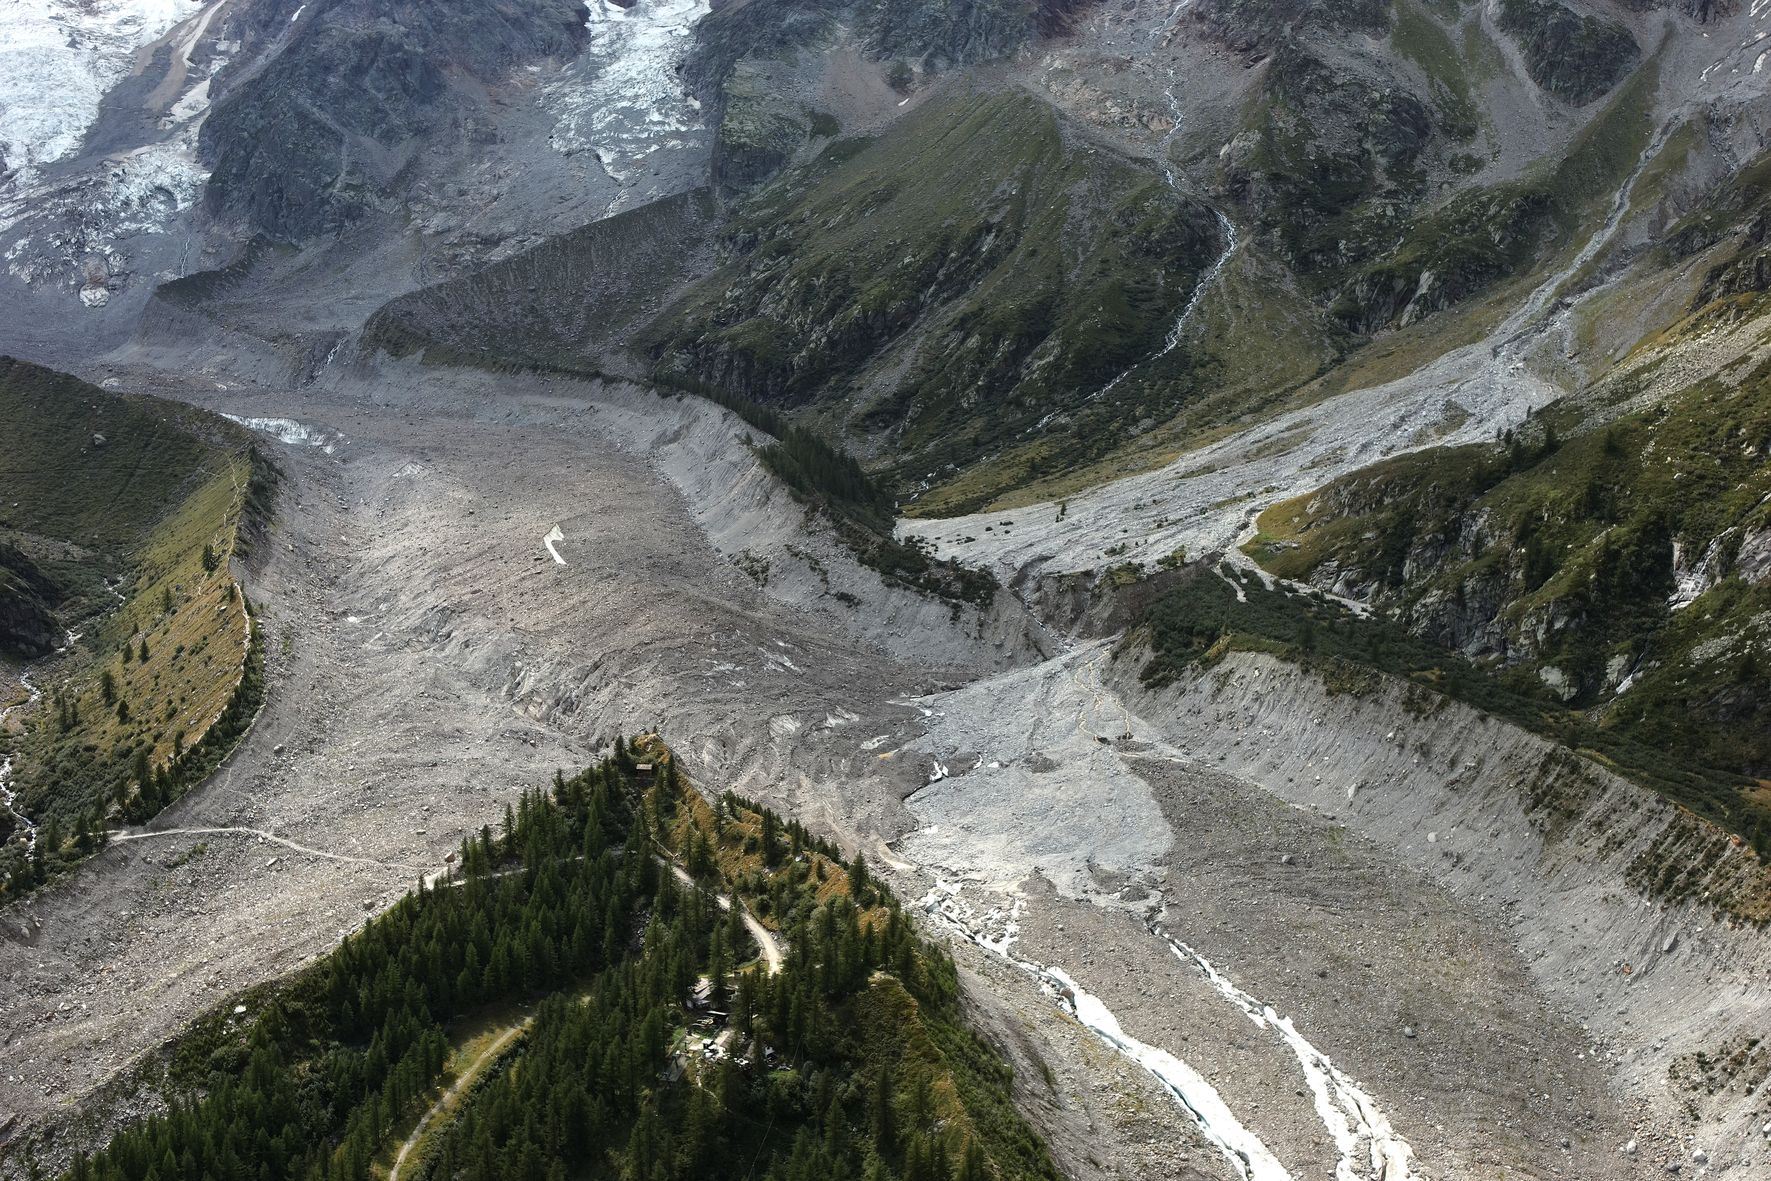
\includegraphics[height=4.8cm]{DJI_20230830144913_0181}
    }
    \subcaptionbox{\label{fig:1:belvedere_debris_flow:cam}}{
        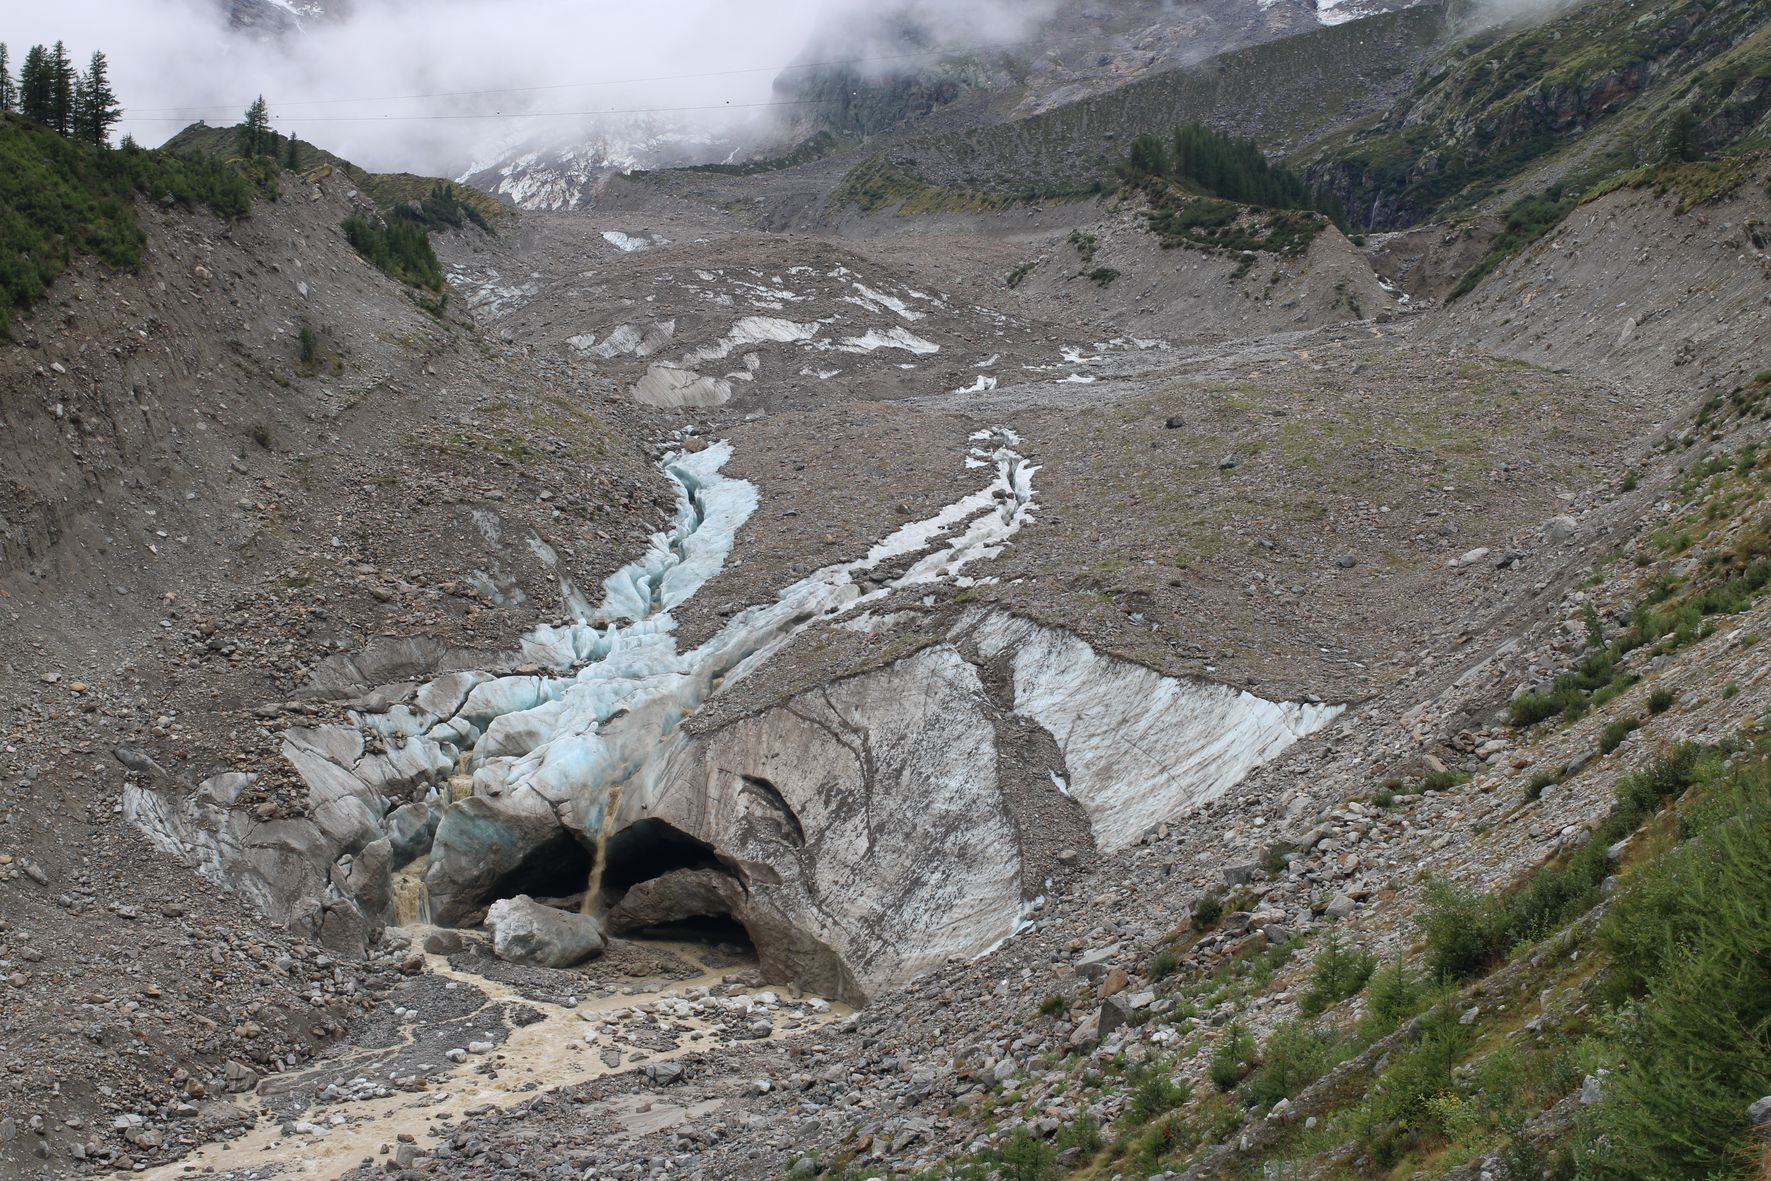
\includegraphics[height=4.8cm]{p1_20230828_155946_IMG_1457.jpg}
    }
    \caption{Impact of the August 27, 2023 debris flow on the Belvedere Glacier (Anscasca Valley, Italian Alps). \textbf{(a)} Aerial view acquired (August 30, 2023, author's photo) reveals the extent of debris accumulation within the Castelfranco gully and across the glacier's northern lobe; \textbf{(b)} Picture of the Belvedere Glacier northern lobe few hours after the debris flow event (August 28, 2023, 4:00 PM), captured by the fixed monitoring system. Note the 
    muddy channels carved into the glacier's surface. These channels are remnants of the powerful flow that washed away much of the debris.
    }
    \label{fig:1:belvedere_debris_flow}
\end{figure}

On August 27, 2023, a large debris flow occurred at the Belvedere Glacier (Anzasca Valley, Italian Alps)\footnote{\url{https://www.regione.piemonte.it/web/temi/protezione-civile-difesa-suolo-opere-pubbliche/protezione-civile/sorvolo-ghiacciai-monte-rosa-07092023}}.
The debris flow was triggered at the beginning of the steep Castelfranco gully, located at approximately \SI{3600}{\masl} on the streamwise-left side of the Belvedere Glacier northwest lobe (\figref{fig:1:belvedere_debris_flow}).
During the event, a volume of \SI{\sim 200000}{\cubic\meter} was accumulated on top of the Belvedere Glacier and obstructed the sinkhole that allowed the Castelfranco stream to flow below the ice sheet. 
This caused the water to stream on top of the glacier, carving deep grooves on the Belvedere Glacier (\figref{fig:1:belvedere_debris_flow:cam}). 
A large portion of the debris cumulated in the riverbed was transported towards the municipality of Macugnaga by the river Anza.
A previous event with similar characteristics but significantly smaller dimensions occurred in 2008 and was documented by \citet{Mortara2009}, who reported an estimation of a few thousand cubic meters of cumulated debris volume.

\begin{figure}[ht!]
    \centering
    \subcaptionbox{}{
        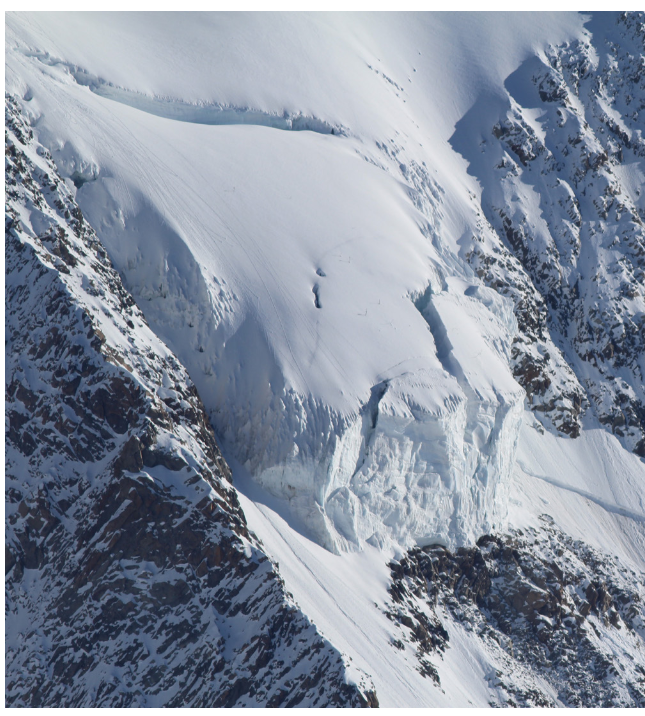
\includegraphics[height=5.3cm]{planpincieux_2}
    }
    \subcaptionbox{}{
        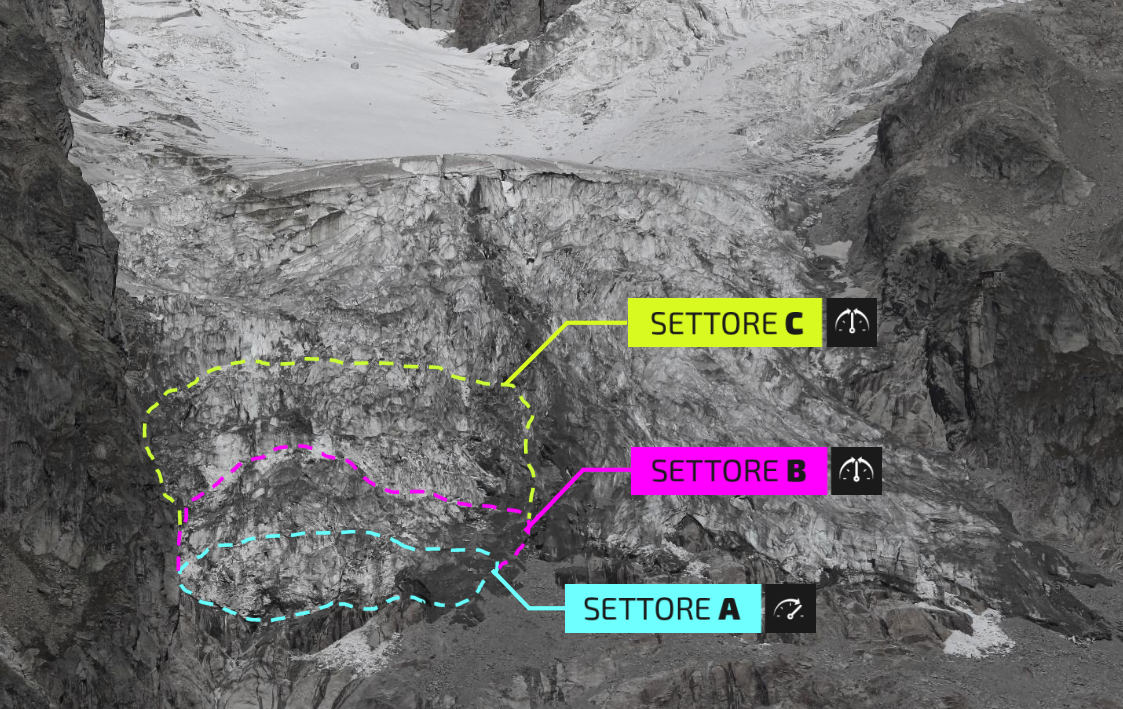
\includegraphics[height=5.3cm]{planpincieux_1}
    }
    \caption{Images of the Planpincieux Glacier (Mont Blanc Massif). (a) Close-up photo of the Whymper Serac. The fracture fractures in the frontal part of the serac, from where several ice break-offs are triggered, are clearly visible (photo Fondazione Montagna Sicura, 2020, \citet{chiarle2023}); (b) illustration of the Planpincieux Glacier with overlapped the area of three sectors identified by the permanent monitoring system based on their different kinematics properties (photo Fondazione Montagna Sicura, 2023, \citet{Giordan2020a}).
    }
    \label{fig:1:planpincieux}
\end{figure}

Another significant example of an ice failure-related hazard that demands continuous monitoring is the Planpincieux Glacier on the Italian side of the Grandes Jorasses in the Mont Blanc massif. 
The Planpincieux Glacier is a polythermal hanging glacier noted for its significant break-off activity (\figref{fig:1:planpincieux}).
The terminus of the Montitaz lobe features a 20-meter-high ice cliff, from which ice chunks exceeding \qty{50000}{\cubic\meter}  cubic meters frequently detach \cite{Giordan2020a}. 
The most recent major break-off occurred during the night of May 31 to June 1, 1998, when nearly the entire Whymper glacier, approximately \SI{\sim 150000}{\cubic\meter}, broke off, triggering an ice avalanche that reached the valley floor, fortunately without causing any damage \cite{Faillettaz2016, chiarle2023}. 
Additionally, this glacier was responsible for the deadliest ice failure event in the Italian Alps before the Marmolada tragedy: on August 2, 1993, an ice break-off exceeding \qty{80000}{\cubic\meter} killed eight mountaineers ascending the normal route of the Grandes Jorasses from the Boccalatte Hut \cite{Faillettaz2016, chiarle2023}.
For this reason, the glacier has been monitored since 2013 using a visual-based system installed at 2305 meters elevation and 3800 meters from the glacier\footnote{https://www.fondazionemontagnasicura.org/monitoraggio-planpincieux}. 
This system, developed by the Research Institute for Geo-Hydrological Protection (IRPI) of the Italian National Research Council (CNR) and the Safe Mountain Foundation (FMS), consists of two consumer-grade cameras powered by solar panels and remotely controlled, capturing one image per hour \cite{Dematteis2018, Giordan2020a}.
Additionally, a ground-based SAR (GBSAR) system captures images every 16 minutes, collecting over 2200 images during the study period, ensuring detailed monitoring of the glacier's movements \cite{Dematteis2018}.

In this context, systematically monitoring glaciers and related glaciological processes is crucial.
To thoroughly understand these complex systems, accurate observations are essential \citep{Kaab2005}.
A particular focus is usually placed on monitoring surface kinematics, as these can potentially offer early warning signs of impending instability or collapse events \citep{Faillettaz2015, Giordan2020a}.
Nevertheless, monitoring glaciers in remote areas and inaccessible terrains often presents logistical and safety challenges.
Therefore, remote sensing techniques are widely used because they allow scientists and technicians to observe glacial processes with minimal risk. 

\section{Remote and close-range sensing of alpine environments}

Remote sensing techniques have revolutionized our ability to study and monitor the dynamic landscapes of mountain environments. 
These techniques offer diverse ways to capture land surface characteristics from remote, providing insights into glacial processes and other natural phenomena in these often inaccessible regions.

Satellite-based remote sensing has been central in glacier monitoring for several decades \citep{Paul2007}. 
Satellites provide a wide-scale view of glacier evolution, from mapping glacier outlines from optical imagery or combinations of different bands \cite{Hall1995, Paul_2002, Winsvold2016} to deriving planimetric displacements using Digital Image Correlation (DIC) and estimating glacier surface velocities \cite{Scambos1992, Kaab2005, Scherler2008, altena_kaab_2020}, and estimating glaciers' mass balance \cite{Bamber2007, Berthier2016, Rabatel2017, Berthier2023}.
However, despite satellite remote sensing being essential for regional —or even global —glacier monitoring, the freely available satellite solutions lack the spatial and temporal resolution necessary to monitor small alpine glaciers and their rapid changes.
Additionally, satellite imagery primarily provides planimetric (2D) information, precluding the generation of 3D Digital Surface Models (DSMs) that would require multi-view acquisitions.

Synthetic Aperture Radar (SAR) offers advantages such as penetrating clouds and acquiring data regardless of illumination conditions \citep{Fang2016, Winsvold2018, Strozzi2020}. 
Techniques like InSAR can detect small movement along the satellite's line-of-sight (or even in 3D with multi-orbit acquisitions) in the presence of permanent scatter features \citep{schubert2013glacier}.
However, challenges arise with significant surface changes, as long satellite revisit times can lead to a loss of coherence between consecutive images, hindering accurate measurements of rapid glacier dynamics.
On the other hand, offset tracking on SAR amplitude images \citep{schellenberger2015sar}, while useful for mapping planimetric velocity, frequently suffers from the coarse resolution of free SAR satellite imagery.

Recent advances in Very High-Resolution Satellites (VHR) satellites such as World-View, Spot, Pleiades, and Pleiades Neo multi-view acquisitions enable meter or sub-meter resolution DSM generation from stereo pairs or triplets \citep{rupnik2018_VHR, Perko218, Tonolo2020}.
These satellites offer unprecedented spatial detail for glacier monitoring, yet limitations exist.
High commercial costs and the lack of a long historical image series compared to Landsat or Sentinel-2 restrict their applications to longer temporal scales.

Aerial or helicopter-based photogrammetry fills the critical gap between satellite-based and Unmanned Aerial Vehicles (UAVs)-based approaches, offering the potential for 3D reconstruction and DSM generation at the decimeter to sub-meter resolution in remote mountain areas \citep{poli2020use}. 
While the cost of photogrammetric flights remains a factor, the availability of regional mapping datasets presents a unique opportunity for long-term glacier monitoring.
In particular, historical aerial imagery allows for reconstructing glacier geometries far into the past \citep{Degaetani2021}, beyond the era of VHR satellites and offering valuable insights into the long-term evolution of alpine glaciers.

In the past decade, UAVs have emerged as powerful and cost-effective tools for small to mid-scale mapping.
In conjunction with advances in Structure-from-Motion (SfM) \citep{Westoby2012} and Multi-View Stereo (MVS) \citep{Seitz2006} algorithms,  UAVs enable the generation of high-resolution 3D point clouds, DSMs, and orthophotos for glacier studies. 
Their ease of deployment, minimal requirements, and ability to access remote areas safely make them invaluable in glacial environments \citep{immerzeel2014, Chudley2019, ioli2021mid}. 

Several examples of UAV and photogrammetry applications for cryosphere monitoring can be found in the literature~\citep{Bhardwaj2016, Gaffey2020}.
These studies cover diverse environments and methodological approaches.
For instance, \citet{Whitehead2013} employed fixed-wing UAVs and piloted helicopters with low-cost cameras to generate orthophotos and DSMs of the Fountain Glacier in the Canadian Arctic, demonstrating the applicability of UAVs for glacier mapping even in challenging conditions. 
Similarly, \citet{immerzeel2014} and \citet{kraaijenbrink2016} used fixed-wing UAVs to evaluate seasonal surface velocities of the debris-covered Lirung Glacier in Nepal, highlighting the potential for analyzing glacier dynamics at fine temporal scales.
\citet{Gindraux2017} further investigated the impact of Ground Control Point (GCP) quantity and distribution on the accuracy of UAV-derived glacier DSMs, and she proposed a technique based on the joint usage of DIC on both DSMs and orthophotos to derive glacier kinematics.
The growing body of recent work \citep{Benoit2019, Chudley2019, Jouvet2020, Cao2021,  ioli2021mid, Lamsters2022, belloni2023} showcases the widespread adoption of UAVs and low-cost photogrammetry in glacier monitoring. 
These studies demonstrate their effectiveness in capturing high spatial resolution data while minimizing the need for extensive and potentially hazardous in-situ operations.
This underscores the potential of UAVs to track glacier evolution at unprecedented levels of detail over extended periods \citep{ioli2021mid, belloni2023}.

Nevertheless, continuous in-situ monitoring with sub-seasonal temporal frequency using UAVs can be logistically challenging.
While UAV photogrammetry excels in spatial resolution, reconstruction accuracy, and flexibility, capturing short-term glacier dynamics at a high temporal frequency (e.g., daily) still necessitates permanent in-situ monitoring systems. 
Short-term observations are crucial for deeply understanding these rapidly evolving glaciers and their associated processes.
Low-cost time-lapse camera systems can provide daily observations for studying sub-seasonal glacier kinematics and responses to external factors within a warming climate \cite{Messerli2015}.  
Due to their revisit time limitations, neither satellite-based nor aerial/UAV photogrammetric techniques can provide this level of continuous data.

Recently, terrestrial SAR \cite{Luzi2007} and permanent Terrestrial Laser Scanners (TLS) \cite{Hendrickx2022, Voordendag2023} have gained attention for short-term monitoring. 
SAR's all-weather, day-and-night capabilitises are ideal for real-time monitoring and early warning systems \citep{Noferini2009, Dematteis2017_sar}. 
However, the high costs, complex logistics, and often site-specific focus of ground-based SAR and permanent TLS limit their widespread application for regional-scale monitoring.
Fixed time-lapse cameras present a cost-effective alternative for gathering qualitative and quantitative data on glacier dynamics~\citep{Maas2006, Messerli2015, Giordan2016, James2016}.

Monitoring glacier surface kinematics is especially important, as it can provide early indications of impending instability \citep{Faillettaz2015}.
A powerful approach for deriving glacier flow velocity using close-range or remote sensing involves DIC or feature tracking algorithms \cite{ahn_box_2010, Giordan2016, Hadhri2019}.
At its core, DIC works by tracking distinctive pixel patterns across a time series of images.
It begins by dividing the reference image into small subsets, known as templates or interrogation windows. 
For each template, DIC uses cross-correlation techniques to identify the most similar region within a designated search area in the subsequent image.
This can be done in the spatial domain \citep{Scambos1992} or frequency domain \citep{rolstad1997}.
The displacement between the template’s original position and this matching region represents the movement of the tracked feature on the glacier's surface.
DIC is now widely used for analyzing glacier movement using various remote sensing data sources, including optical satellite imagery \citep{Scambos1992, Scherler2008, Heid2012_evaluation_xcorr}, high-resolution orthophotos derived from aerial or UAV photogrammetry \citep{immerzeel2014, Chudley2019, ioli2021mid}, as well as terrestrial time-lapse cameras \cite{Messerli2015, Giordan2016}. 

While monoscopic time-lapse cameras effectively derive surface kinematics using DIC, a richer 3D reconstruction requires a multi-camera setup. 
However, the constraints of mountainous terrain can force camera placement into less-than-ideal positions. 
This often results in challenging acquisition geometries, such as very long baselines or strongly convergent angles \citep{ioli2024deep}.
Traditional image matching techniques, that rely on handcrafted feature descriptors (e.g., SIFT, Kaze, ORB), struggle with the substantial variations introduced by these geometries.  Perspective shifts, occlusions, and the difficulty of reliably matching features across dramatically different views hinder accurate 3D reconstruction. 
These limitations require innovative approaches to ensure robust feature matching and scene reconstruction in these complex environments.
DL-based matching techniques surpass traditional methods' adaptability to wide baselines, significant radiometric differences, and complex geometric distortions \cite{Yao_2021}. 
Research in this domain has progressed rapidly, with models specifically designed to handle oblique images, historical image sets, and low-quality consumer cameras.

\section{The Belvedere Glacier}\label{sec:1:belvedereglacier}

The Belvedere Glacier (Randolph Glacier Inventory code RGI60--11.02858) is an alpine
glacier in the Anzasca Valley (Italy), on the east side of the Monte Rosa Massif (N
\ang{45;58} E \ang{7;55}) (\figref{fig:1:studyarea}).
The lower part of the Belvedere Glacier is a temperate debris-covered glacier that
covers an area of \SI{\sim1.8}{\kilo\meter\squared} and extends from an altitude of \SI{\sim2250}{\masl} to \SI{\sim1800}{\masl}.
This region is characterized by a gentle slope, and it is fed by icefalls and snow
avalanches coming from the Monte Rosa East Face \citep{Haeberli2002}. 
The Belvedere Glacier splits into two lobes in its low-relief sector, reaching \SI{\sim1800}{\masl}.
The northern lobe, in particular, ends with a prominent ice cliff, from which the River
Anza springs.

Similarly to Miage Glacier (Monte Bianco, Valle d’Aosta), the Belvedere Glacier is almost entirely covered by rocks and boulders with dimensions ranging from a few decimetres to
some meters, which makes it a \textit{black glaciers}.
Due to the global warming trend, the number of black glaciers along the Italian Alps is
rising \citep{Diolaiuti2003}.
\marginpar[Note 1]{
    
\includegraphics[width=\marginparwidth]{qr_thebelvedereglacier.png}
    % \footnote{\url{www.thebelvedereglacier.it}}
}
Up to the beginning of the century, the~debris cover helped to compensate the effect of
the increased temperature, establishing a negative feedback in the temperature-ablation
relationship~\citep{Roethlisberger1985,Diolaiuti2003}.
However, in recent years, the debris cover protection has not been sufficient to limit
the glacier~retreat.

\begin{figure}
    \centering
    \subcaptionbox{\label{fig:1:studyarea:map}}{
        \includegraphics[height=5cm]{belvedere_location.png}
    }
    \subcaptionbox{\label{fig:1:studyarea:pic}}{
        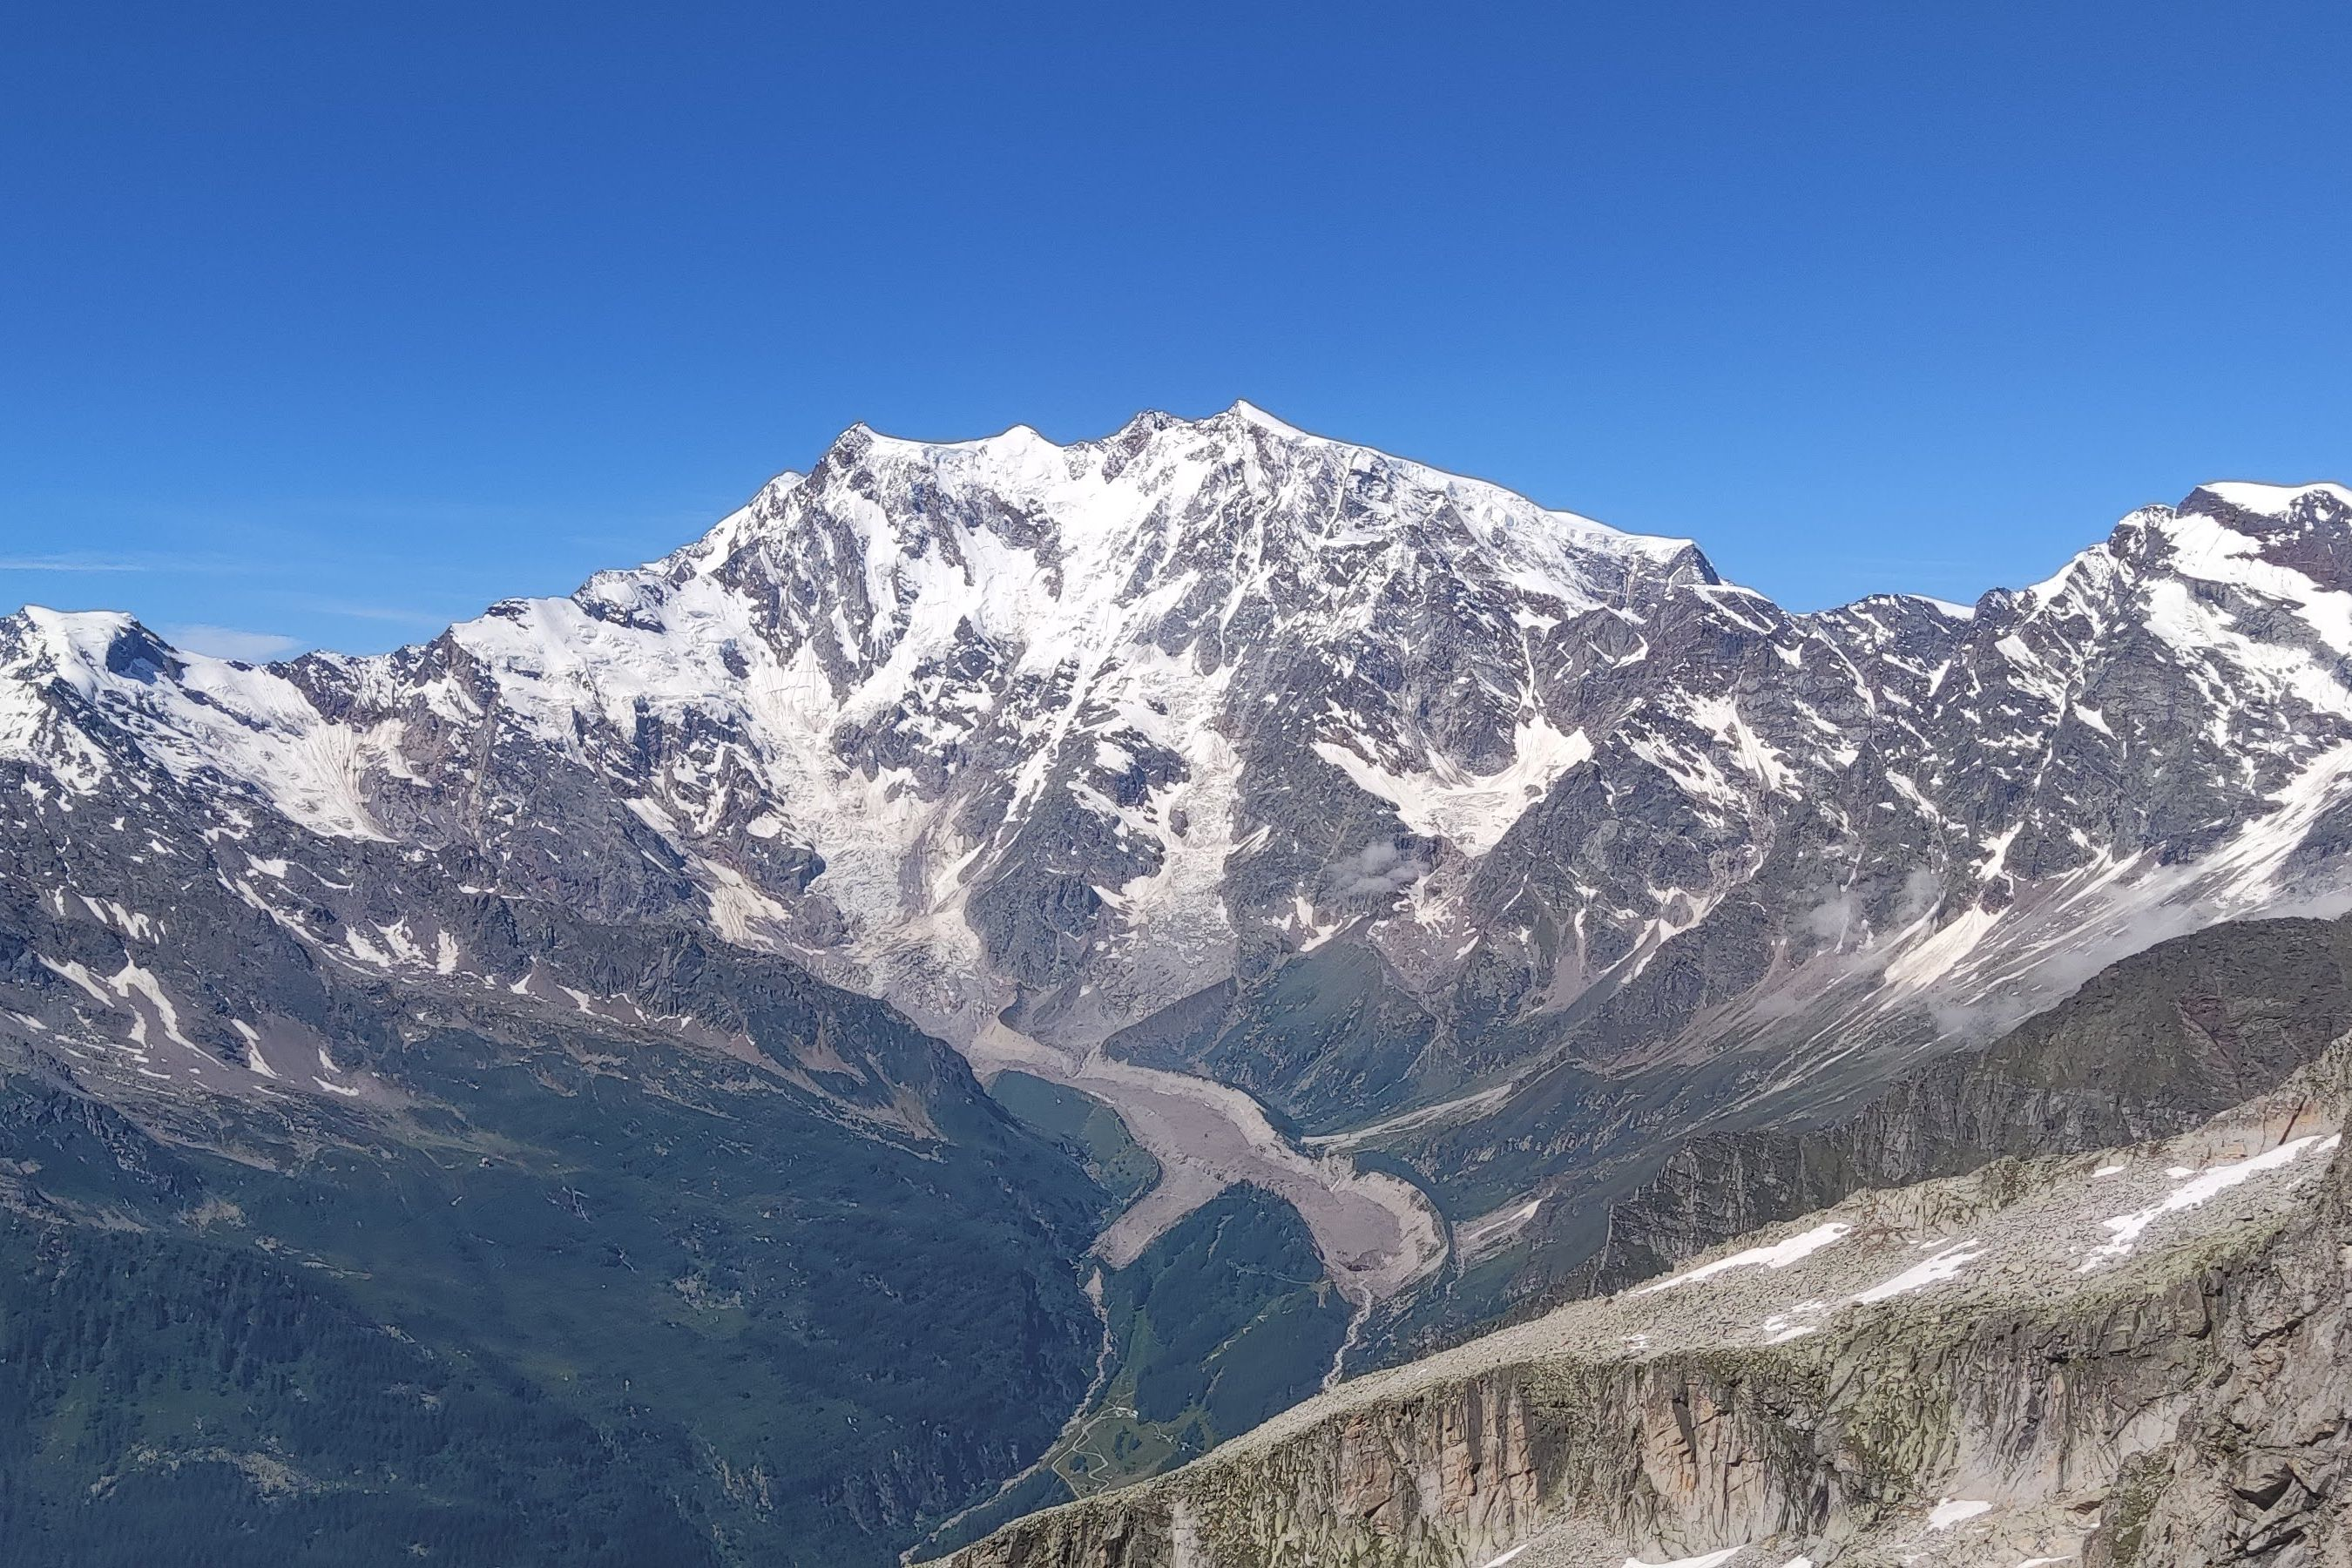
\includegraphics[height=5cm]{belvedere_pic.jpg}
    }
    \caption{(a) Location of Belvedere Glacier, base map (source: Swisstopo
        www.geo.admin.ch); (b) Picture of the Belvedere Glacier taken from the nearby Monte Moro.}
    \label{fig:1:studyarea}
\end{figure}

In the past, several hazardous events originated from the Belvedere Glacier, such as floods
and slope instability, threatened the nearby village of Macugnaga and the Zamboni Zappa
Hut, at 2070 m a.s.l. \citep{Kaab2004}.
At the beginning of the 21st century, the Belvedere Glacier was characterized by a
particular surge-type dynamics  \citep{Haeberli2002}.
During the late 1990s, the~surface speeds of the whole glacier were ranging between
\SIlist{30;45}{\meter\per\year}~\citep{Roethlisberger1985, Kaab2005}.
During 2000--2001, an accelerated flow in the Monte-Rosa Glacier produced a wave of
compression-decompression stresses and strains in the Belvedere Glacier.
Surface velocities soared: values up to \SI{200}{\meter\per\year} were observed
photogrammetrically during autumn 2001~\citep{Kaab2004}.
The ice thickness increased more than~\SI{20}{\meter} and the wave travelled downwards,
creating a depression area in the accumulation zone that was filled by a super-glacial
lake, the Lago Effimero~\citep{Haeberli2002, Mortara2009}.

During spring 2002, the large depression at the foot of the Monte Rosa east face, caused by the surge-type movement, was temporarily filled by a lake with a volume of \SI{3e6}{\cubic\meter}, the so-called \textit{Lago Effimero} (\textit{short-lived lake}).
Recognizing the potential danger of an outburst flood, the Italian Civil Defense Department rapidly 
implemented emergency measures, including evacuating parts of Macugnaga village, installing automatic 
alarm systems and pumps, and initiating detailed scientific investigations. 
Reduced meltwater input in July 2002, combined with natural subglacial drainage, stabilized and subsequently 
lowered the lake level.
However, the lake reformed in the spring of 2003, bursting out in mid-June without causing significant damage \citep{Kaab2004}.

% \textcolor{red}{Expand this part and add more pics with old and recent events}

% The northern lobe of the Belvedere Glacier is concurrently experiencing a fast retreat:
% in the past few years, an average retreat of \SI{\sim20}{\meter\per\year} was documented
% \citep{Ioli2022} and it is actively changing every day due to ice falls and collapses.


\section{Objectives}

This thesis explores the potential of multi-scale and multi-temporal photogrammetry 
for monitoring alpine glaciers, focusing on the debris-covered Belvedere Glacier in the Italian Alps.

This investigation integrates a spectrum of photogrammetric techniques.  
Firstly, historical aerial imagery analysis provides a long-term perspective on decades-long geomorphological changes at the meter scale.  
Secondly, in-situ UAV acquisitions enable annual reconstructions of glacier morphology, allowing for precise change analysis at a high spatial resolution.  
Finally, permanent in-situ monitoring using a low-cost stereo camera system allows for capturing the short-term dynamics of this rapidly changing environment.

% \textcolor{red}{Add figure of multi-temporal/multi-scale}

This study uses archival aerial photogrammetry data collected by public agencies during mapping flights to investigate the glacier's long-term evolution.
This technique allowed the reconstruction of past glacier morphology from 1977 to 2009, with approximately decadal intervals between models.  
The historical knowledge gained through this method is invaluable in documenting a natural heritage rapidly disappearing due to climate change. 
Of particular interest, archival photogrammetry reveals a significant period of glacier expansion in the early 21st century, allowing precise quantification of the increase in ice volume and glacier thickness.

This work integrates low-cost UAVs and GNSS for close-range photogrammetric monitoring to understand the glacier's current evolution.
Annual in-situ surveys since 2015 provide a periodic and highly accurate record of the evolution. 
Through these UAV surveys, centimeter-scale resolution enables detailed mapping of the dynamic environment, including precise quantification of glacier volume loss and study of variations in glacier flow rate.

However, alpine glacier dynamics are inherently non-linear, with a pronounced acceleration of processes in summer compared to winter.  
This trend has intensified in recent years due to the increasing frequency of hot and dry summers associated with climate change. 
While annual high-precision in-situ measurements provide essential insights into long-term geomorphological evolution, they lack the temporal resolution to fully capture the short-term kinematics of the glacier, which are crucial for
understanding the relationship between glacier dynamics and external drivers such as air temperature.
To address this need, a permanent monitoring system based on low-cost stereo cameras has been designed and installed on Belvedere Glacier. 
This system allows daily observations of glacier motion at a local spatial scale,
providing the high-frequency data needed for in-depth kinematic analysis.

This thesis describes the technical design and implementation of a low-cost glacier monitoring system and the development of novel software tools for extracting relevant information from stereo camera images via photogrammetric processing. 
A new pipeline was designed and published to overcome the limitations of existing software in handling images with extremely wide baselines. 
This pipeline allows the analysis of time-series point clouds and the extraction of metrics such as velocity, volume variations, and displacement.

The harsh mountain environment was a significant challenge, which constrained the camera placement.
This resulted in extremely wide baselines and significant viewpoint differences.  
These conditions made it difficult to find corresponding points using traditional local feature-matching techniques and hindered 3D reconstruction using existing commercial and open-source photogrammetric software.
To overcome this obstacle, a novel pipeline was developed using state-of-the-art deep-learning algorithms for robust feature matching that successfully overcomes the limitations of wide baseline stereo image processing.

This thesis presents a successful pilot test of the low-cost glacier monitoring system.
The current uses only two cameras installed at the northwest terminal lobe of the Belvedere glacier, focused on the terminal ice cliff, the portion of the glacier experiencing the most severe retreat and fast evolution. 
However, the system needs to be scaled up to achieve a more comprehensive and robust monitoring framework capable of capturing the glacier's entire dynamics. 
Expanding the camera network will increase the coverage and significantly improve the quality of daily 3D reconstructions through greater data redundancy.
Motivated by this potential, the final part of this thesis focuses on developing a flexible multi-view library. 
This library enables image matching using state-of-the-art deep learning algorithms and traditional handcrafted features. 
Crucially, it integrates seamlessly with existing photogrammetric software for streamlined 3D reconstruction, thus supporting the monitoring system's future expansion.


\section{Thesis outline}

This thesis is introduced in \textbf{\chref{ch:1}}. 
This chapter presents the motivation, the research problem, and the objectives of the thesis.
It introduces the Belvedere Glacier as a primary case study. It presents an overview of remote and close-range sensing techniques for alpine environments, focusing on image-based techniques for glacier monitoring at different spatial and temporal scales.

\textbf{\chref{ch:2}} analyzes the historical evolution of Belvedere Glacier (1977-2009) using archival aerial photogrammetry with sub-meter spatial resolution and decadal survey intervals.

\textbf{\chref{ch:3}} describes the annual UAV and GNSS survey methodology for contemporary monitoring of Belvedere Glacier (2015-2023).  
SfM-MVS techniques generate annual 3D models, orthophotos, and DSMs with decimeter resolution.
Glaciological analysis reveals complex spatial and temporal patterns in surface velocities, volume variations, and thinning effects.

\textbf{\chref{ch:4}} presents a novel low-cost stereo camera system for daily monitoring of a section of Belvedere Glacier (May-November 2022).
Deep learning algorithms overcome the challenges of large baselines, enabling accurate 3D reconstruction, surface velocity estimation, and quantification of ice loss with daily frequency. 

\textbf{\chref{ch:4}} describes Deep-Image-Matching (DIM), a novel open-source toolkit for wide-baseline, multi-view image matching in complex scenarios. 
DIM's robustness, flexibility, and integration capabilities make it a powerful tool for expanding the use of deep learning in photogrammetry. 

\textbf{\chref{ch:conclusion}} synthesizes the key findings of the thesis, highlighting their significance within glaciological research and the broader context of climate change.  
It emphasizes the unique long-term insights gained for Belvedere Glacier and the transformative tools developed for broader glacier monitoring. 
The commitment to open science and data sharing encourages collaboration and future research.

% References
\makechapterbibliography{}
\graphicspath{{figures/chapter2/}}

\chapter{Back to the past: reconstructing glacier geometry with historical aerial images
  (1977-2009)}\label{ch:2}

\vfill

\newthought{This chapter is based on:}

\noindent De Gaetani, C. I., Ioli, F., \& Pinto, L. (2021). Aerial and UAV Images for
Photogrammetric Analysis of Belvedere Glacier Evolution in the Period 1977–2019. Remote
Sensing, 13(18), 3787. \url{https://doi.org/10.3390/rs13183787}

\newpage

\section{Introduction}\label{sec:2:introduction}

\section{Datasets}\label{sec:2:datasets}

\subsection{Historical Aerial Datasets of 1977, 1991 and 2001}

\subsection{Digital Aerial and UAV Datasets of 2009 and 2019}

\subsection{GNSS Survey for Block Georeferencing}

\section{Methods}\label{sec:2:methods}

\section{Discussion}\label{sec:2:discussion}

% References
% \bibliography{references}
% \addcontentsline{toc}{section}{References}
% \bibliographystyle{apacite}

\graphicspath{{figures/chapter3/}}
\onehalfspacing

\chapter{UAV photogrammetry for annual glacier reconstruction (2015-2023)}\label{ch:3}

\vfill

\newthought{This chapter is based on:}

\begin{itemize}
    \item \noindent Ioli, F., Bianchi, A., Cina, A., De Michele, C., Maschio, P., Passoni, D., \& Pinto, L. (2022). Mid-Term Monitoring of Glacier's Variations with UAVs: The Example of the Belvedere Glacier. Remote Sensing, 14(1), 28. \url{https://doi.org/10.3390/rs14010028}
    \item Ioli, F., De Gaetani, C., Barbieri, F., Gaspari, F., Pinto, L., \& Rossi, L. (2024). Belvedere Glacier long-term monitoring Open Data [Data set]. Zenodo. \url{https://zenodo.org/doi/10.5281/zenodo.7842347}
\end{itemize}

\newpage

\section{Introduction}\label{sec:3:intro}

This chapter investigates the potential of high-resolution UAV photogrammetry and in-situ GNSS measurements to comprehensively monitor the Belvedere Glacier. 
Originally, our understanding of glacier dynamics was constrained by the limitations of traditional aerial photogrammetry, which provided data at approximately decadal intervals and sub-meter resolution. 
A UAV-based approach offers a paradigm shift, enabling annual reconstructions with sub-decimeter resolution.
With this enhanced capability, we can delve into the glacier's yearly kinematics, gaining deeper insights into its evolution and responses to climate change.

The Belvedere Glacier monitoring campaign, which started in 2015, was designed and conducted jointly by the Department of Civil and Environmental Engineering (DICA) of Politecnico di Milano and the Department of Environment, Land and Infrastructure Engineering (DIATI) of Politecnico di Torino. 
Moreover, the DREAM projects (DRone tEchnnology for wAter resources and hydrologic hazard Monitoring), involving teachers and students from Alta Scuola Politecnica (ASP) of Politecnico di Torino and Milano, contributed to the campaign from 2015 to 2017.

Every year, fixed-wing UAVs and quadcopters were used to remotely sense the glacier and build high-resolution 3D photogrammetric models, DSMs, and orthophotos.
The series of point clouds was used to estimate the glacier volume variations and estimate the thinning of the glacier.
The orthophotos and the DSMs were also used to investigate the glacier kinematics and derive ice flow velocity and glacier retreat. 
This was carried out by exploiting DIC techniques to track the movement of the glacier surface.

The Belvedere Glacier monitoring campaign has produced a rich dataset of GNSS measurements, 3D point clouds, DSMs, and orthophotos. 
Recognizing the transformative potential of open science, we have made this entire dataset publicly available, and we have also developed a suite of web-based tools to make the data user-friendly for researchers and non-experts\footnote{\url{https://thebelvedereglacier.it/}}.
This chapter will finally describe the solutions to promote the widespread use of our monitoring data, accelerate scientific progress in glacier research, and encourage knowledge sharing across the scientific community.

\section{Instruments and datasets}\label{sec:3:instrument}
 
This section introduces the data acquired in this study from 2015 to 2023, including the periodic GNSS measurements of targets deployed over the glacier and UAV images acquired to build the photogrammetric reconstructions.

\subsection{GNSS measurements}\label{sec:3:gnss}

Yearly GNSS measurements of permanent targets deployed across the glacier were conducted. 
These targets served a dual purpose: as GCPs/CPs for photogrammetric block processing and as high-accuracy 
reference points for evaluating glacier kinematics derived from photogrammetry. 
The targets were materialized using square cross patterns printed on polypropylene sheets and anchored to 
large rocks and boulders (\figref{fig:3:belvedereGCP}b).

Approximately 25 targets were deployed on the glacier itself (designated as \textit{moving targets} or 
\textit{M\#} in \figref{fig:3:belvedereGCP}a), while 24 targets were placed on stable areas along the moraines 
(labelled as \textit{stable targets} or \textit{S\#} in \figref{fig:3:belvedereGCP}a). 
Annually, we evaluated the condition of each target. 
Damaged or destroyed targets were replaced with new polypropylene plates, maintaining the original center location using the existing plugs. 
Over time, some targets were lost and replaced with new ones near the original locations (e.g., M29bis).

All targets were surveyed with dual frequency geodetic quality GNSS receivers: 
Leica Viva GS14 and Leica GPS1200+.
The measurements were framed within the official Italian reference system ETRF2000
at the epoch 2008.0, projected in UTM 32N (RDN2008 / UTM zone 32N, EPSG:7791).
The measurement techniques employed in the survey have evolved.
Before 2021, target positions on the lower glacier, where GSM network coverage was available, were determined using nRTK relative to CORS permanent stations (HxGN SmartNet or SPIN GNSS). 
These points were occupied for at least 20 seconds. 
In contrast, upper glacier targets were surveyed using static sessions of approximately 10 
minutes, with raw data post-processed relative to local master stations located in stable areas (S12 or S20, see \figref{fig:3:belvedereGCP}a).
Since 2021, GNSS measurements have been conducted in RTK mode using a local base station (\textit{S12} or \textit{S20}).
A radio link connection streamed the real-time corrections from the base to the rover. 
This approach has significantly reduced measurement time in the upper glacier, requiring seconds rather than minutes per occupation, as was for static processing of the upper glacier targets.
Additionally, the local-base RTK method improves internal coherence among measurements, 
as well as tropospheric and ionospheric error modeling due to shorter baselines compared to 
the nRTK approach.

The accuracy of GNSS measurements was evaluated empirically by comparing repeated
measurements over stable targets carried out in different years.
RMSE of \qty{1.5}{\centi\meter} in planimetry and \qty{3}{\centi\meter} in elevation were
obtained.

\begin{figure}
    \centering
    \subcaptionbox{\label{fig:3:studyarea:map}}{
        \includegraphics[width=.6\textwidth]{belvedereGCP.png}
    }
    \subcaptionbox{\label{fig:3:studyarea:pic}}{
        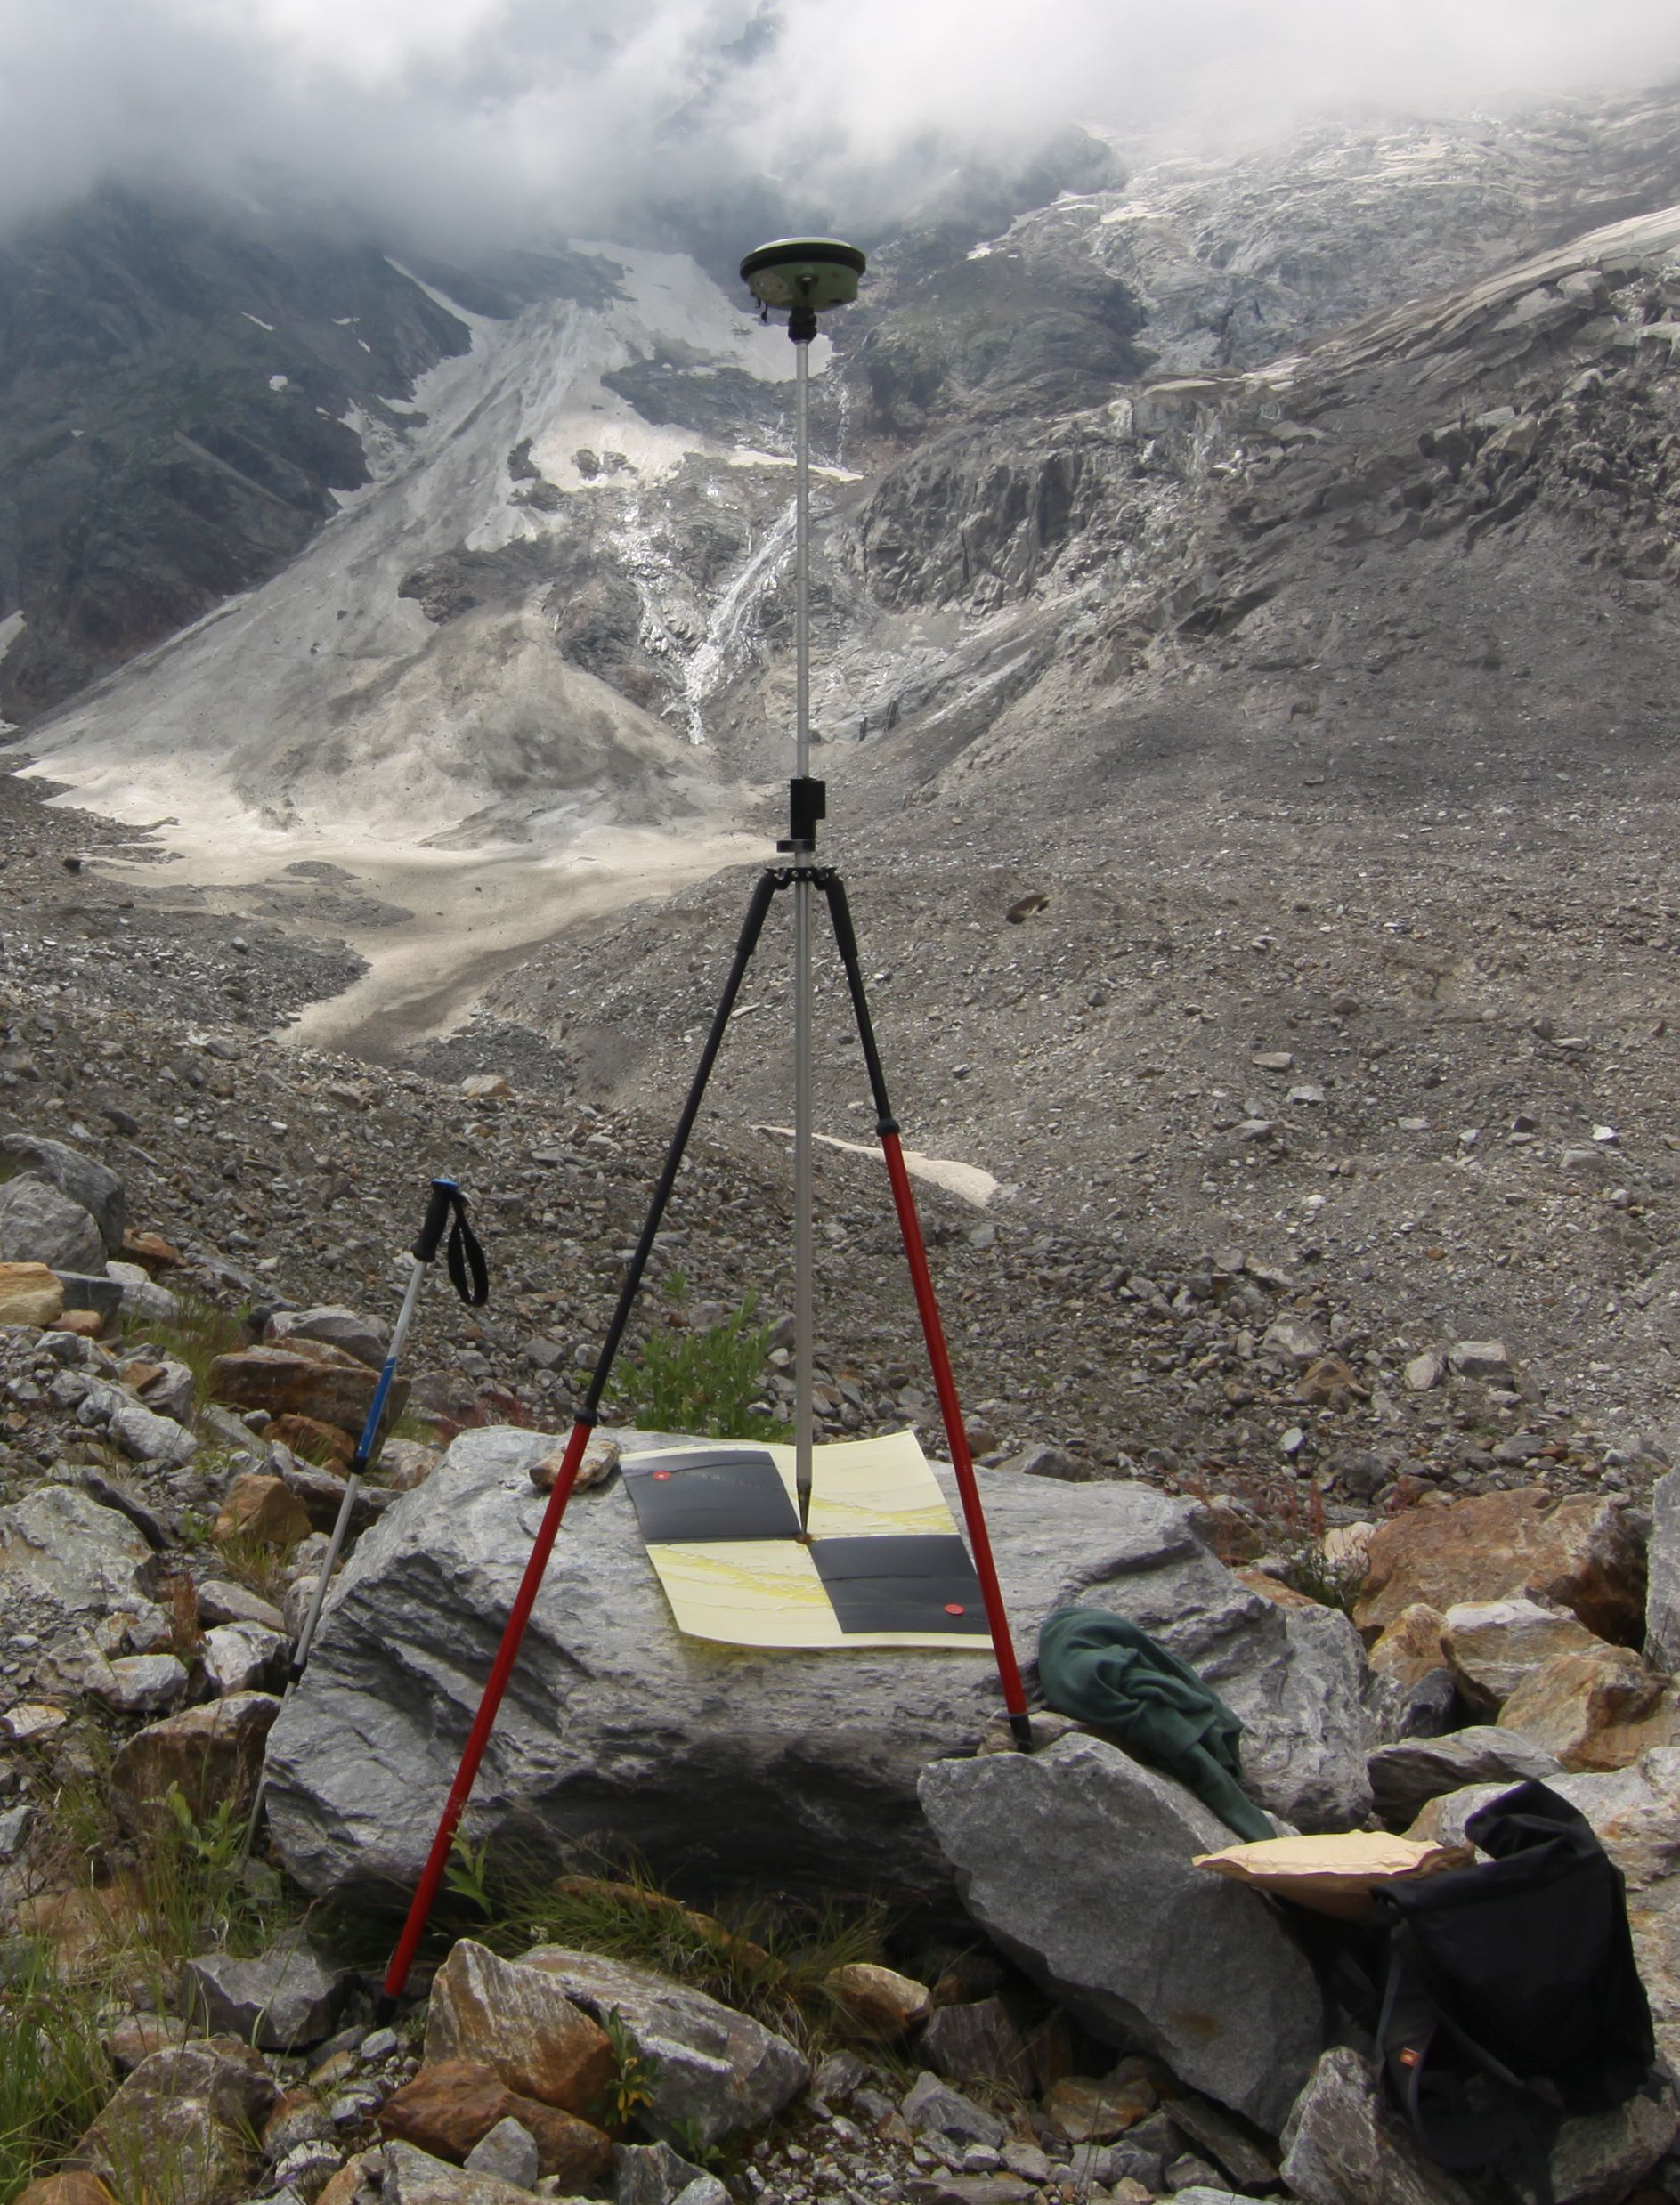
\includegraphics[width=.35\textwidth]{target.jpg}
    }
    \caption{(\textbf{a}) Location of the targets used for the
        photogrammetric surveys. For~each year, a~subset of the targets were used as GCPs, while the remaining as~CPs; (\textbf{b}) an example of a photogrammetric target deployed over the glacier moraine.}
    \label{fig:3:belvedereGCP}
\end{figure}


\begin{table}[p]
    \small
    \centering
    \caption{Summary of the characteristics of the surveys.}
    \begin{tabular}{c  m{1.8cm} m{3.5cm} m{4.2cm} c c c }
        \toprule
        Year                                                              & Date
                                                                          & UAV
                                                                          & Camera
                                                                          & GSD
                                                                          & GCP
                                                                          & CP
        \\
                                                                          &
                                                                          &
                                                                          &
                                                                          & [m/px]
                                                                          & [\#]
                                                                          & [\#]
        \\
        \midrule
        2015                                                              & A.
        8.10\newline B. 23.10                                             &
        SenseFly eBee                                                     & Canon
        PowerShot S110                                                    & 0.07
                                                                          & 24
                                                                          & 11
        \\[4mm]
        2016                                                              & 20.10
                                                                          & SenseFly eBee
                                                                          & Canon
        PowerShot S110                                                    & 0.09
                                                                          & 31
                                                                          &
        15
        \\[4mm]
        2017                                                              & A.
        5.10\newline B. 15.11\newline C. 16.11                            & A. SenseFly
        eBee \newline B. SenseFly eBee Plus\newline  C. DJI Phantom 4 Pro & A. Canon
        PowerShot
        S110  \newline B. SenseFly S.O.D.A \newline C. DJI FC6310         & 0.06
                                                                          & 27
                                                                          & 8
        \\[4mm]
        2018                                                              & 23-25.07
                                                                          & Parrot Disco
                                                                          & Hawkeye
        Firefly 8S                                                        & 0.05
                                                                          & 27
                                                                          &
        13
        \\[4mm]
        2019                                                              & 29.07-2.08
                                                                          & Parrot Disco
                                                                          & Hawkeye
        Firefly 8S                                                        & 0.06
                                                                          & 26
                                                                          &
        10
        \\[4mm]
        2020                                                              & A. 26-27.07
        \newline B. 9.08                                                  & A.
        Parrot Disco\newline B. DJI Phantom 4 Pro                         & A. Hawkeye
        Firefly 8S\newline B. DJI FC6310                                  &
        0.05                                                              & 29
                                                                          & 12
        \\[4mm]
        2021                                                              & 29.07-2.08
                                                                          & DJI Matrice 210 V2
                                                                          & DJI ZenMuse x5s
                                                                          & 0.04
                                                                          & 23
                                                                          &
        9
        \\[4mm]        
        2022                                                              & 28.07-29.07
                                                                          & DJI Matrice 300 RTK
                                                                          & DJI Zenmuse P1 - 35 mm
                                                                          & 0.03
                                                                          & 22
                                                                          &
        19
        \\[4mm]
        2023                                                              & 25.07-27.07
                                                                          & DJI Matrice 300 RTK
                                                                          & DJI Zenmuse P1 - 35 mm
                                                                          & 0.03
                                                                          & 23
                                                                          &
        9
        \\[4mm]        
        \bottomrule

    \end{tabular}
    \label{tab:3:datasets}
\end{table}

\begin{table}[p]
    \centering
    \small
    \caption{Summary of the characteristics of the cameras employed.}
    \begin{tabular}{c c c c c c}
        \toprule
        Camera                        & Sensor                        & Sensor Size
                                      & Focal length                  & Image size
                                      & Pixel size
        \\
                                      &                               &
        [\SI{}{\milli\meter\squared}] & \newline[\SI{}{\milli\meter}] & [\SI{}{\pixel}]
                                      & \newline[\SI{}{\micro\meter}]
        \\

        \midrule
        Canon PowerShot S110          & 1/1.7" \acs{cmos}                   & $7.44\times5.58$
                                      & 5.2                           & $ 4000 \times
            3000
        $                             & 1.9
        \\
        SenseFly S.O.D.A              & 1" CCD                        & $13.2\times8.8$
                                      & 10.6                          & $5472 \times
        3648$                         & 2.4
        \\
        DJI FC6310                    & 1" CMOS                       & $13.2\times8.8$
                                      & 8.8                           & $5472 \times3648$
                                      & 2.4
        \\
        Hawkeye Firefly 8S            & 1/2.3" CMOS                   & $6.17\times4.56$
                                      & 3.8                           & $5472 \times3648$
                                      &
        1.34
        \\
        DJI ZenMuse x5s               & 4/3" CMOS                     & $17.3\times13$
                                      & 15                            & $5280 \times
        3956$                         & 3.3 
        \\
        DJI Zenmuse P1 - 35 mm        & FullFrame CMOS                & $35.9\times24$
                                      & 35                            & $8192 \times
        5460$                         & 4.4
        \\
        \bottomrule
    \end{tabular}
    \label{tab:3:camere}
\end{table}


\subsection{UAV flights}\label{sec:3:uav-flights}

The long duration of the monitoring campaign, the challenging environment, and the involvement of multiple research groups led to the use of various UAV platforms and cameras over time. 
\tabref{tab:3:datasets} provides a detailed summary of the equipment (UAV and camera) employed while \tabref{tab:3:camere} lists the sensor and lens specifications for each camera.

In 2015 and 2016, a ready-to-fly fixed-wing SenseFly eBee equipped with a compact camera, Canon PowerShot S110, was used for whole glacier surveys.
Due to technical problems, the year 2017 saw the use of different UAVs (both fixed-wing and quadcopters) and camera combinations (\tabref{tab:3:datasets}). 
From 2018 to 2020, a low-cost recreational Parrot Disco FPV fixed-wing UAV (wingspan 1.15 m, weight 750 g) was adapted to carry a lightweight Hawkeye Firefly 8S action camera.

In 2021, a professional-grade DJI Matrice 210 V2 quadcopter was employed, carrying a 
DJI ZenMuse X5s camera featuring a Micro 4/3 sensor and a 15 mm lens. 
Since 2022, the UAV platform has been upgraded to a DJI Matrice 300 RTK quadcopter
with a full-frame DJI Zenmuse P1 camera and a DL 35 mm F2.8 LS ASPH lens.
While this setup offered superior image quality, the longer focal length required 
higher flight altitudes to maintain a consistent GSD with the previous surveys.
Furthermore, the DJI Matrice 300 RTK was equipped with an RTK GNSS receiver, enabling 
decimeter-level accuracy in recording the camera position for each shot. 
This precision was achieved through a local GNSS base station positioned near the take-off 
location, which streamed real-time corrections to the drone via DJI's proprietary link.

UAV flights were conducted automatically by using ground station software packages
developed by UAV manufacturers and UgCS\footnote{\url{https://www.sphengineering.com/flight-planning/ugcs}} flight planning software.
The flights were designed to have GSD ranging between \qtylist{5;10}{\centi\meter}, and
to guarantee \qty{\sim 80}{\percent} of longitudinal and \qty{\sim 60}{\percent} of
transversal overlap.
Average image GSD values and number of GCPs and CPs, used respectively to orient the
images and to assess the quality of the photogrammetric blocks are summarized in
\tabref{tab:3:datasets}.

\subsection{Challenges and adaptations in the 2017, 2018 and 2020 surveys}\label{sec:3:problems} 

Conducting annual monitoring campaigns in alpine environments poses logistical and environmental
challenges, including limited accessibility in certain areas and unpredictable weather. 
These factors directly impacted the 2017 and 2020 surveys.

Adverse weather and logistical constraints necessitated splitting the 2017 survey across 
multiple dates, requiring using different UAVs and cameras (see \tabref{tab:3:datasets}). 
Consequently, the photogrammetric model was built in three parts. 
The central portion corresponds to a survey carried out in October, while the snow-covered 
upper and lower sections were acquired in November.

Technical issues arose during the 2020 survey when an elevon servo failed during landing and
caused the fixed-wing UAV to crash.
To complete the survey, a DJI Phantom 4 Pro quadcopter was employed 14 days later to survey 
the upper part of the glacier (see the different colors in the orthophoto of
\figref{fig:3:ortophoto}f).
However, the harsh terrain and the presence of crevasses in the upper part of the glacier 
prevented the measurement of additional GCPs to constrain the model in this region. 
This necessitated co-registering the Phantom 4 Pro model with the 2019 data, 
using stable rock features along the moraines as reference points. 
This approach was less accurate than measuring GCPs directly on the field and yielded an
RMSE on CPs of \SI{0.36}{\meter} (see \figref{fig:3:CP_errors}), \SI{\sim 7}{}~times the GSD.
Nevertheless, this problem affected only the upper accumulation area, which was limited compared to the whole Belvedere Glacier.

The project timeline also led to a shift in survey periods from autumn (2015-2017) 
to summer (2018-2023).
This change means that the timespan between the October/November 2017 and July 2018 
surveys do not encompass the summer (neither August 2017 nor August 2018 was included), 
which is the period of maximum glacier ablation and surface velocity. 
Consequently, volume variation and ice flow velocity estimated between 2017 and 2018 reflect
primarily winter conditions and are not directly comparable to other years, as they underestimate
the actual annual average statistics.

\section{Metodology}\label{sec:3:methodology}

\subsection{SfM workflow}\label{sec:3:sfm}

To generate photogrammetric models of the glacier, UAV imagery was processed using 
Agisoft Metashape 1.8.5\footnote{\url{https://www.agisoft.com}}.
Each year, a minimum of 22 GCPs distributed across the glacier were used for image 
orientation, while at least 8 CPs served for model quality assessment.  
All GCPs and CPs were manually collimated within the images.

\Ac{tp} were detected and matched by Metashape on full-resolution images (which
corresponds to \textit{high accuracy} parameter in Metashape).
Image \ac{eo} and TPs world coordinates were estimated by solving the
\ac{bba}.
TPs with the worst reprojection error on images were removed, and the BBA was solved again to improve the quality of the solution.
This process was iterated more times until the TP mean reprojection error had dropped below
\SI{\sim 0.8}{\pixel}.
Camera internal orientation was estimated by self-calibration \citep{Fraser2013, Cramer2017} because of the intrinsic instability of the low-cost cameras' \ac{io}.

Agisoft Metashape computed dense 3D reconstruction with proprietary MVS
algorithms~\citep{Dallasta}.
Depth maps and dense point clouds were obtained from images downsampled by a factor of 4 to reduce the computational time (\textit{medium quality} parameter of the dense cloud generation in Metashape).
Triangulated mesh surfaces and photorealistic textures were computed.

DSMs with a resolution of \SI{0.5}{\meter\per\pixel} were derived from the mesh model.
Finally, orthophotos with a GSD of \SI{0.10}{\meter\per\pixel} were obtained by
projecting the most nadiral images over the mesh models.

\subsection{Glacier flow velocity}\label{sec:3:method_velocity}

In debris-covered glaciers, surface debris and boulders primarily move in conjunction with the underlying ice flow, making them valuable proxies for evaluating glacier kinematics through tracking techniques \citep{Dehecq2015, Blothe2021}.

In-situ GNSS measurements of the \textit{moving targets} (see~\secref{sec:3:gnss}) were employed for deriving glacier surface flow velocities.
These punctual measurements, labeled as \textit{GNSS}, provided high-accuracy, 
estimated at approximately \qty{\sim 3}{\centi\meter} (see Section~\ref{sec:3:gnss}).
Assuming measurements of the same target at two consecutive years as independent, the expected standard deviation of the velocity was computed by propagating the variance as \qty{\pm 0.04}{\meter\per\year}.
Therefore, GNSS measurements were considered the most reliable reference for flow velocity estimation.

However, due to the limited number of GNSS measurement points across the glacier, they are insufficient for deriving a complete glacier velocity field.
Therefore, DIC algorithms were employed to derive a complete description of the surface kinematics. 
DIC allows for determining the displacement of an image patch between two images (master and slave) of the same scene and acquired at different epochs by the same camera. The displacement \(d\) is obtained as  (Eq.~\ref{eq:3:dic}):

\begin{equation}
  d = \text{argmax}_{(r,q)} S(A(i,j),B(i+r,j+q))
  \label{eq:3:dic}
\end{equation}

To compute displacement by DIC, we employed the open-source Local Adaptive Multiscale Image Matching Algorithm (LAMMA)~\citep{Dematteis2022}.
LAMMA adopts a hierarchy structure of patch grids of increasing spatial resolution and uses locally adaptive search area sizes according to the displacements already
obtained in the neighboring region.
LAMMA was originally written in Matlab\footnote{LAMMA: \url{https://github.com/niccolodematteis/LAMMA}}, but it has been recently translated into Python.
A collaborative effort with Niccolò Dematteis is underway to publish pyLamma as open-source \footnote{pyLamma: \url{https://github.com/franioli/pylamma}}.

As a correlation function, we used the cosine similarity applied to orientation images \citep{Dematteis2021}, 
which is less sensitive to chromatic variation changes (e.g., due to shadows or snow patterns) and is known 
to perform well in glacier environments \citep{Heid2012_evaluation_xcorr, Dematteis2019}.
The cosine similarity function is defined as \citep{Dematteis2022}:
\begin{equation}
\text{CXC}(r,c) = \frac{1}{RC} \sum_{r,c} \mathrm{Re} \left( A_{\text{or}}^{*}(i,j) \cdot B_{\text{or}}(i+r,j+c) \right)
\end{equation}
where $A_{or}$ and $B_{or}$ denotes the complex conjugate and are the orientation images of the 
reference and slave patches, respectively. 
An orientation image is defined as $ I_{\text{or}} = \frac{I_x}{|I_x|} + i\frac{I_y}{|I_y|} $, 
where are the first derivatives of the image intensity in the two dimensions \citep{fitch2002_OC}.

From 2018 onwards, consistent acquisition periods (end of July) and snow-free conditions enabled the use of DIC on UAV orthophotos for comprehensive velocity field derivation.
On the other hand, the presence of snow and significant environmental variations between orthophotos from 2015 to 2018 made them unsuitable for DIC techniques.
Consequently, we applied DIC on pairs of DSMs \citep{Gindraux2019} to extract glacier surface displacements for this period.

All image pairs processed with pyLamma (DSM pairs for 2015-2018 and orthophotos from 2019-2023) maintained a consistent ground resolution of \SI{0.2}{\meter\per\pixel}. 
To analyze these images, we established a regular grid of nodes spaced \SI{64}{\pixel} apart (equivalent to \SI{12.8}{\meter} on the ground).
The interrogation template (i.e., the size of the area defined around each node in the master image that is searched in the slave image)
was set to \SI{64}{\pixel}, equal to the same size of the grid step.
This was empirically chosen as a trade-off to balance the benefit of a stronger correlation peak (achieved with a larger area for computing the correlation function) with the constraints of maintaining similar kinematics within the interrogation template.
In fact, an excessively large interrogation template may include regions with different kinematics within it, potentially weakening the correlation results. 

We employed pyLamma's multiscale processing with a 3-step scale approach to optimize the interrogation area hierarchically.  
This strategy involved calculating displacement at a coarser scale, using an interrogation template of \SI{256}{\pixel}. 
This provided an initial displacement estimate, which we leveraged to refine the search area at finer scales.  
We based the initial interrogation template size on expected minimum and maximum glacier displacements derived from GNSS measurements, ensuring our analysis was tailored to the specific glacier's movement.

To achieve subpixel displacement sensitivity, LAMMA considers the sub-region of the similarity function centered in its maximum value, and it oversamples this sub-region using bicubic interpolation \citep{Dematteis2022}.
Then, the subpixel displacement is the peak's position of the oversampled correlation function \citep{Debella_Gilo2011}.
We used an upsampling factor of 10 to derive sub-pixel displacements. 

The displacement velocity fields were finally filtered in the spatial domain by implementing the filter implemented in LAMMA. 
This filter works in the spatial domain, and for each node, it considers the median displacement of the four closest nodes \cite{Dematteis2024} 

\subsection{Volume variations}\label{sec:3:method_volumes}

To compute glacier volume variation $ \Delta V $, consecutive DSMs were differentiated by employing a \ac{dod} approach.
To this end, the tool \textit{Compute 2.5D volume} implemented in 
CloudCompare~\footnote{Cloudcompare: \url{https://www.danielgm.net/cc/}} was used.
First, photogrammetric dense clouds were gridded by projecting points along the vertical direction onto a planar surface, resulting in DSMs with a \qtyproduct{0.5x0.5}{\meter} ground resolution.
This resolution balances robust height estimation (by averaging a sufficient number of points per cell) with the ability to resolve finer-scale glacier morphology.
A manually created mask delineated the glacier surface within each DSM, ensuring only relevant areas were analyzed.  
DSMs from consecutive years were then subtracted pixel-by-pixel, yielding the height difference for each raster cell.

A simplified approach was initially used to estimate volume variation variance, 
treating each DSM as a mono-dimensional random variable with variance equal to the squared 
vertical RMSE computed on CPs.
Assuming DSMs computed at different years as independent, the volume variation variance 
was calculated as follows:
\begin{equation}
    \sigma^2_{\Delta V^{(i+1,i)}}  = {(n \times A_c)}^2 \left( \sigma^2
    _{DSM^{(i+1)}} + \sigma^2_{DSM^{(i)}} \right),
    \label{eq:3:volVarProp}
\end{equation}
where $ n $ is the number of cell in the~DSMs, $A_c$ is the area of the cells
and $ \sigma^2 _{DSM}$ is the squared vertical error of the photogrammetric model.

While providing a preliminary idea, this is clearly a simplified approach. 
However, a more rigorous uncertainty estimation would require several additional considerations.
Firstly, to propagate variance accurately, we need the full covariance matrix of each DSM, 
including the covariances between neighboring DSM cells, not to underestimate the actual DOD variance. 
However, Agisoft Metashape does not provide this information, but only the 3x3 covariance matrix of each point of the sparse point cloud derived from the bundle adjustment.
However, this may not capture systematic biases like the doming effect~\citep{James2014_mitigating, James2020_mitigating2}.
Finally, these variances pertain only to the sparse point cloud, and an interpolation onto the DSM grid is required.
A potential solution for a more robust DSM covariance estimation would require Monte Carlo simulations, as carried out by \citet{James2017_3duncertainty} and \citet{Roncella2021_montecarlo}.

Between 2015 and 2018, the partial snow cover (\figref{fig:3:ortophoto}a--c) introduced
additional uncertainty in volume estimation. 
To address this, snow depth data measured from the meteorological station located close 
to the Zamboni Zappa 
Hut\footnote{\url{https://www.arpa.piemonte.it/rischinaturali/accesso-ai-dati/annali_meteoidrologici/annali-meteo-idro/banca-dati-meteorologica.html}} was used as a first estimate of the snow depth for the upper part of the glacier. 
The snow depths measured on survey dates are the following
\begin{itemize}
    \item 2015 (Oct. 23): 22 cm
    \item 2016 (Oct. 20): 20 cm
    \item 2017 (Nov. 15): 40 cm
\end{itemize}
These depths were incorporated into the DSM standard deviations. 
However, the snow-driven uncertainty was weighted by half the total glacier area during variance propagation due to the partial snow cover.

\begin{figure}[ht]
    \centering
    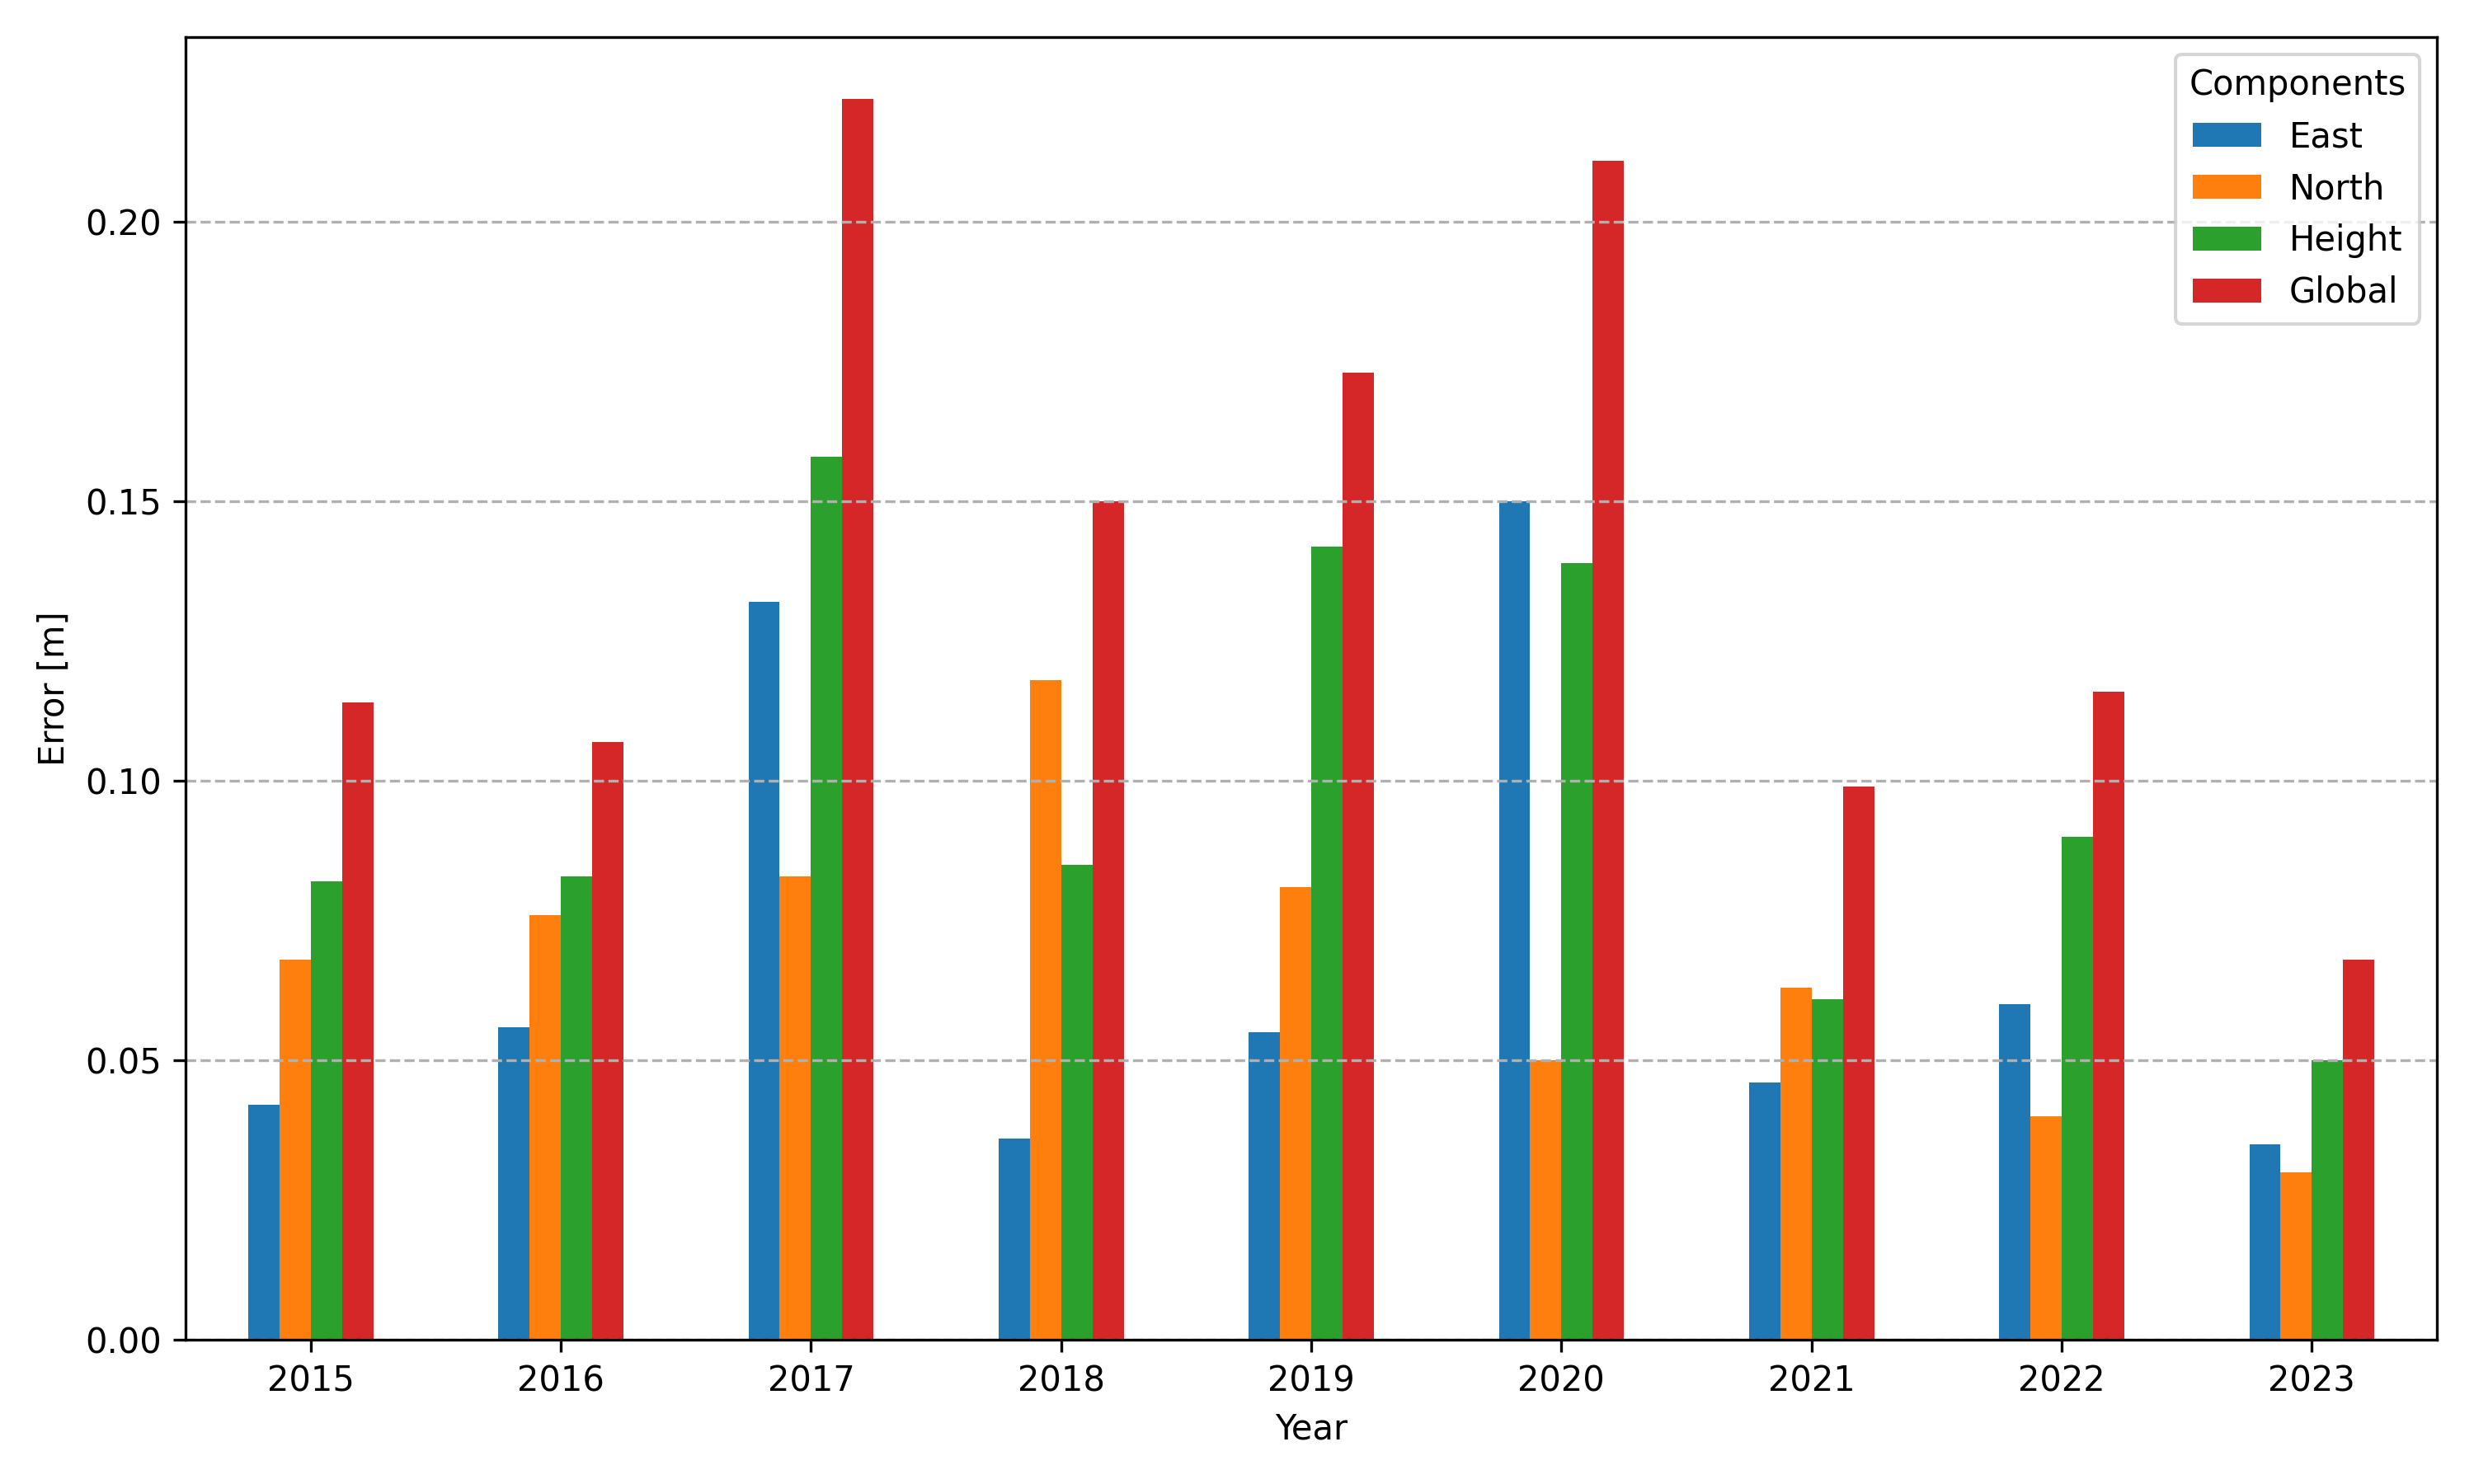
\includegraphics[width=0.9\columnwidth]{uav_cp_error.png}
    \caption{Barplot of reprojection RMSE computed on CPs for each photogrammetric
        model. Due to the technical problems that occurred in 2020 
        (see \secref{sec:3:problems}), the 2020 RMSE refers only to the survey of
        the lower part of the glacier, excluding the upper accumulation sector.
    }
    \label{fig:3:CP_errors}
\end{figure}

\begin{figure}
    \centering
    \subcaptionbox{\label{fig:3:ortophoto:2015}}{
        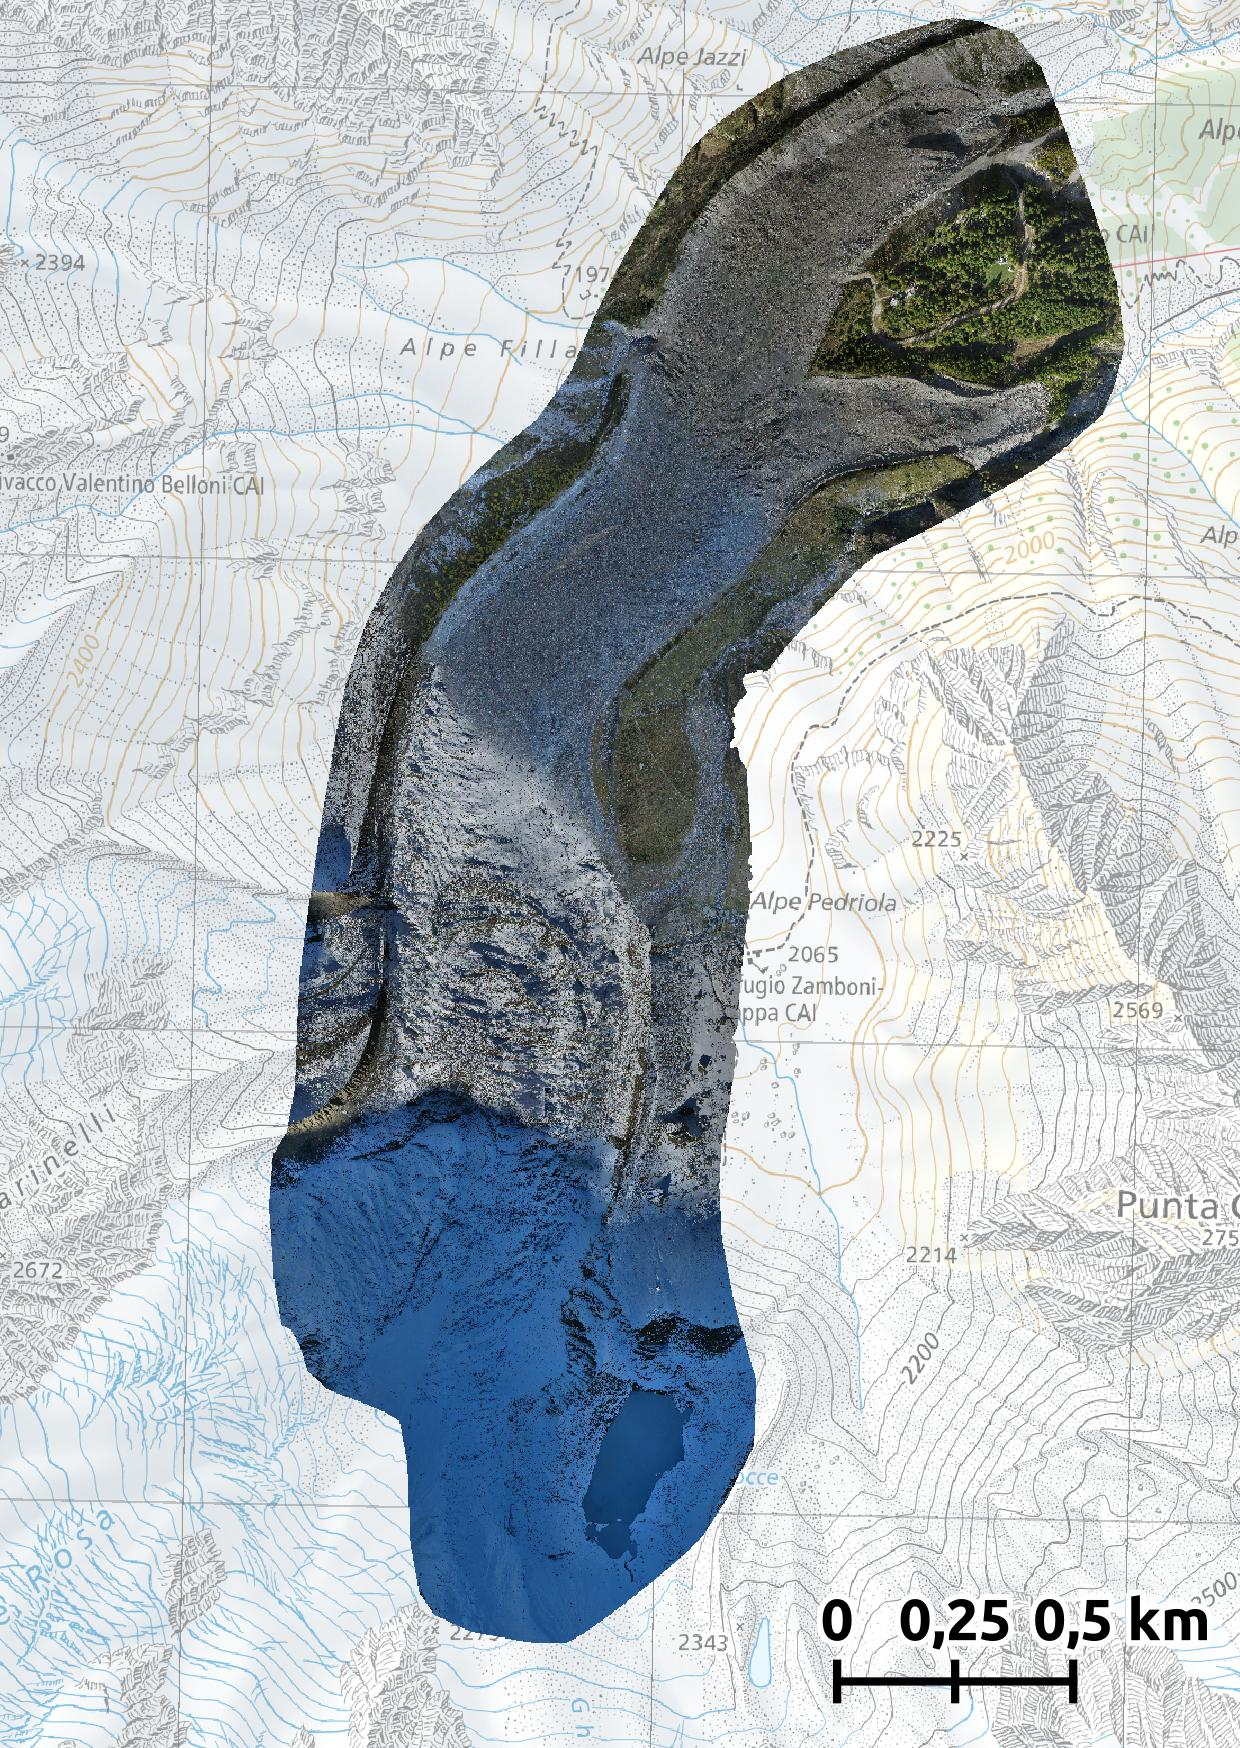
\includegraphics[width=0.25\textwidth]{orto2015.jpg}
    }
    \subcaptionbox{\label{fig:3:ortophoto:2016}}{
        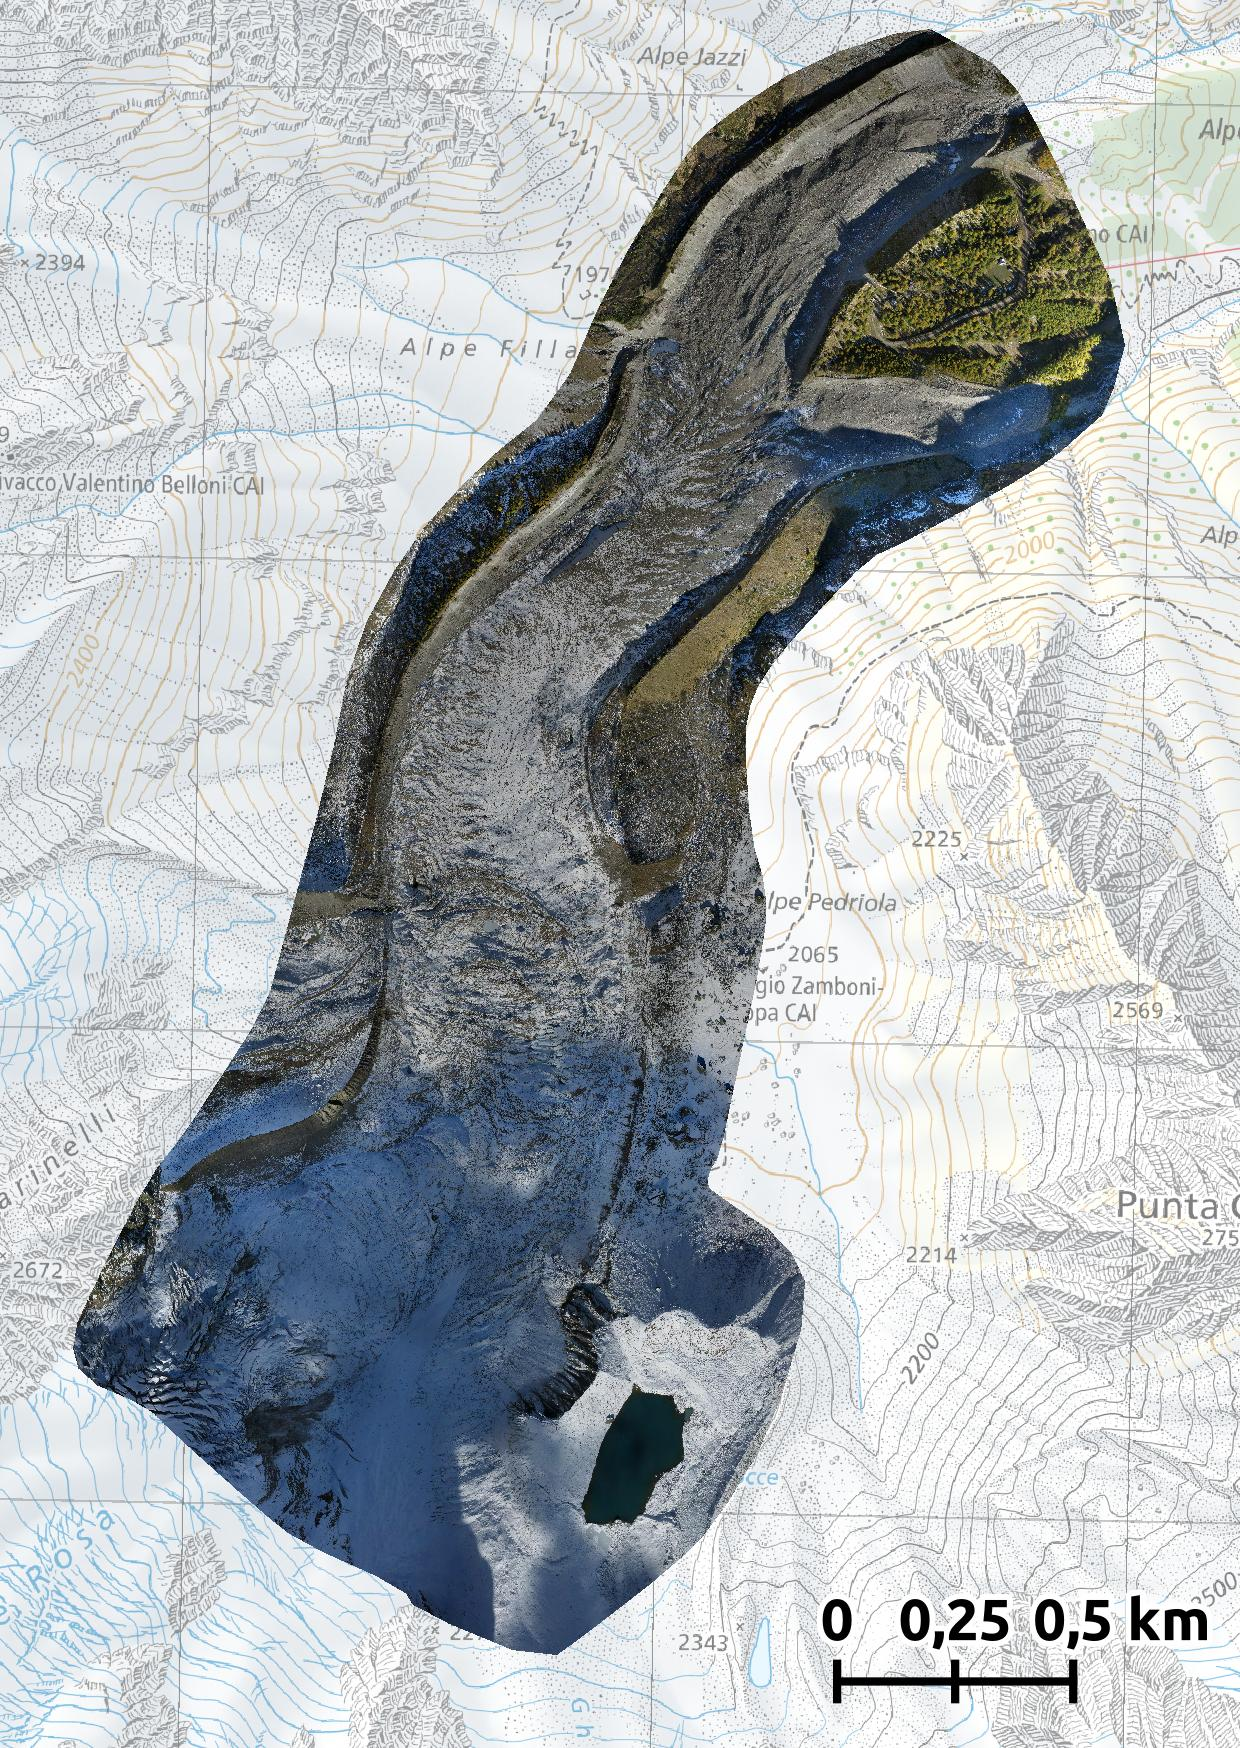
\includegraphics[width=0.25\textwidth]{orto2016.jpg}
    }
    \subcaptionbox{\label{fig:3:ortophoto:2017}}{
        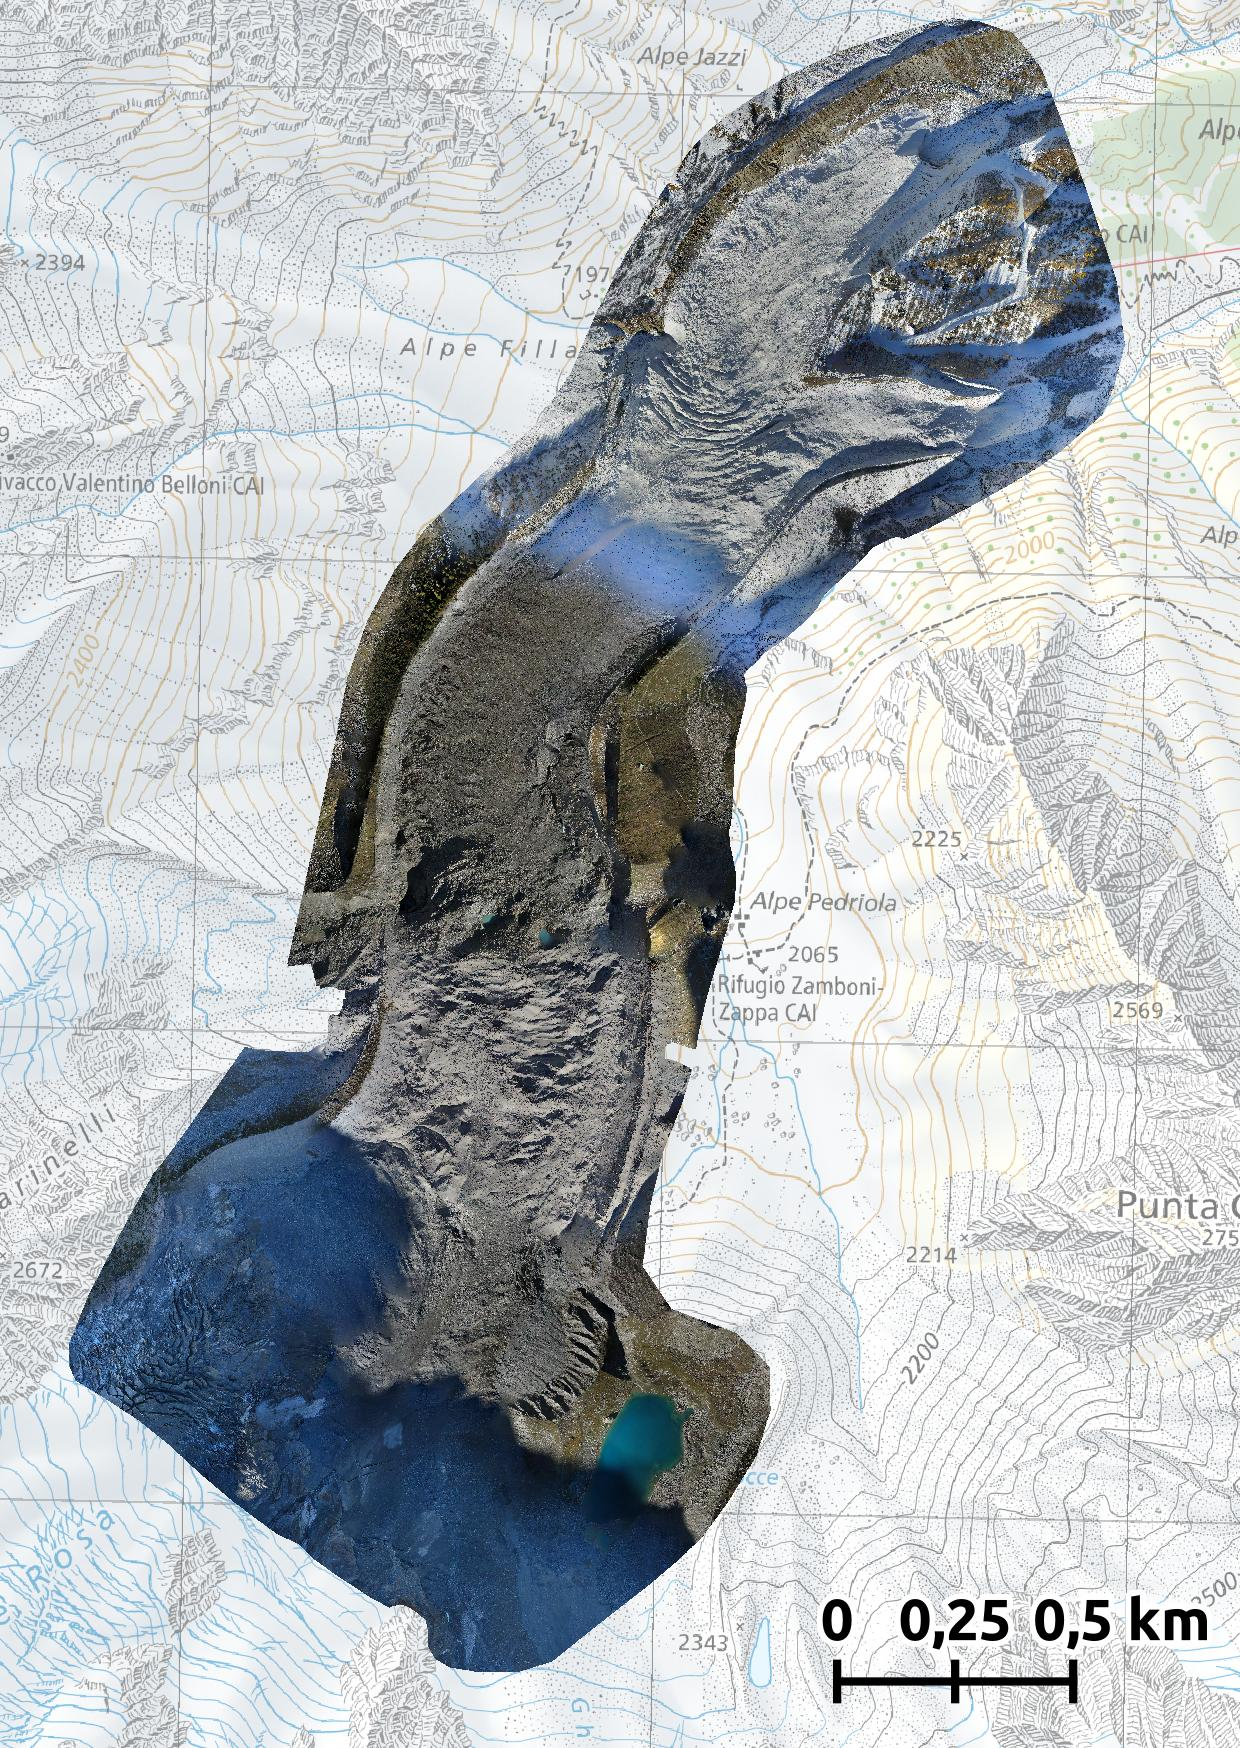
\includegraphics[width=0.25\textwidth]{orto2017.jpg}
    }
    \\
    \subcaptionbox{\label{fig:3:ortophoto:2018}}{
        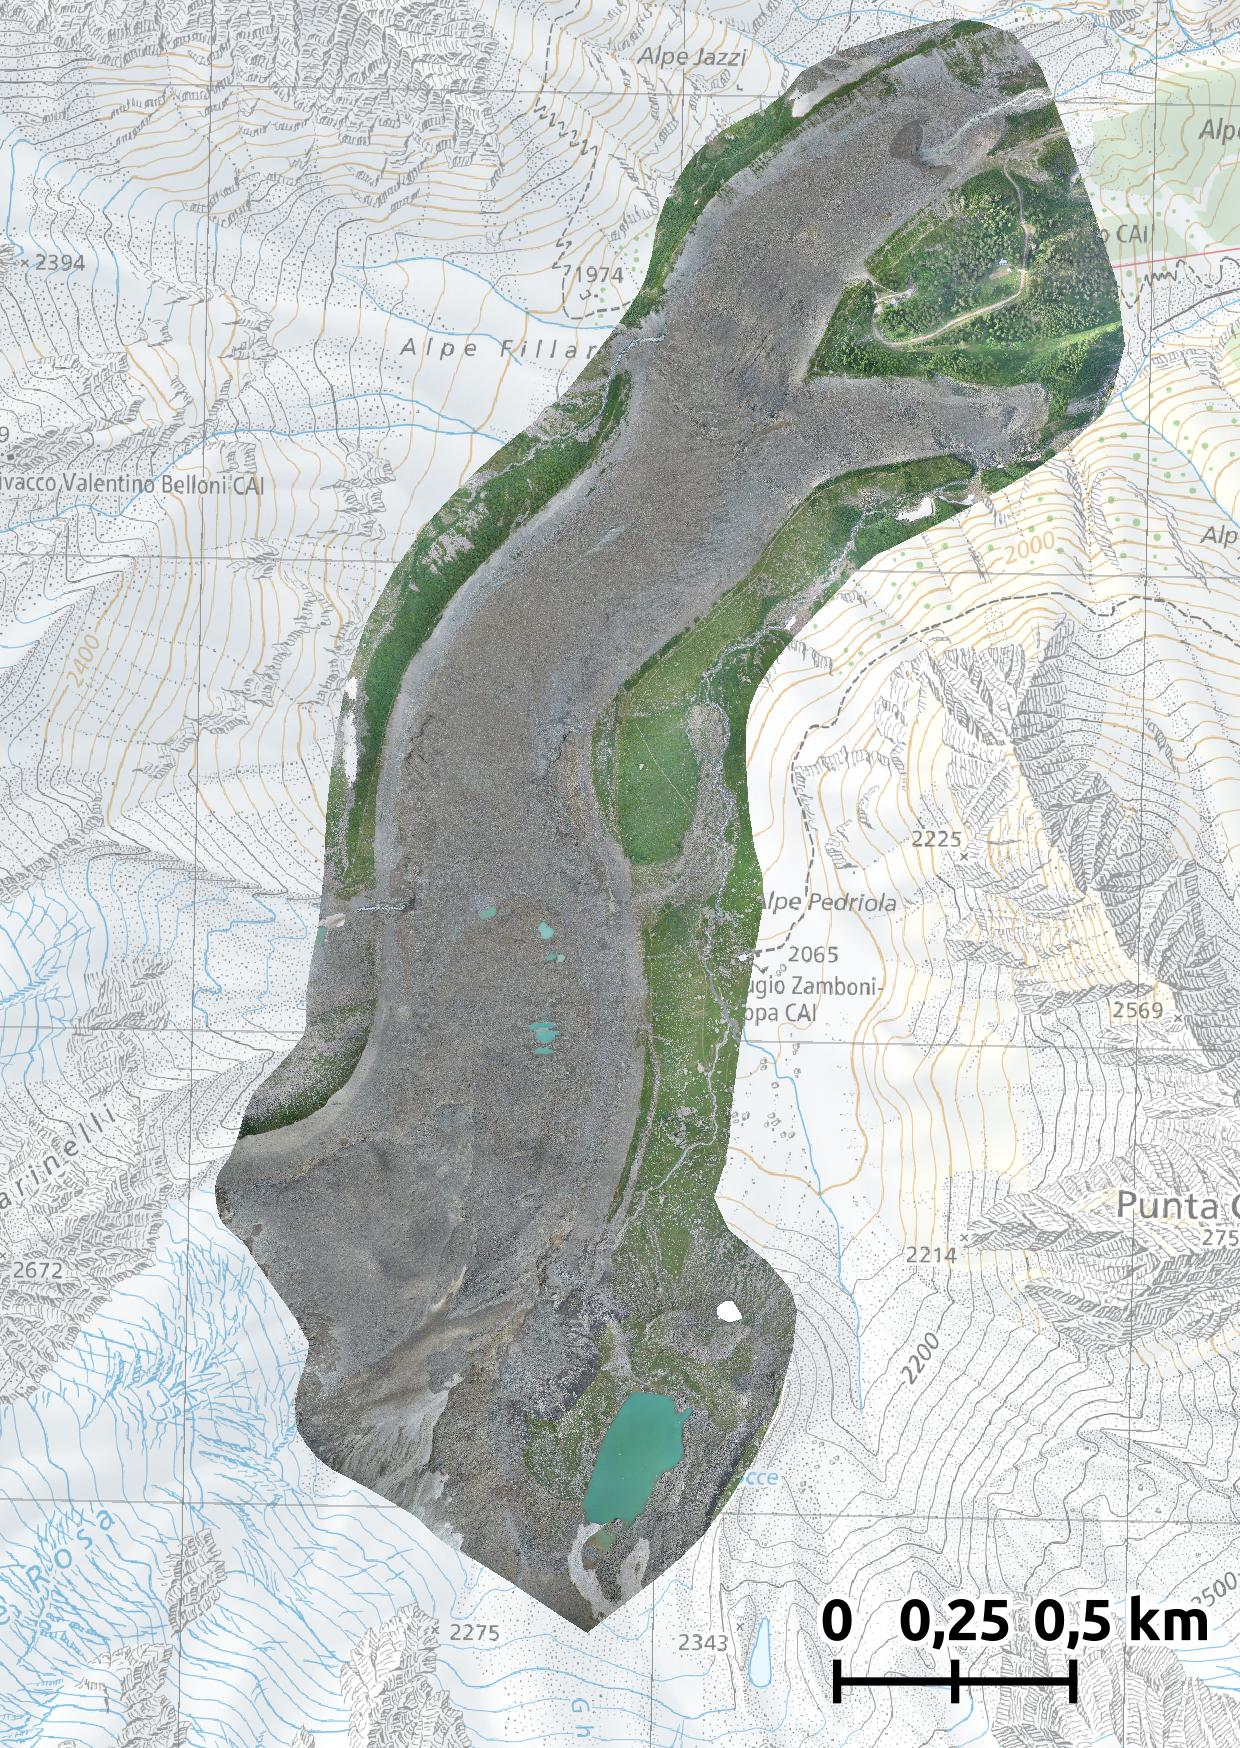
\includegraphics[width=0.25\textwidth]{orto2018.jpg}
    }
    \subcaptionbox{\label{fig:3:ortophoto:2019}}{
        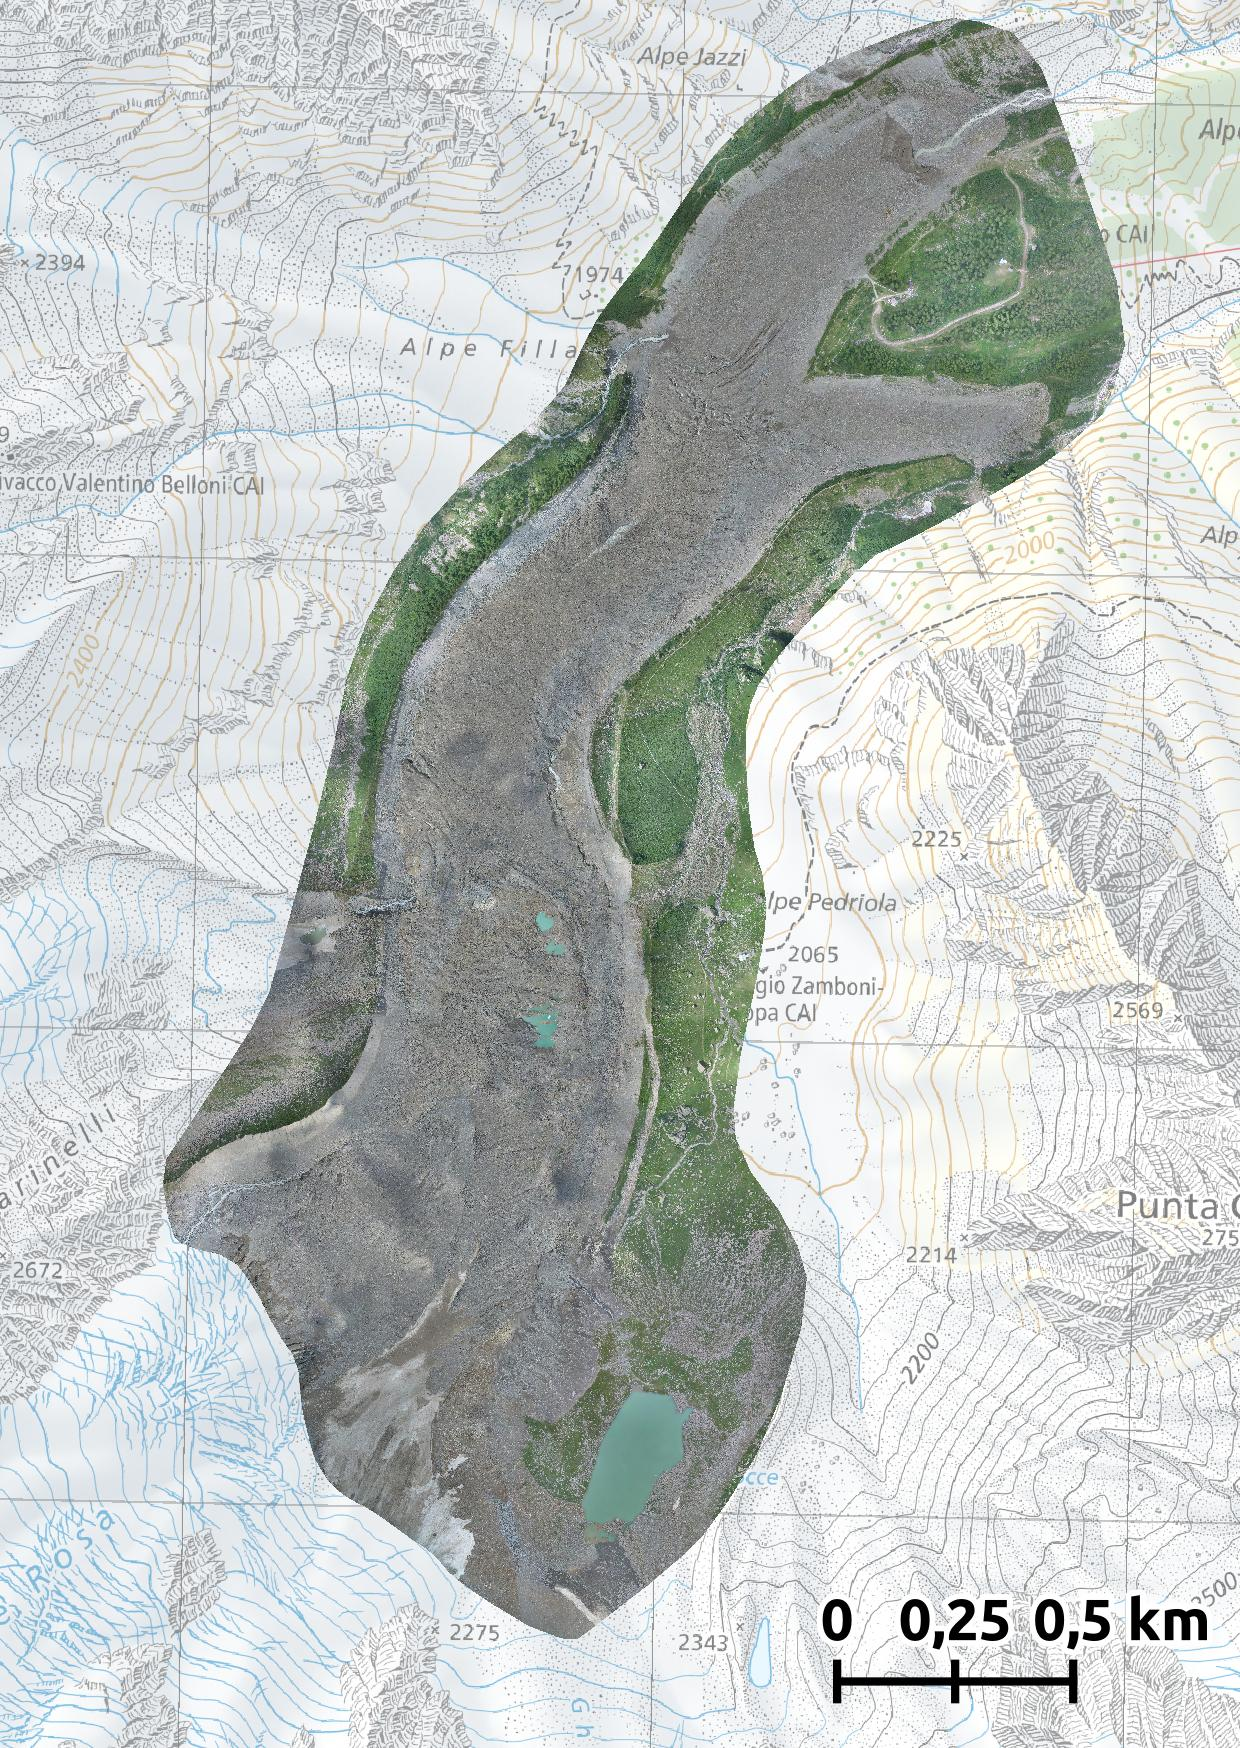
\includegraphics[width=0.25\textwidth]{orto2019.jpg}
    }
    \subcaptionbox{\label{fig:3:ortophoto:2020}}{
        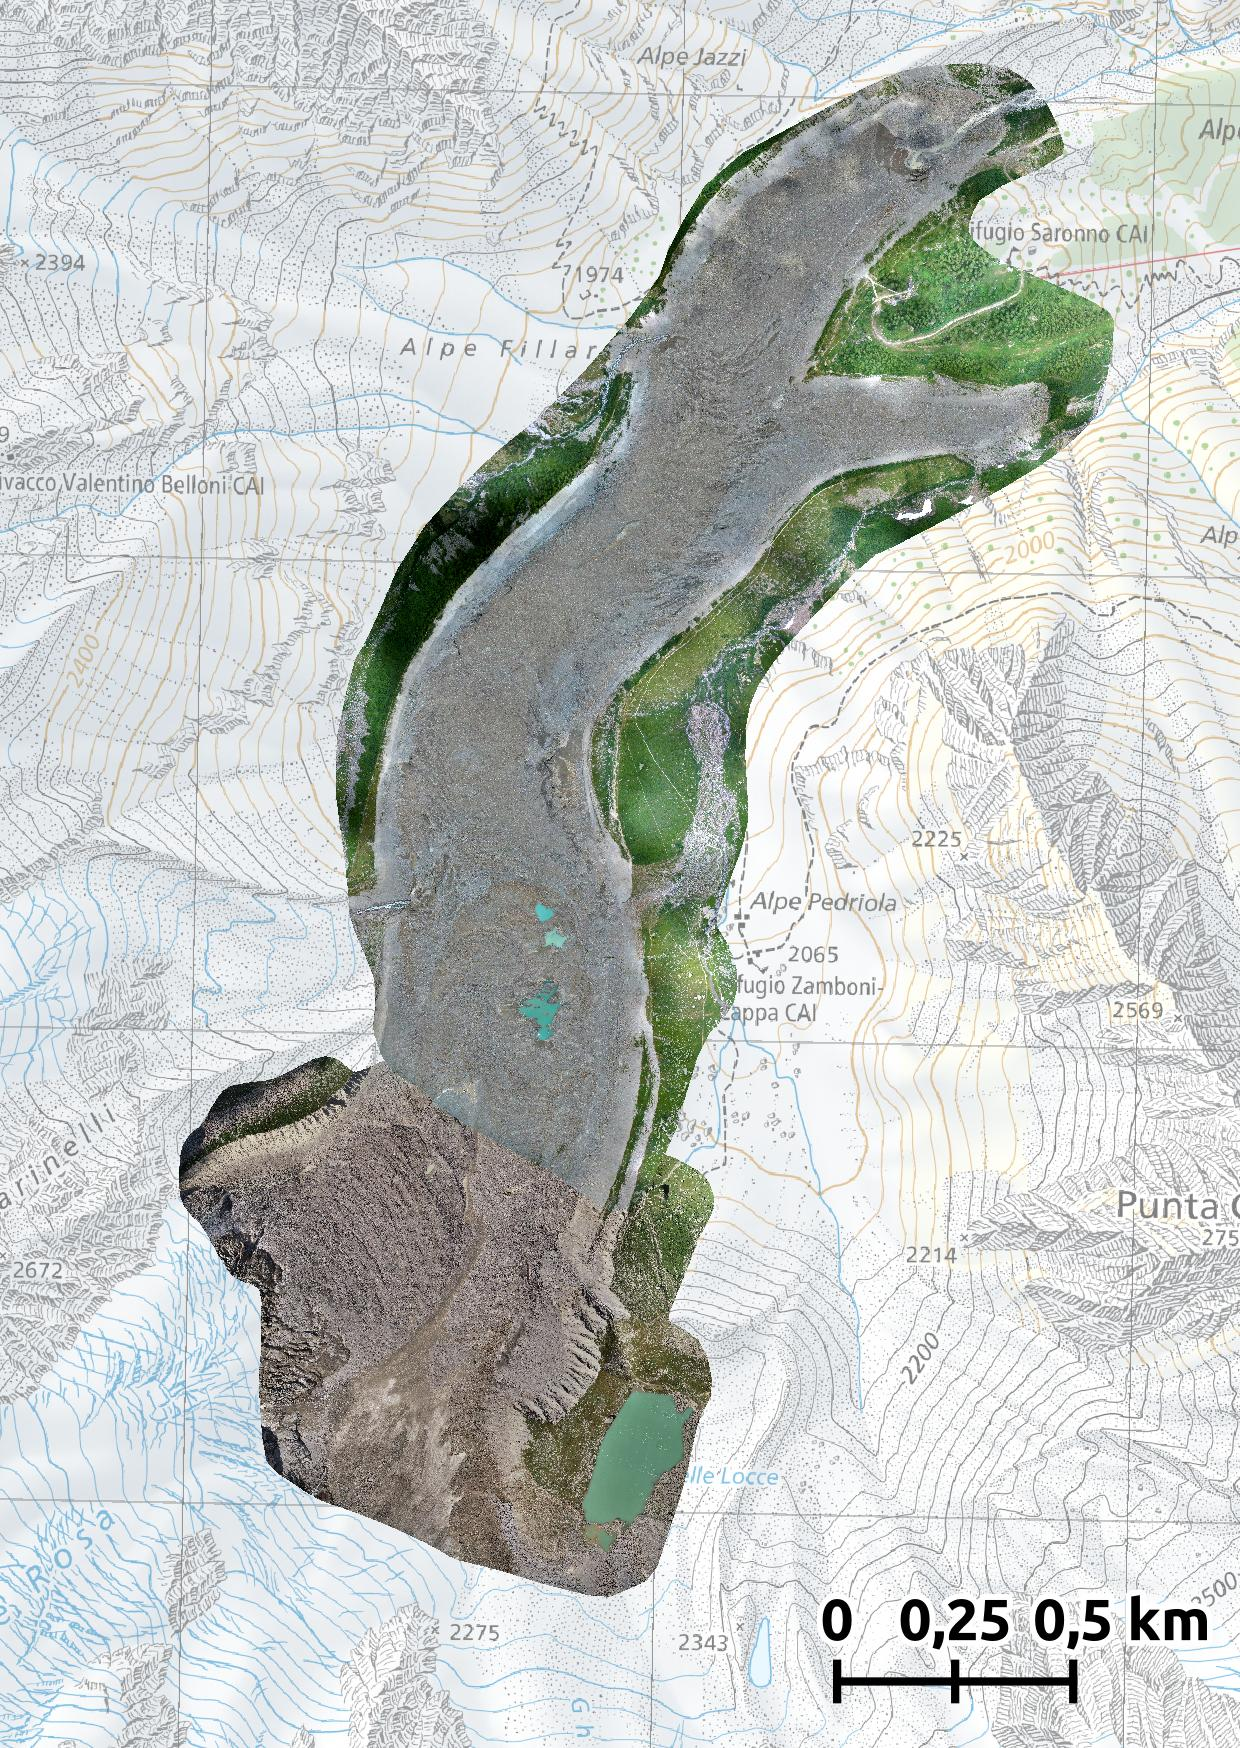
\includegraphics[width=0.25\textwidth]{orto2020.jpg}
    }
    \subcaptionbox{\label{fig:3:ortophoto:2021}}{
        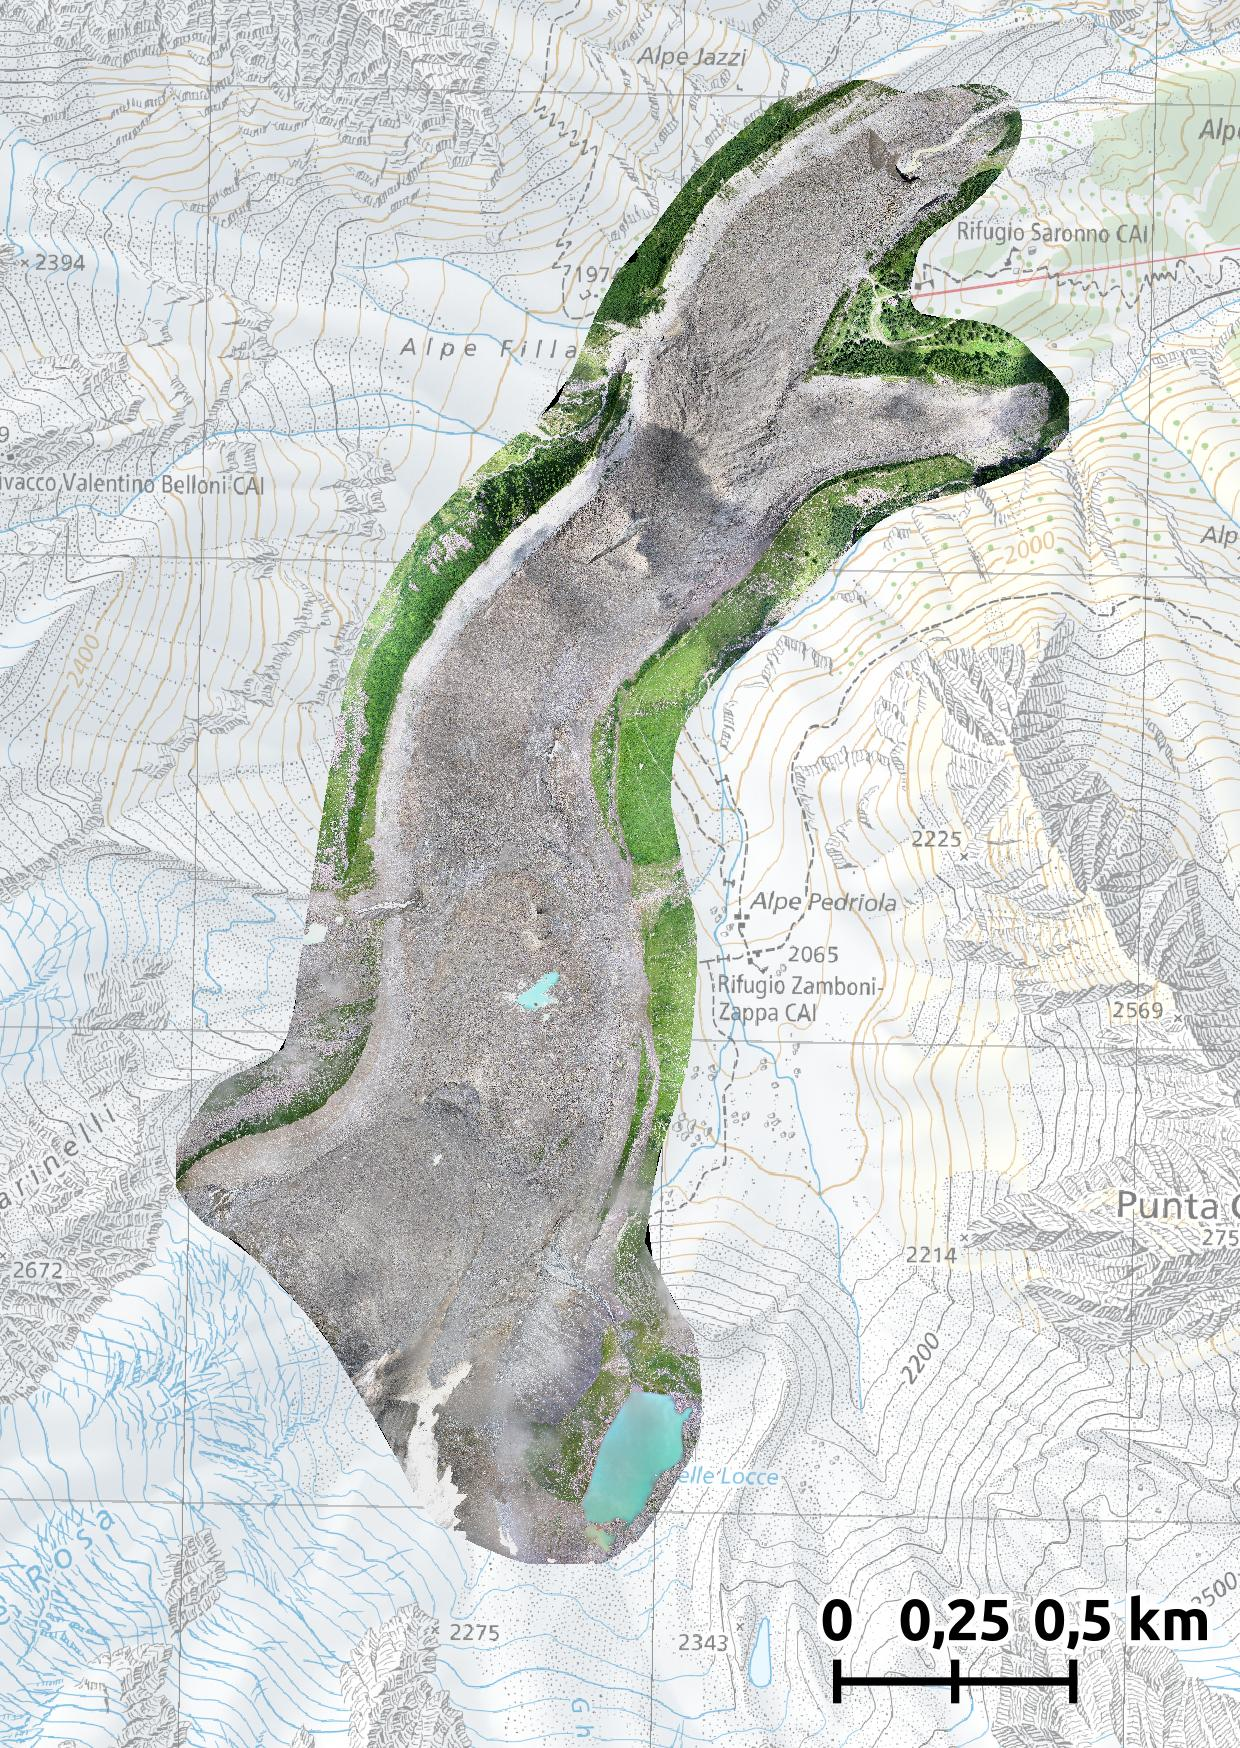
\includegraphics[width=0.25\textwidth]{orto2021.jpg}
    }
    \subcaptionbox{\label{fig:3:ortophoto:2022}}{
        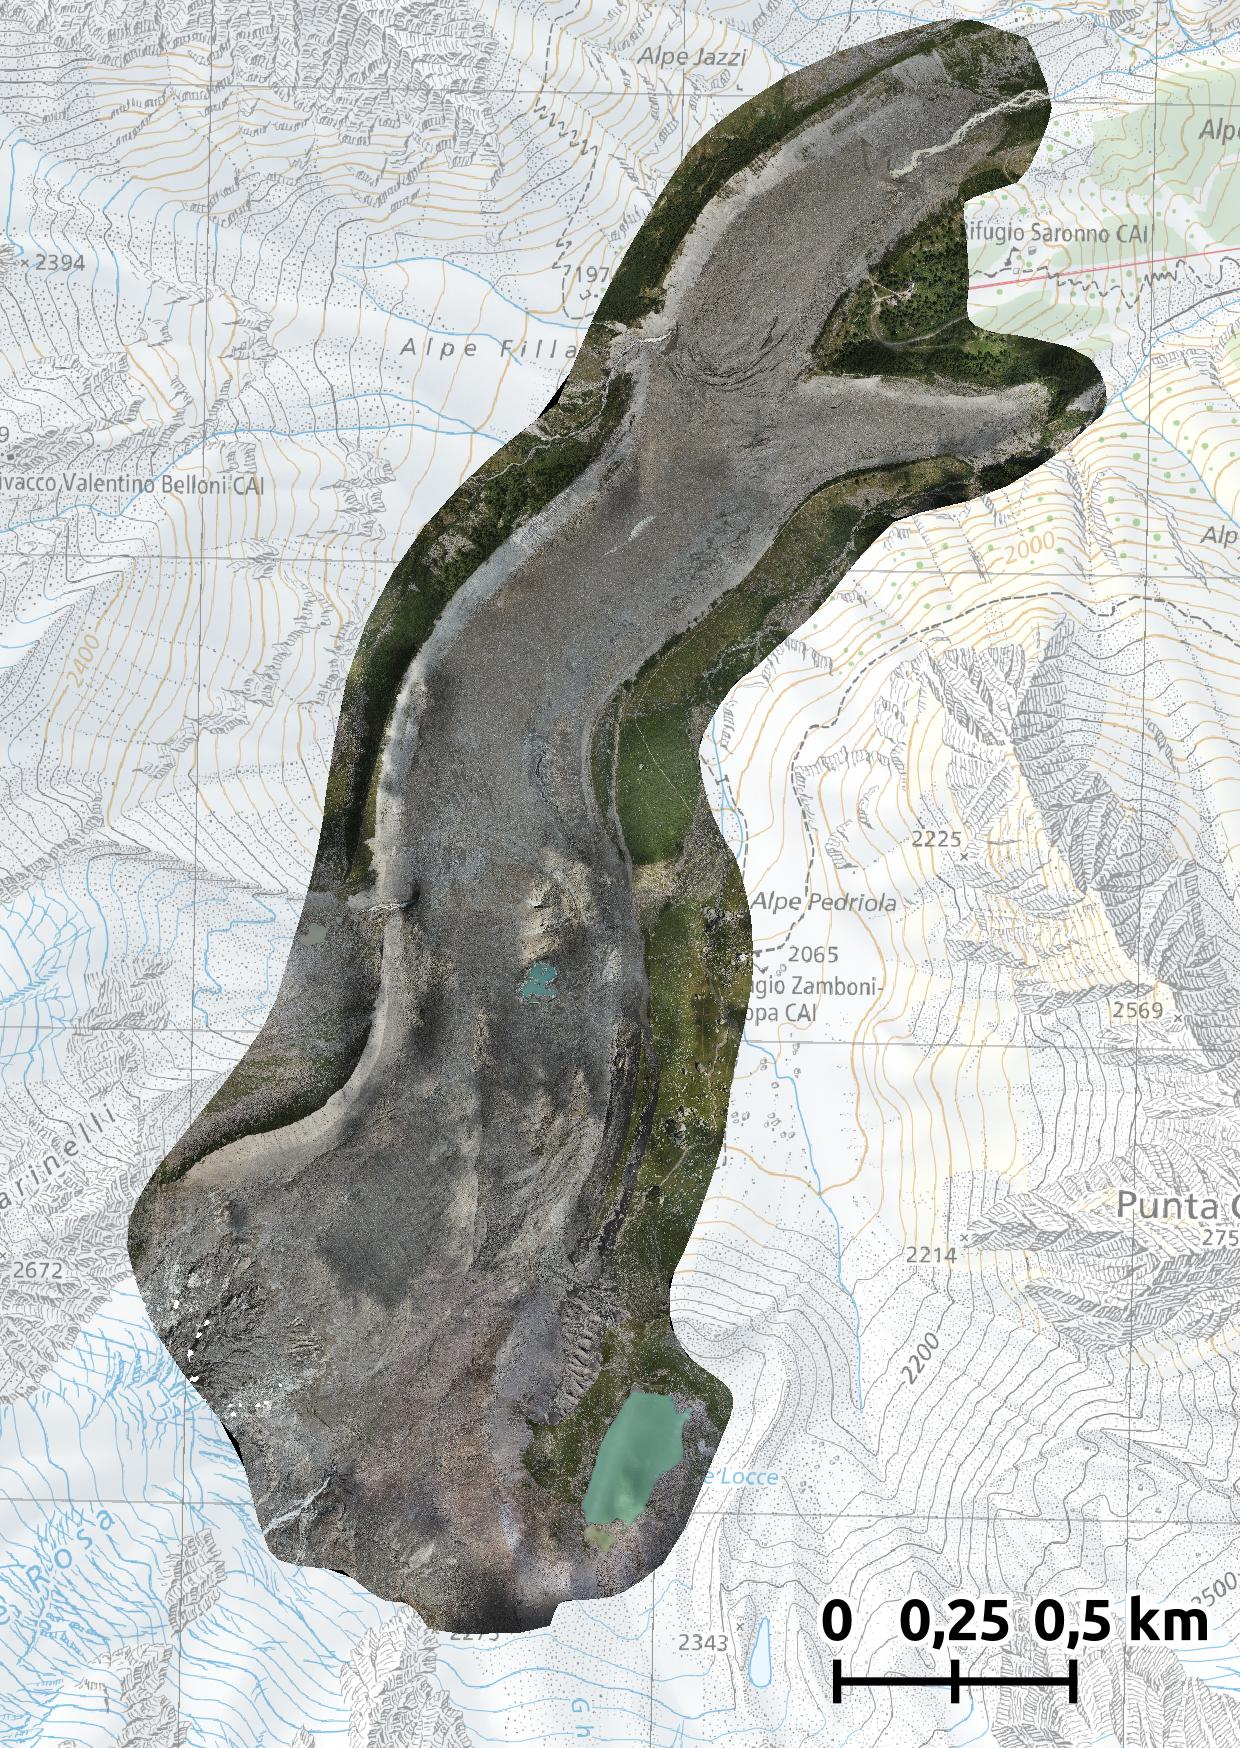
\includegraphics[width=0.25\textwidth]{orto2022.jpg}
    }
    \subcaptionbox{\label{fig:3:ortophoto:2023}}{
        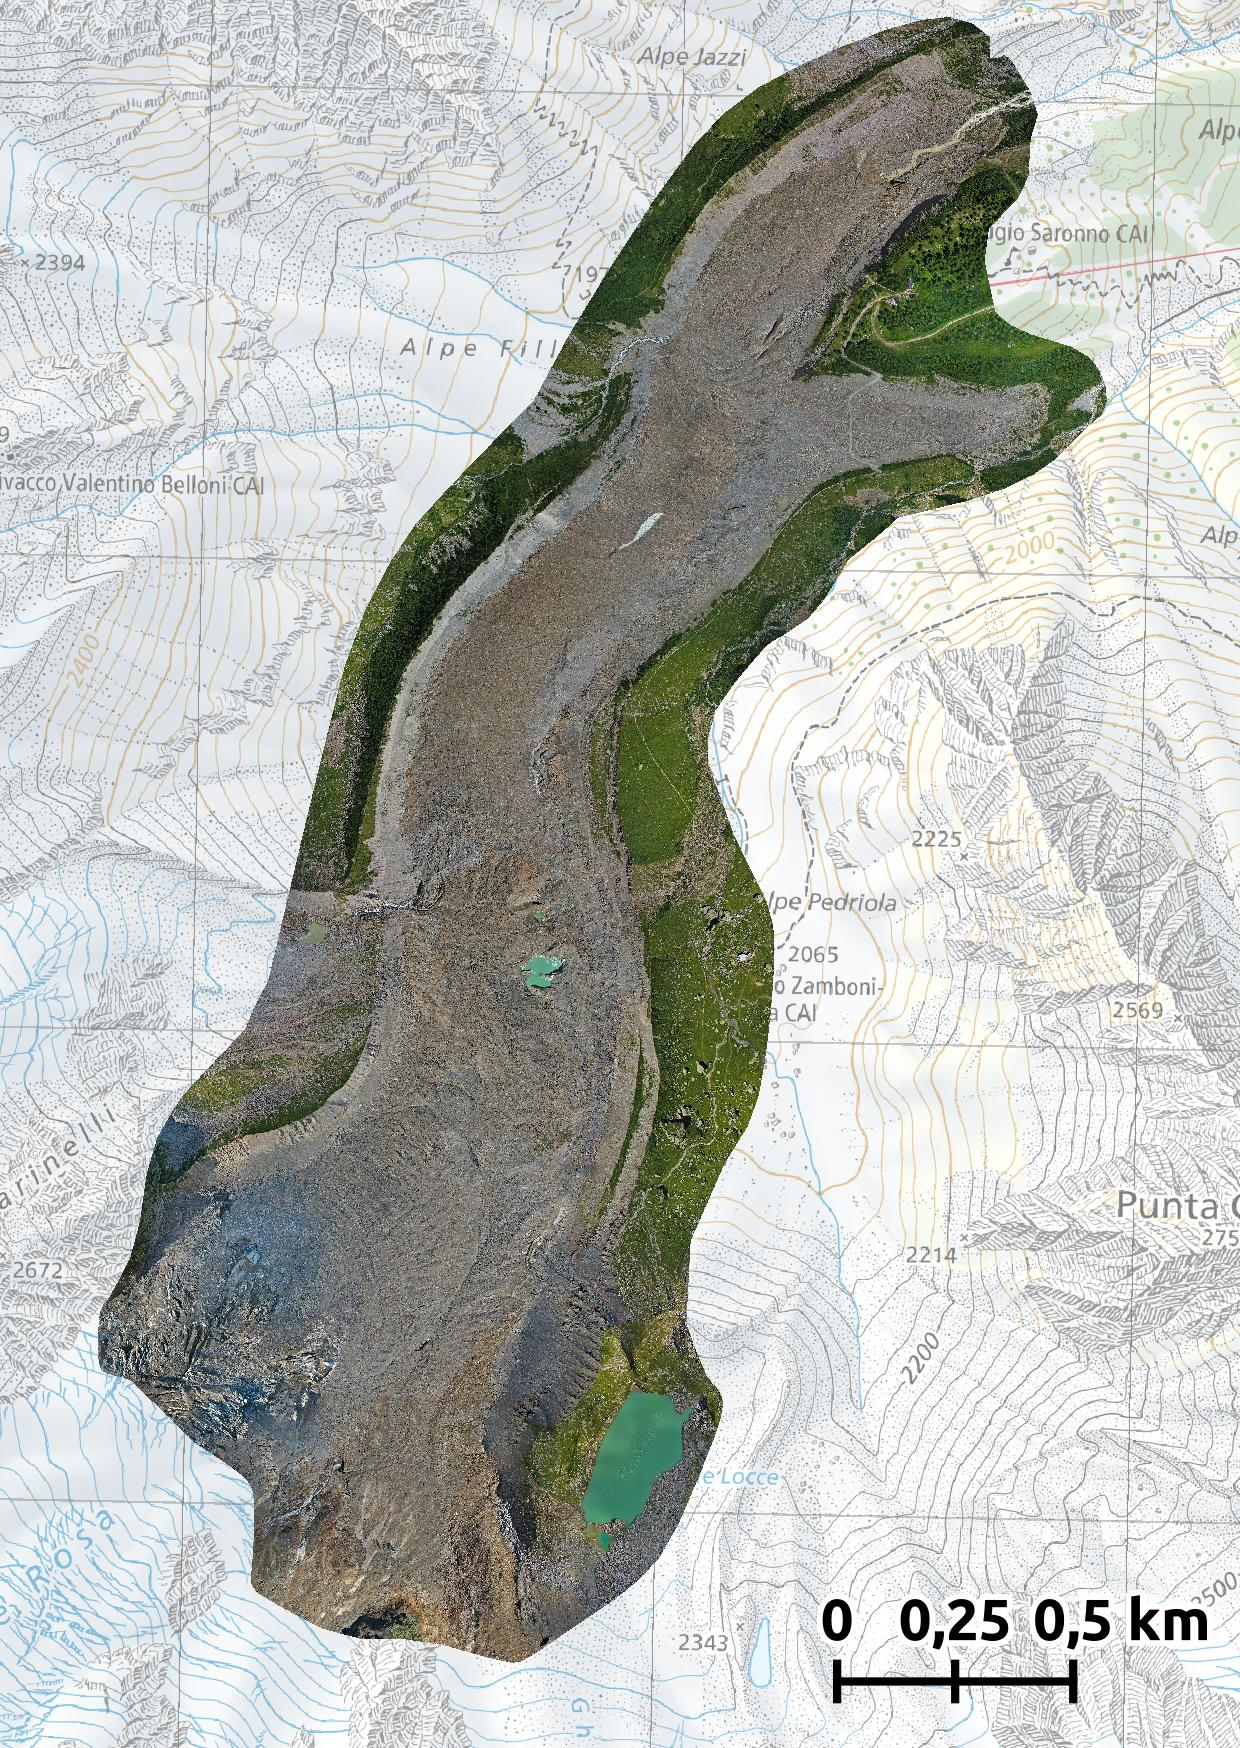
\includegraphics[width=0.25\textwidth]{orto2023.jpg}
    }
    \caption{Orthophotos obtained from the photogrammetric model for each year.
        (\textbf{a}) 2015, (\textbf{b}) 2016, (\textbf{c}) 2017, (\textbf{d}) 2018,
        (\textbf{e}) 2019, (\textbf{f}) 2020, (\textbf{g}) 2021, (\textbf{h}) 2022, (\textbf{i}) 2023. Orthophotos are overlapped to the Swisstopo base map (source: Swisstopo www.geo.admin.ch). Refer to the Appendix \ref{app:orthophotos} for a better visualization of the orthophotos.}
    \label{fig:3:ortophoto}
\end{figure}

\section{Results}\label{sec:3:res}

\subsection{SfM}\label{sec:3:res:sfm}

Each SfM process yielded a 3D point cloud, a textured mesh, a DSM, and an orthophoto of the glacier. 
Point cloud density increased over time: point clouds from 2015 to 2020 contained \SI{0.5e8}{} to \SI{1e8}{} 
points, while those from 2021 onwards had \SI{1.5e8}{} to \SI{2.5e8}{} points. 
DSMs and orthophotos were produced at a resolution of 20 centimeters per pixel.
Due to autumn surveys, orthophotos from 2015 to 2017 show some snow cover (\figref{fig:3:ortophoto}).

The geometrical accuracy of the SfM models was evaluated for all years using CPs.
\figref{fig:3:CP_errors} RMSE of on-ground error in all three directions and globally. 
RMSE values range between 0.1 m and 0.2 m across all years. 
Note that for 2020, errors reflect the lower part of the glacier only, as the upper part was
surveyed with a separate photogrammetric flight that lacked GNSS-measured GCPs but relied on
natural features identified in the 2019 model as GCPs (see \secref{sec:3:problems}).

% From 2015 to 2017, when compact cameras were used, errors smaller than 2 times the GSD
% were obtained.
% From 2018 to 2020, a lightweight action cam has been employed to minimize the UAV take-off
% weight and this has led to an RMSE up to 3~times the GSD but still always smaller than
% \SI{0.2}{\meter}.
% From 2021, errors smaller than 2 times the GSD
% accuracy from 1 to 1.5 times the GSD.

\subsection{Glacier flow velocity}\label{sec:3:res:velocity}

\begin{figure}[ht!]
    \subcaptionbox{\label{fig:3:GNSS_velocity:ts}}{
        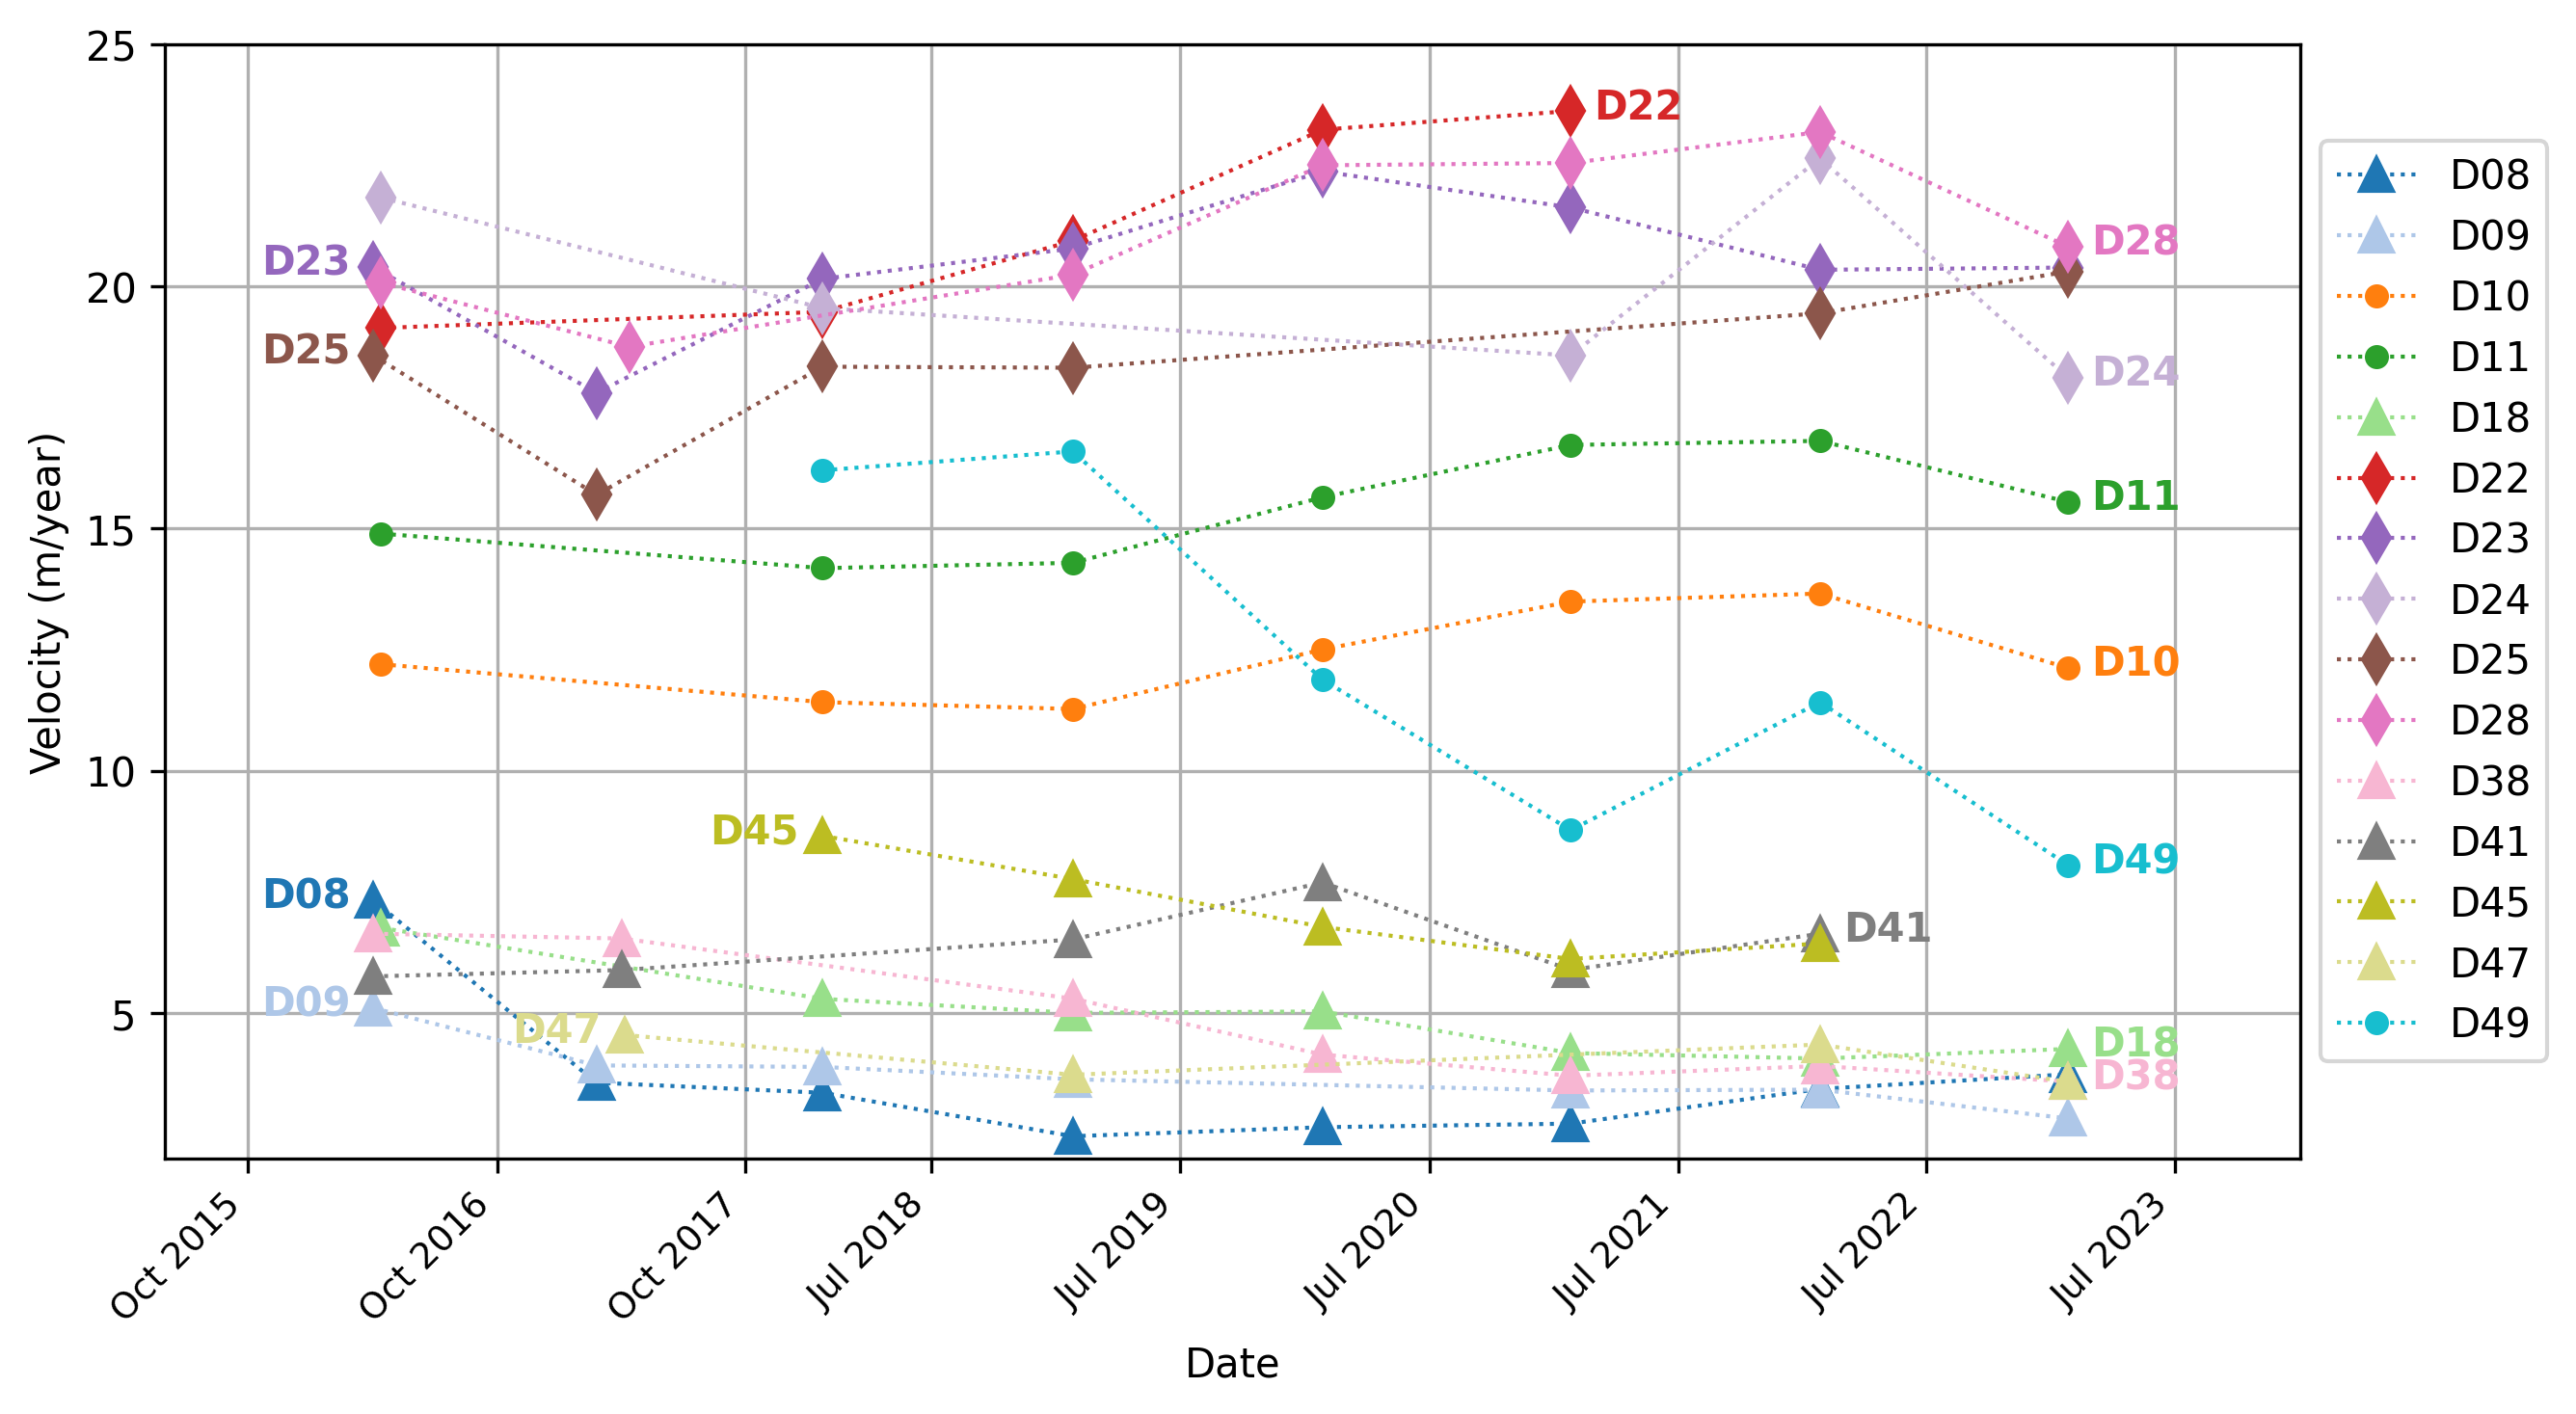
\includegraphics[height=6cm]{gnss_velocities}
    }
    \subcaptionbox{\label{fig:3:GNSS_velocity:map}}{
        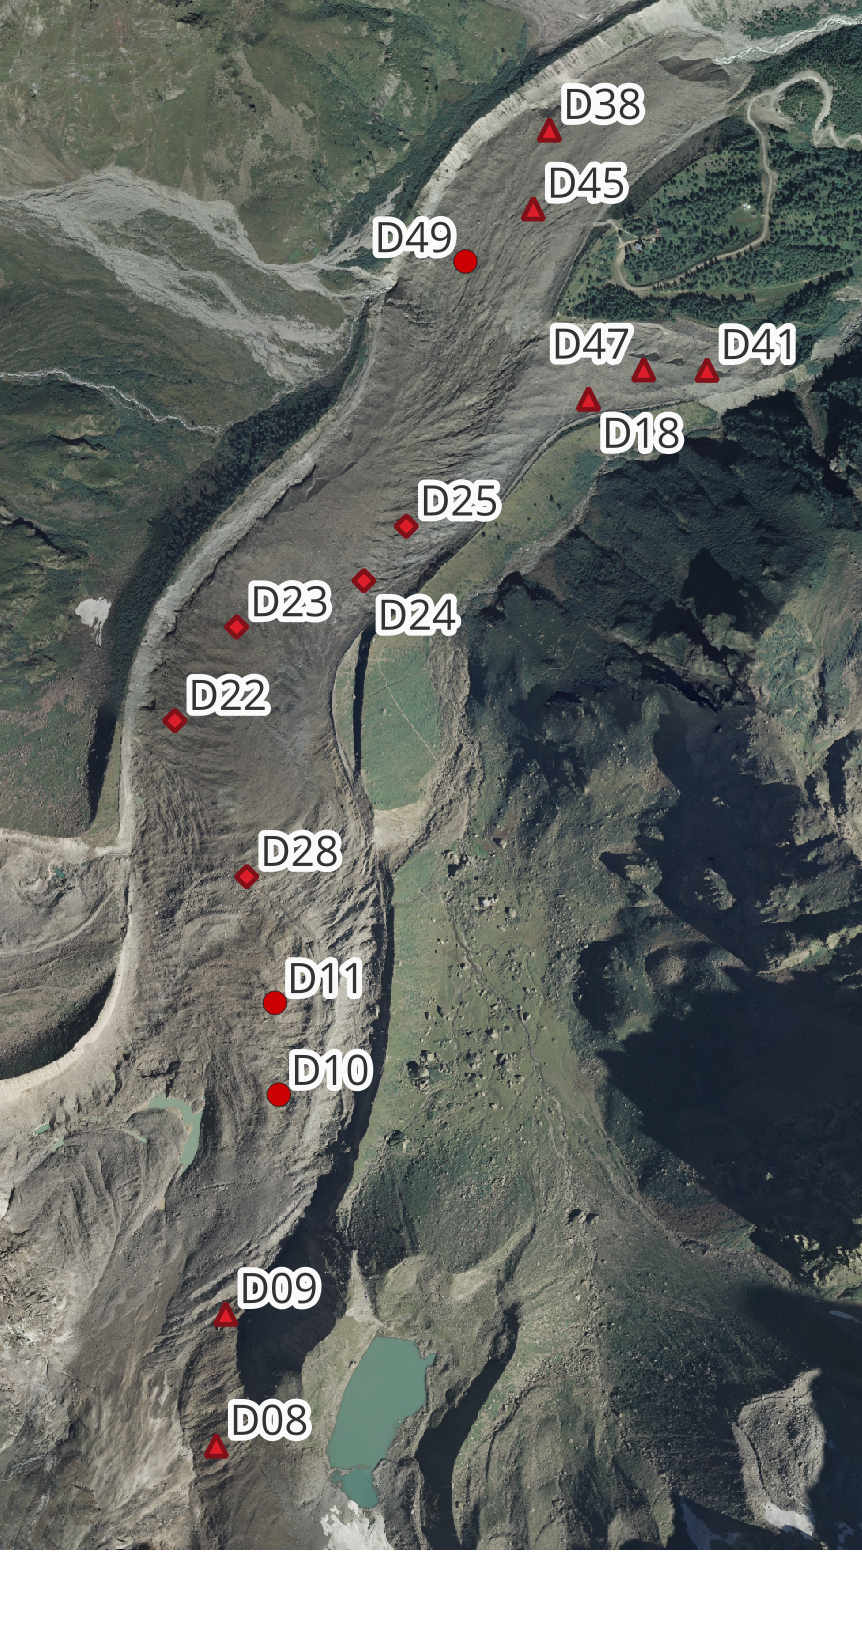
\includegraphics[height=6cm]{gnss_velocities_map}
    }
    \caption{\textbf{(a)} Time series of the velocity computed from the GNSS measurements of the targets deployed across the glacier. 
    \textbf{(b)} Location of the targets in the last surveying year.}
    \label{fig:3:GNSS_velocity}		
\end{figure}

Annual ice flow velocities were first computed using in-situ GNSS measurements of moving targets (\figref{fig:3:GNSS_velocity}).
Most of the moving targets were found and measured for three more years, and some of them have been continuously tracked since 2015 (e.g., \textit{M10}, \textit{M28}, \textit{M38}). 
While some targets were inevitably lost (e.g., due to the presence of crevasses), they were replaced with new ones materialized nearby to maintain data continuity. 

Analysis of the graph in \figref{fig:3:GNSS_velocity} reveals three distinct velocity clusters.  
The first cluster exhibits the lowest velocities ranging between \qtylist{2;8}{\meter\per\year} and encompasses points in the upper part of the glacier and glacier terminal lobes (e.g., targets \textit{M08, M09, M41, M45}). 
The glacier's central part is characterized by significantly faster speeds between \qtylist{16;25}{\meter\per\year} (e.g., targets \textit{M22, M23, M24, M25, M28}). 
The third cluster represents a transition zone with intermediate velocities found between the central sector and the upper accumulation area (targets \textit{M10, M11}) and between the central sector and the terminal lobes (e.g., target \textit{M49}).

\begin{figure}[!p]
    \centering
    \subcaptionbox{2015-2016\label{fig:3:dic_vel:2015}}{
        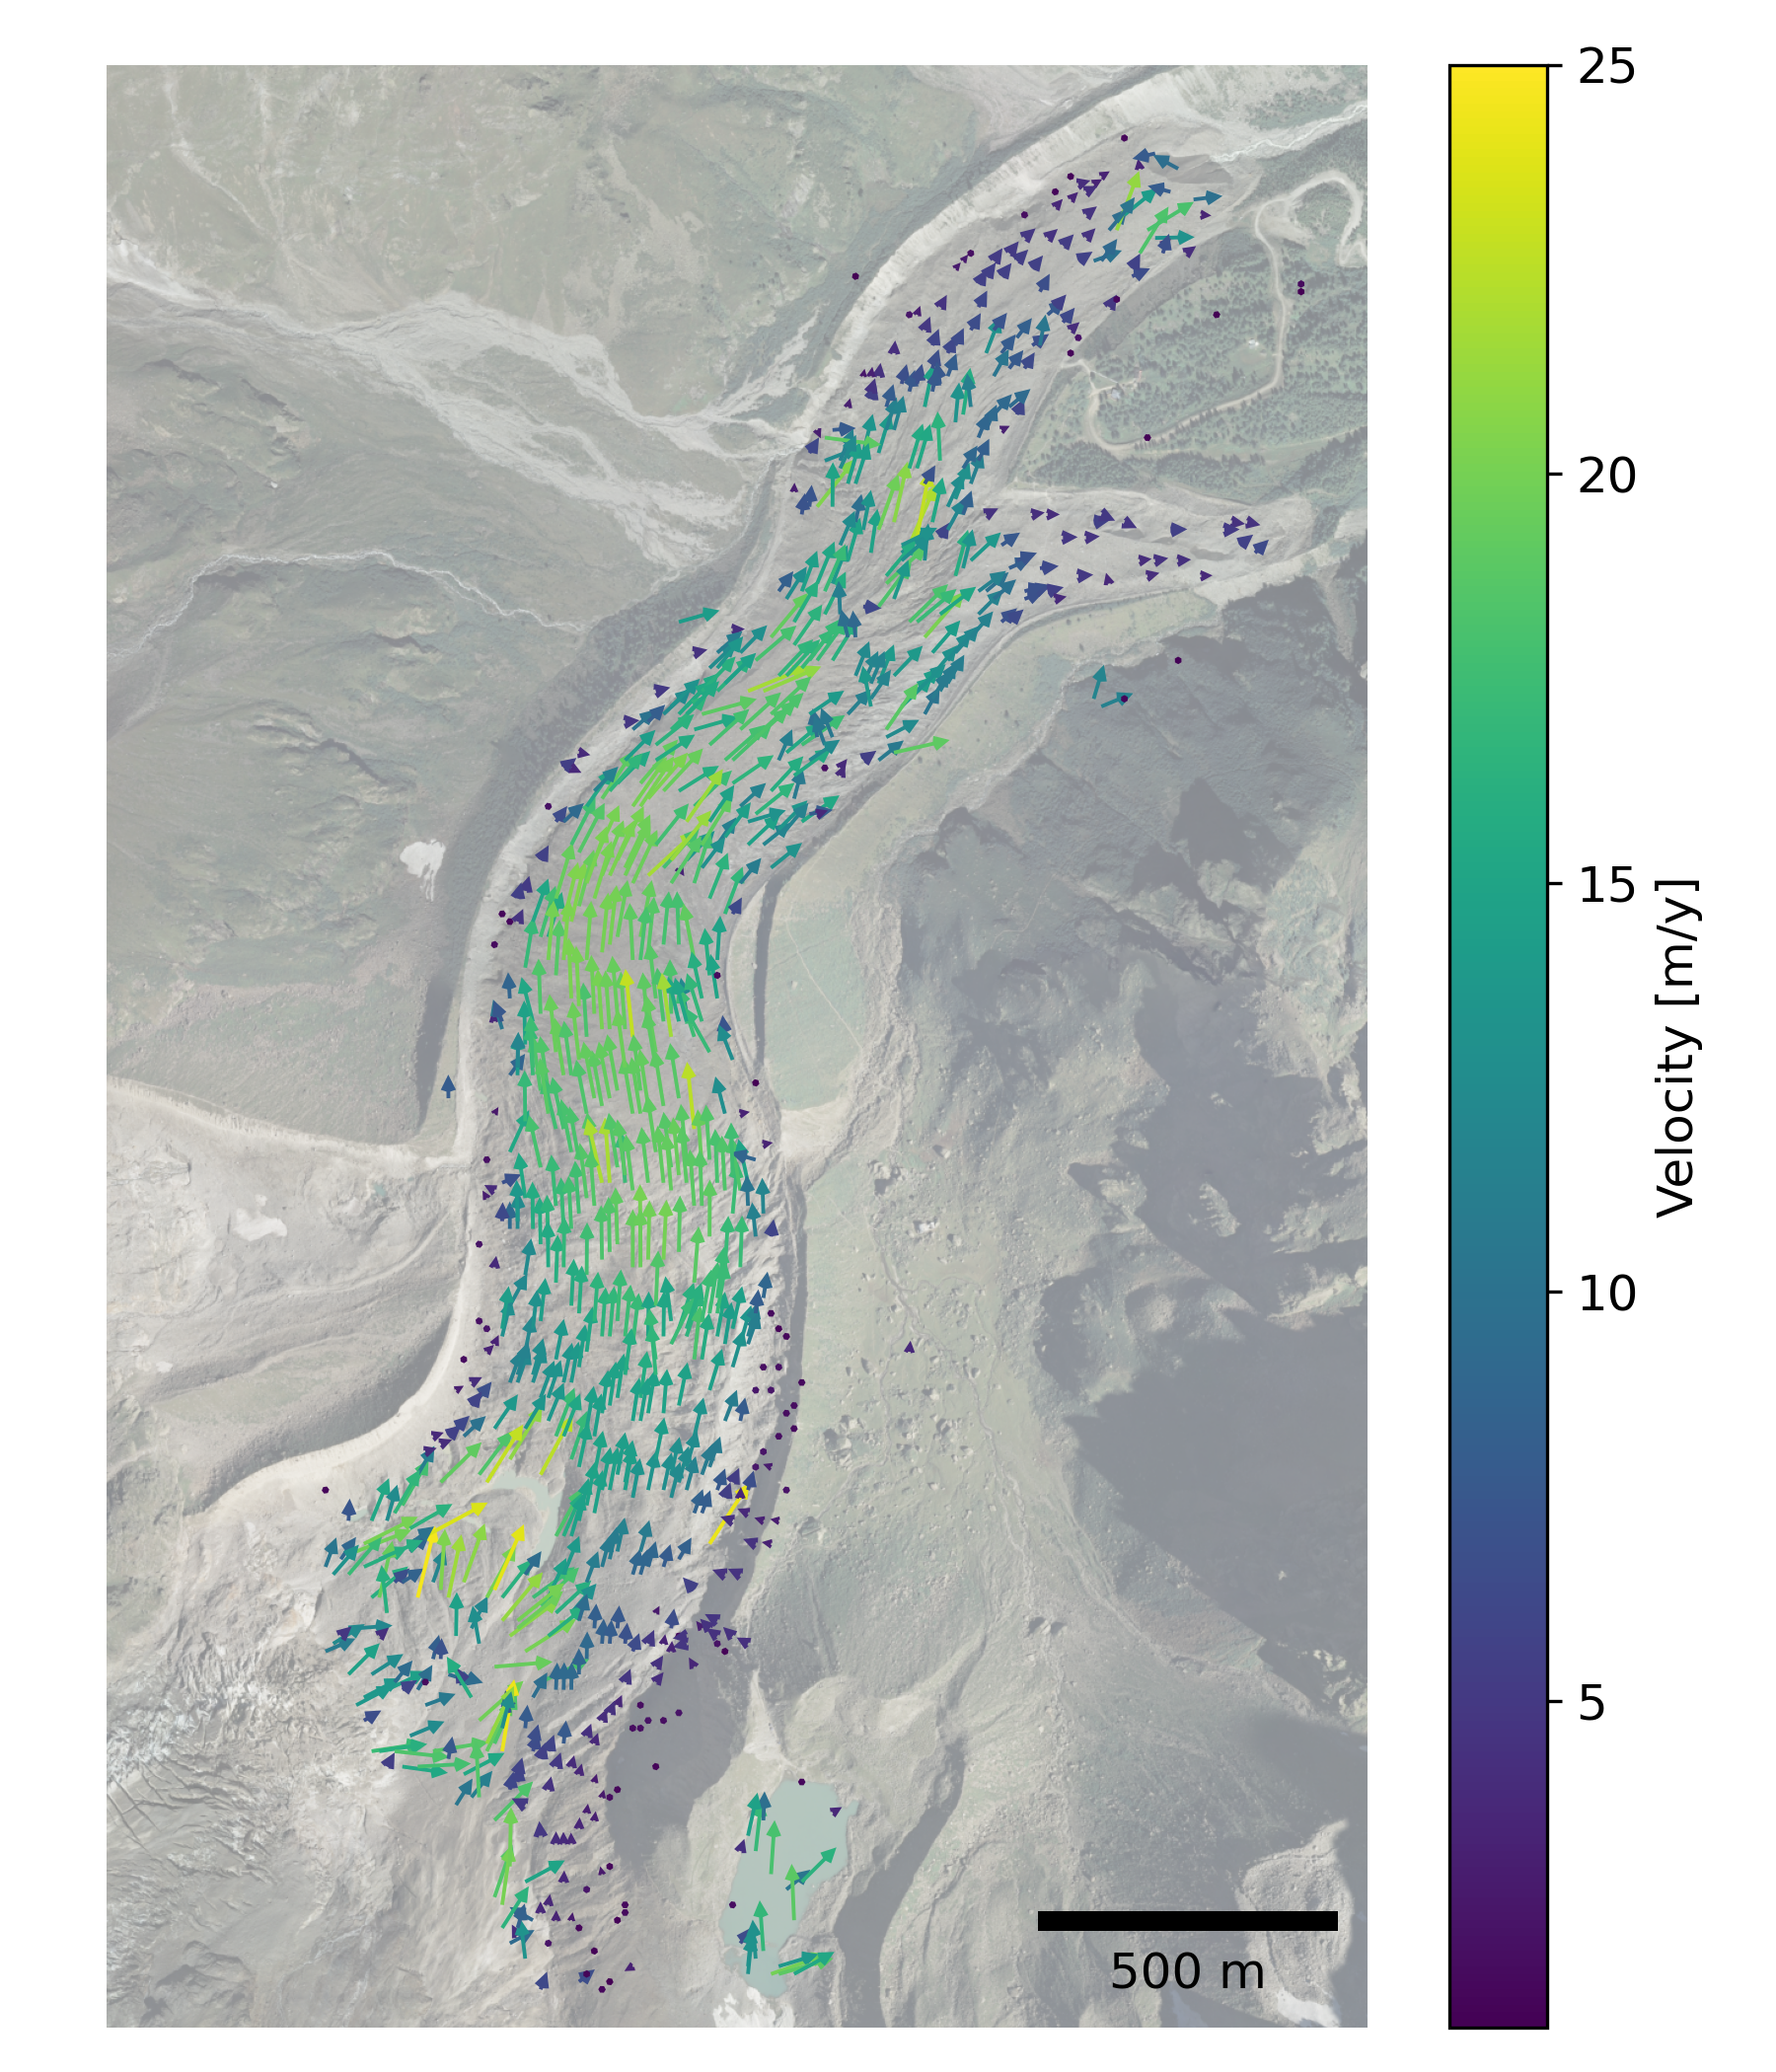
\includegraphics[width=0.44\textwidth]{velocity_DIC_2015-2016}
    }
    \subcaptionbox{2016-2017\label{fig:3:dic_vel:2016}}{
        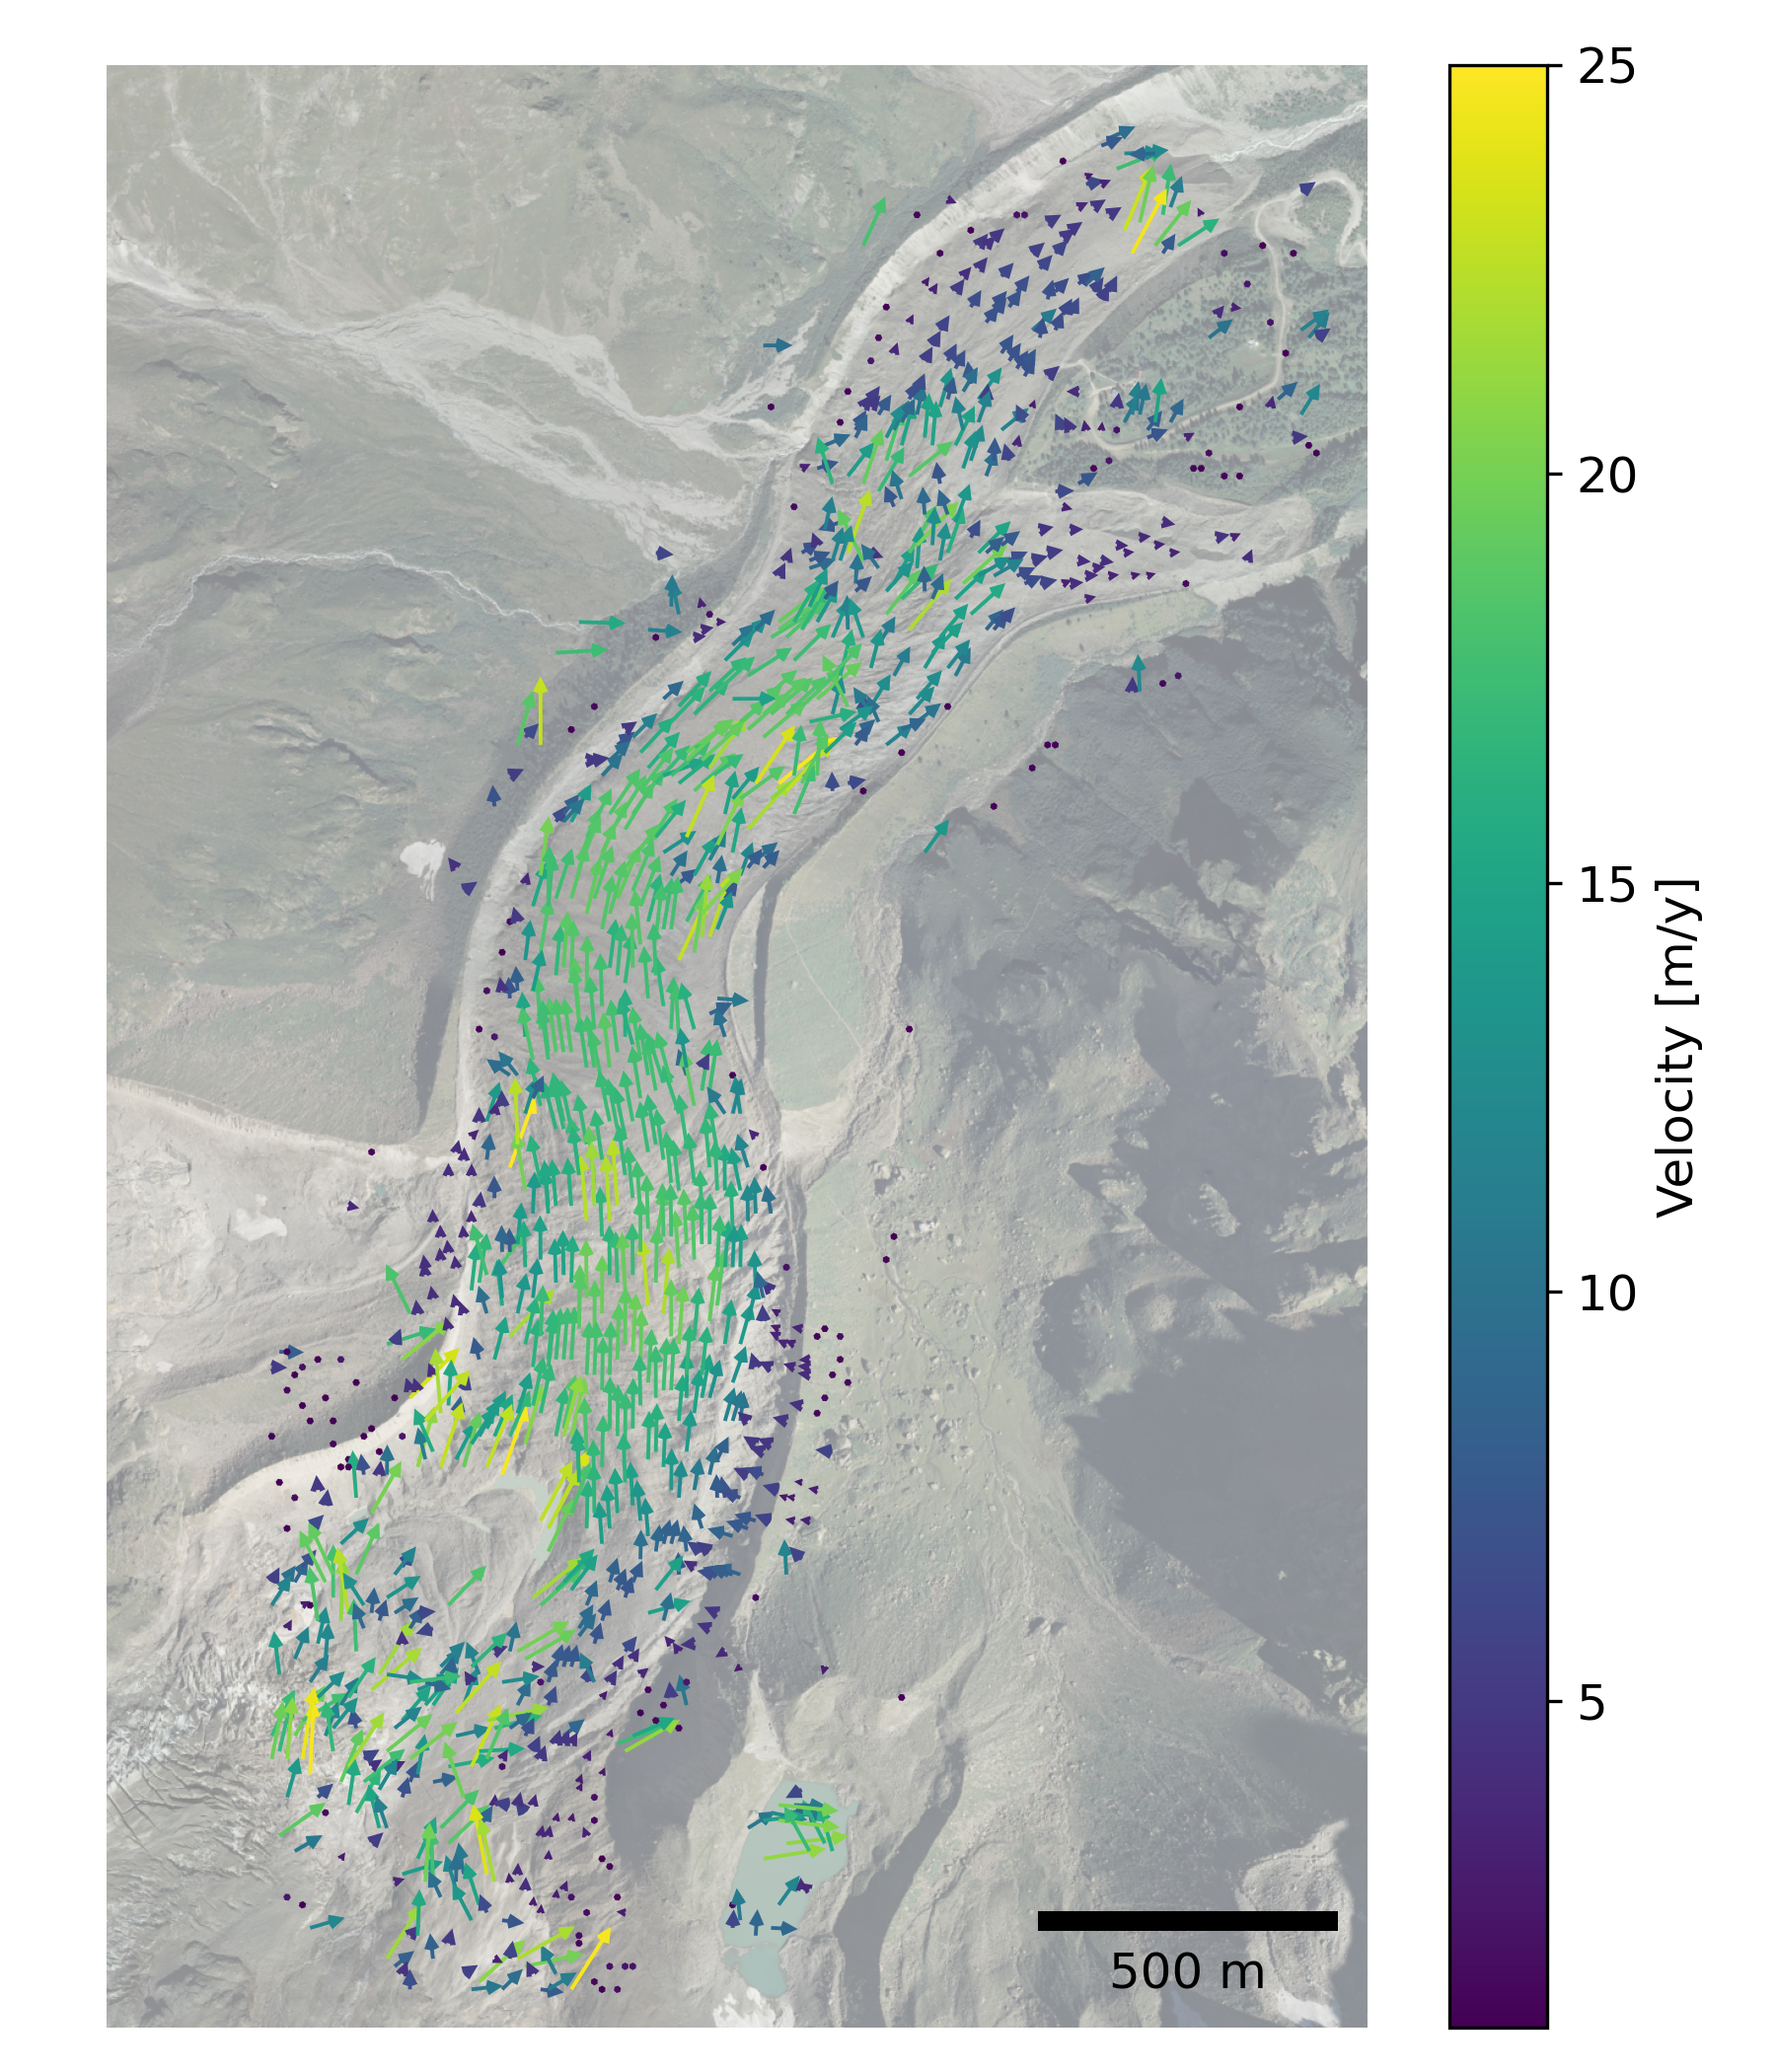
\includegraphics[width=0.44\textwidth]{velocity_DIC_2016-2017}
    } \\
    \subcaptionbox{2017-2018\label{fig:3:dic_vel:2017}}{
        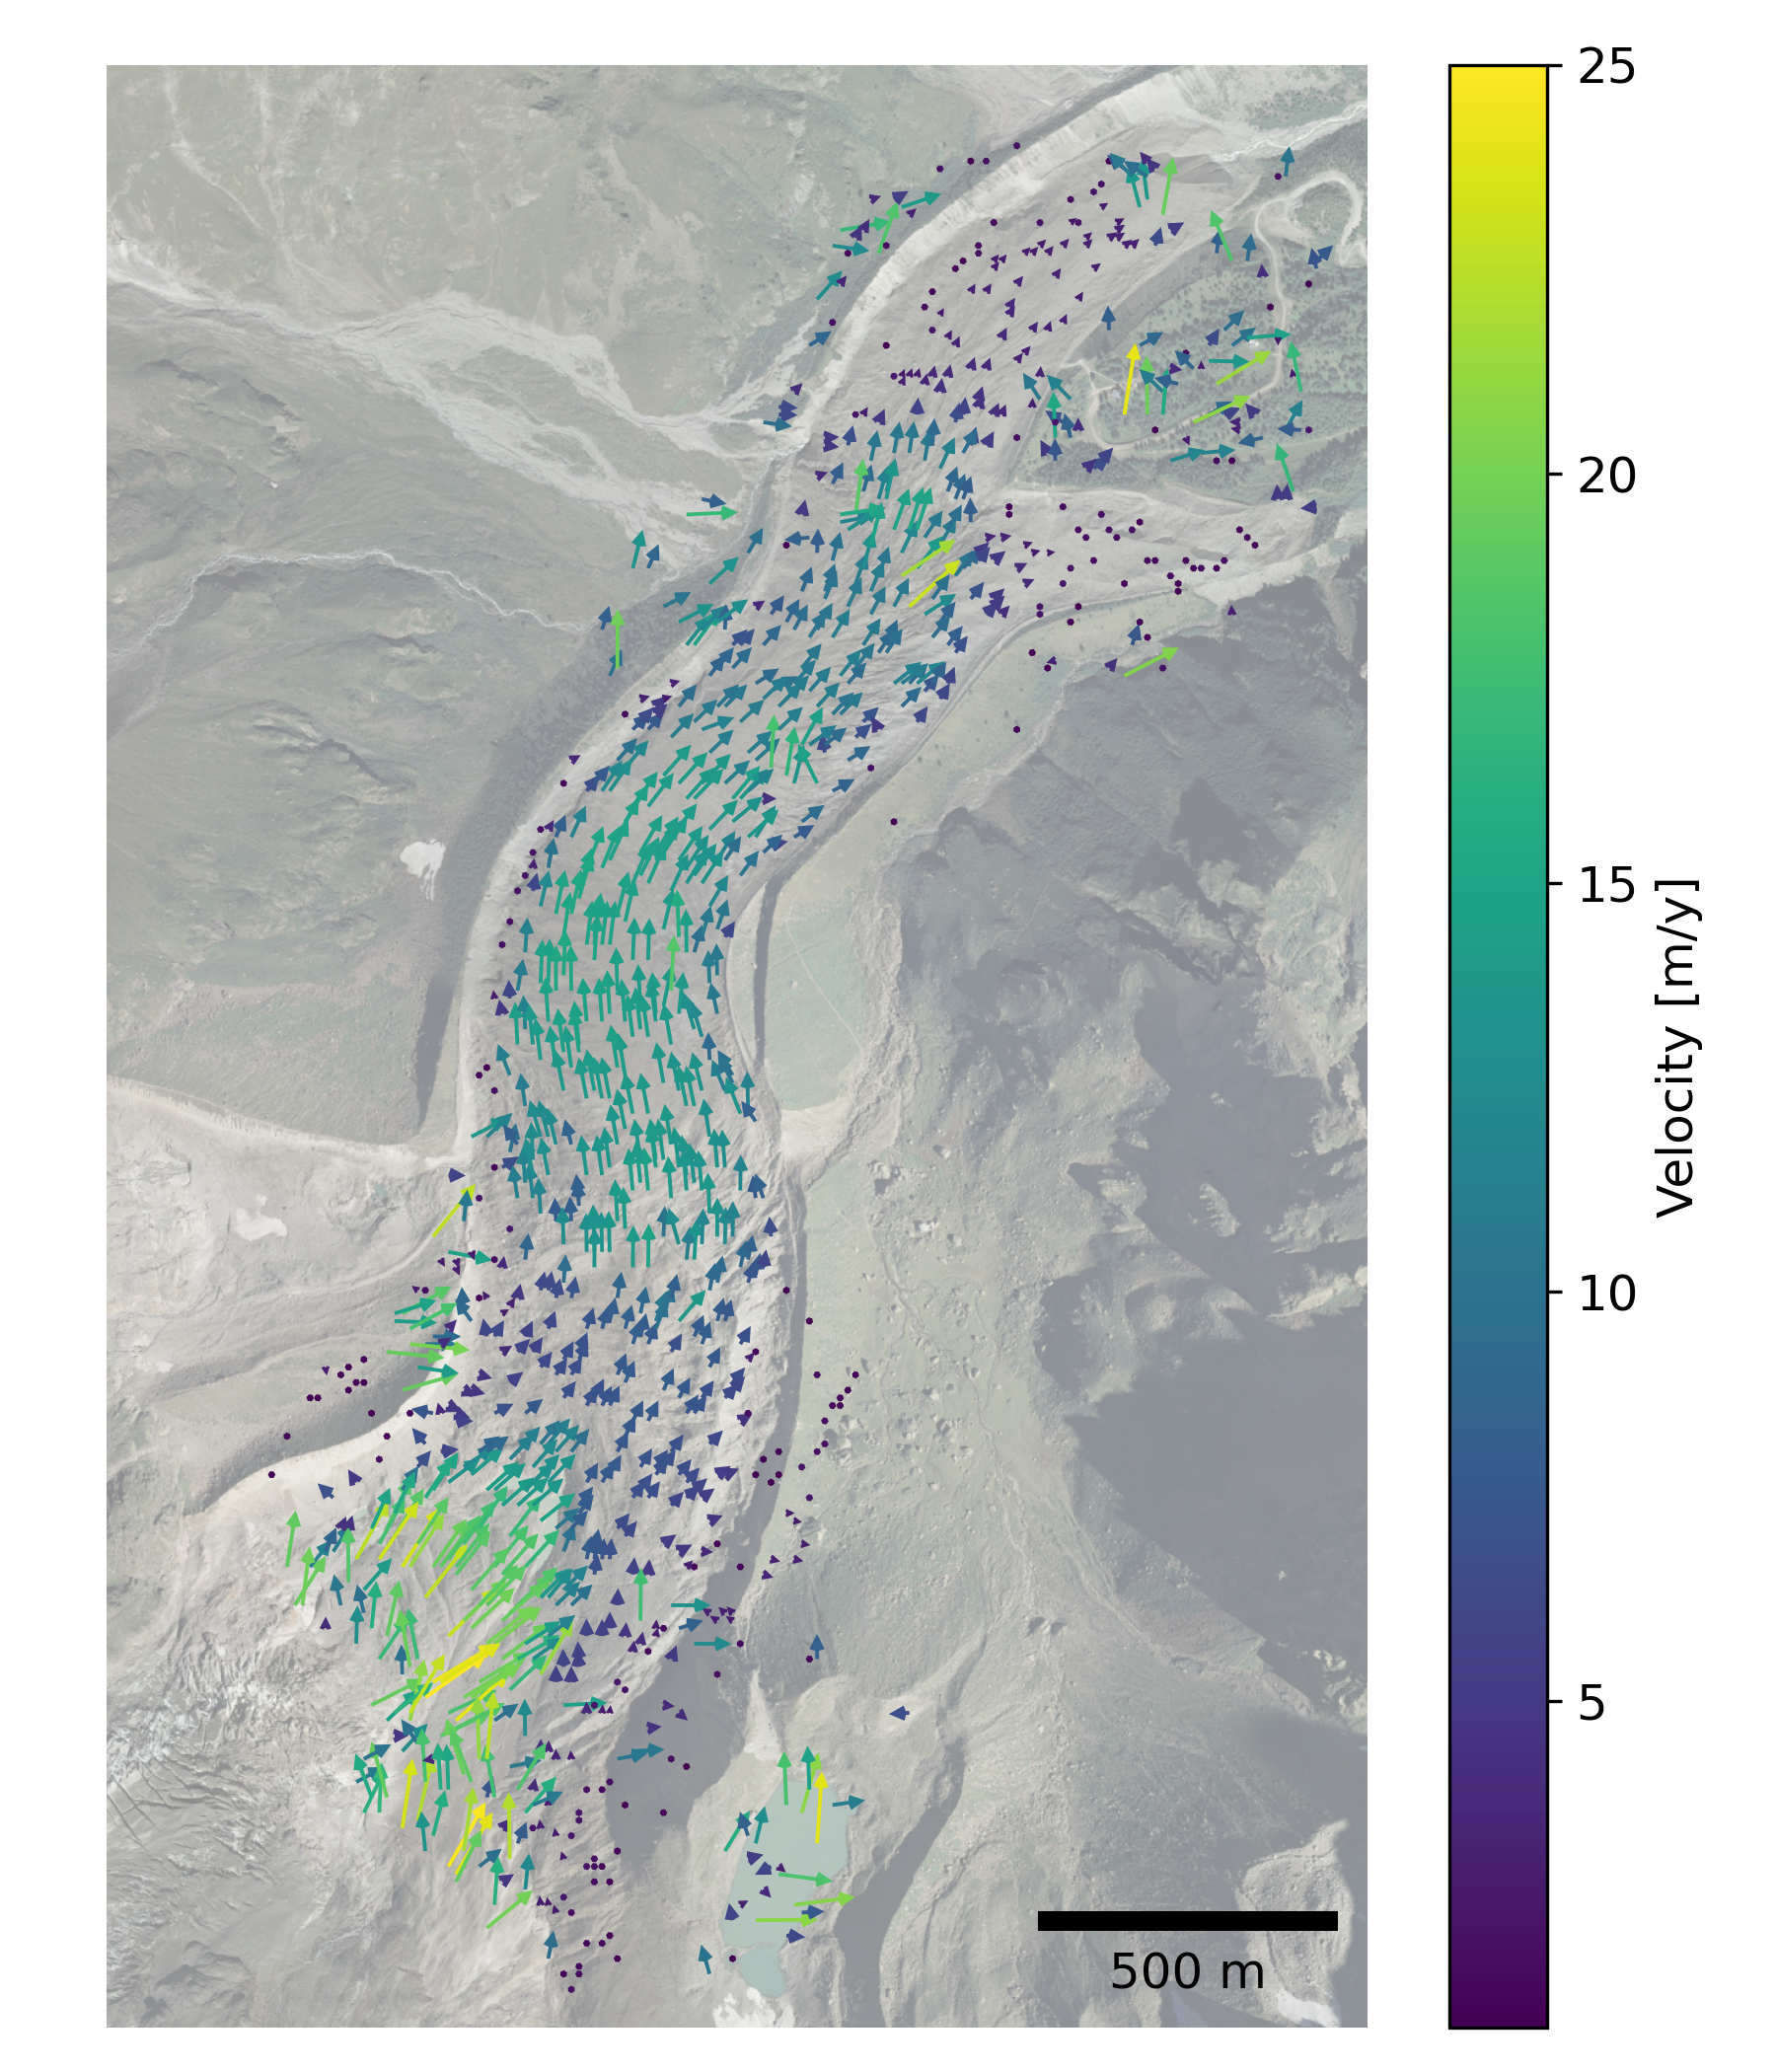
\includegraphics[width=0.44\textwidth]{velocity_DIC_2017-2018}
    } 
    \subcaptionbox{2018-2019\label{fig:3:dic_vel:2018}}{
        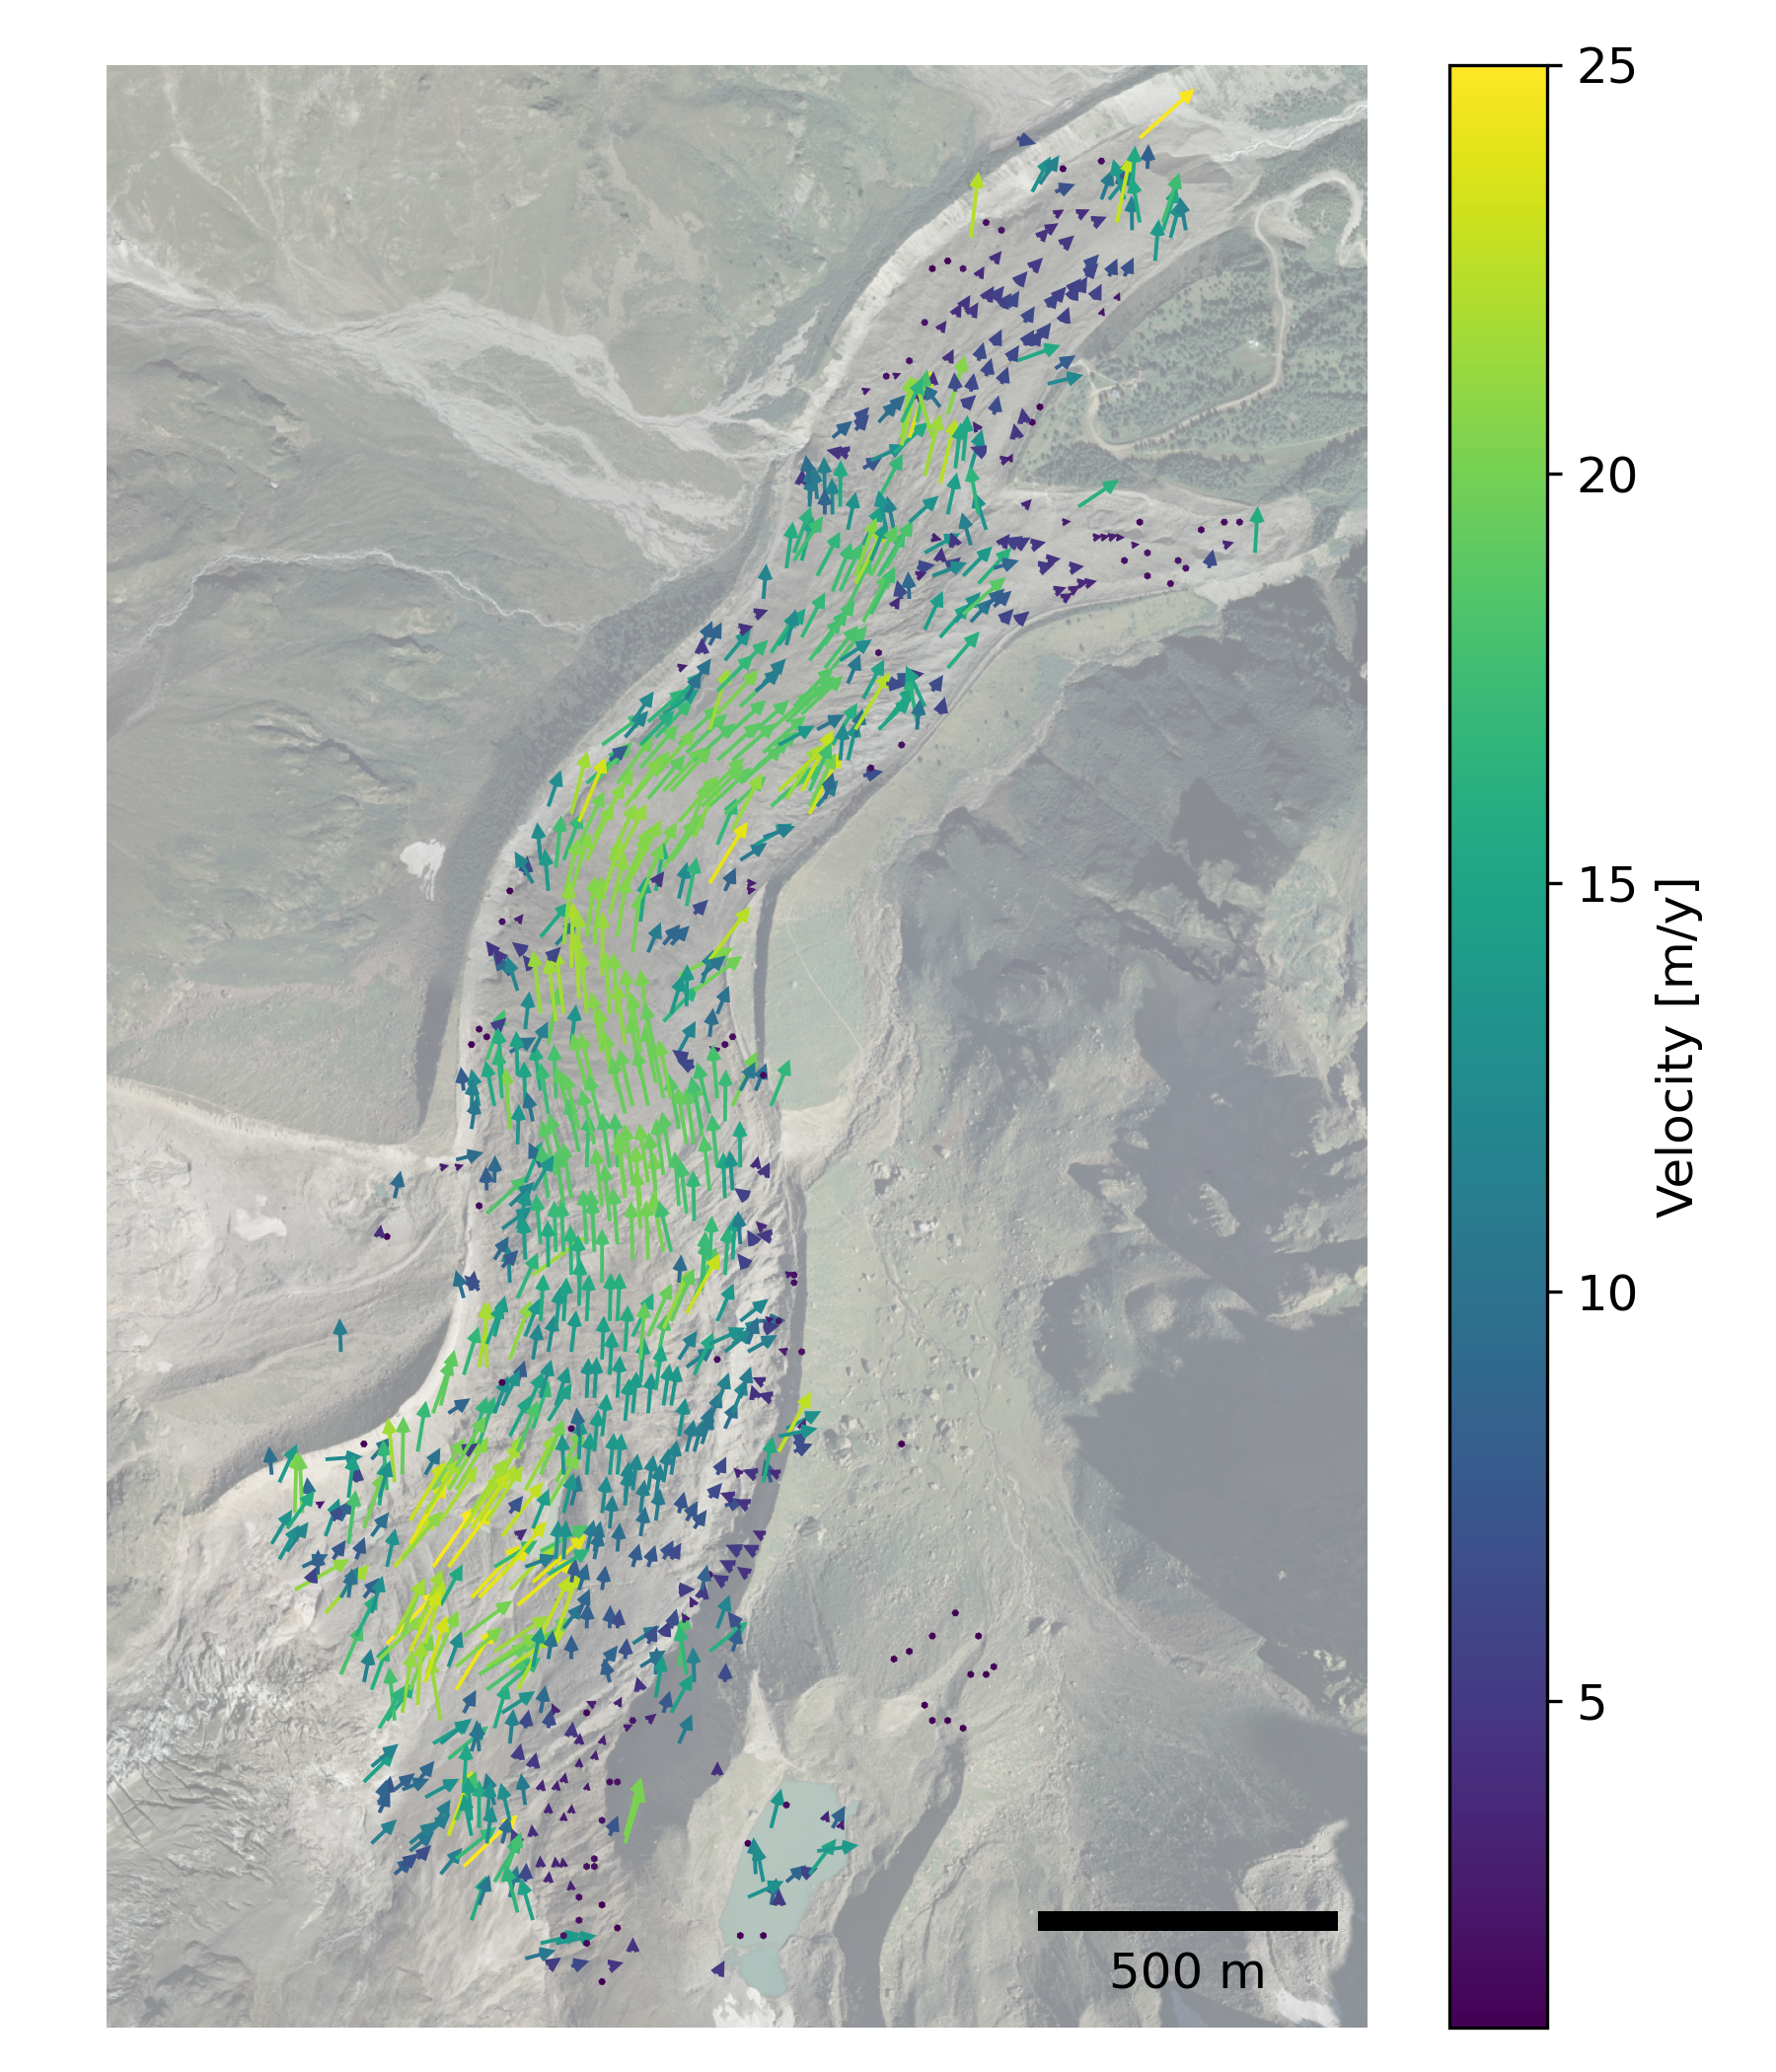
\includegraphics[width=0.44\textwidth]{velocity_DIC_2018-2019}
    }
    \caption{Surface velocity fields derived by DIC on pair of consecutive DSM between 2015 and 2018 and 
    orthophotos between 2019 and 2023. (\textbf{a}) 2015-2016, (\textbf{b}) 2016-2017, (\textbf{c}) 2017-2018, (\textbf{d}) 2018-2019.
    All the surface velocity fields are overlapped to the 2009 orthophoto \citep{Degaetani2021} as reference. Refer to the Appendix \ref{app:sfv} for better visualization of the orthophotos  (continue on the next page).}
    \label{fig:3:dic_vel}
\end{figure}

\begin{figure}[!p]\ContinuedFloat
    \centering
    \subcaptionbox{2019-2020\label{fig:3:dic_vel:2019}}{
        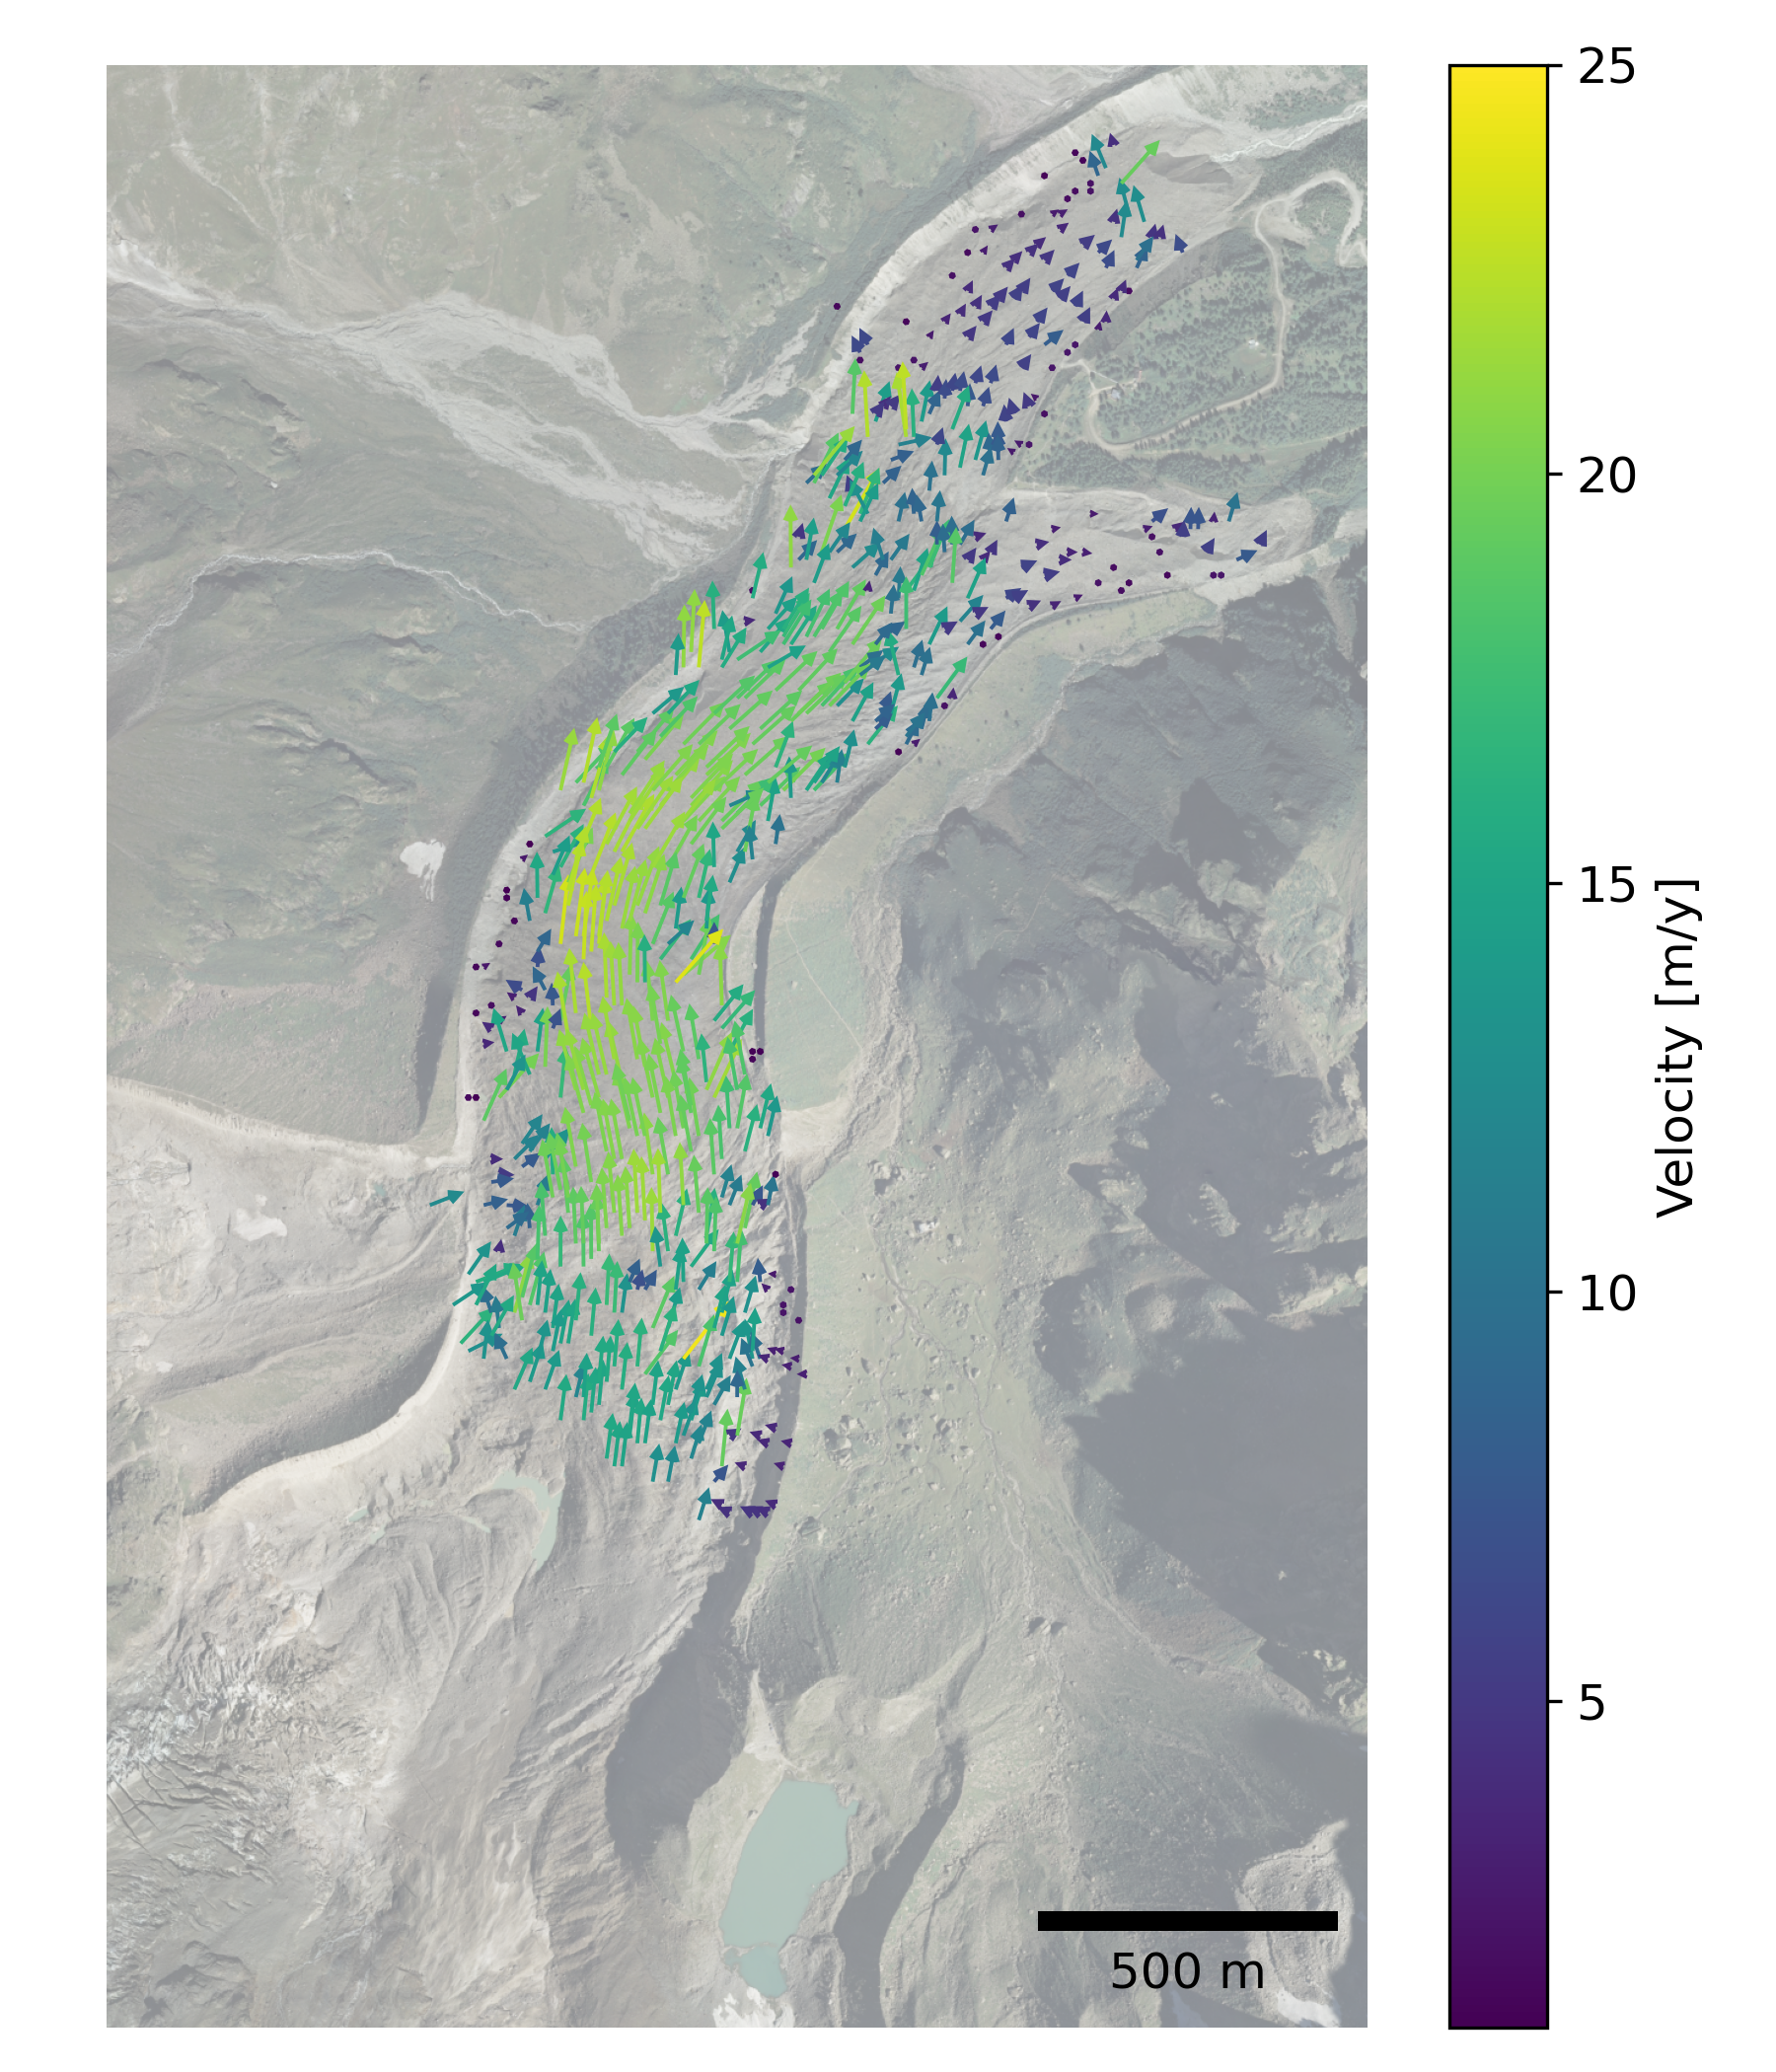
\includegraphics[width=0.44\textwidth]{velocity_DIC_2019-2020}
    }
    \subcaptionbox{2020-2021\label{fig:3:dic_vel:2020}}{
        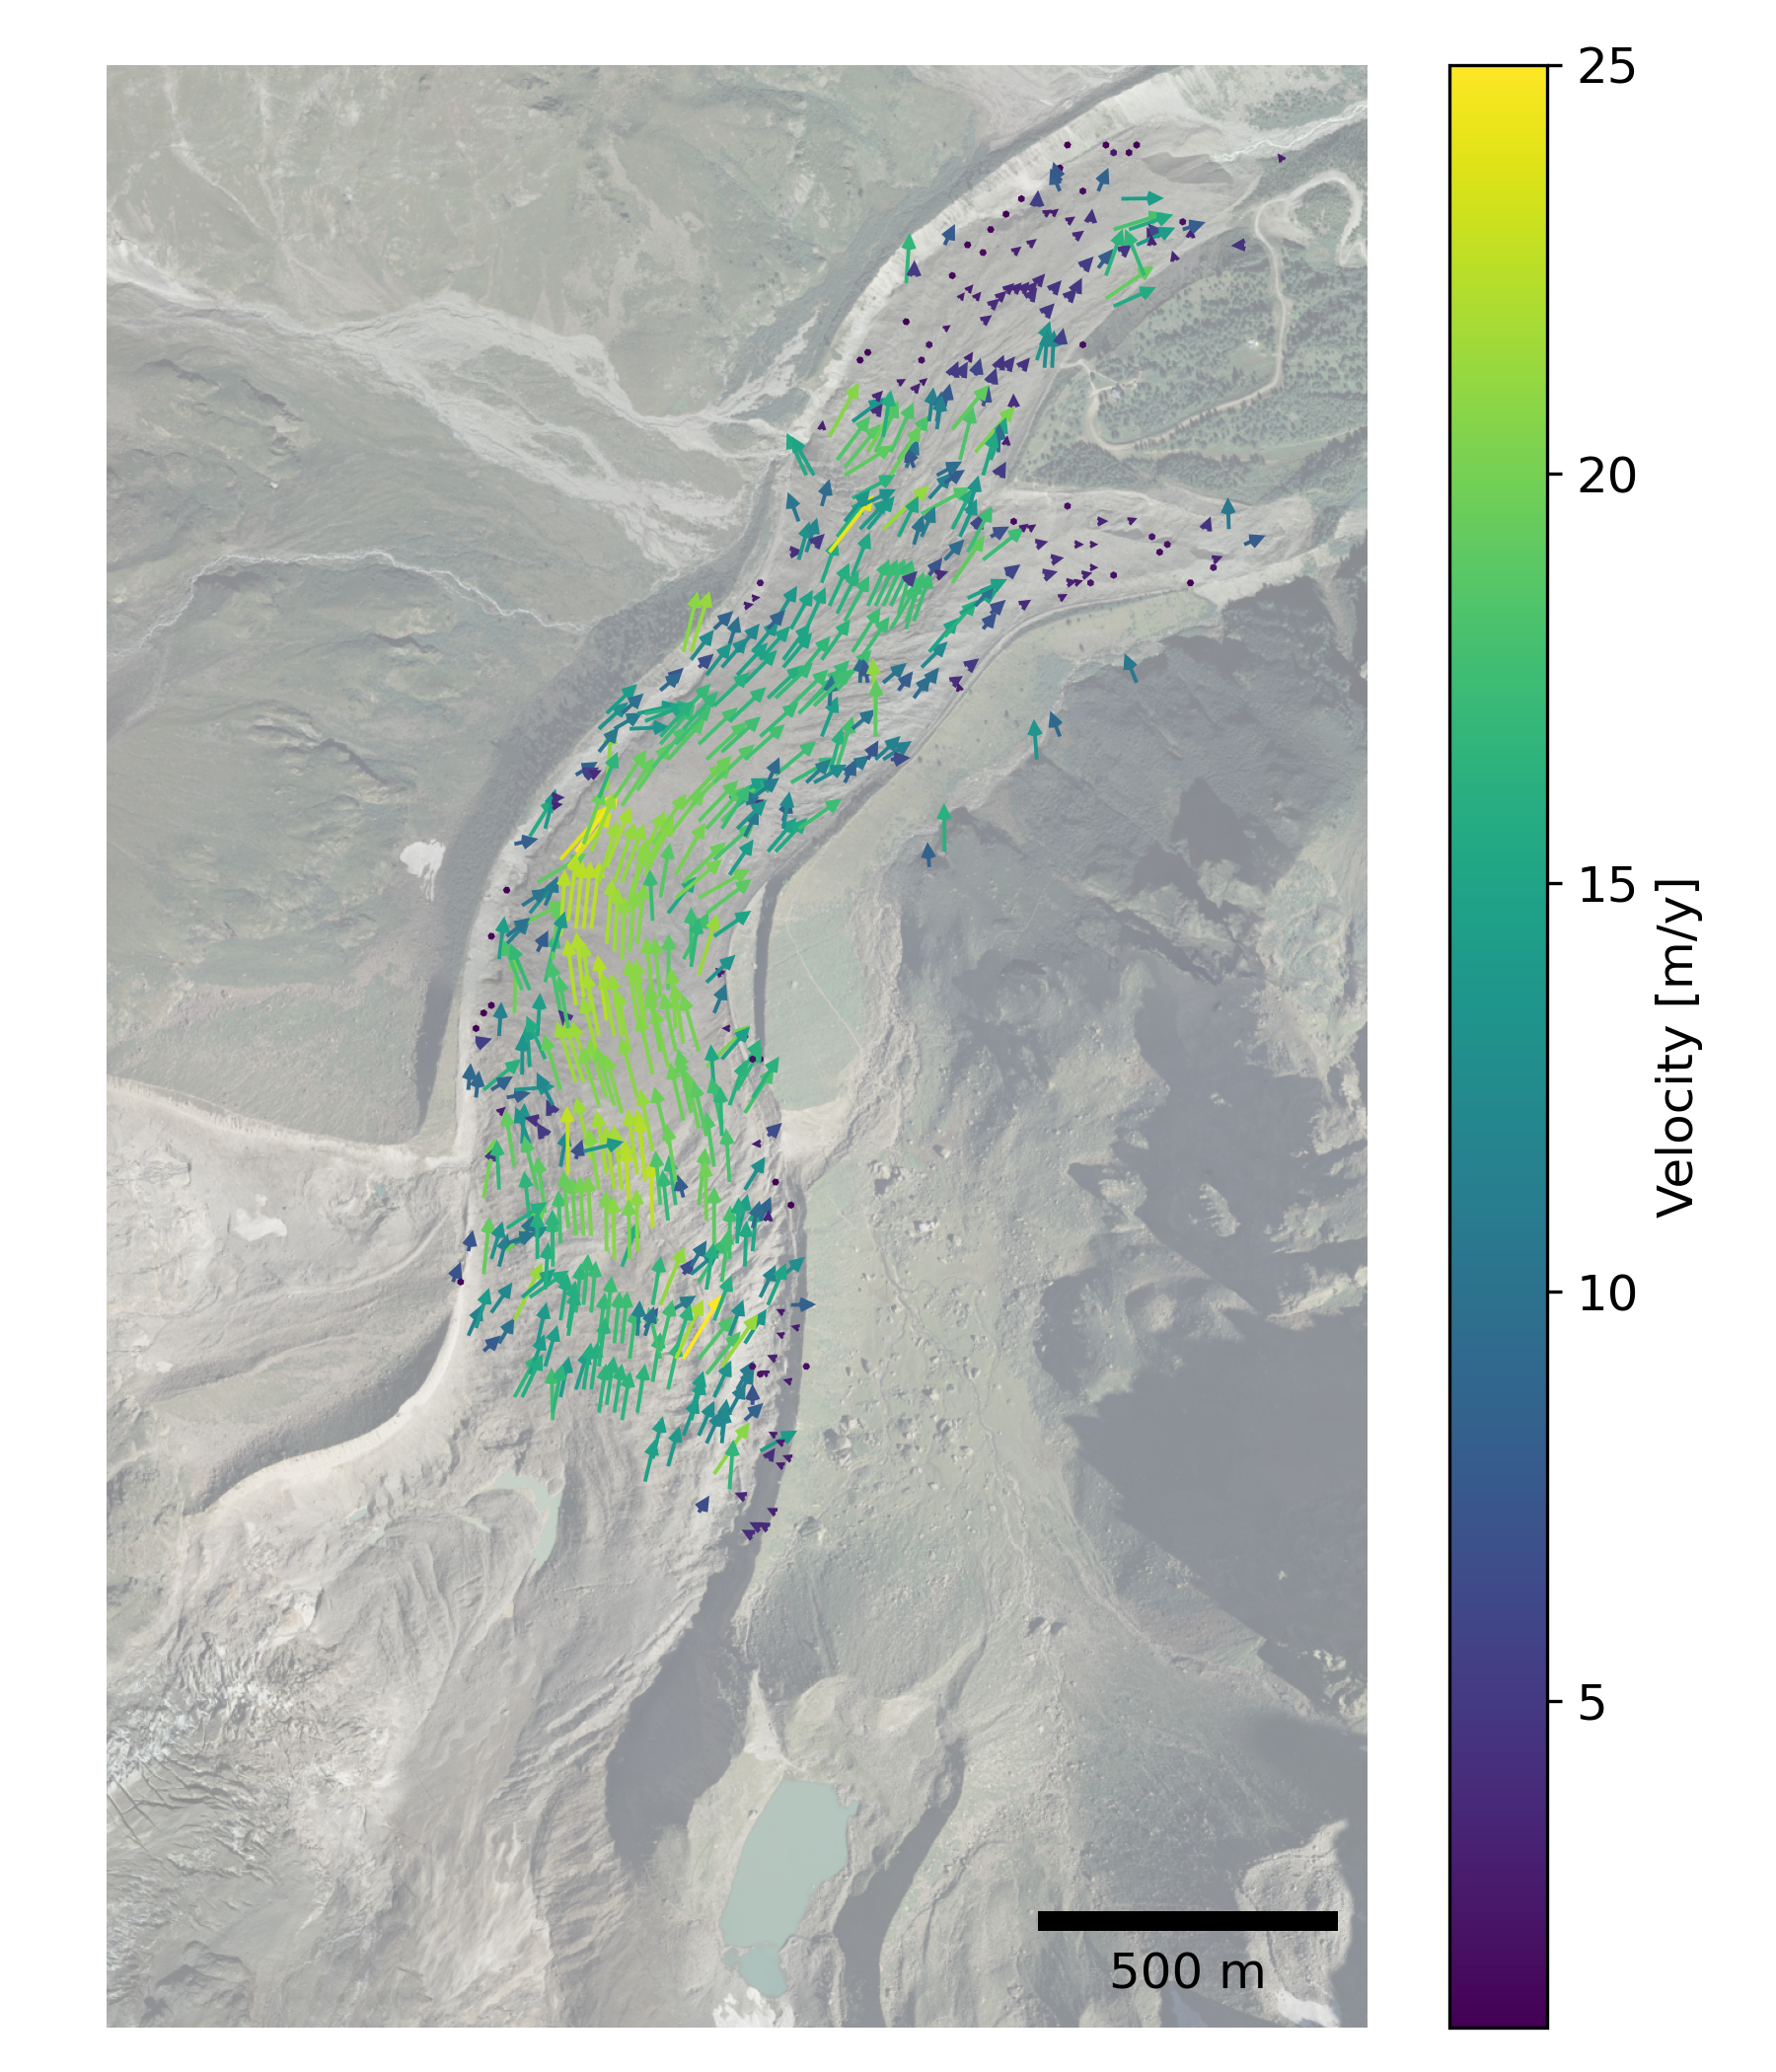
\includegraphics[width=0.44\textwidth]{velocity_DIC_2020-2021}
    }    
    \subcaptionbox{2021-2022\label{fig:3:dic_vel:2021}}{
        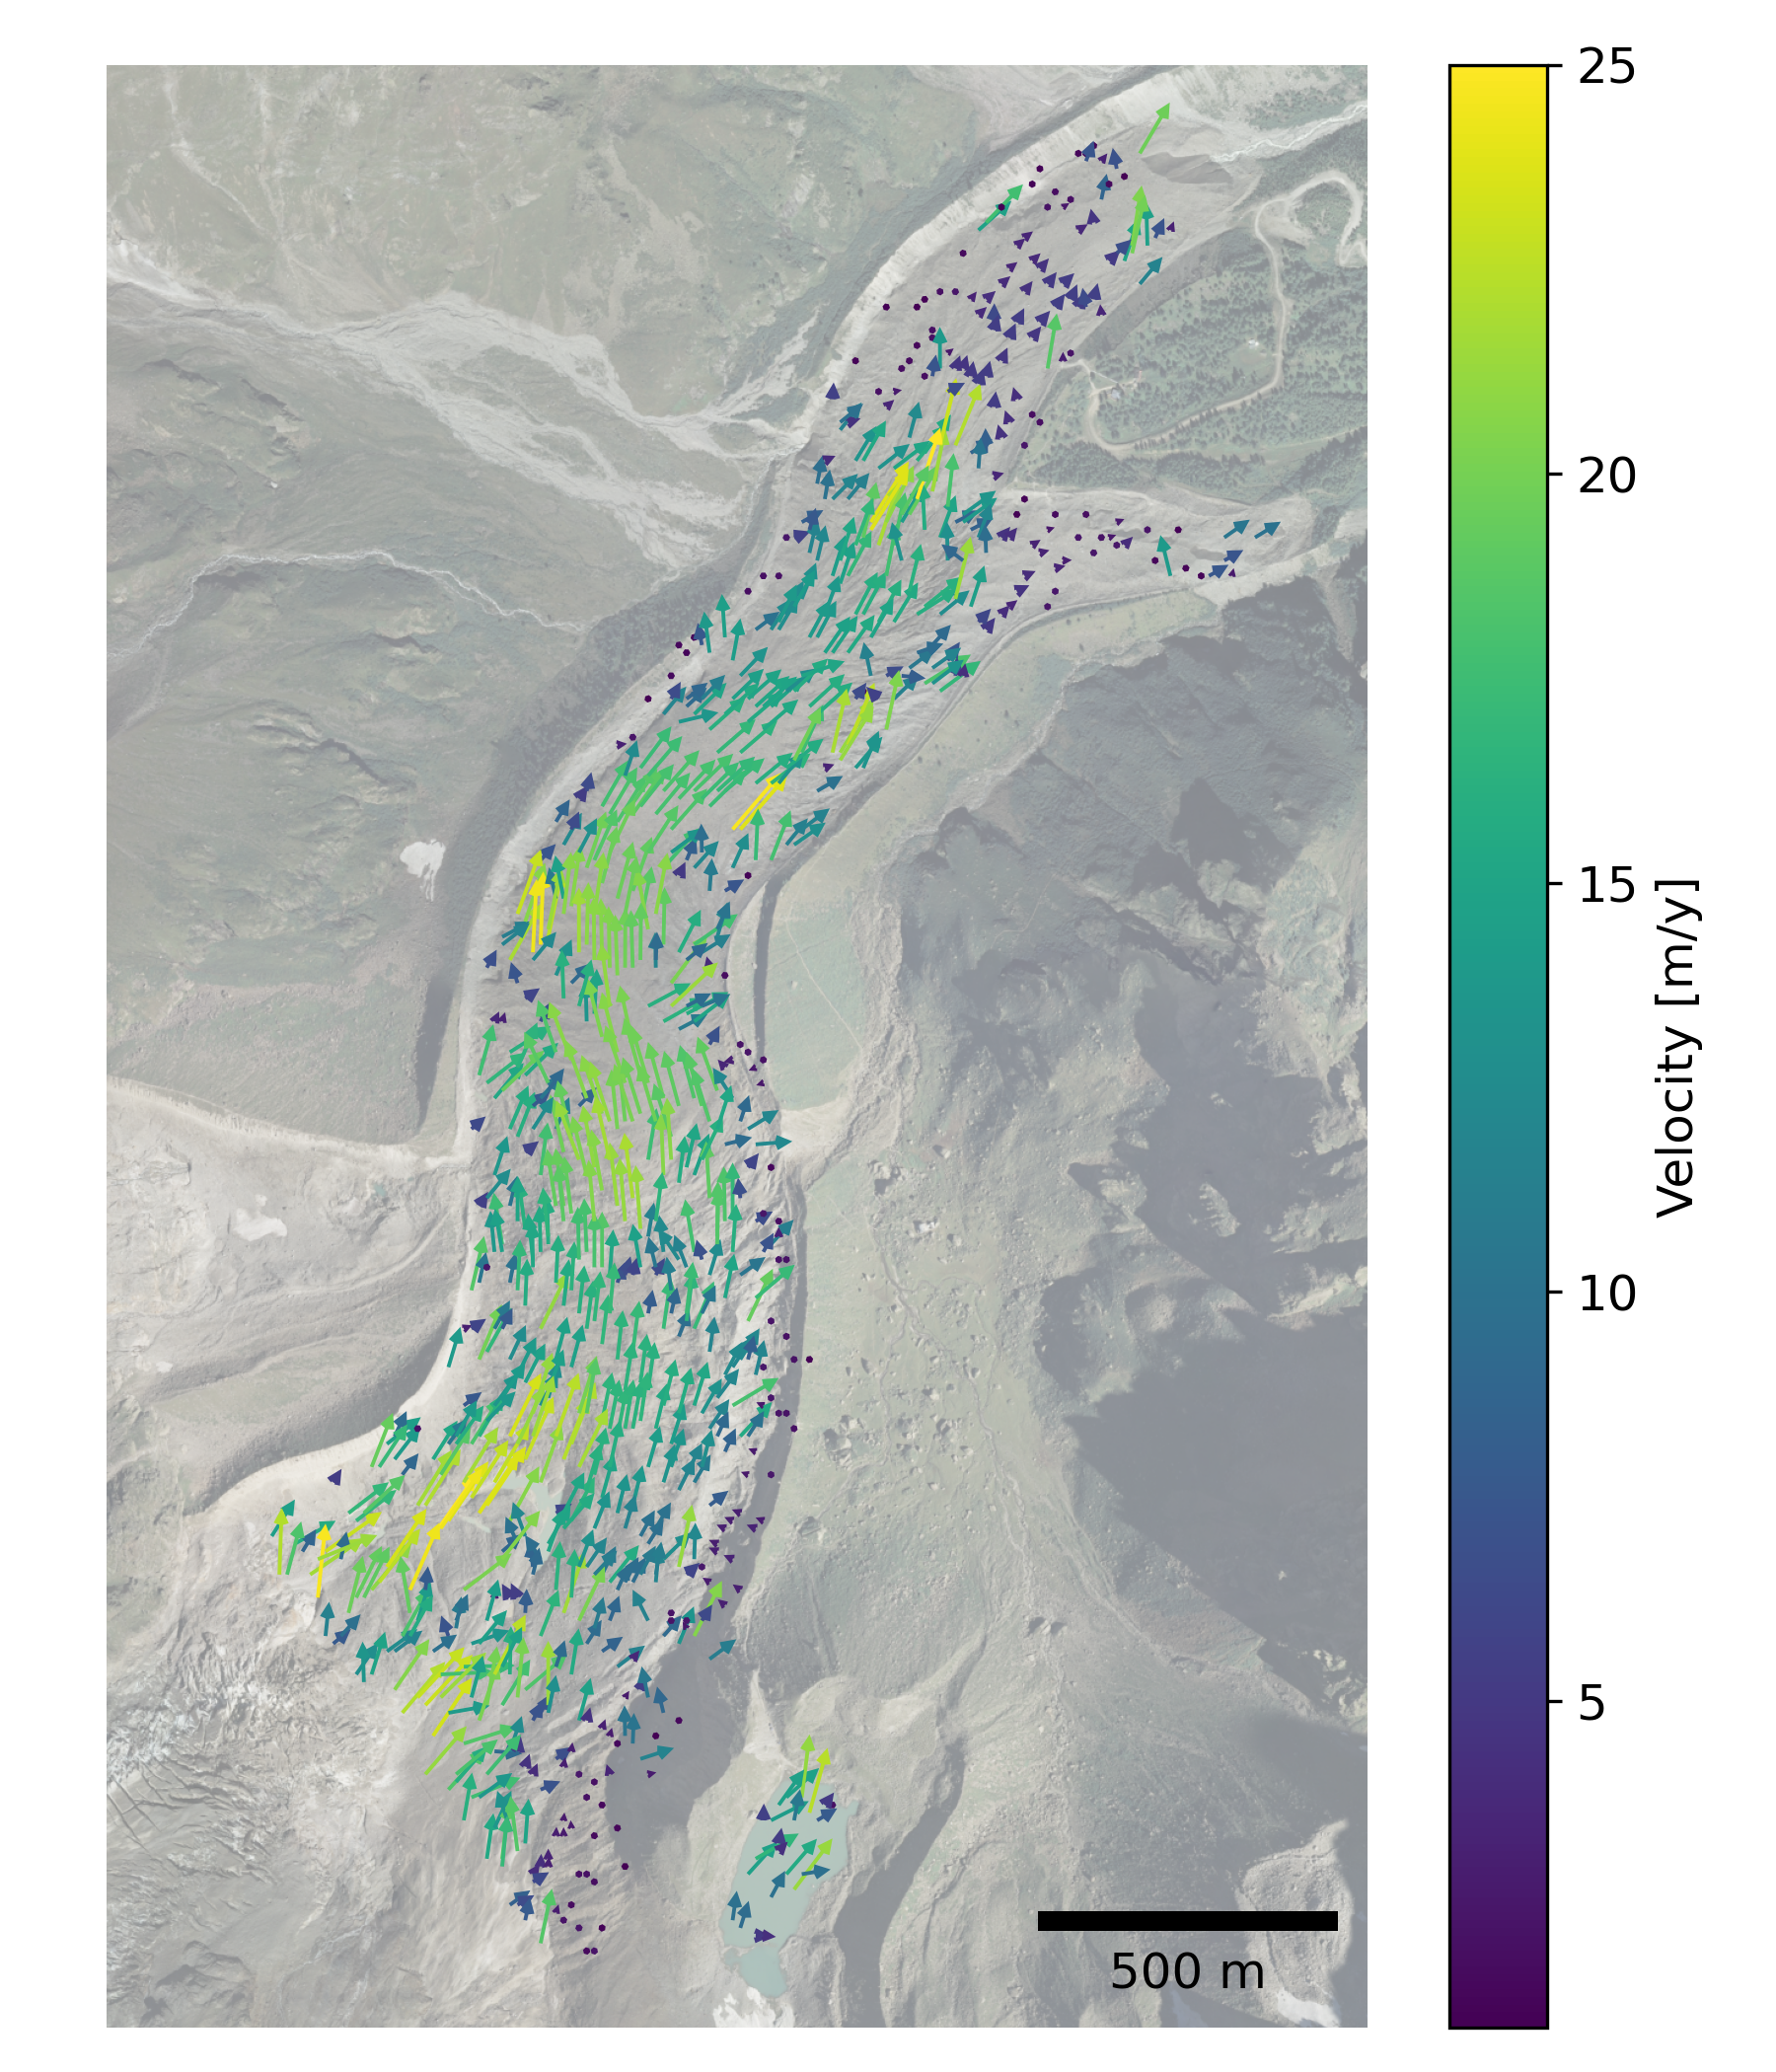
\includegraphics[width=0.44\textwidth]{velocity_DIC_2021-2022}
    } 
    \subcaptionbox{2022-2023\label{fig:3:dic_vel:2022}}{
        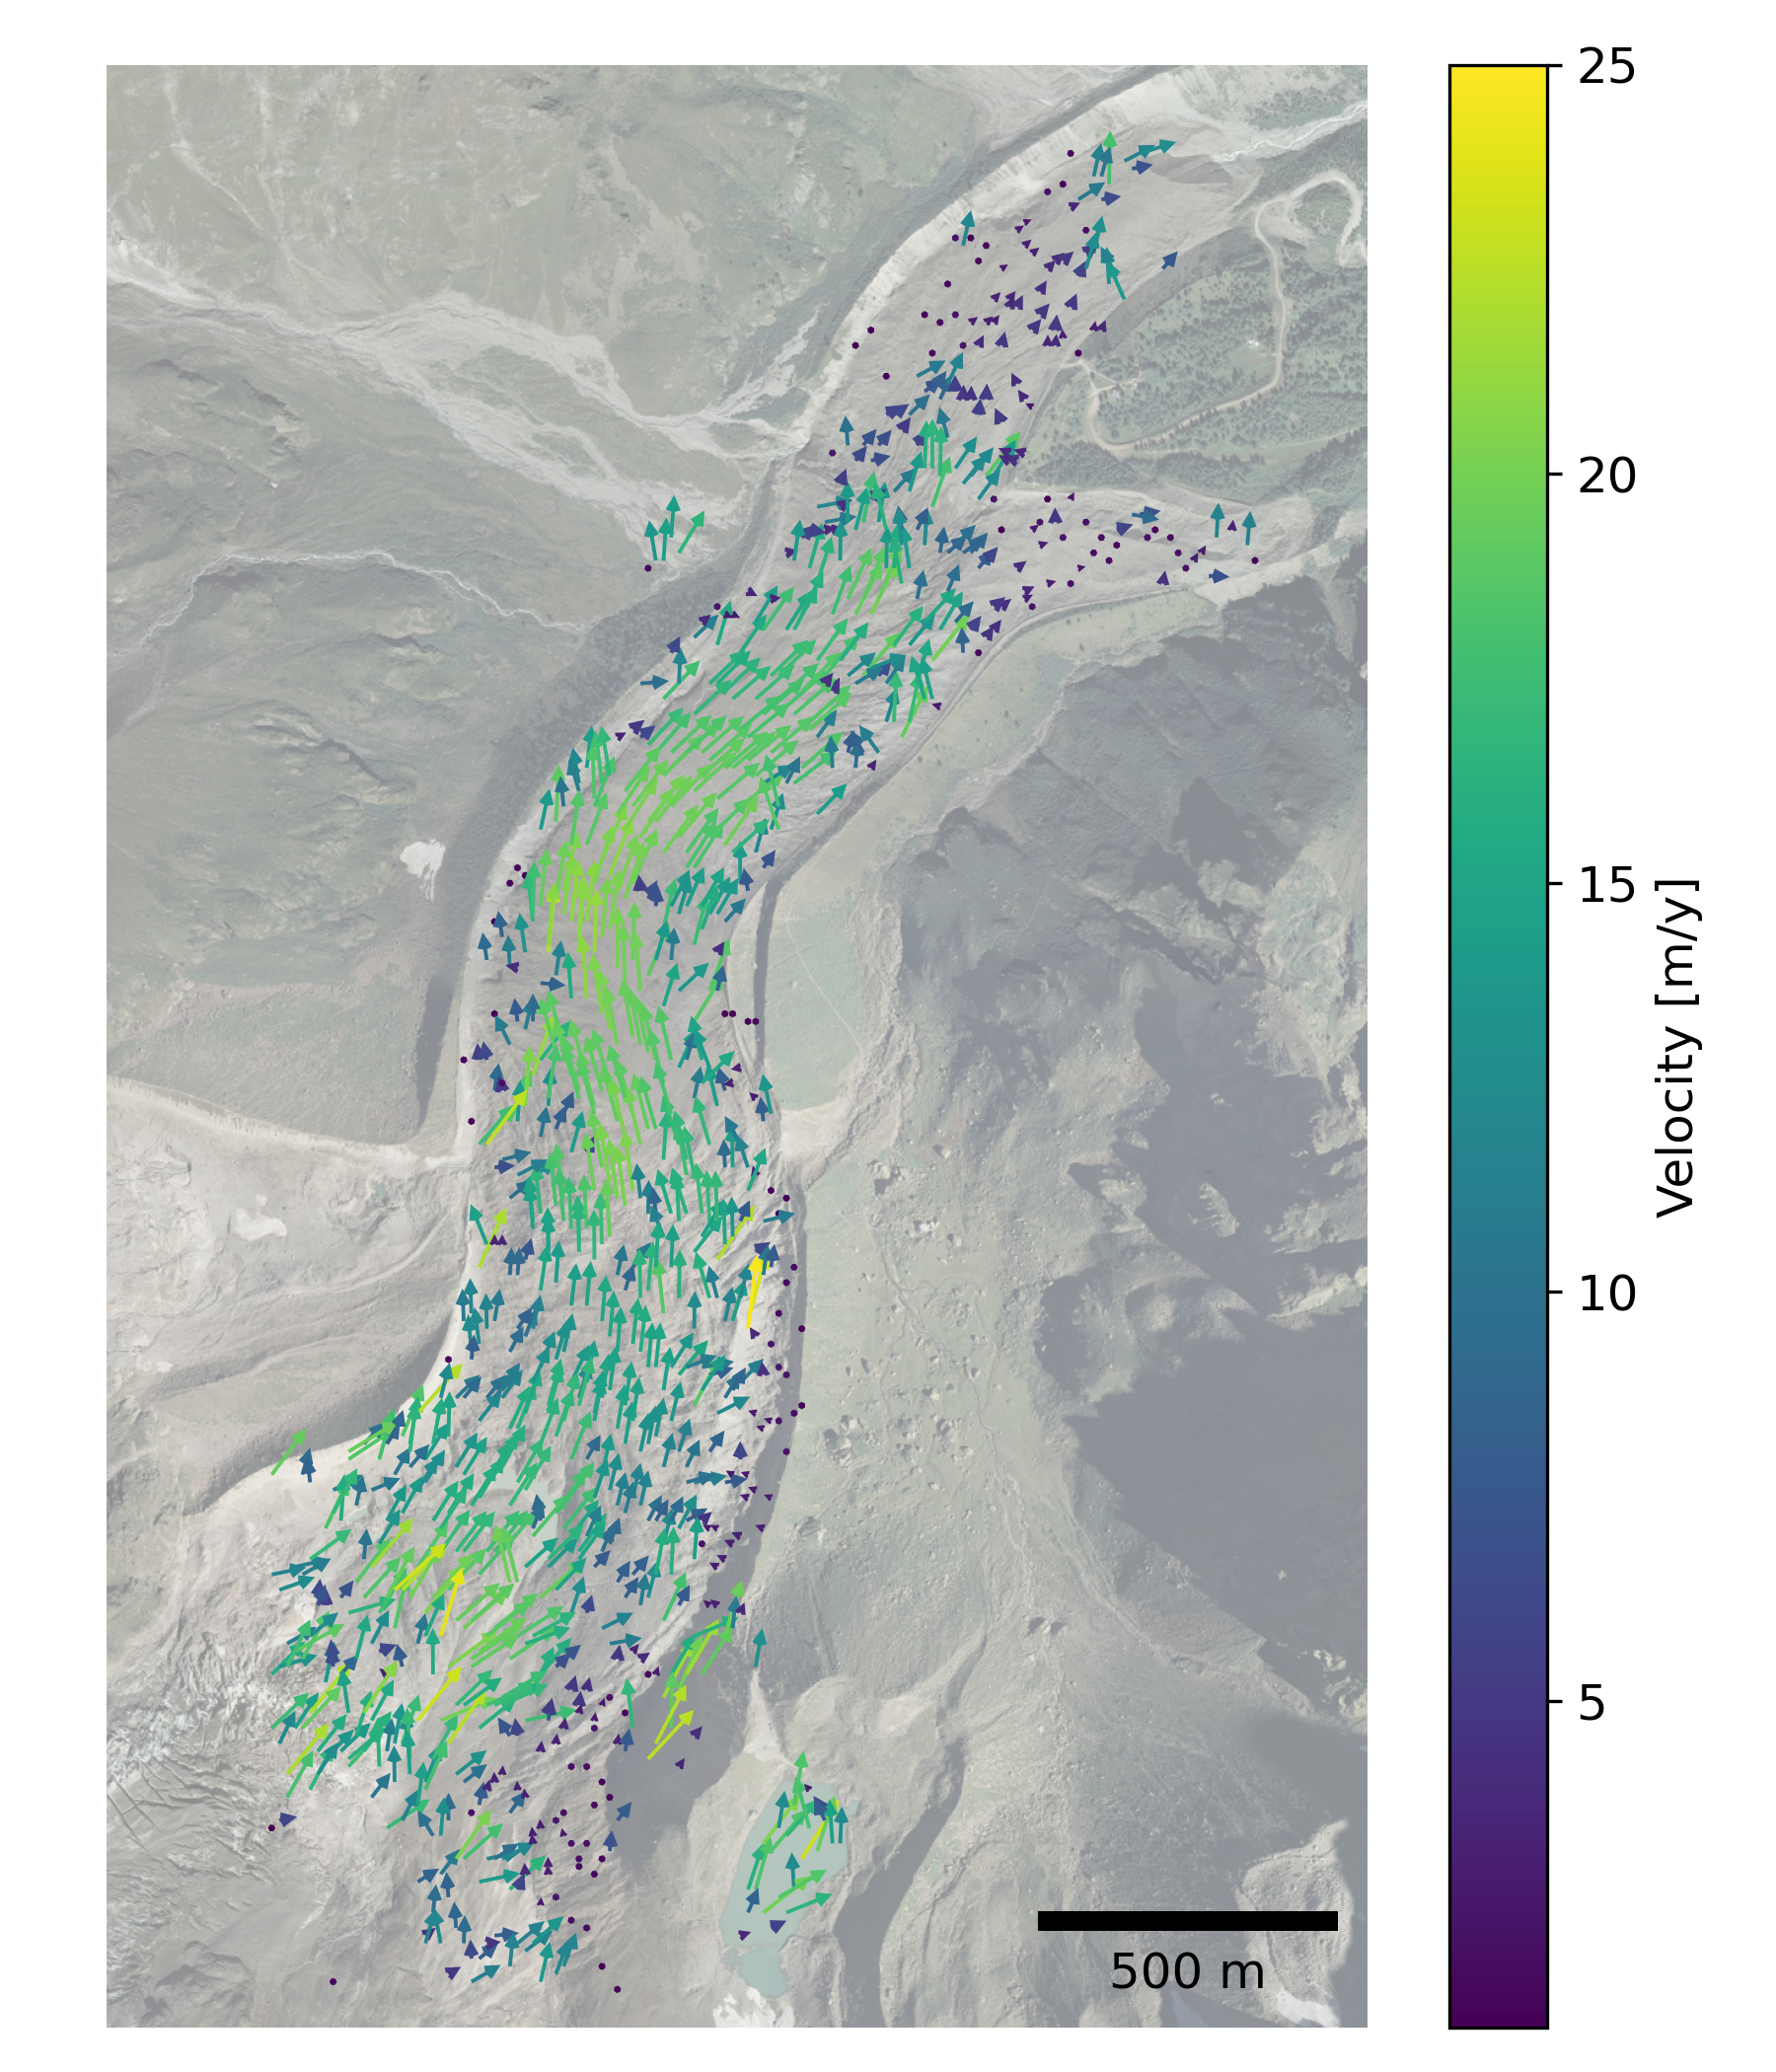
\includegraphics[width=0.44\textwidth]{velocity_DIC_2022-2023}
    }
    \caption{Surface velocity fields derived by DIC on pair of consecutive DSM between 2015 and 2018 and 
    orthophotos between 2019 and 2023. (\textbf{e}) 2019-2020, (\textbf{f}) 2020-2021, (\textbf{g}) 2021-2022, (\textbf{h}) 2022-2023.
    All the surface velocity fields are overlapped to the 2009 orthophoto \citep{Degaetani2021} as reference. Refer to the Appendix \ref{app:sfv} for better visualization of the orthophotos (cont.).}
\end{figure}

The surface velocity fields, derived from both orthophotos and DSMs, are presented in \figref{fig:3:dic_vel}. 
We employed DIC on DSM pairs for the 2015-2018 period and orthophotos for 2019-2023 (see \secref{sec:3:method_velocity} for methodological details). 
The results agree with those obtained from GNSS measurements, highlighting the same velocity distribution along the glacier.
Additionally, DIC results allow us to appreciate the velocity distribution along the glacier transects. 
As expected, the highest velocities are found along the centerline, gradually decreasing towards the moraines due to increased friction between the glacier and the underlying bedrock and the glacier's thinner ice at the edges.

The 2017-2018 velocity field (\figref{fig:3:dic_vel:2017}) exhibits significantly lower velocities than other years. 
This discrepancy is attributed to the shift in survey dates from autumn to summer (see \secref{sec:3:problems}). 
The DSMs used for this period (acquired in October/November 2017 and July 2018) do not encompass the peak glacier ablation and velocity season during summer. 
In contrast, all other surveys were consistently carried out either in autumn (pre-2017) or summer (2018 onwards), ensuring comparability.  
Additionally, the surface fields from 2019-2021 lack results in the glacier's upper portion due to the limitations in the 2020 SfM model \secref{sec:3:problems}).

\begin{figure}
    \centering
    \subcaptionbox{\label{fig:3:velocity_time_series:ts}}{
        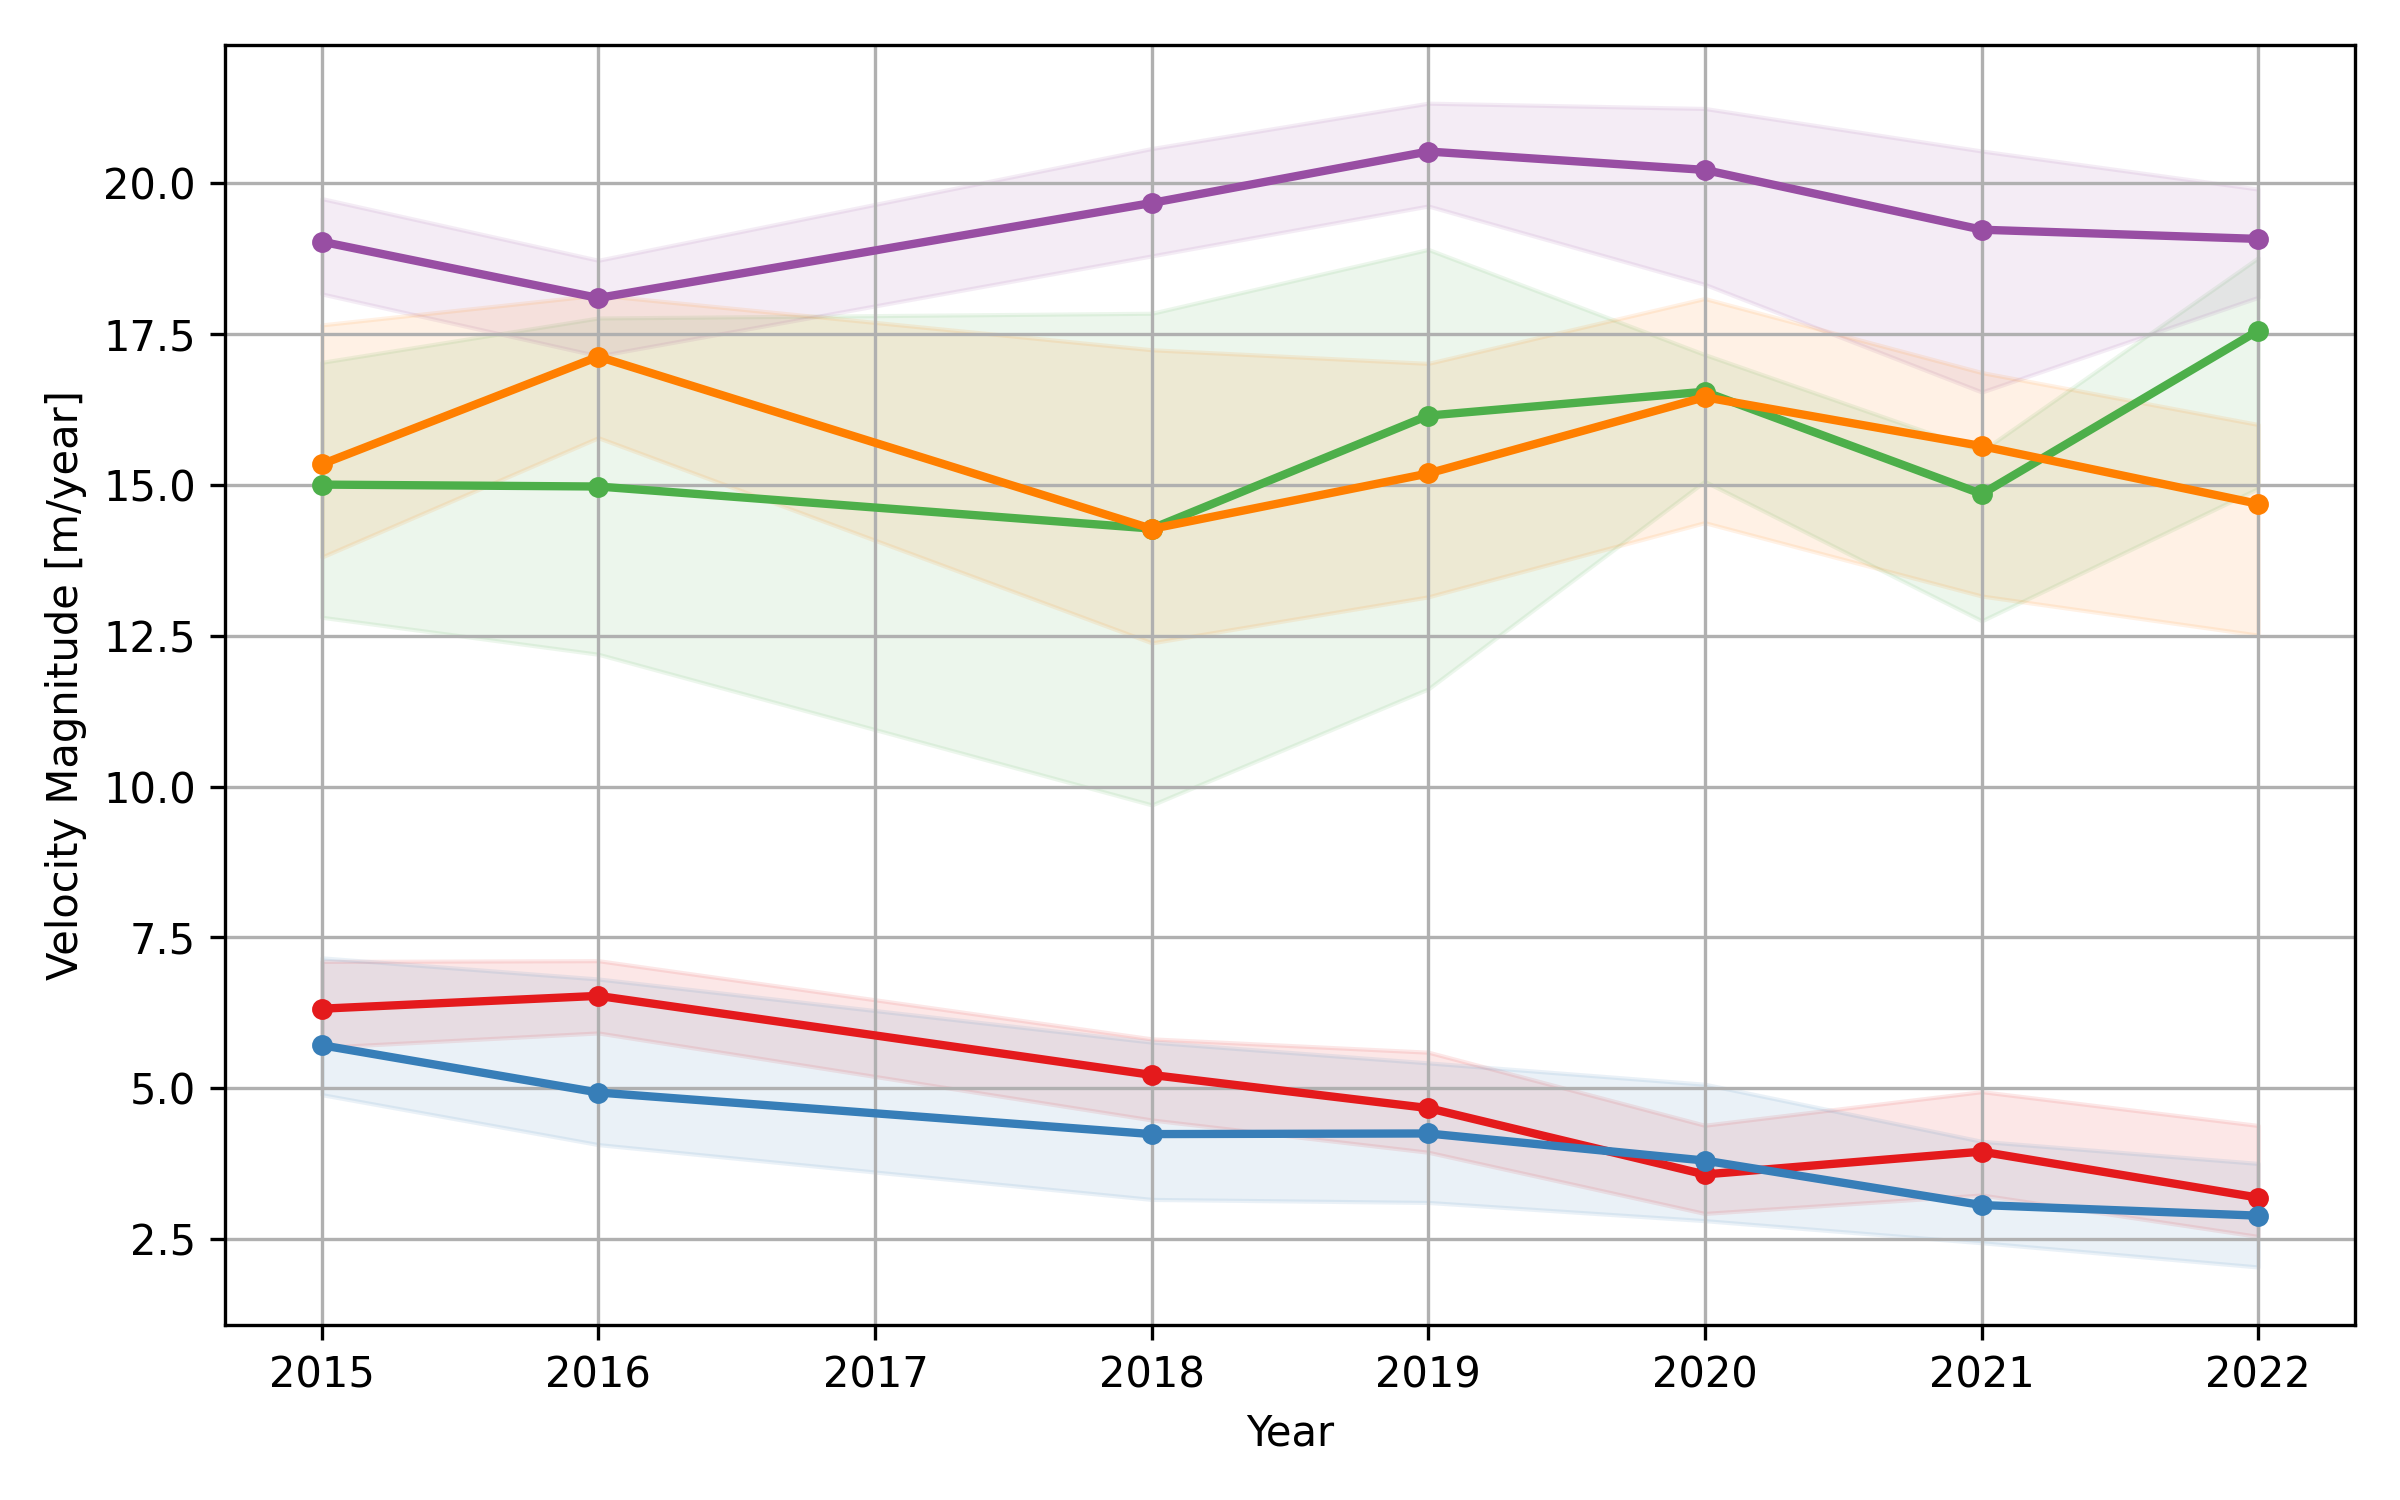
\includegraphics[height=6.3cm]{velocity_time_series.png}
    } \hfill
    \subcaptionbox{\label{fig:3:velocity_time_series:map}}{
        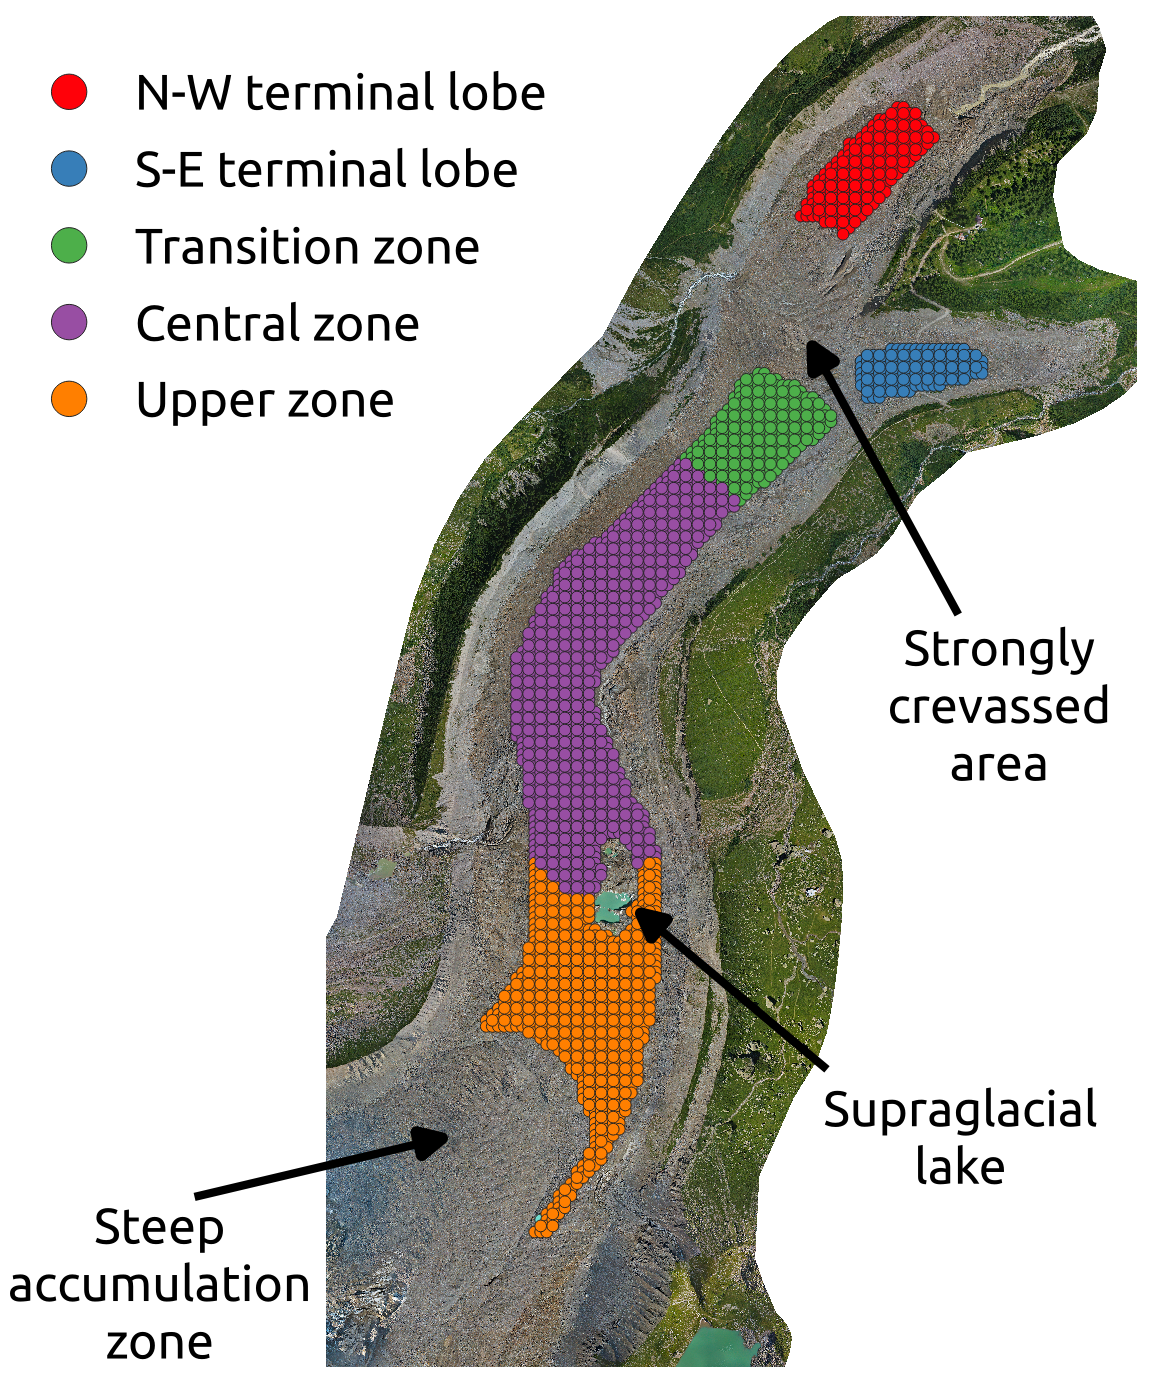
\includegraphics[height=5.5cm]{velocity_time_series_clusters.png}
    }
    \caption{(\textbf{a})Time series of median annual velocities for each cluster derived from DIC. The solid lines represent the median velocity, while the light-colored bands indicate the interquartile range, visualizing velocity variability within each cluster. Cluster colors correspond to the spatial mapping in (b). Marker positions correspond to the year of the master image used in DIC processing (i.e., the first image of each pair). The velocity value obtained from 2017-2018 was excluded from the time series; (\textbf{b}) Location of clusters with homogeneous movement patterns.}
    \label{fig:3:velocity_time_series}
\end{figure}

The grid nodes used for DIC computations were subdivided into groups with similar kinematics according to the clusters identified by the GNSS measurements (\figref{fig:3:velocity_time_series:map}). 
These groups included the slow-moving terminal lobes, a transition zone between the lobes and the glacier's main transfer zone, the fast central zone, and the upper zone.  
Nodes near glacier moraines (where friction reduces surface velocity) and nodes in areas prone to decorrelation between years were excluded, e.g., the heavily crevassed region near the terminal lobe junction, areas with recurrent supraglacial lake formation, or areas where subglacial streams create cavities and pronounced ice cliffs.
The remaining nodes were used to calculate the median annual velocity of each cluster. 
\figref{fig:3:velocity_time_series:ts} visualizes these time series of the median velocity, along with the Interquartile Range (IQR, i.e., the difference between the 0.75 and 0.25 percentiles of the empirical distribution) of the velocity vectors of each cluster for each year.
Velocity values obtained by DIC between 2017 and 2018 were excluded from the analysis due to the velocity underestimation related to the change in the survey date. 

A strong velocity contrast exists between the glacier's slower terminal lobes and its faster-flowing central zone.  
The gradual velocity decline observed in the two terminal lobes is particularly interesting. 
This trend is probably related to the extreme ice thinning documented in this region in recent years, as a reduced ice thickness leads to slower flow velocities~\citep{Cuffey2010_physics_glaciers,jiskoot2011dynamics_glacier}.
A generalized glacier slowdown linked to a negative mass balance trend was also sensed in various regions around the globe between 1953 and 2009 \cite{Heid2012a} and in  High Mountain Asia between 2000 and 2017 \cite{Dehecq2019}.
In fact, at the terminal lobes, where the ice thickness is smaller, the ice thinning is particularly relevant (see \secref{sec:3:res:volumes}).
Conversely, other clusters do not exhibit statistically significant velocity trends.
Transition area (green) and upper zone (orange) clusters exhibit a higher IQR than others, indicating more significant variability in estimated velocity vectors within these regions. 
In contrast, velocities within other clusters appear more homogeneous.

\begin{figure}[ht!]
    \centering
    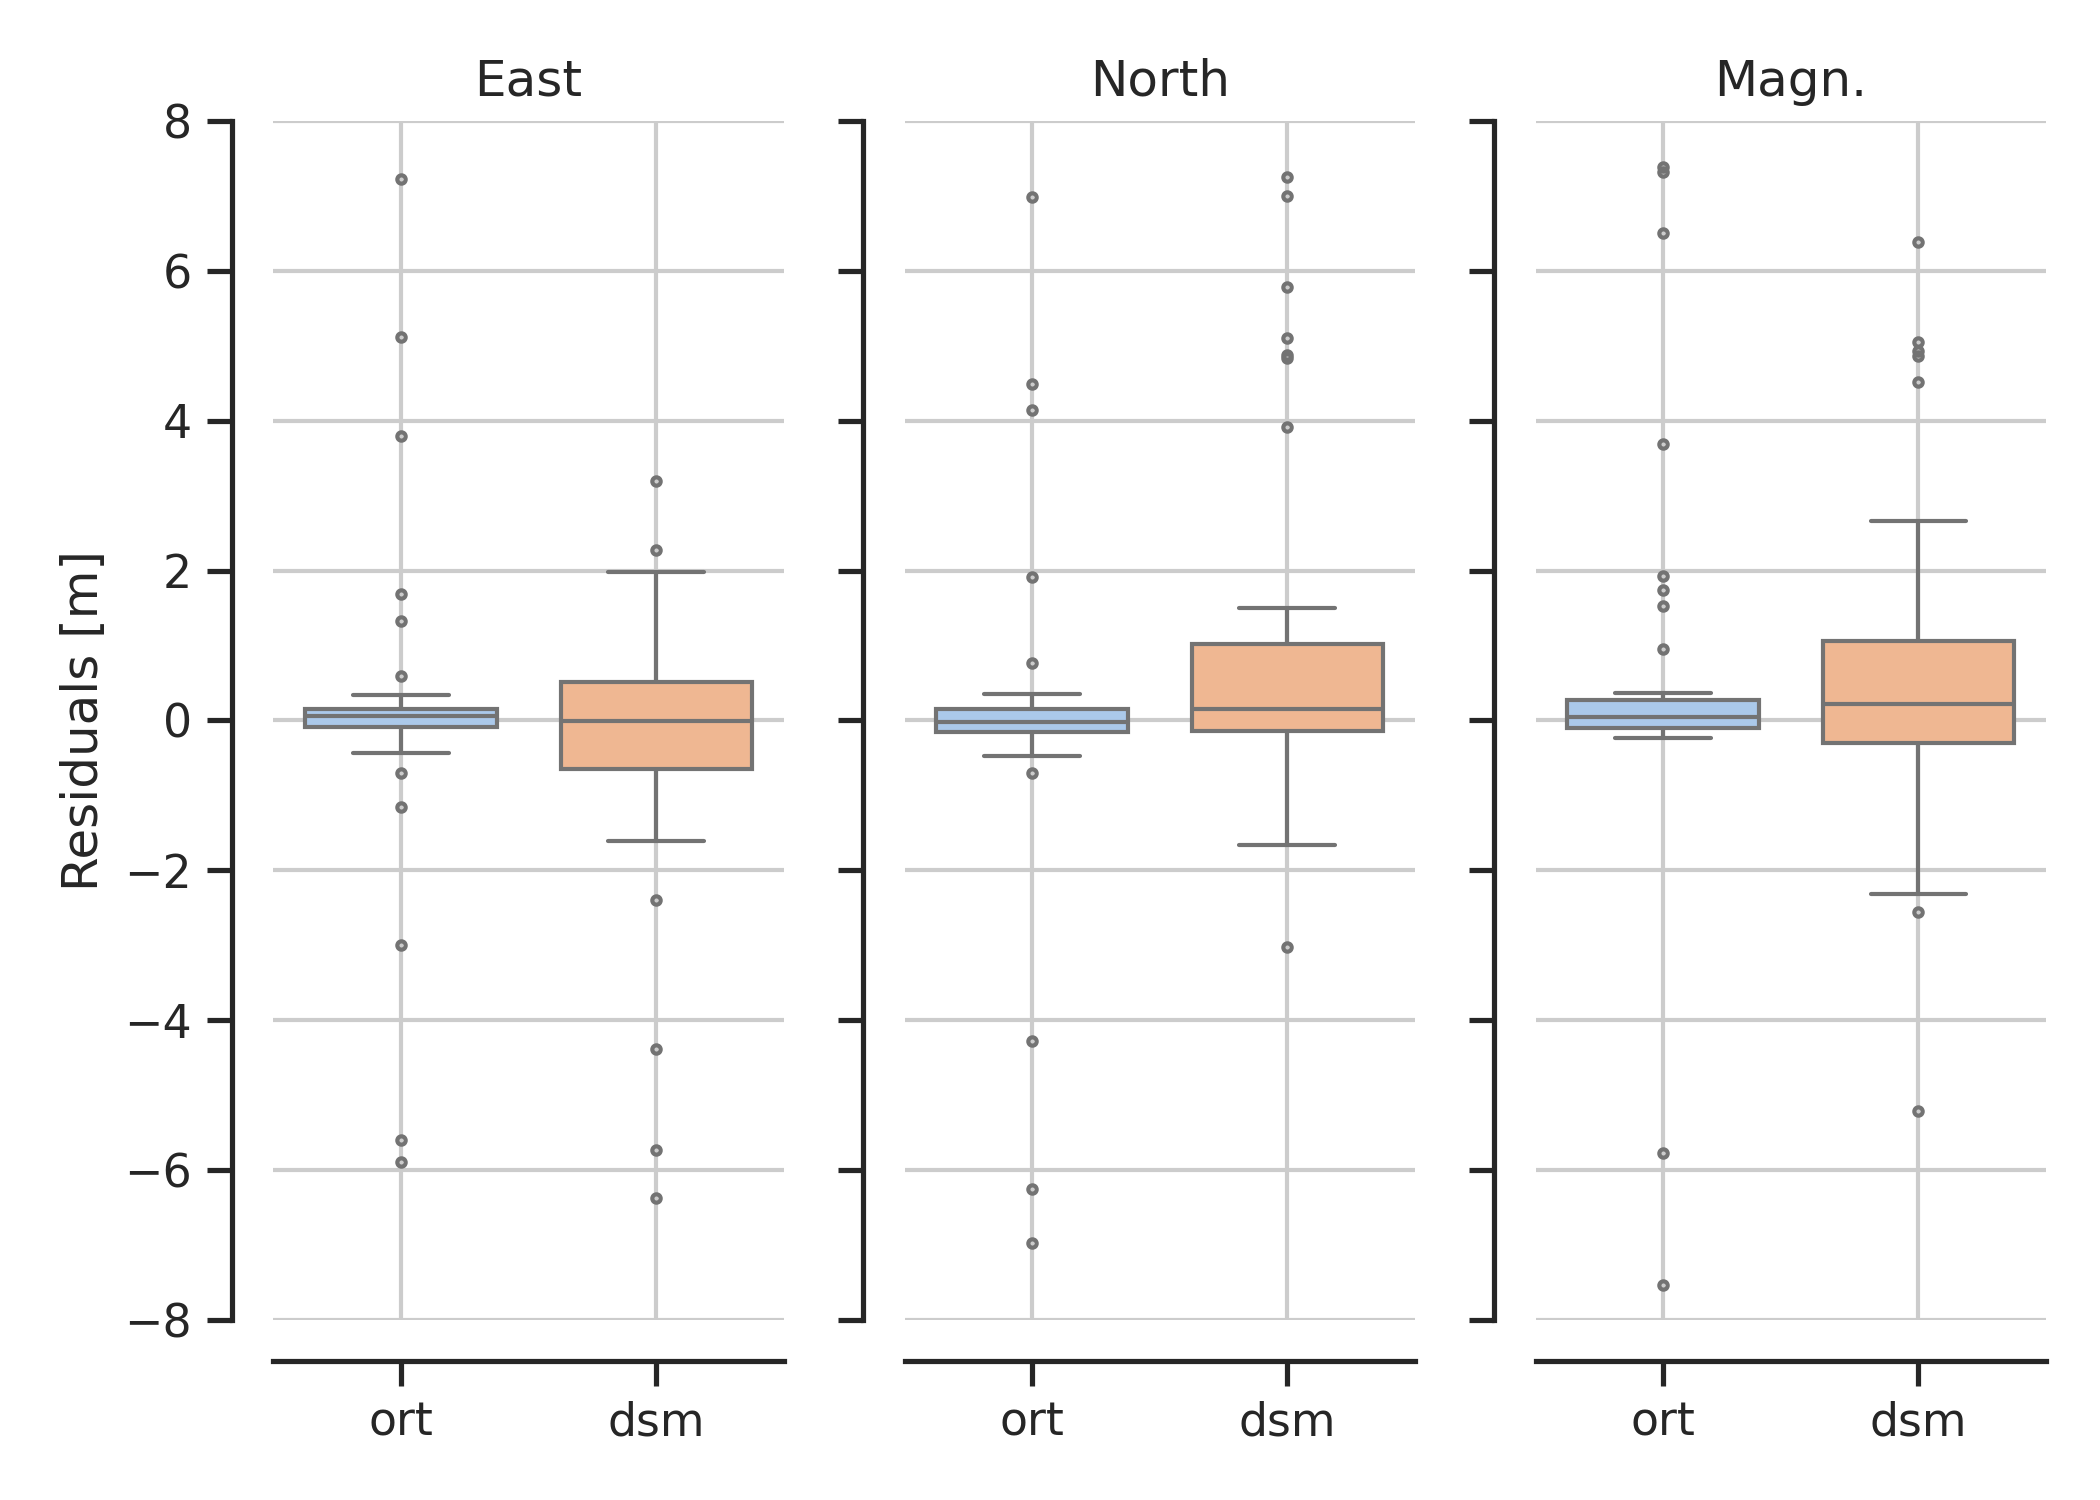
\includegraphics[width=0.8\columnwidth]{gps_lamma_boxplot.png}
    \caption{Boxplots of the differences between the displacements computed by GNSS measurements and those obtained by DIC on DSMs (from 2015 to 2018) and orthophotos (from 2018 to 2023). The differences are grouped by the image source (orthophoto --\textit{ort} -- and DSM) and divided into the East and North components and the magnitude of the displacement vectors.}
    \label{fig:3:gps_lamma_boxplot}
\end{figure}

The velocities obtained with DIC were compared with those measured by GNSS.
To this end, pyLamma was employed to calculate displacements based on templates centered around GNSS-measured target coordinates each year. 
To ensure a reliable comparison, 23 measurements of points located in particularly troublesome glacier areas, such as those near crevasses or where other morphological changes disrupt the image coherence between two consecutive years upon which DIC relies, were excluded from the comparison.
Thus, a dataset of 106 GNSS measurements spanning the glacier was used to compute the differences in East and North directions and magnitude between GNSS and DIC displacement vectors.

Overall, the \ac{mad} of differences was \SI{0.20}{\meter}, \SI{0.18}{\meter}, and \SI{0.22}{\meter} for East, North, and magnitude components, respectively.
These values are comparable to the GSD of the orthophotos and DSMs, highlighting an overall accuracy in displacement estimation at the pixel level.
Boxplots in \figref{fig:3:gps_lamma_boxplot} illustrate differences categorized by image source (DSM or orthophotos). 
While both groups show outliers exceeding \SI{2}{\meter}, orthophotos yield significantly less dispersion than DSMs.
Considering the magnitude of the displacement vectors, MAD for orthophotos was \SI{0.17}{\meter}, contrasting with DSM's three times larger \SI{0.58}{\meter}, highlighting a more robust performance of DIC on orthophotos compared to DSMs. 
Despite the challenges posed by snow partially covering the glacier and critical illumination conditions that forced the use of DSMs, the glacier surface displacement field was successfully computed by DIC for the period between 2015 and 2018, albeit with a coarser accuracy.

\begin{figure}[ht]
    \centering
    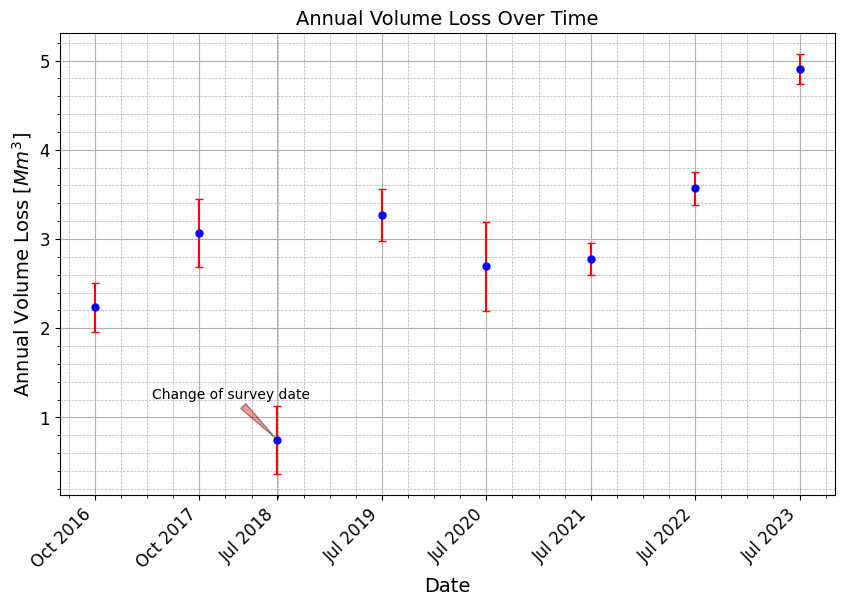
\includegraphics[width=1\columnwidth]{volume_loss_2015-2023.png}
    \caption{Yearly volume variation computed as the difference between DSM of consecutive years. The error bars represent the uncertainty of each value.}
    \label{fig:3:volumes}
\end{figure}

\subsection{Volume variations}\label{sec:3:res:volumes}

\begin{figure}[p]
  \centering
  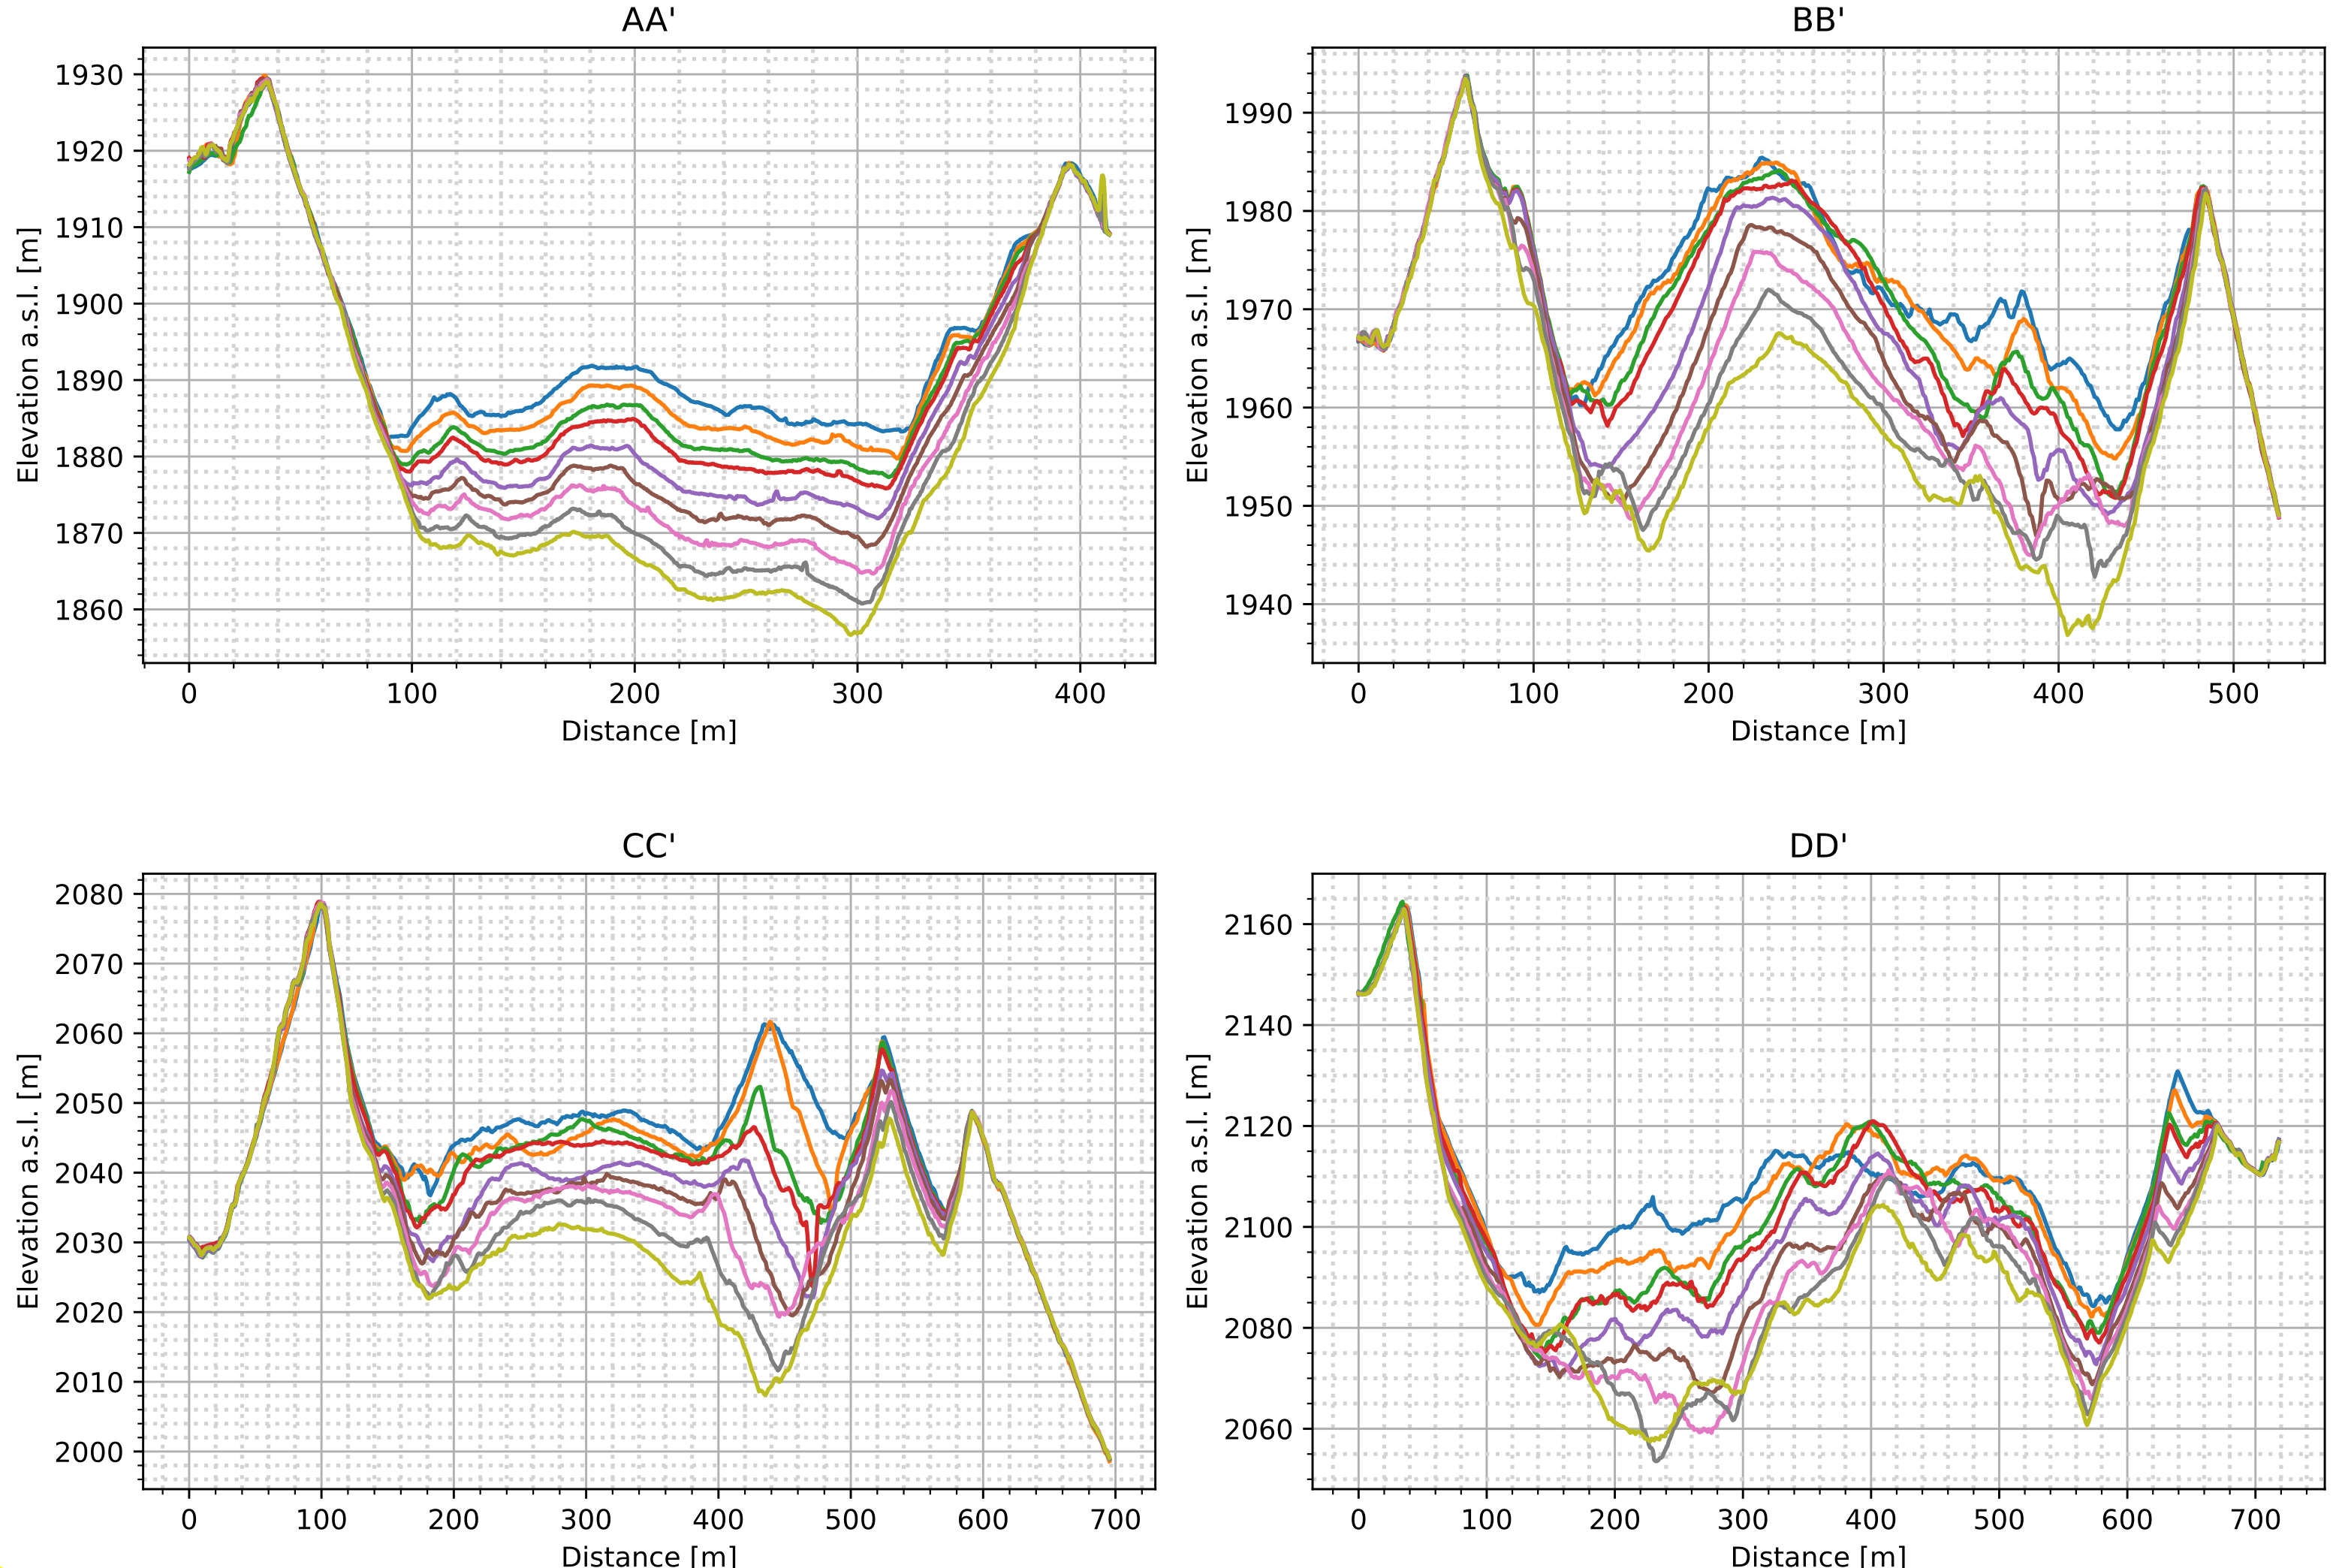
\includegraphics[width=\textwidth]{profiles.png} \\
  \subcaptionbox{\label{fig:3:profiles:profiles}}{
    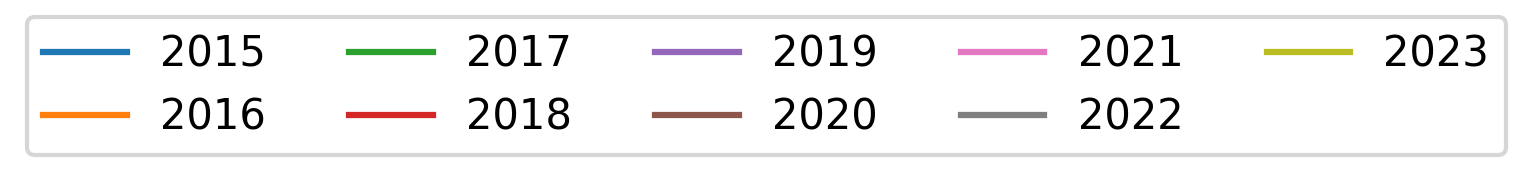
\includegraphics[width=0.55\textwidth]{profiles_legend.png}
  } \\
  \subcaptionbox{\label{fig:3:profiles:map}}{
    \includegraphics[width=.45\textwidth]{profiles_map.png}
  }
    \caption{\textbf{(a)} Elevation profiles obtained from the DSM computed for the years 2015-2023 along four different cross-sections. \textbf{(b)} Location of cross-sections. Cross-sections are viewed from south to north.}
    \label{fig:3:profiles}
\end{figure}

\begin{figure}[ht]
  \centering
  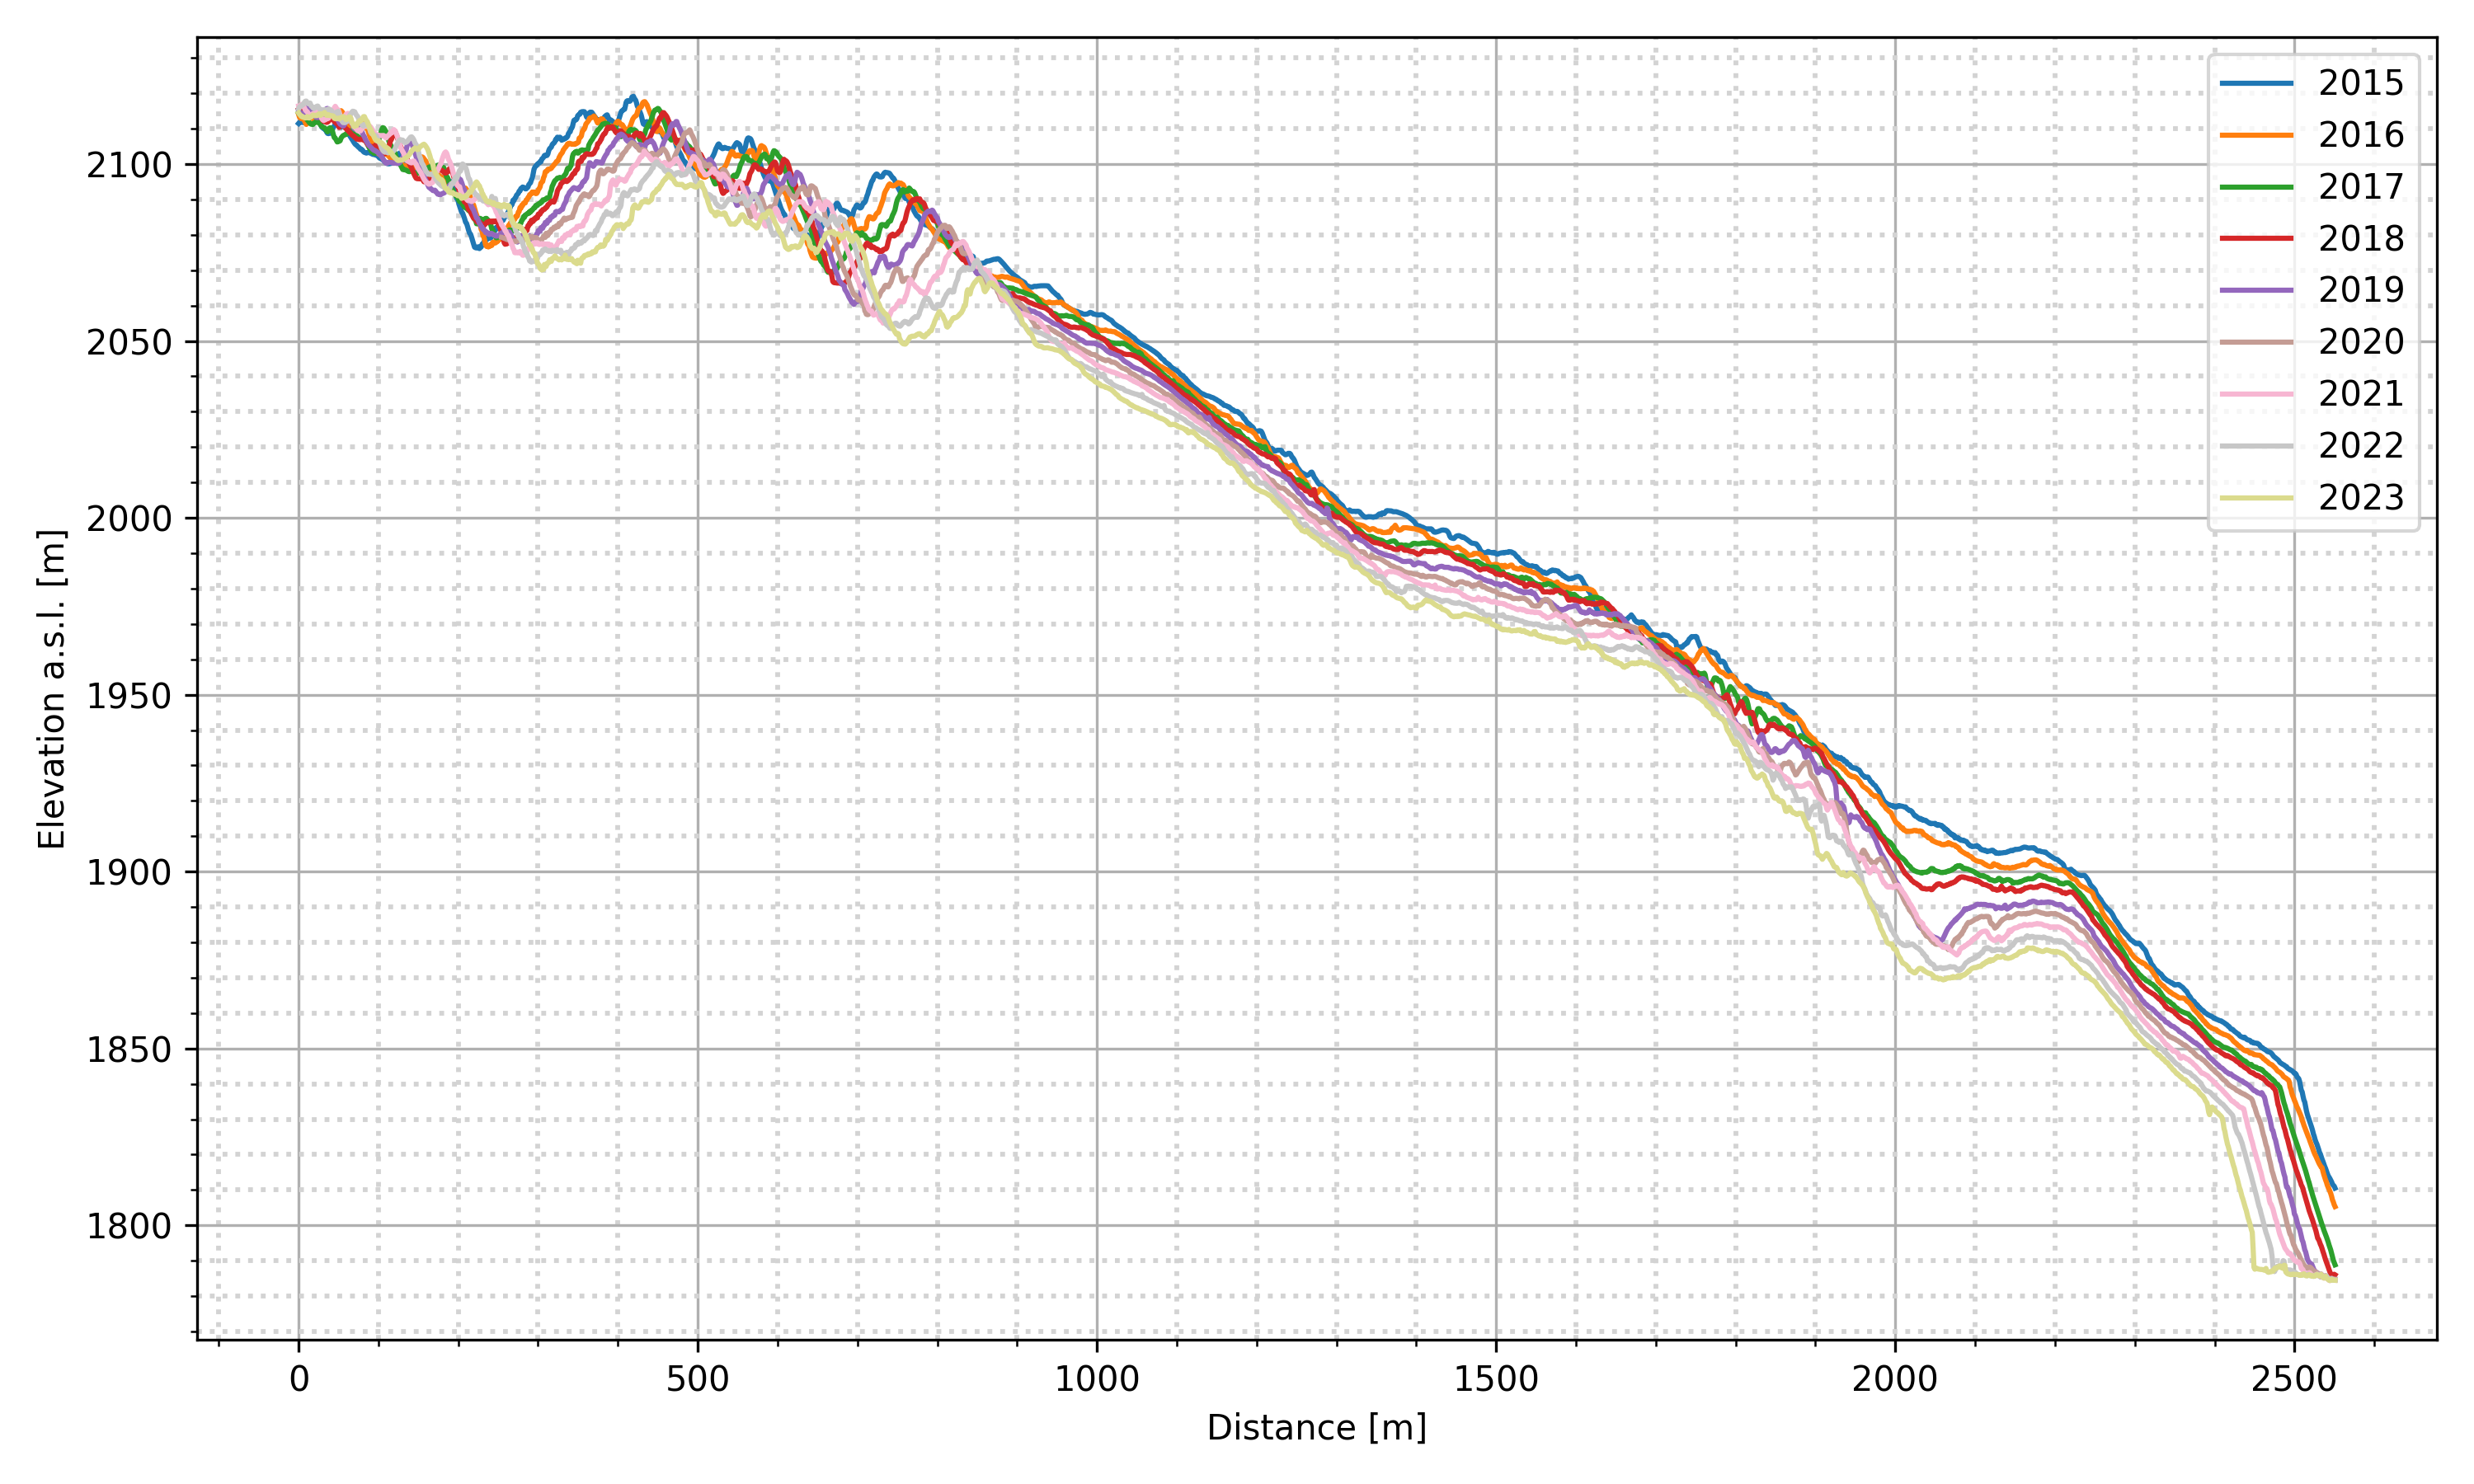
\includegraphics[width=\textwidth]{longitudinal_profiles.png}
  \caption{Longitudinal profiles of the glacier extracted each year along the centerline. The location of the profile is marked in \figref{fig:3:profiles:map}.}
  \label{fig:3:profile_long}
\end{figure}

\figref{fig:3:volumes} shows the annual ice volume loss for the glacier, with error bars indicating the estimated uncertainty in volume change (details in Section~\ref{sec:3:method_volumes}).  
On average, the glacier lost about \SI{3.21e6}{\cubic\meter}  of ice per year between 2015 and 2023. 
Notably, the time series reveals a concerning trend: ice loss is accelerating, with a non-linear increase in volume reduction from 2020 to 2023.
In particular, the exceptionally hot and dry summer of 2022 left a significant mark, resulting in a notable volume loss of \SI{4.90e6}{\cubic\meter} during 2022--2023.
These findings align with those observed in other alpine glaciers, such as the Mont Blanc glaciers \citep{Berthier2023b_exceptional_thinning}.

Due to the transition of fieldwork from Autumn to Summer between 2017 and 2018, the volume loss computed from October 2017 to July 2018 primarily reflects wintertime and springtime variations.
Therefore, it can not be directly compared with the annual average estimated for the other years.
Moreover, ice volume loss for 2019--2020 might be marginally underestimated due to significant geometric discrepancies in the photogrammetric model of the glacier's upper portion, attributed to the absence of GCPs measured in situ during photo acquisition. 

Excluding the period of 2017--2018, the year with the least ice ablation occurred between 2015 and 2016, amounting to \SI{2.23e6}{\cubic\meter}, while ice ablation peaked during 2022-2023
This trend emphasizes the sensitivity of glacier systems to climate variations and the need for continued monitoring to understand the evolving dynamics of glacial environments.

\figref{fig:3:profiles} presents elevation profiles of the glacier obtained annually at four distinct cross sections.
The series of cross-section AA' extracted at the northern terminal lobe (\figref{fig:3:profiles}a) shows a regular decrease in the glacier thickness
ice loss rate of approximately \qty{2}{\meter\per\year}.
In the other sections situated in the central and upper parts of the glacier (sections BB', CC', and DD', \figref{fig:3:profiles}b-d), 
the height reduction displays less regularity owing to the presence of crevasses.
Moreover, the formation of local peaks and valleys within the debris, arising from locally different melting processes, significantly disrupts the glacier's transfer zone. 
These features are particularly noticeable in the cross-sections BB' and DD'.
Notably, the glacier's streamwise right moraine experiences progressive sliding processes and collapses due to the diminishing support of the thinning glacier. 
This phenomenon is prominently observed in sections AA' and DD'.

\figref{fig:3:profile_long} shows the evolution of the glacier's elevation profile along its centerline from 2015 to 2023.
The most striking feature is the pronounced decrease in elevation near the heavily crevassed area separating the central body of the glacier from the northwestern terminal lobe (about 2000 m along the profile).
There is a progressive increase in surface slope here, reflecting the recent formation of irregular valleys with steep ice cliffs. 
This has led to an increasingly chaotic distribution of debris cover, which has intensified in recent years. 
In addition, the profiles show a gradual downslope movement of the irregular ice mass accumulation in the upper glacier. 
Finally, the glacier's terminal ice cliff experienced a significant retreat of about 200 meters between 2015 and 2023.

\section{Glacier mass variations from 1977 to 2023}

\begin{figure}[ht]
  \centering
  %   \subcaptionbox{\label{fig:3:cumulative_volumes_mass:volumes}}{
  %   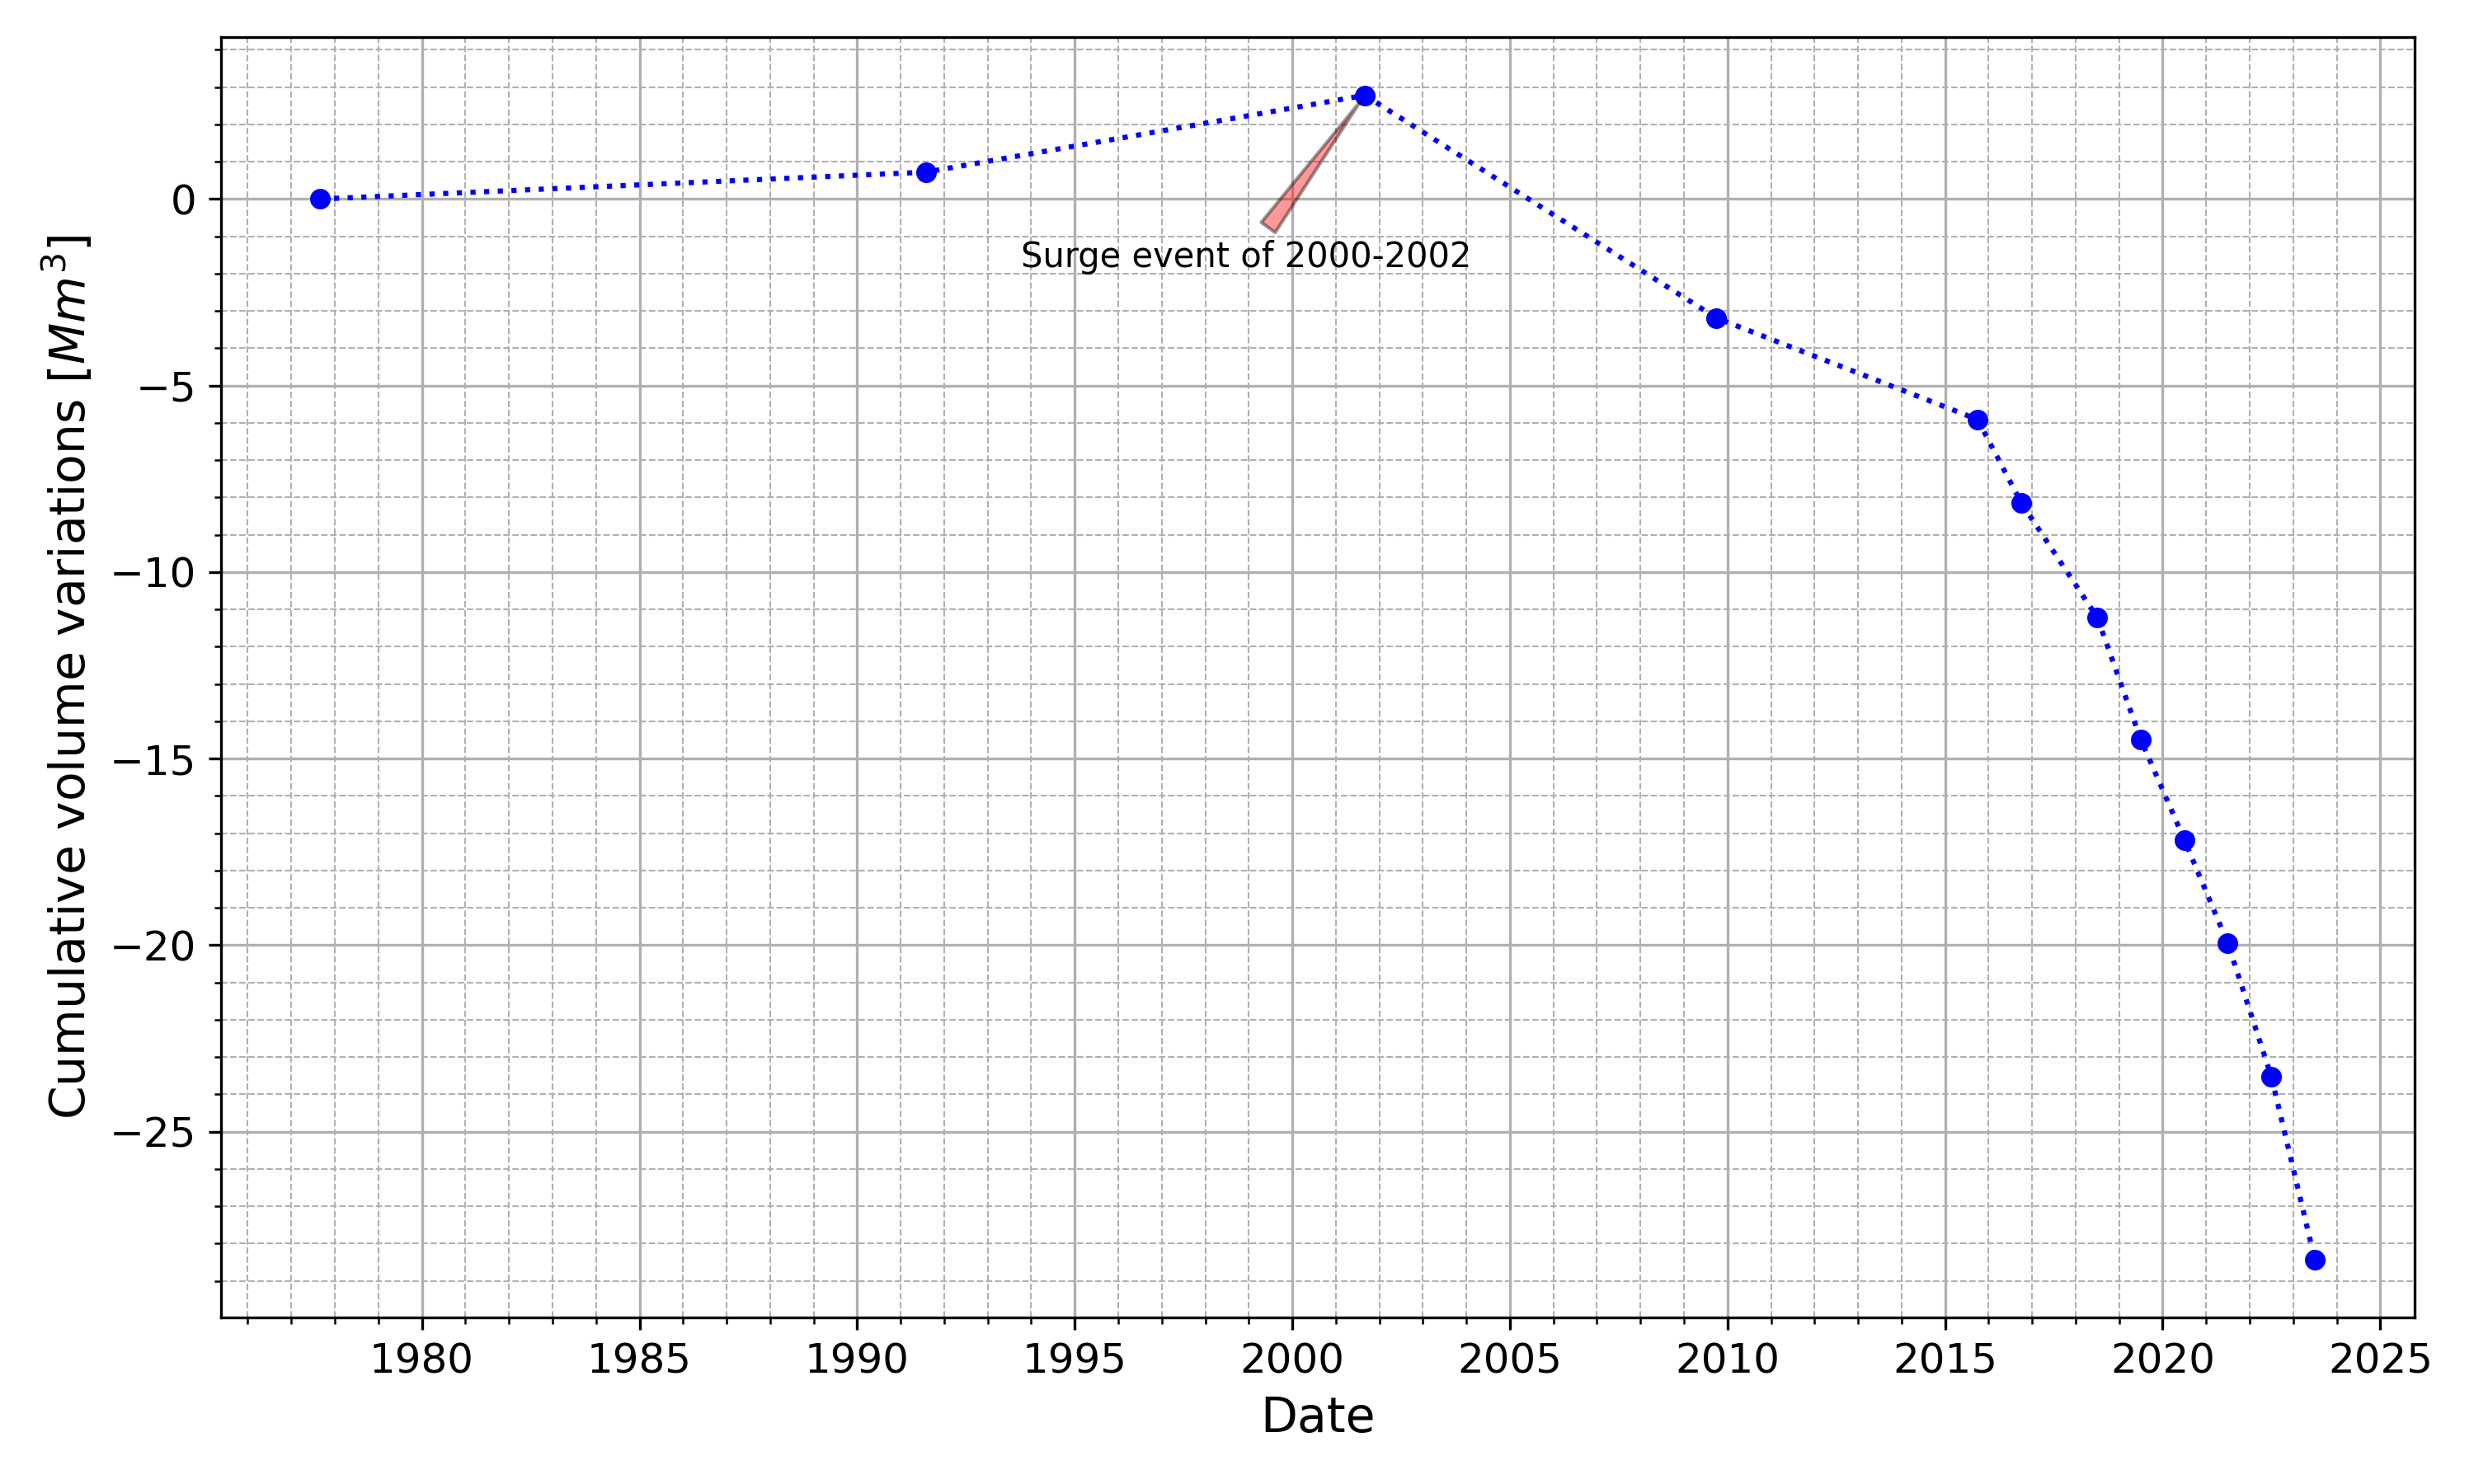
\includegraphics[width=0.8\textwidth]{cumulative_volume_variations_all.png}
  % } \\
  % \subcaptionbox{\label{fig:3:cumulative_volumes_mass:mass}}{
    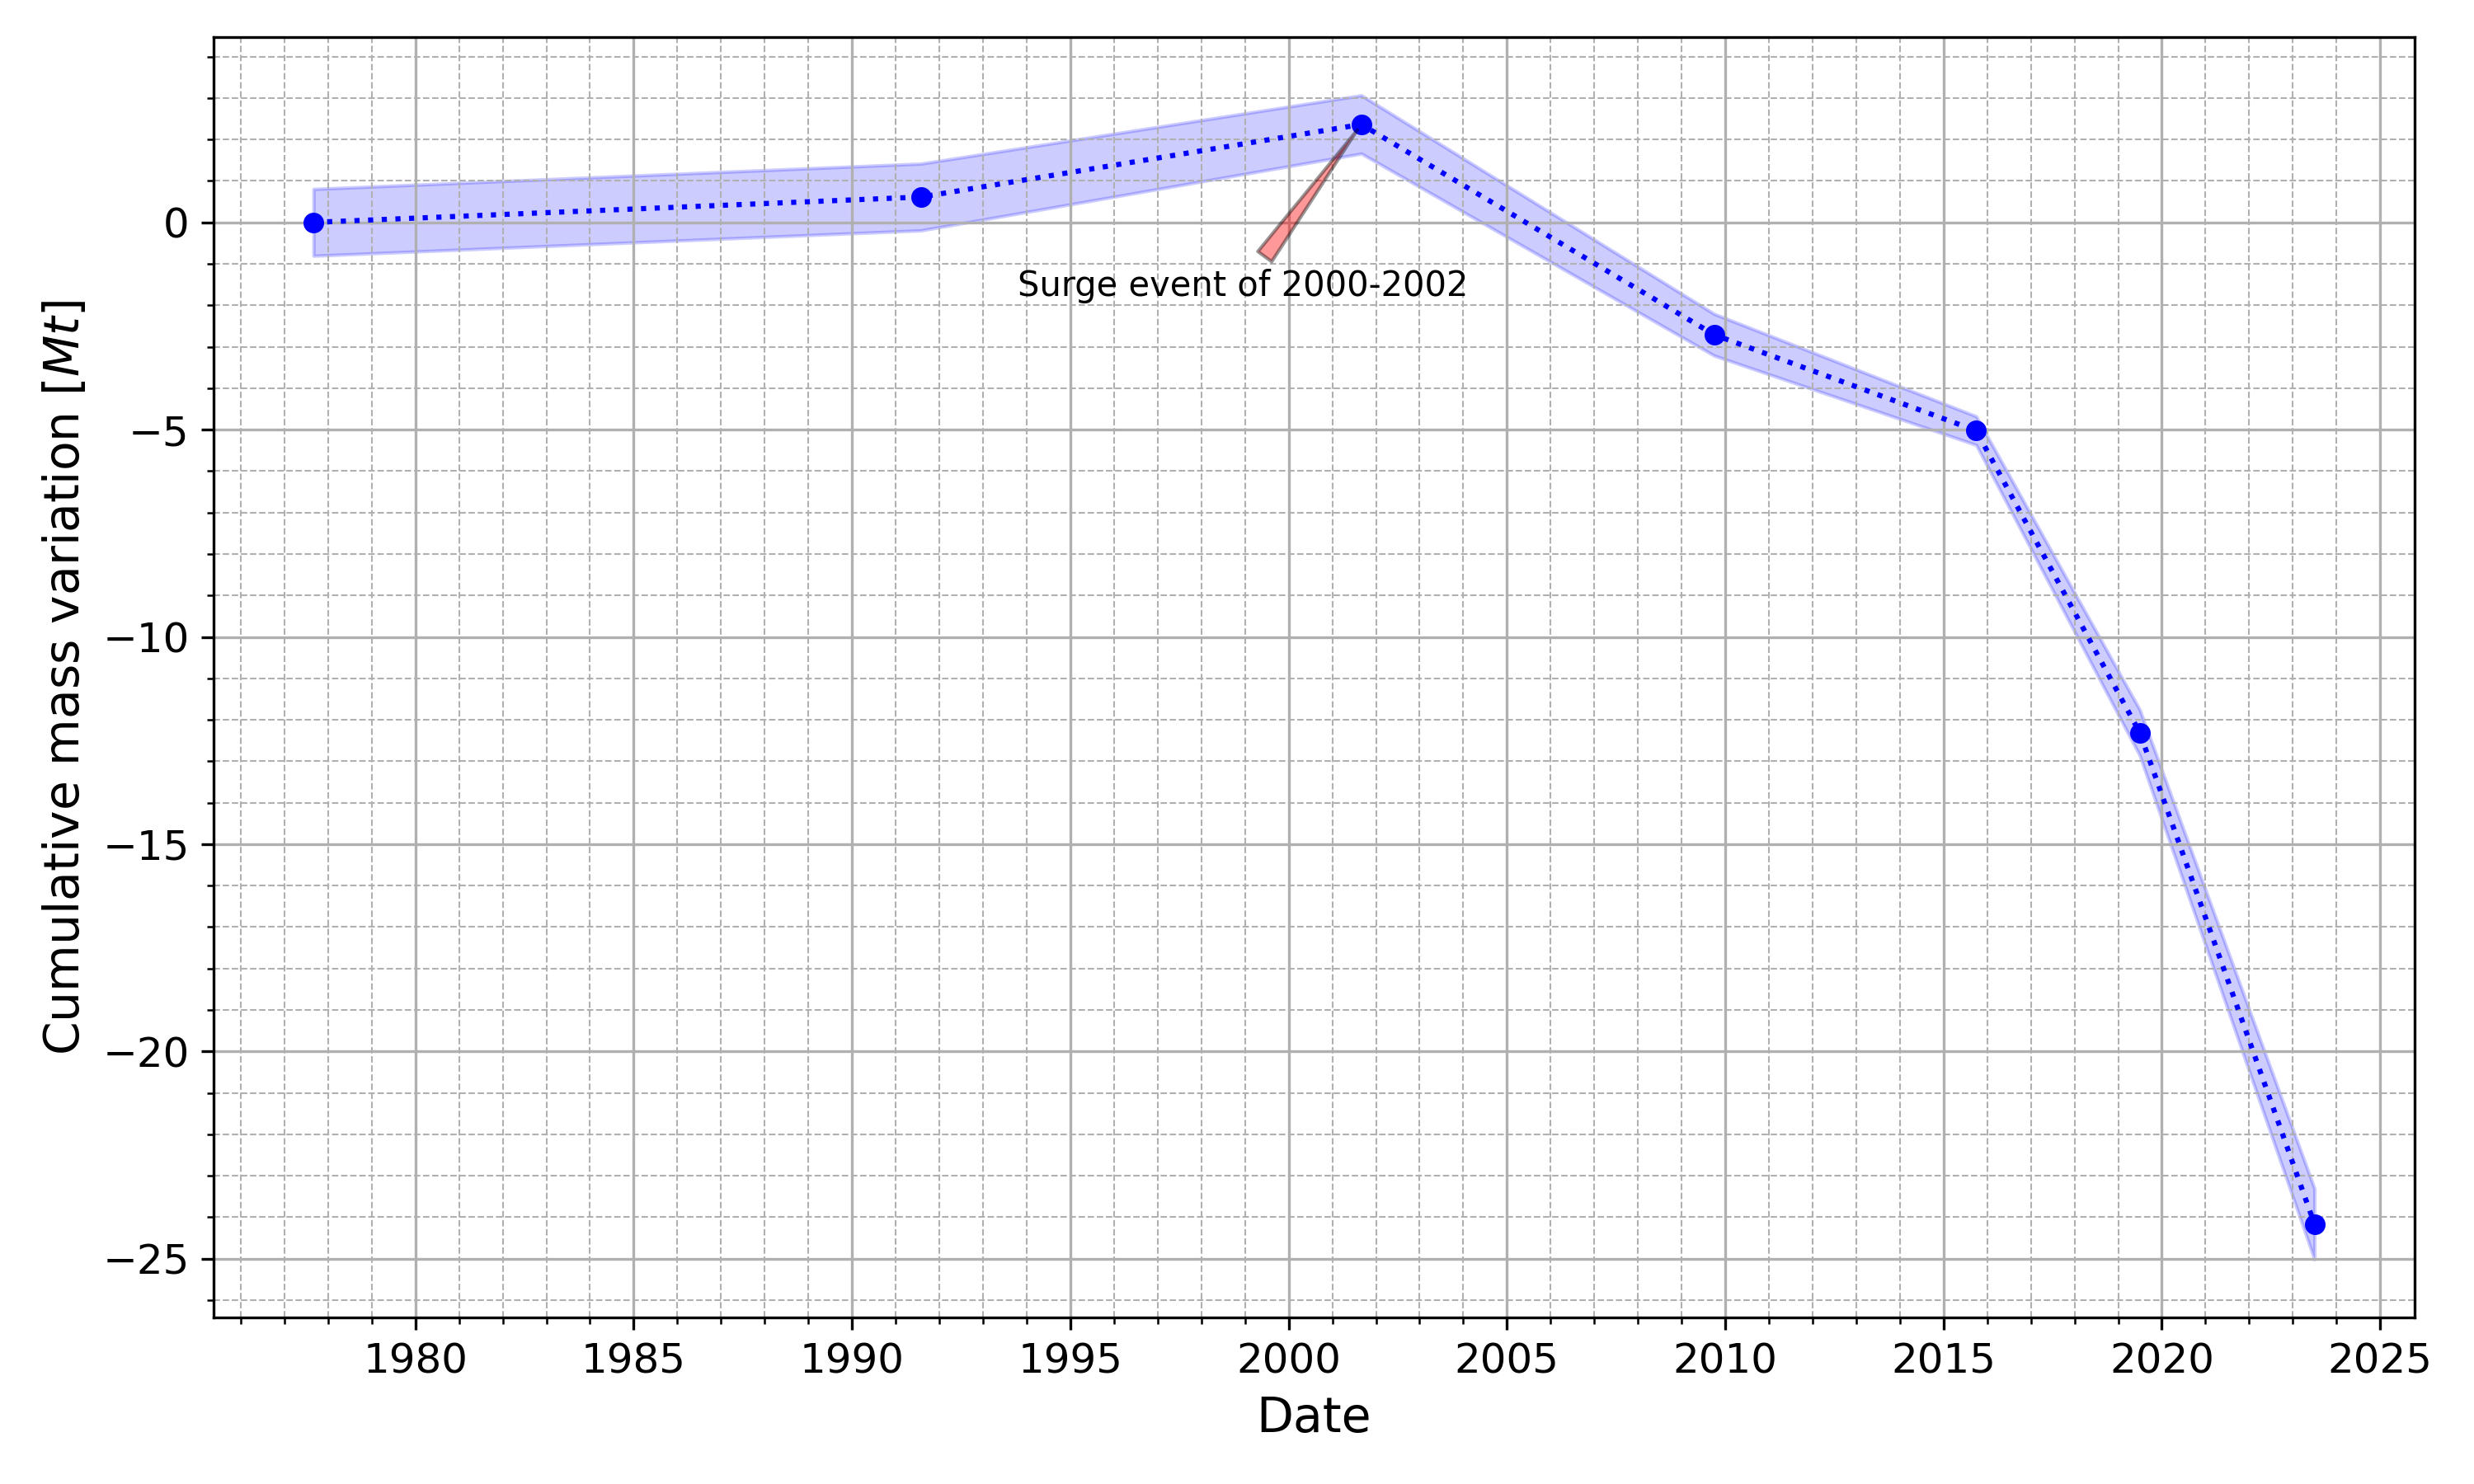
\includegraphics[width=\textwidth]{cumulative_mass_changes_all.png}
  % }
    \caption{(a) Cumulative volumes variations Belvedere Glacier (1977-2023) with 1977 as the reference year (b) Cumulative ice mass variations (in megatonnes), assuming an ice density of \SI[separate-uncertainty = true]{850 \pm 60}{\kilo\gram\per\cubic\meter}, considering periods longer than 5 years \cite{Huss2013_density_geodetic_balance}. % \textcolor{red}{Make again computation volume differences for the period 2015-2023}
    } 
  \label{fig:3:cumulative_volumes_mass}
\end{figure}

By integrating historical aerial surveys (chapter \ref{ch:2}) with repeated in-situ UAV measurements, this study quantified long-term cumulative volume changes in Belvedere Glacier from 1977 to 2023.
To convert volume variations into mass changes, an average ice density of \SI[separate-uncertainty = true]{850 \pm 60}{\kilo\gram\per\cubic\meter} was assumed \citep{Huss2013_density_geodetic_balance}. 
However, as emphasized in \citet{Huss2013_density_geodetic_balance}, this constant density assumption is only reliable for geodetic mass balance assessments over periods longer than five years.
Shorter intervals (< 3 years) introduce significant uncertainty due to potential density variations within the firn layer.
To address this, geodetic mass balance calculations focused on three UAV surveys spaced approximately five years apart (2015, 2019, 2023) in addition to the previous aerial surveys.  

\figref{fig:3:cumulative_volumes_mass} shows the estimated mass variations.
The Belvedere Glacier increased in mass from 1977 to 2001, highlighting its expansion period. 
This trend abruptly ended with the 2000-2002 surge event, resulting in a significant mass gain around 2001. 
Subsequently, the glacier has undergone a continuous and dramatic retreat. 
As of 2023, the Belvedere Glacier has lost \SI{\sim 24}{\mega\tonne} of ice mass compared to its 1977 state.

\section{An open-source framework for sharing monitoring results}\label{sec:3:open-data}

The long-term monitoring campaign of Belvedere Glacier has produced a rich dataset that includes high-accuracy in-situ GNSS measurements, 3D point clouds, DSMs, and orthophotos derived from UAV photogrammetry.
In recognition of the value of collaboration and open science, all point clouds, DSMs, and orthophotos for the entire glacier have been made publicly available under the GNU General Public License (GPL) version 3 license through a Zenodo repository\footnote{Belvedere Open Data: \url{https://doi.org/10.5281/zenodo.7842347}}~\citep{ioli_2023_zenodo}.
All data are accompanied by a structured JSON file containing essential metadata, which allows researchers to use the data efficiently and encourages further scientific exploration by researchers across disciplines.
This will allow replication of the analyses performed in this thesis, such as estimates of glacier velocity and volume change, and facilitate the study of other geomorphological processes, such as moraine collapse, or derive new insights into glacier dynamics. 

To maximize accessibility for non-expert users, the 3D point clouds derived from all the surveys were converted to a Potree-compatible structure \citep{schutz2016potree} and uploaded to a web server.
Potree is an open-source WebGL-based JavaScript library designed for web-based rendering of large-point clouds, and it offers versatile tools for handling 2D and 3D objects, scene navigation, and interaction, including measurements and cross-section profile extraction~\citep{Gaspari2024, Fascia2024}.
The 3D glacier models are accessible from any web browser (\figref{fig:3:potree}), allowing users to navigate through different years and experience the evolution of the glacier over time\footnote{Potree web app: \label{the-belvedere-glacier-website}\url{https://thebelvedereglacier.it/potree/index.php}}.
\marginpar[Note 1]{
    
\includegraphics[width=\marginparwidth]{qr_thebelvedereglacier.png}
}

\begin{figure}[p]
  \centering
    \subcaptionbox{\label{fig:3:profiles:potree:viewer}}{
    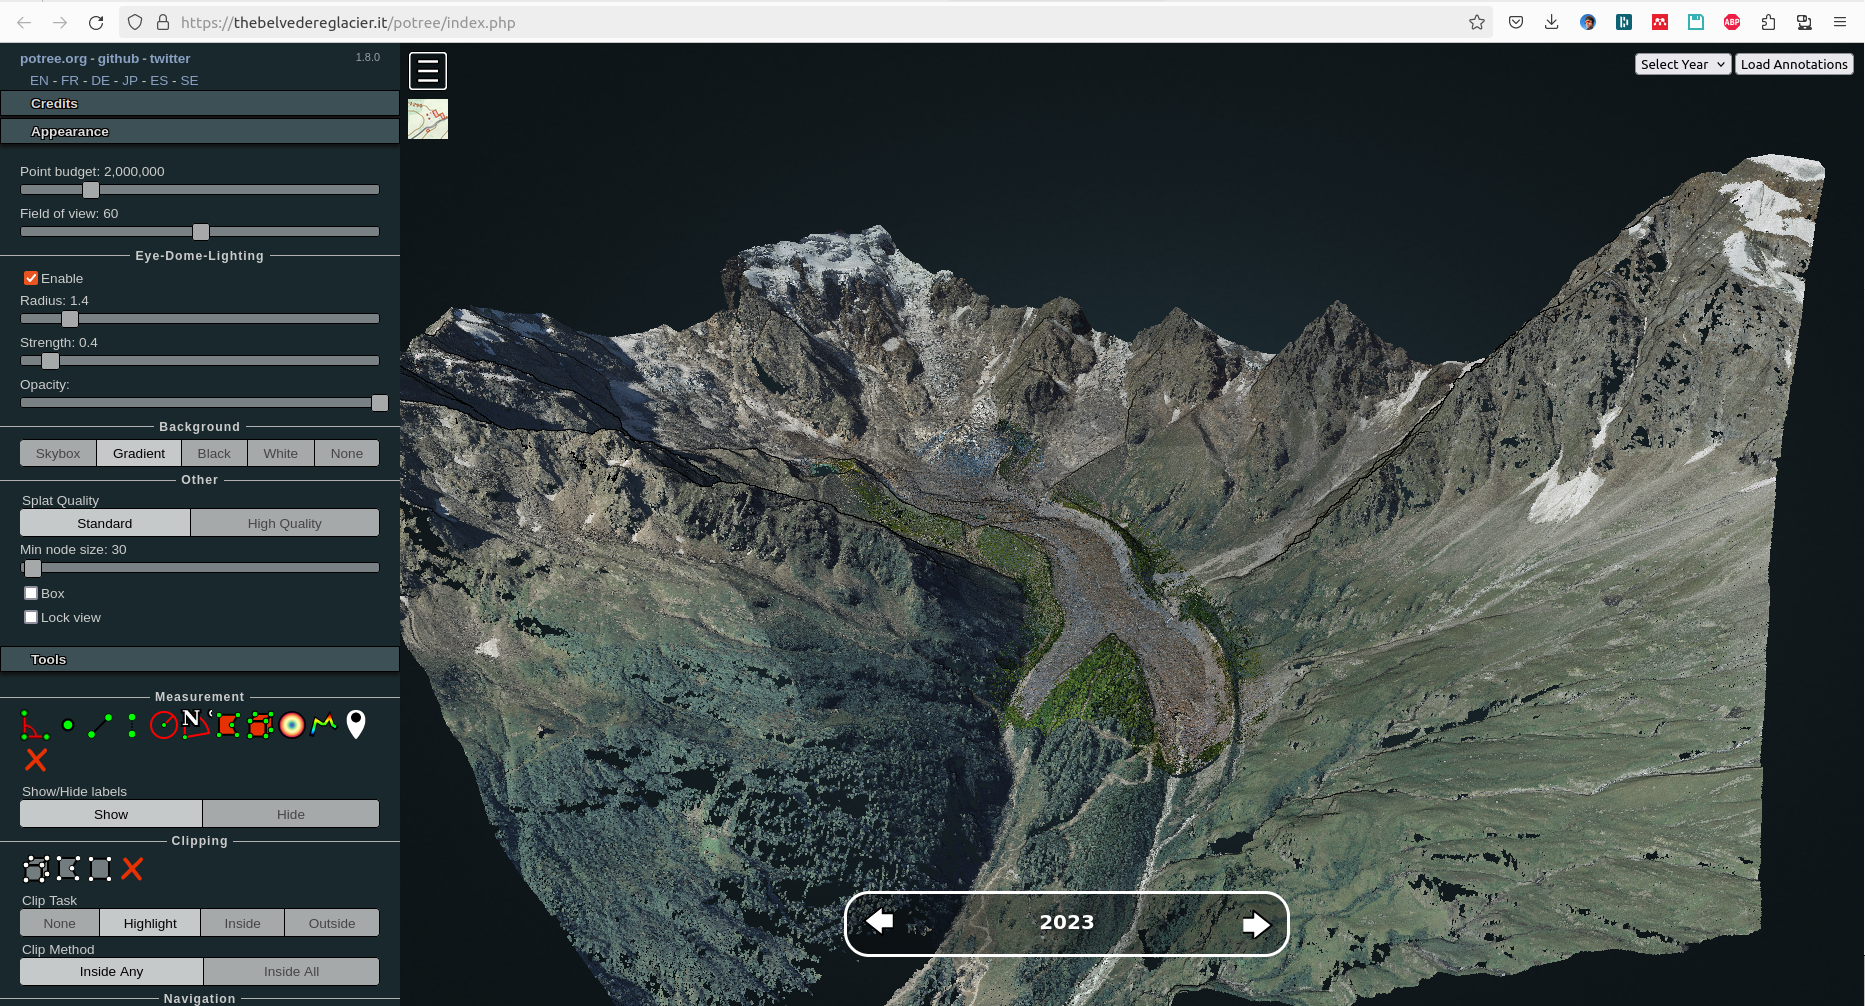
\includegraphics[width=0.95\textwidth]{potree_viewer.png}
  } \\
  \subcaptionbox{\label{fig:3:profiles:potree:sections}}{
    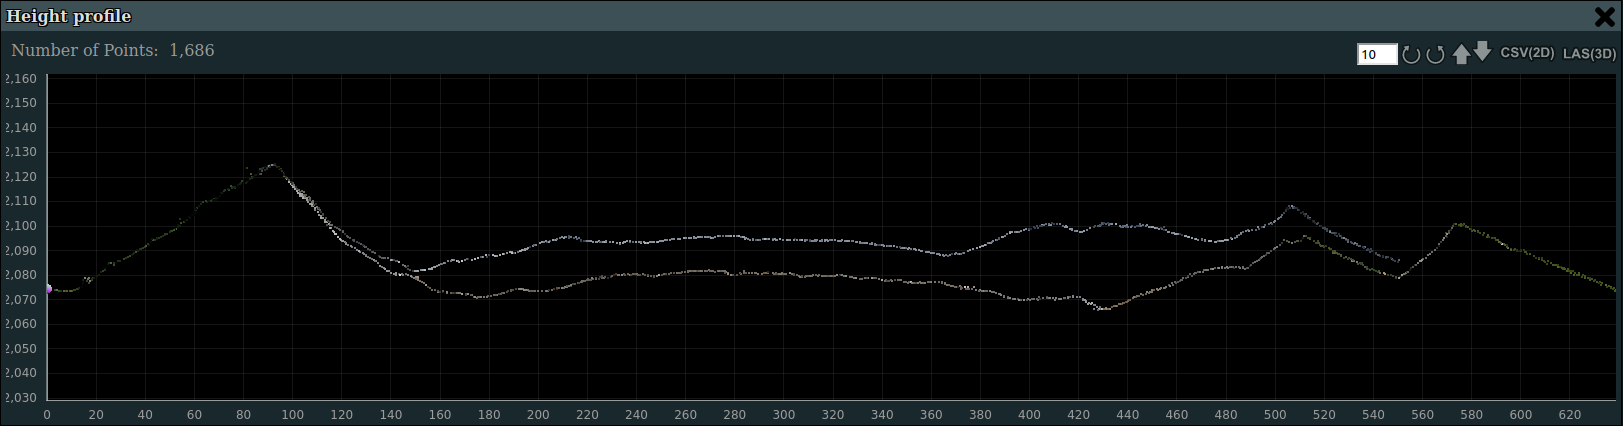
\includegraphics[width=.95\textwidth]{potree_sections.png}
  }
    \caption{\textbf{(a)} Web platform based on Potree \citep{schutz2016potree} for exploring the photogrammetric point clouds of the Belvedere Glacier acquired during the different surveys. \textbf{(b)} Example of two cross sections extracted directly from the Potree web interface from the point clouds of 2023 and 2015 to easily estimate the glacier thinning.}
    \label{fig:3:potree}
\end{figure}

Additionally, a robust open-source relational database serves as the central repository for the monitoring campaign's outcomes, ensuring easy storage, use, and sharing. 
We chose PostgreSQL for its flexibility, permissive open-source license, and seamless ability to manage geospatial data through the PostGIS extension. 
Using a PostgreSQL database centralizes data storage, allows direct use within GIS software packages as well as remote public access (e.g., via a read-only web interface) while protecting sensitive internal data through customizable permission levels.
The database primarily serves as a repository for field survey data, including details such as survey dates, instrument specifications, key acquisition parameters, and selected processing statistics. 
It also contains periodic GNSS measurements of photogrammetric targets and outputs from photogrammetric processes, including DSMs, orthophotos, derived glacier velocities, and volume changes.

\begin{figure}[ht!]
  \centering
  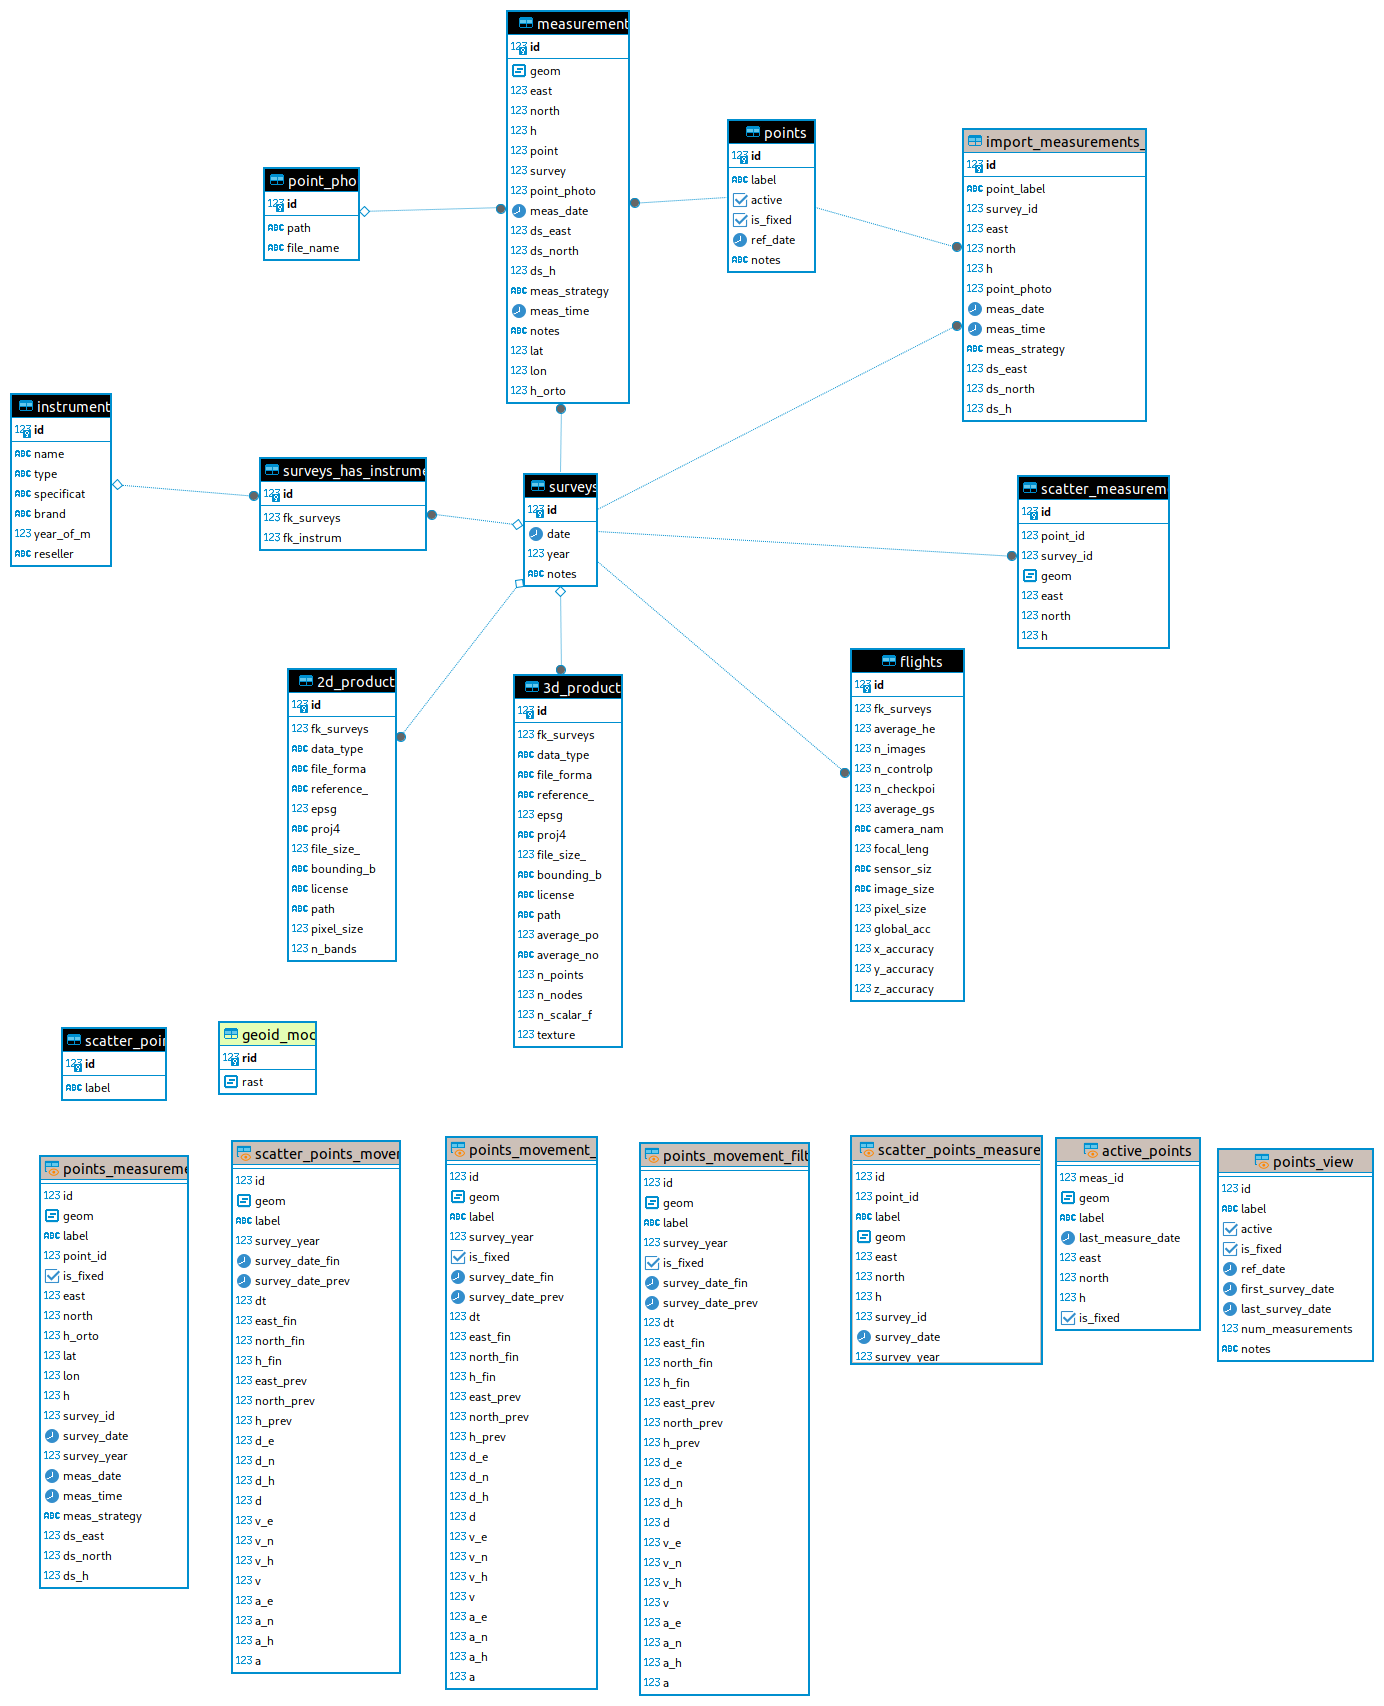
\includegraphics[width=\textwidth]{belvederedb_erd.png}
  \caption{ERD diagram of the PostgreSQL database used for storing the Belvedere results.}
  \label{fig:3:belvederedb_erd}
\end{figure}

Following the principles of relational databases, data is structured across multiple tables, with access facilitated by defined relationships using primary and foreign keys. 
The logical model of the database, shown in \figref{fig:3:belvederedb_erd}, describes the main tables and their relationships.
Key components of the database include the \textit{surveys} table, which contains information about each survey; the \textit{points} table, which catalogs points that have been periodically GNSS surveyed; and the \textit{measurements} table, which contains the actual GNSS measured coordinates. 
Each measurement is associated with a survey record, which allows retrieval of survey timing and instrumentation information used to collect the measurement, and a point record, which associates the measurement with a specific point label, allowing tracking of points in time.
Each measurement can be associated with an image, stored in a separate table, to document the acquisition.
In the \textit{surveys} table, each survey is linked to its corresponding metadata stored in the \textit{instruments} table, which contains information on all instruments used over the years, and the \textit{flights} table, which includes details of each photogrammetric flight performed.
In addition, each survey is associated with the products derived from the photogrammetric processing.
This organizational structure streamlines data retrieval using SQL queries, enabling tasks such as extracting measurements from individual surveys or ranges of surveys and deriving displacement time series for specific points.

This structure defines the core of the database, which is intended for internal use. 
However, to improve accessibility and streamline data retrieval, a set of predefined queries has been used to create read-only views (i.e., read-only subsets of a database based on a query that runs on one or more tables) within a separate public schema. 
These views provide a higher level of abstraction and functions for accessing information such as the measured points for each year, identifying active points (i.e., targets still present on the glacier and not lost) by providing their most recent measurement, and automatically calculating a time series of displacements, velocities, and accelerations for each point by differentiating consecutive measurements.
Additional functionalities encompass the automatic conversion of GNSS coordinates from the geographic WGS84 reference system to the projected RDN2008 / UTM zone 32N reference system and vice versa. 
Furthermore, the database facilitates the computation of orthometric heights for each measurement via bilinear interpolation using the Italian Geoid model ITALGEO05~\citep{Barzaghi2007}.

The database currently stores 456 GNSS measurements from 85 distinct points measured across 19 surveys. 
Thanks to the PostGIS extension, information can be easily displayed on a map canvas in GIS software like QGIS, together with predefined visualization styles, facilitating visual analysis (\figref{fig:3:db_qgis_query}).
Furthermore, researchers and non-expert users can access the public schema of the database via a dedicated web platform\footnote{Web app \url{https://thebelvedereglacier.it}}. 
Here, users can effortlessly view the GNSS measurements on a web map, extract time-series information, and download them for their scientific inquiries. 
Combining this with a web-based visualization of the 3D point clouds with Potree gives a complete overview of the outcomes of the Belvedere Glacier monitoring campaign.

\begin{figure}[ht]
  \centering
  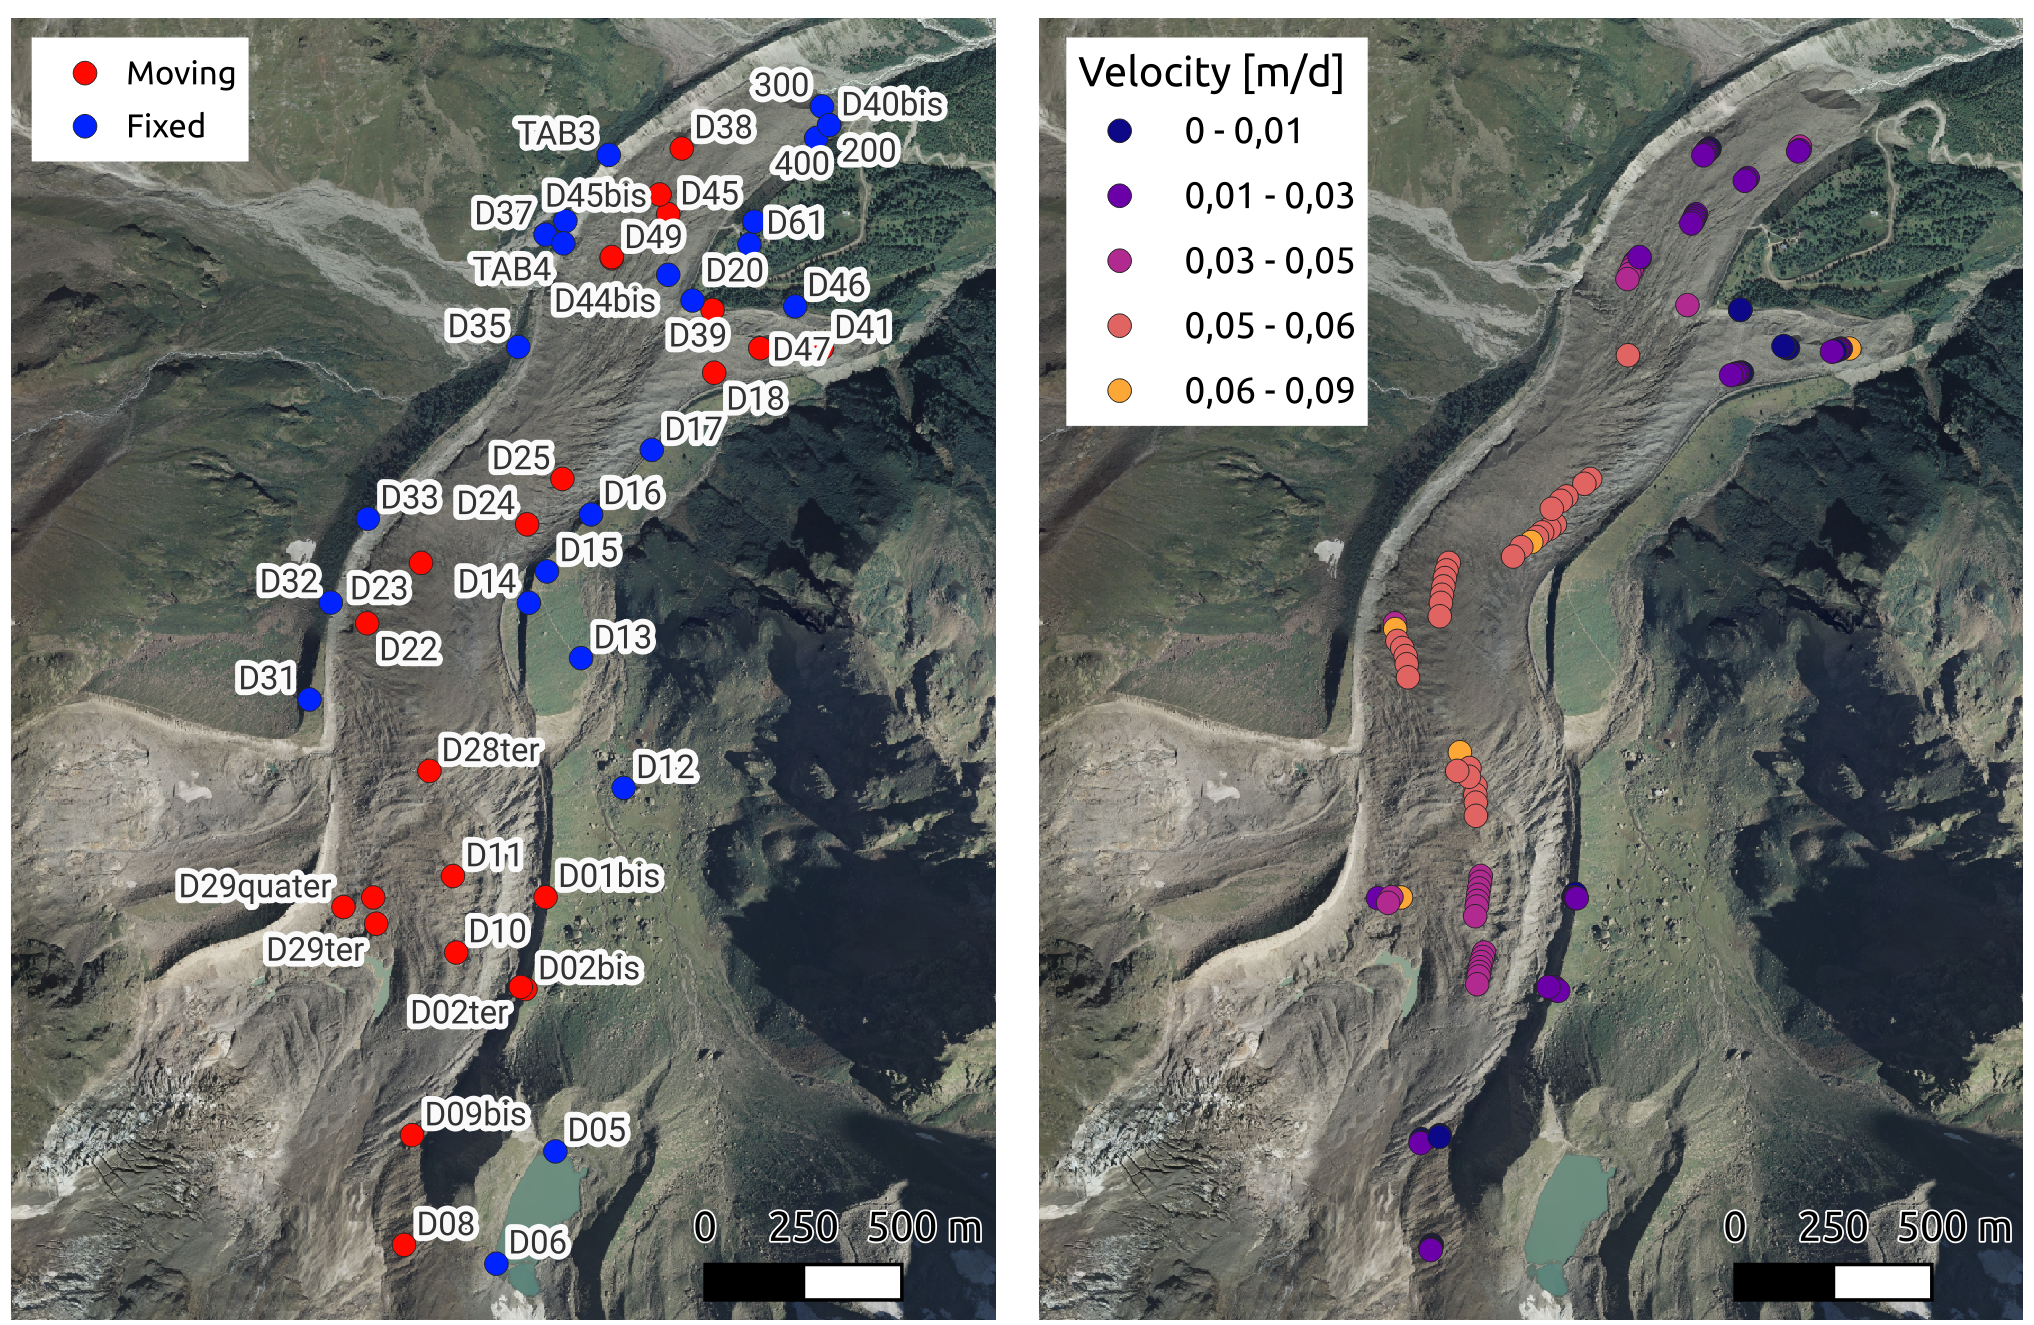
\includegraphics[width=0.9\textwidth]{db_qgis_query.png}
    \caption{Example of georeferenced layer queries from the PostgreSQL database using QGIS. The layer symbology is directly stored within the database and is automatically loaded into the QGIS project upon layer loading.}  
    \label{fig:3:db_qgis_query}
\end{figure}

% References
\makechapterbibliography{}


\graphicspath{{figures/chapter4/}}

\chapter{Deep learning low-cost photogrammetry for 4D short-term glacier monitoring
  (2022-2023)}

\vfill

\newthought{This chapter is based on:}

\begin{itemize}
  \item Paper under review on PFG
  \item Ioli, F., Bruno, E., Calzolari, D., Galbiati, M., Mannocchi, A., Manzoni, P.,
        Martini, M., Bianchi, A., Cina, A., De Michele, C., and Pinto, L. (2023). A
        REPLICABLE
        OPEN-SOURCE MULTI-CAMERA SYSTEM FOR LOW-COST 4D GLACIER MONITORING, Int. Arch.
        Photogramm. Remote Sens. Spatial Inf. Sci., XLVIII-M-1-2023, 137–144, \\
        \url{https://doi.org/10.5194/isprs-archives-XLVIII-M-1-2023-137-2023}
\end{itemize}

\newpage

\section{Introduction}\label{sec:4:introduction}

{\color{red} TODO: write introduction}

\begin{figure}
  \centering
  \subcaptionbox{\label{fig:4:studyarea:map}}{
    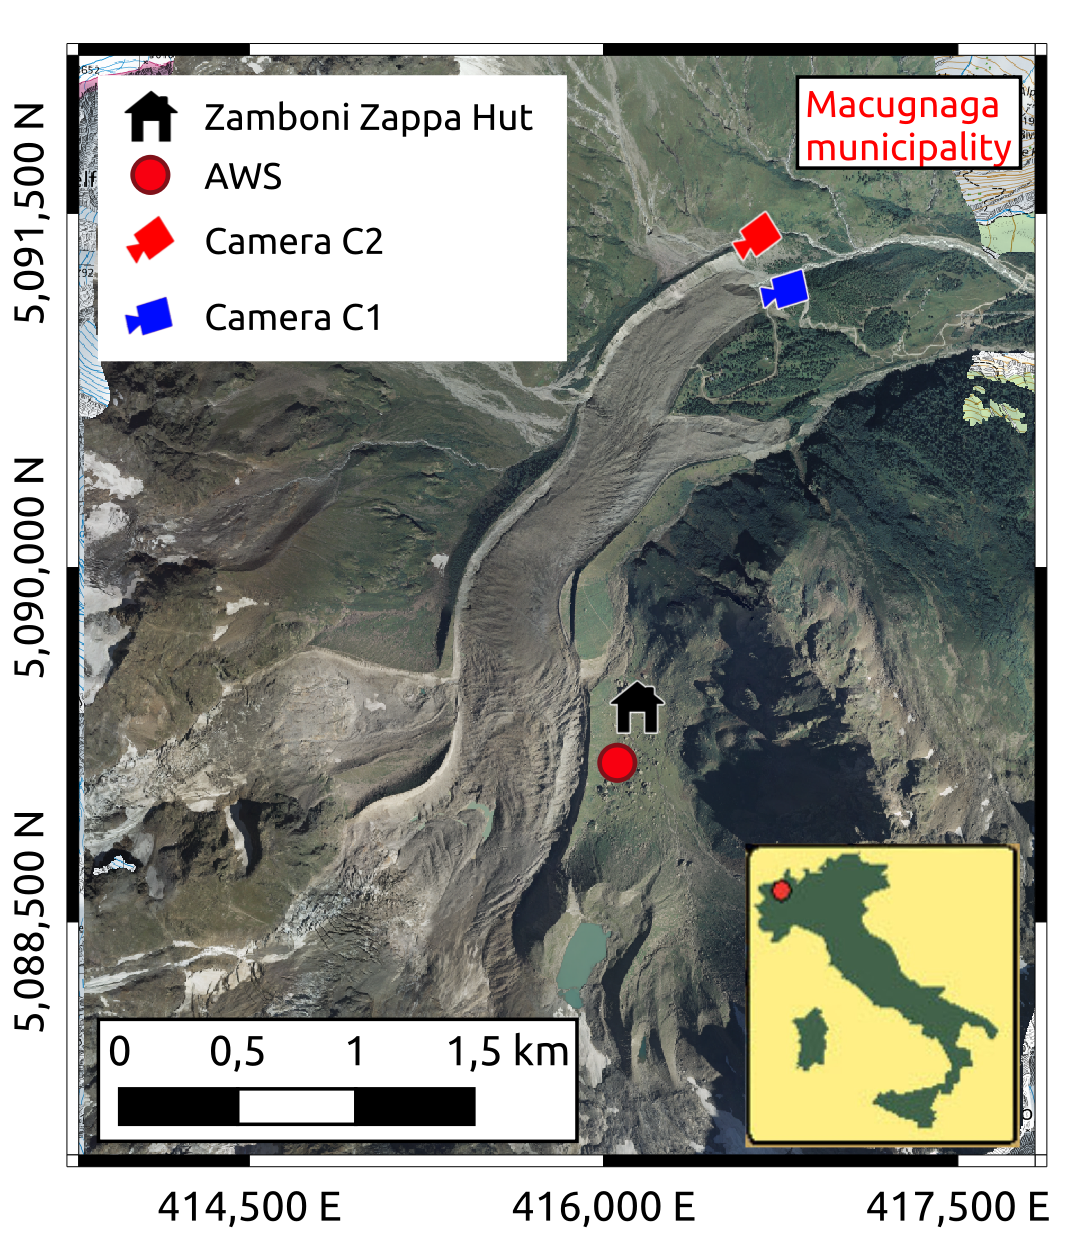
\includegraphics[width=.3\textwidth]{2_geographic_framework.png}
  }
  \subcaptionbox{\label{fig:4:studyarea:pic}}{
    \includegraphics[width=0.67\textwidth]{2_area_of_sudy.png}
  }
  \caption{(a) Map of the Belvedere Glacier, with marked the location of the two cameras
    C1 and C2, the Automatic Weather Station (AWS) and the Zamboni Zappa Hut;
    (b) The area of study: the stereoscopic reconstruction is focused on the terminal ice
    cliff (dashed light blue line), while the monoscopic DIC processing from camera C2
    image sequence is focused on the upper area of the north lobe (dashed green line).}
  \label{fig:4:studyarea}
\end{figure}

\section{The low-cost stereoscopic system}\label{sec:4:system}

% From last paper
The low-cost stereoscopic system consists of two autonomous and independent monitoring
units. Each unit is includes an off-the-shelf DSLR camera (Canon Eos 1200D), an Arduino
microcontroller for camera triggering, and a Raspberry Pi
Zero with a SIM card for sending images to a remote server via a GSM
network\citep{ioli2023_replicable}.
The instruments are housed in waterproof cases and mounted on tripods anchored to stable
rocks along the glacier moraines.
Power is supplied by a solar panel combined with a sealed lead-acid battery.
The total cost of each unit was less than \texteuro2000, including
camera and lens \citep{ioli2023_replicable}.
The low-cost camera system is described in detail in \citet{ioli2023_replicable}.

The two monitoring stations, labelled as C1 and C2, were installed in summer 2021 on
either side of the north tongue of Belvedere Glacier (\figref{fig:4:studyarea}).
The harsh glacier environment with steep and unstable moraines, often subject to rockfall
due to glacier retreat, constrained the camera installation location at
\SI{\sim230}{\meter} (camera C1) and \SI{\sim350}{\meter} (camera C2) from the terminal
ice cliff, with a strongly convergent pose.
Different lenses were used for the two cameras to achieve the same image scale in
correspondence of the glacier tongue: C1 was equipped with a 24 mm lens, while a 35 mm
lens was used for C2.

\begin{table}
  \centering
  \caption{Summary of the characteristics of the two cameras.
    Fields marked with $^*$ are computed considering the distance between each camera and
    the ice cliff.}
  \label{tab:4:cameras}
  \begin{tabular}{c c c}
    {}              & C1                               & C2 \\
    \hline\noalign{\smallskip}
    Camera          & Canon Eos 1200D
                    & Canon Eos 1200D                       \\
    Sensor          & APS-C
                    & APS-C                                 \\
    Pixel size      & \SI{3.7}{\micro\meter}
                    & \SI{3.7}{\micro\meter}                \\
    Image           & \qtyproduct{6000x4000}{\pixel}
                    & \qtyproduct{6000x4000}{\pixel}        \\
    Lens            & Canon EF 24mm f/2.8 IS USM
                    & Canon EF 35mm f/2 IS USM              \\
    Distance$^*$    & \SI{230}{\meter}
                    & \SI{350}{\meter}                      \\
    Average GSD$^*$ & \SI{3.5}{\centi\meter\per\pixel}
                    & \SI{3.5}{\centi\meter\per\pixel}      \\
    \noalign{\smallskip}\hline
  \end{tabular}
\end{table}

The baseline between the two cameras of \SI{\sim 261}{\meter} ensured a good
viewing geometry because of the large parallax between corresponding points.
However, the baseline comparable to the camera-object distance (base-height ratio close
to \(1\), \tabref{tab:4:cameras}) led to complex affinity-like distortions and occlusions
between corresponding areas in the two images~\citep{Yao_2021}.
Additionally, C1 was positioned at a lower viewpoint compared to C2, due to
site geometry constraints.
Therefore, camera C1 provides a limited view that primarily encompasses the frontal ice
cliff, but does not capture the glacier surface, which is only visible from camera C2.

The stereoscopic system was operating from August 2021 up to December 2022, when it was
temporarily unmounted for ordinary maintenance, and finally mounted again in June 2023.
During the operational period, the system was programmed to acquire two images per day,
but only one image per day was used for the multitemporal processing.
Only daily images taken during the snow-free period between 01/05/2022 and
13/11/2022 were considered.
In this period, the glacier is experiencing the most significant changes, flow velocity
and ablation rates. On the other hand, during winter and spring seasons, the glacier was
covered by snow, making it difficult to extract relevant information from optical images
for tasks such as 3D reconstruction and surface velocity estimation.

% From paper antalya
The low-cost stereoscopic system for continuous monitoring is composed of two independent
units, each housing an off-the-shelves DSLR camera.
Each unit consists in an autonomous monitoring station that provides power supply,
internet connectivity, timing and scheduling of image acquisition, and protection from
the harsh environment.
The station was designed and built adapting to the alpine environment an existing
open-source model developed by Greig Sheridan and published on
GitHub\footnote{\label{foot:greig}Greig Sheridan' Intervalometerator repository:
  \url{https://github.com/greiginsydney/Intervalometerator}}.
A key aspect of the project was to ensure easy assembly and realization of the system to
guarantee future replication or improvement by non-experts.
In the following, we describe in detail the services and the
nominal performances provided by our system that make it worth consideration for
applications in different monitoring contexts. Refer to \figref{fig:4:scheme_foto} for
a descriptive schematic of the whole system showing the components selected for the
Belvedere Glacier case study. The choice of the camera and optics is discussed in Section
XX, as these components are dependent on the domain of use of the
stereoscopic system.

\begin{figure}[h!]
  \centering
  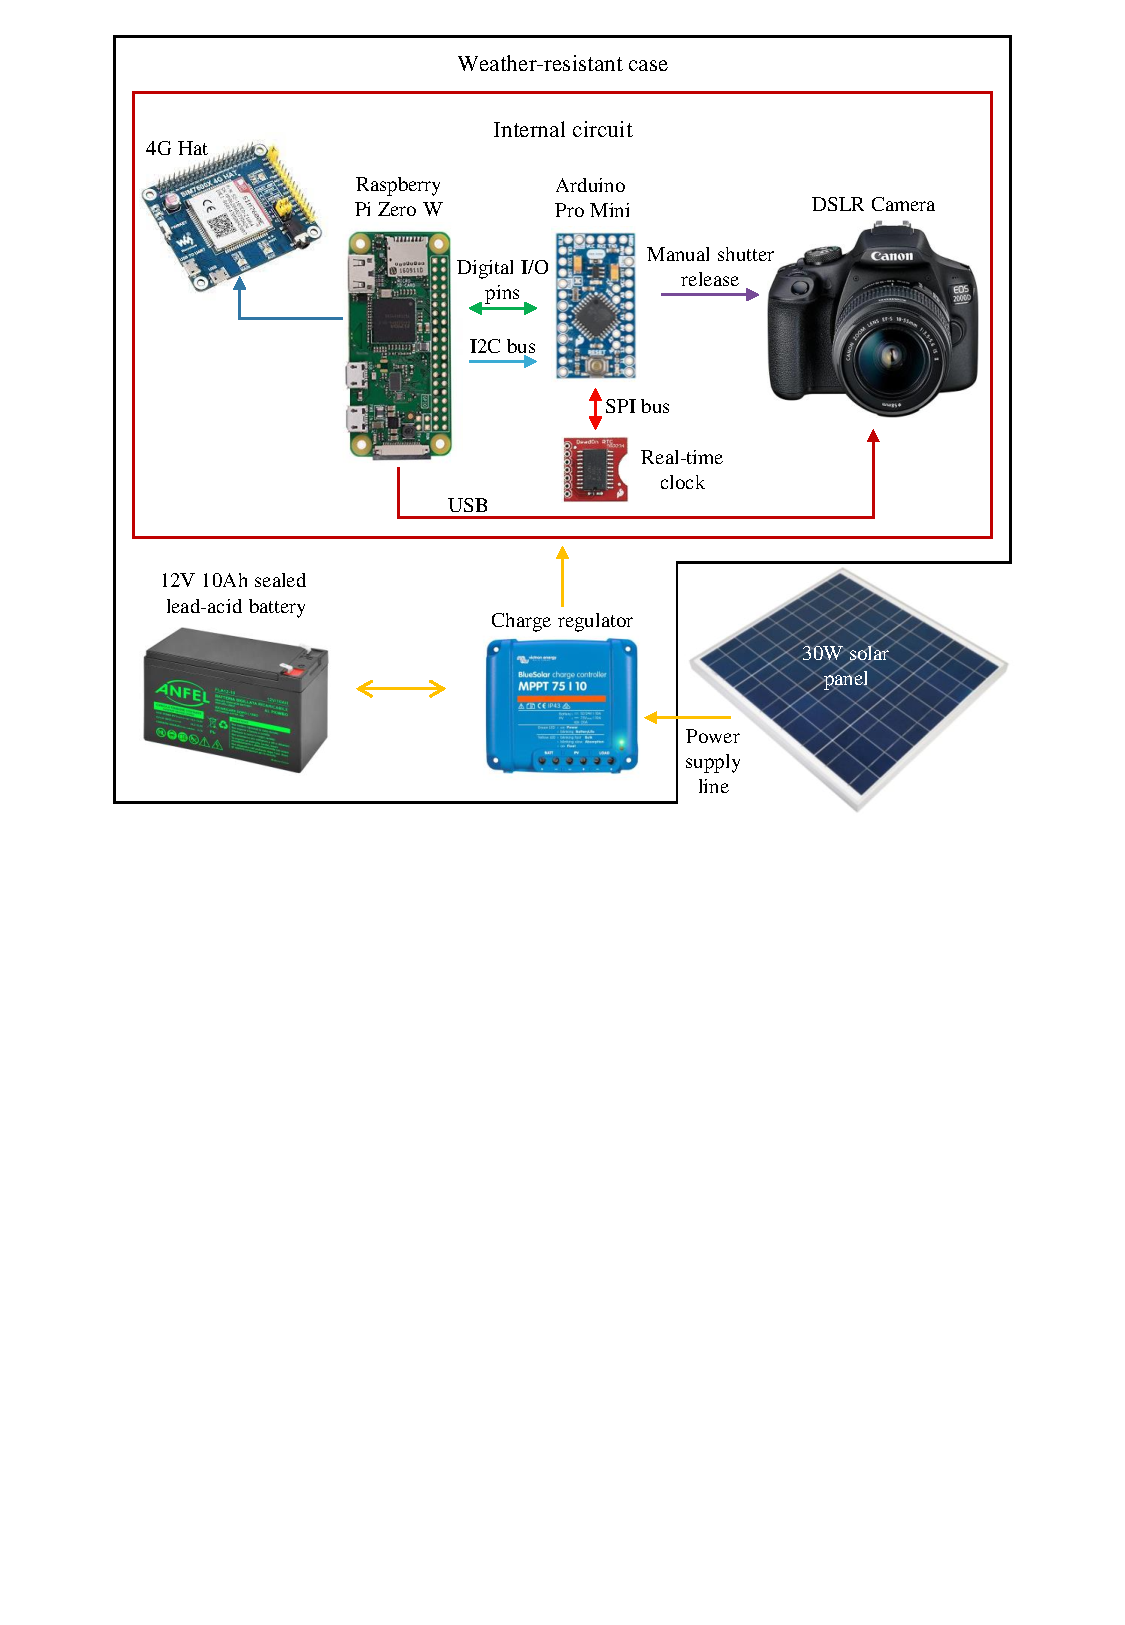
\includegraphics[width=0.6\textwidth]{schema.pdf}
  \caption{Scheme of the proposed acquisition system configuration for a single
    monitoring station. Arrows indicate the direction of signal initiation. Image adapted
    from Greig Sheridan's repository.}
  \label{fig:4:scheme_foto}
\end{figure}

\subsection{Power supply}\label{Power_supply}
Each monitoring unit has its autonomous power supply line (yellow arrows in Figure
\ref{fig:4:scheme_foto}) provided by a solar panel combined with a sealed lead-acid
battery. An MPPT (Maximum Power Point Tracker) charge regulator directly connects with
the unit's internal circuit, providing a regular current supply to the battery
and the load and exploiting all the power generated by the panel. This regulator prevents
any excess current that may damage the connected device, thus increasing the reliability
of the system. Its battery life-saving algorithm modulates the load disconnection level
so that a nearly 100\% recharge is achieved about once every week and, in case of battery
discharging, the whole system is switched off until 100\% recharge of the battery is
achieved.
The whole monitoring system is designed to minimise power consumption, e.g., by powering
off devices responsible for the highest power consumption when not needed.
An estimation of the system's energy consumption guided the choice of the components of
the power supply line. Specifically, the battery and the associated panel must be
accurately dimensioned for the system's purpose. To this end, the Photovoltaic
Geographical Information System (PVGIS) \citep{pvgis}, a tool provided by the European
Commission, was used. PVGIS can estimate the performance of off-grid photovoltaic systems
according to the installation site and it is supported by a database and algorithms for
calculating solar radiation. Tuning the parameters for the Belvedere Glacier location and
the system consumption, we ended up with the specifications of solar panel power of 30 W
and battery voltage of 12 V and capacity of 10 Ah. Some compromises were made, accepting
that the system would not be sufficiently powered in the months with lowest solar
radiation (November, December, January, and February). {\color{red} further details on
    PVGIS simulations for the Belvedere Glacier case study re given.}

\subsection{System control and scheduling}\label{Control}

\begin{figure}[ht!]
  \centering
  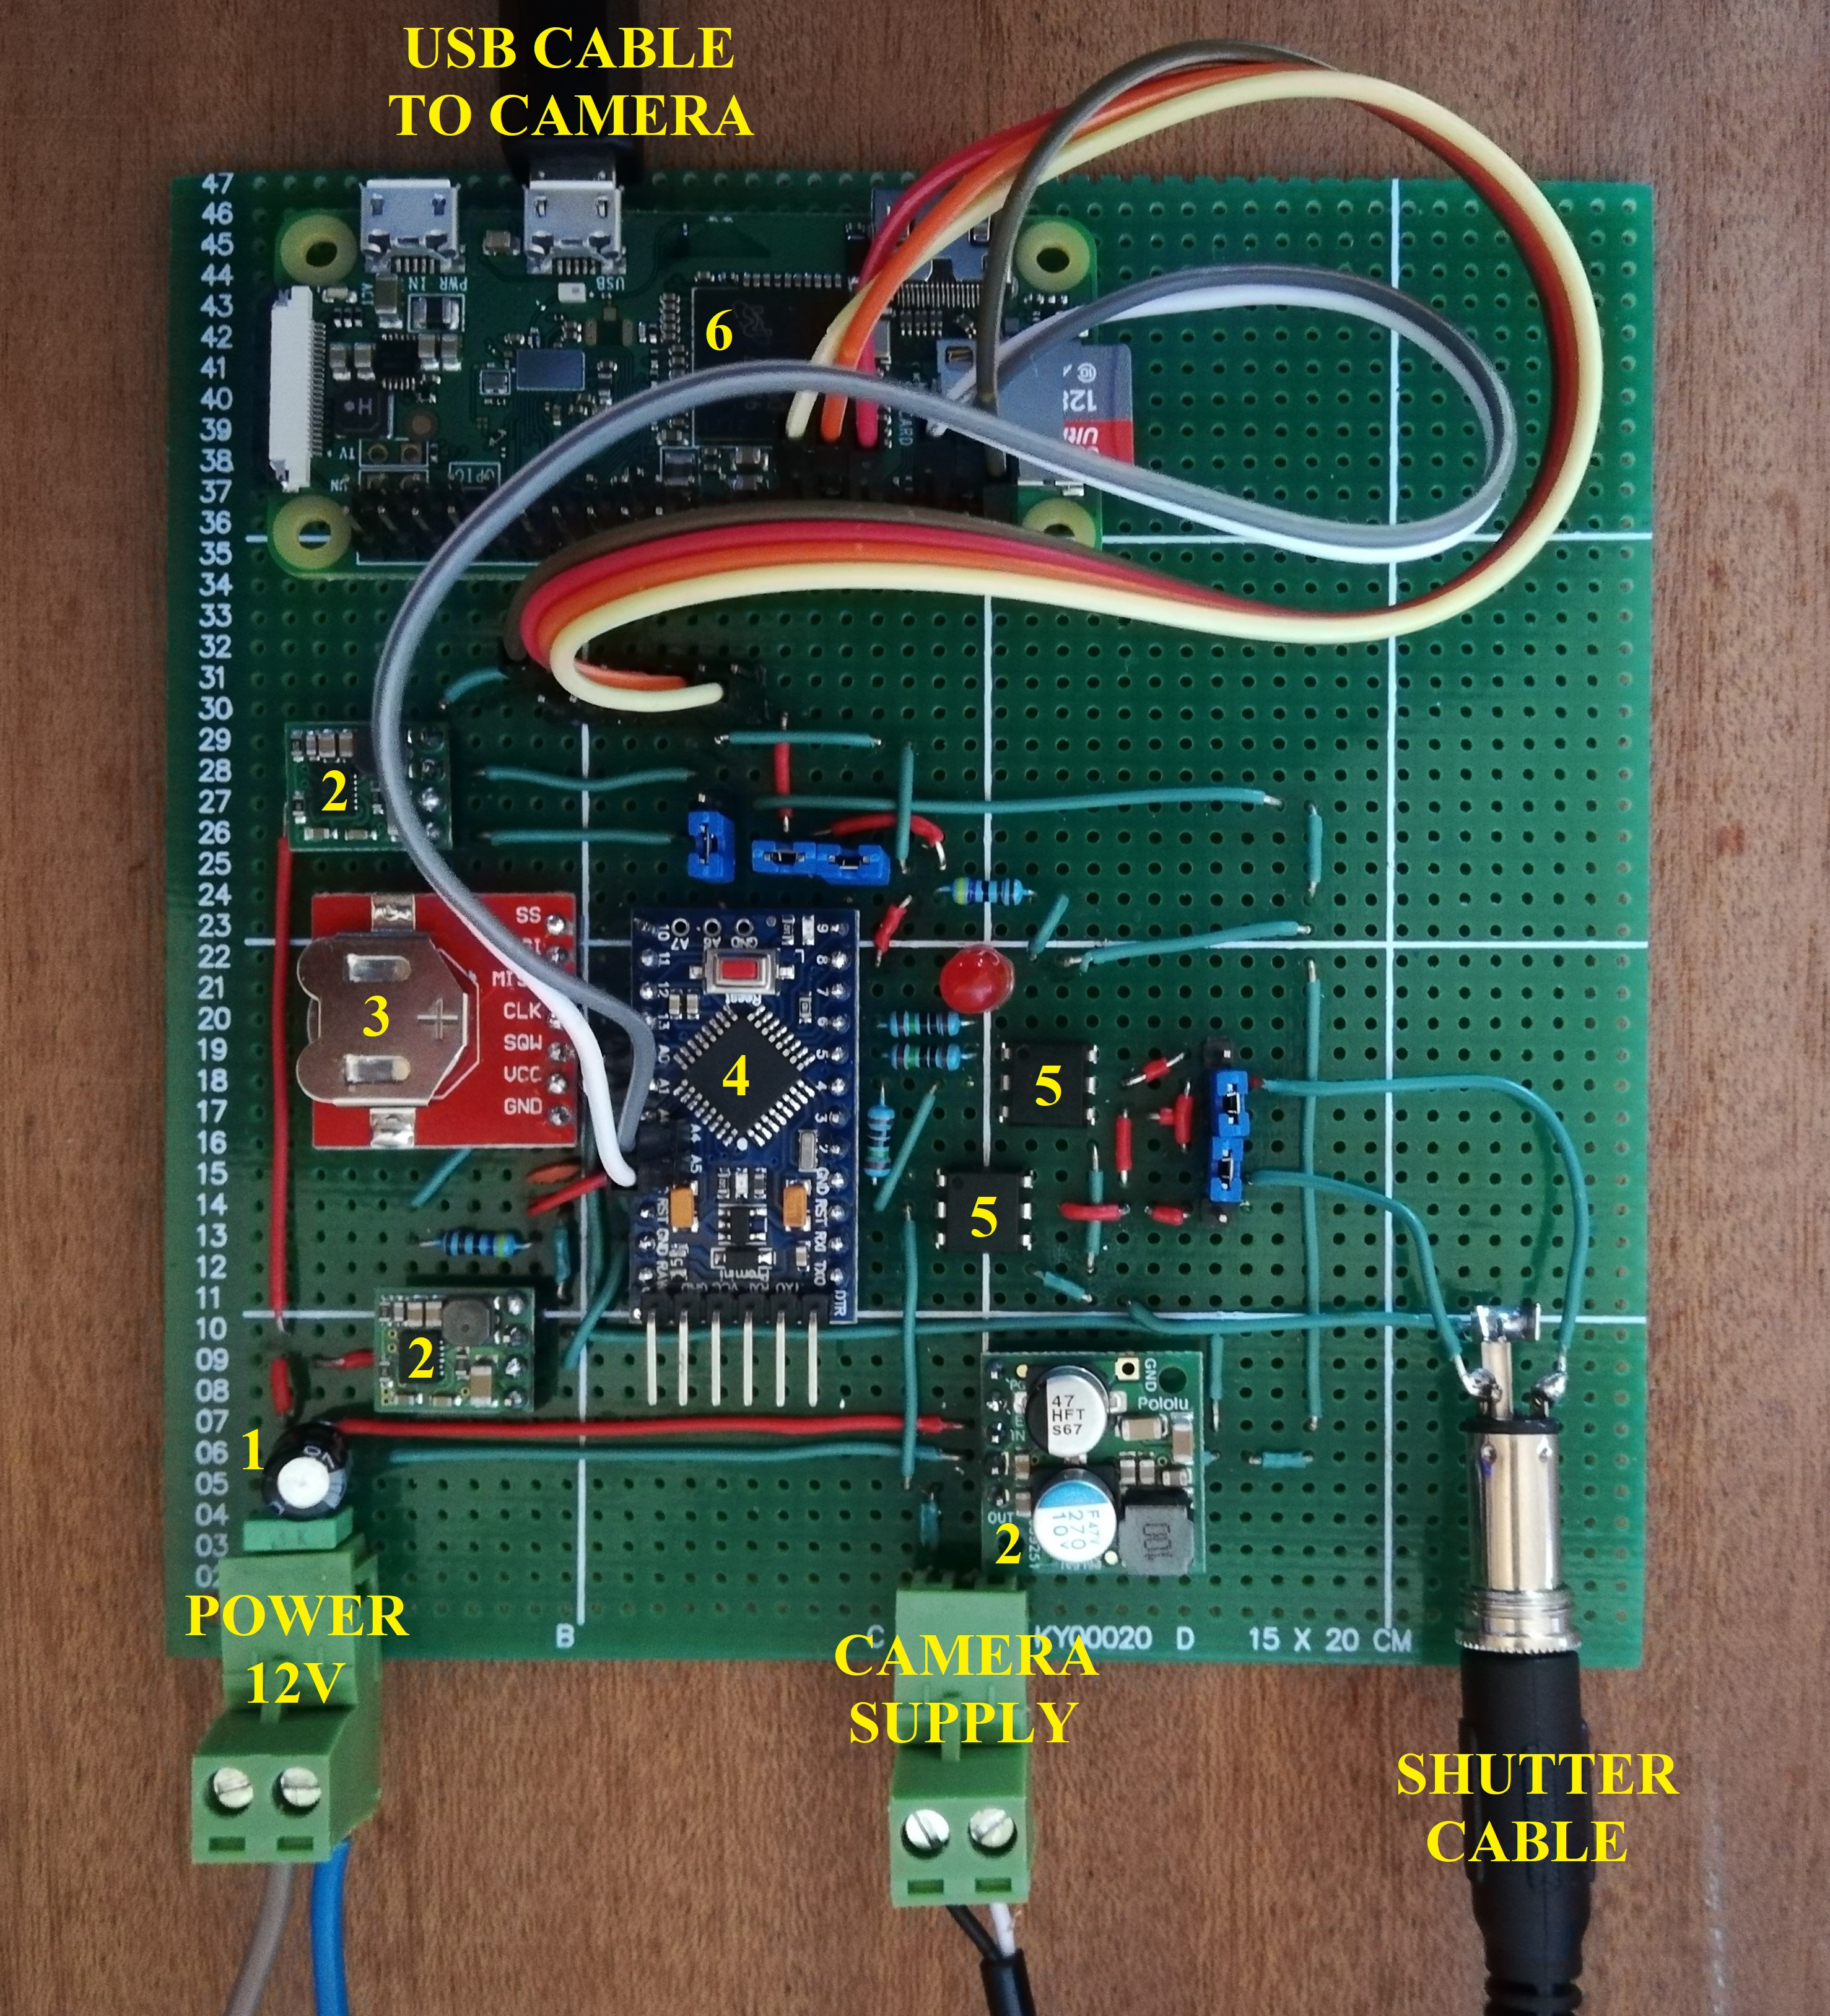
\includegraphics[width=0.6\textwidth]{board.jpg}
  \caption{Stripboard on which are soldered the main components of the internal
    circuit: capacitors (1), voltage regulators (2), real-time clock with coin-cell
    battery (3), Arduino Pro Mini (4), optoisolators (5), and Raspberry Pi Zero W (6).
      {\color{red} Add pic of new board}}
  \label{fig:4:circuit}
\end{figure}

The internal electronic circuit (red box in \figref{fig:4:scheme_foto}) of the
monitoring unit is the only load connected to the power supply and is responsible for all
the system's control and scheduling functionalities.
Its components are a real-time clock (number 3 in \figref{fig:4:circuit}) with a 12
mm
coin-cell backup battery, an Arduino microcontroller (Pro  Mini 328 3.3V 8MHz, number 4
in \figref{fig:4:circuit}), a Raspberry Pi Zero W with 128 GB SD memory card (number
6
in \figref{fig:4:circuit}), and minor elements for connections, isolation (capacitors
and optoisolators numbers 1 and 5 in \figref{fig:4:circuit}), and voltage regulations
(numbers 2 in \figref{fig:4:circuit}).
The circuit was realized manually by soldering wires and components on a stripboard (see
\figref{fig:4:circuit}).

The Arduino communicates through an SPI (Serial Peripheral Interface) bus with an
accurate real-time clock to schedule its actions: waking the camera, firing the shutter
to take a photo, and turning on/off the Raspberry. The Raspberry is able to access the
camera images and transfer them to a remote server via internet connectivity. A large
storage memory is added to the unit to save photos before remote transferring. The
Raspberry also provides a web-based, user-friendly interface
(\figref{fig:4:web-interface}) to configure and monitor the system remotely
\citep{greig}.
An I2C (Inter Integrated Circuit) bus and digital pin connections enable higher-level
communication between these two boards. Among the minor components, we mention the role
of the three voltage regulators. They allow each unit to be powered at the appropriate
voltage and current: starting from the 12 V in input, one delivers 3.3 V and 500 mA to
the Arduino, one 5 V and 2.5 A to the Raspberry and its hat, and the other 7.5 V and 2.4
A to the camera. The Arduino controls the 5V regulator of the Raspberry to reduce
quiescent power consumption when the Raspberry board is off.

Acquisition of a defined number of images, camera triggering and timing, and sending of
images to a remote server can be scheduled thanks to adequate programming of a cyclic
executive program in C++ for Arduino and  of services executing automatically Python
scripts for the Raspberry.
All the monitoring station activities can be remotely scheduled from the terminal or a
user-friendly web interface \citep{greig}. This useful feature allows one to change the
settings and check the behaviour of the system, avoiding the need for manual
intervention. The Raspberry uses the gPhoto2, a Python-based protocol developed to
specifically interact with popular cameras’ firmware, to communicate with the camera and
access the new photos. The  web-based interface service is based on NGINX and Gunicorn,
open-source software for web servers. The interface (\figref{fig:4:web-interface})
consists of a web page accessible with credentials and provides a summary of the system
state and the exact time of the last operations (time of the last shot and the last
upload of images), temperatures of the components, previews of the last images, buttons
to wake up the camera, take a preview photo and schedule the system routine (time and
number of photo acquisition, wake-up time of the Raspberry) and some camera settings.

\begin{figure}[h!]
  \centering
  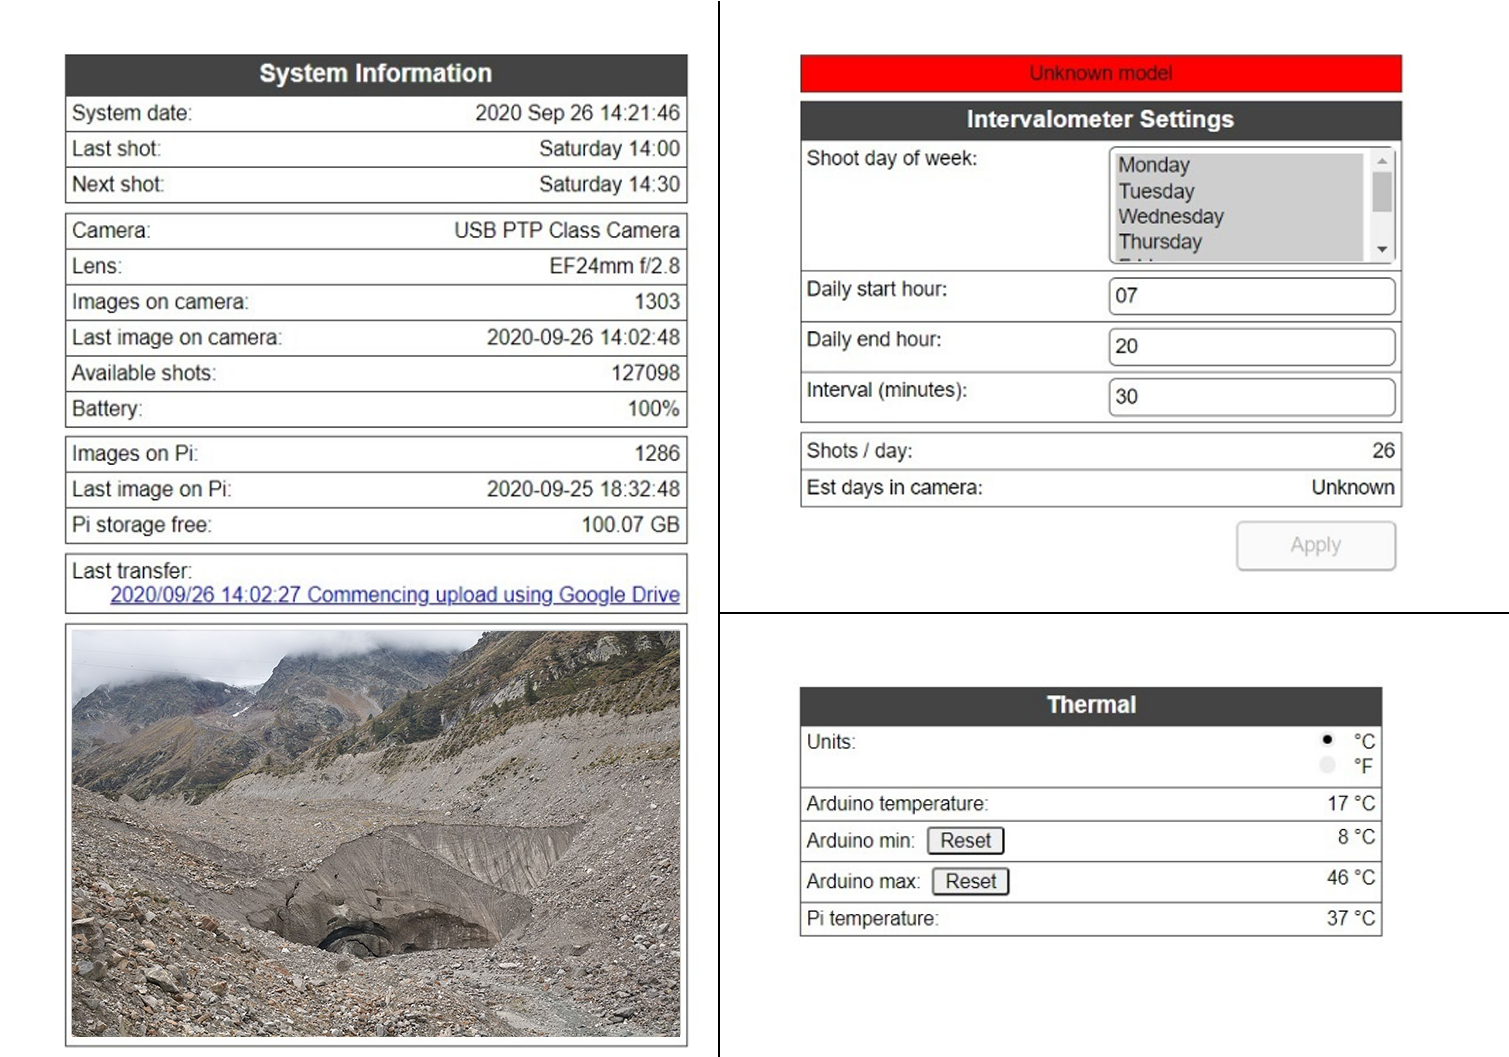
\includegraphics[width=0.8\textwidth]{web_interface.png}
  \caption{Example of some of the pages of the web-based interface to remotely control
    the monitoring units.}
  \label{fig:4:web-interface}
\end{figure}

All the components were chosen because of their low power consumption and their
inter-compatibility. The circuit is robust against power losses due to battery
discharging and is able to auto-recover when power is regained. A low energy consumption
policy is also followed in selecting the scheduling. The camera is switched on only
during the data capture activity. The Raspberry is switched on only once per day when the
connection with the remote server and image transfer is scheduled.

\subsection{Connectivity}\label{Connectivity}
Internet connectivity is crucial to transfer images and to control the units remotely. To
this end, the Raspberry is equipped with the SIM7600E-H 4G hat by Waveshare. The module
supports 4G/3G/2G communication via a SIM card. Raspberry and hat operations are the most
expensive in terms of power consumption. For this reason, the board is switched on only
once a day for a limited period of time, which is kept adequately low to be sustainable
for the system power supply but still sufficient for transferring new images to the
server. We adopted IoT (Internet of Things) SIM cards provided by the multi-operator
service Emnify \citep{emnify}, as it offers the ability to connect to the best-quality
cellular network available and includes flexible and customizable data plans.
Remote access to the devices is allowed by a VPN (Virtual Private Network).
The service costs \texteuro33 per month for a data plan with 6 GB.

\subsection{Case and protection}\label{Case and protection}
The majority of the components need to be protected. Therefore, a solid and compact case
that allows keeping all the parts (with the exception of the solar panel) in the same
location is desirable for the functioning of the system and for convenient
transportation, installation and maintenance. The case should also satisfy the thermal
insulation requirements according to each component's working temperature range. The case
should also be waterproof and robust against different and harsh weather conditions but,
at the same time, provide access for connecting the solar panel and taking pictures. Our
choice was an HPRC 2250 lightweight, waterproof resin case with internal insulating foam.
The foam was found to be useful in enhancing the temperature seal and stabilising the
location of some components, preventing unwanted movements. Holes were drilled in the
case: one sealed with a UV filter of 82 mm to allow the camera to take shots, two others
to give access to the solar panel wires, and others to fix the system to a tripod. The
internal case dimensions (236x182x155 mm) posed a significant challenge in accommodating
all the components inside. In particular, the camera lens dimensions were constrained by
space availability.

\subsection{General performances}\label{General_performances}
The system was subject to several tests before being used in its final application at the
Belvedere glacier site. During these tests, the system proved to be autonomous, robust to
sudden shutdowns, cold-resistant, water-resistant and self-sufficient for a prolonged
period of time with no direct sunlight on the solar panels. Specifically, in the absence
of sunlight, the battery is able to power the system for about nine days before it is
completely discharged. Battery voltage and temperatures of components were monitored,
simulating the absence of solar radiation and low environmental temperatures. See Figure
\ref{fig:4:nominal_performance} for the performances of the system during these tests.
\begin{figure}[h!]
  \centering
  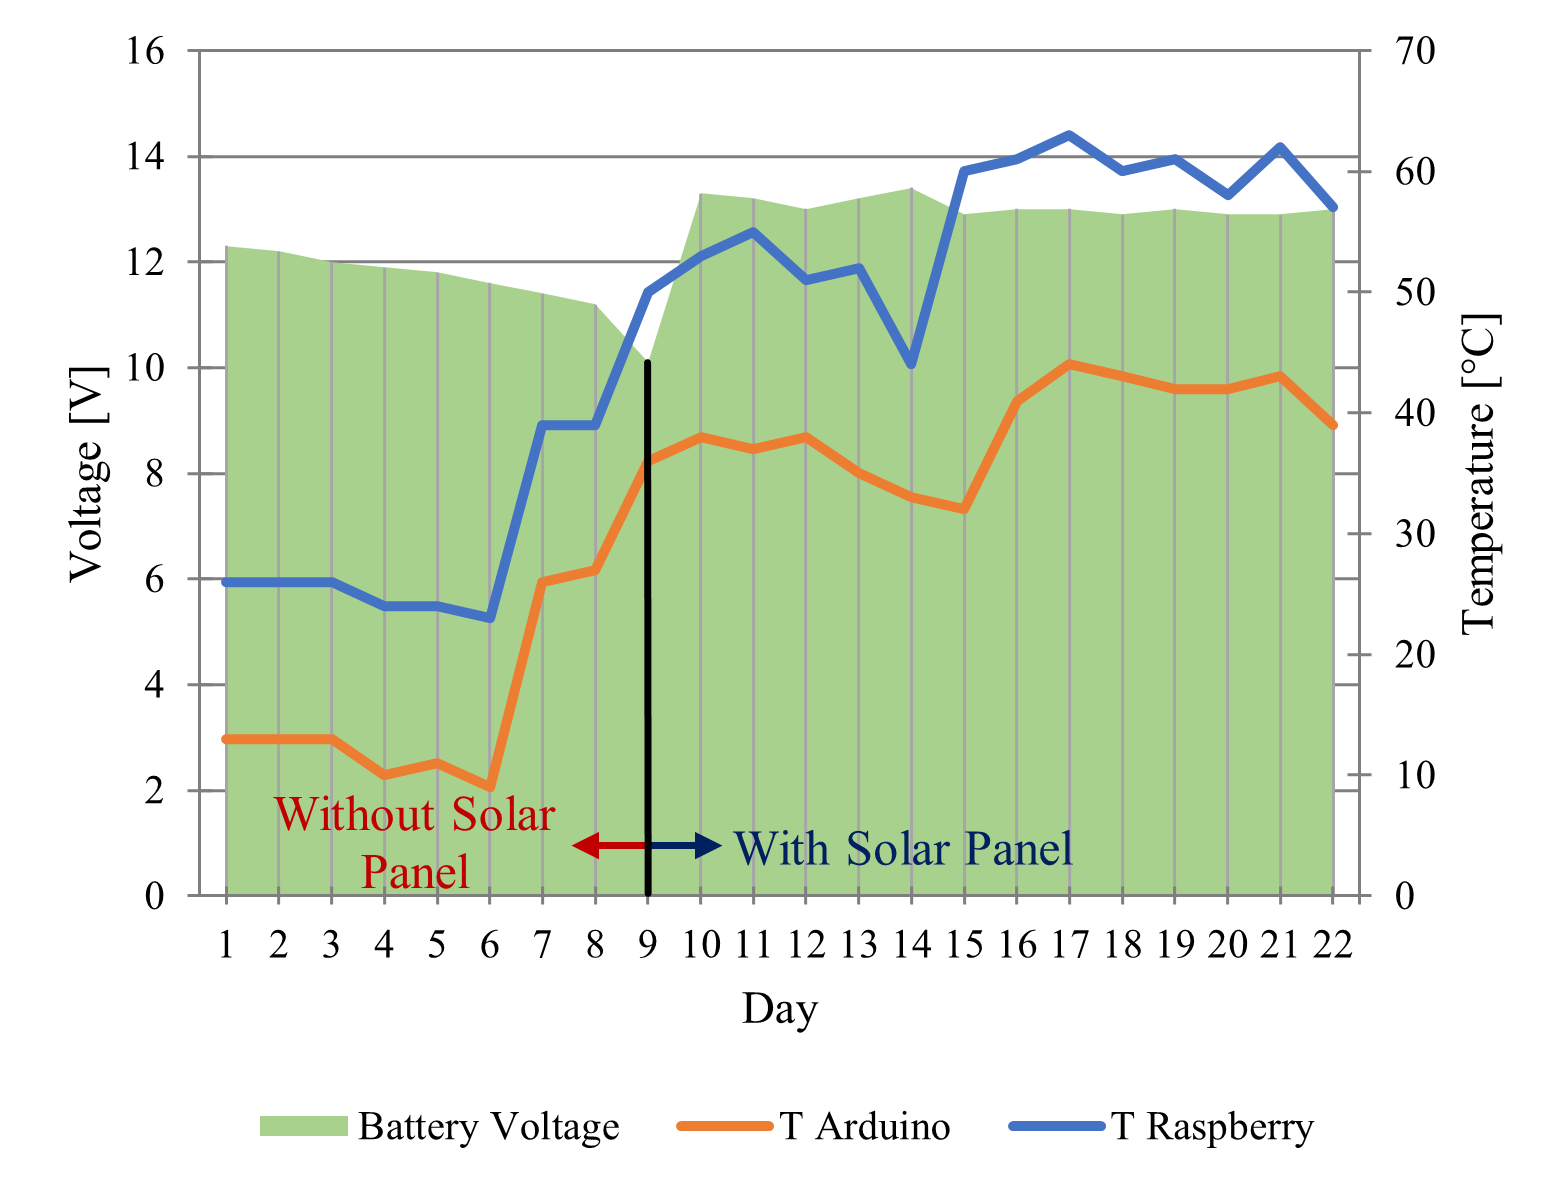
\includegraphics[width=.5\textwidth]{nominal.png}
  \caption{Battery voltage and temperature of boards with and without the solar panel
    during a period of tests. Starting from a fully charged condition, the system was
    kept without solar panel at around 2 °C for the first six days. After nine days, the
    battery was fully discharged and the system was reconnected to the panel and exposed
    to solar radiation.}
  \label{fig:4:nominal_performance}
\end{figure}

\subsection{Camera and lenses}\label{camera_lenses}
The choice of the DSLR camera and of the optics can be considered application-dependent.
Therefore specifications regarding these components are reported in reference to the
Belvedere glacier case study. Each monitoring station was equipped with a DSLR camera
Canon EOS 2000D, with 24.1 MP CMOS \mbox{APS-C} sensor. This model was chosen because of
the limited costs, the high image resolution and its compactness, as it must fit inside
the case. Additionally, another fundamental requirement was camera compatibility with the
gPhoto2 software. In the installation inside the system case, the traditional
rechargeable battery was replaced by a special battery (”fake battery”) equipped with a
power supply cable, which provides a voltage of 7.5 V from the circuit. The camera is
attached to a sliding plate able to vary, with a limited range, and then fix the position
of the camera on the longitudinal axis. Screws fix the camera to the plate and the plate
to the case.

The two stations were installed respectively at $\sim$180 m and $\sim$340 m distance to
the glacier terminus (see \figref{fig:4:studyarea}), avoiding the steep moraines
of the glacier, often prone to collapses and landslides. Therefore, a wide baseline of
$\sim$260 m occurs between the two sensors.
The final positioning of the two cameras was decisive in the choice of optics.
In fact, to ensure comparable Ground Sample Distance (GSD) of the images ($\sim$3 cm
px$^{-1}$), lenses with different focal lengths were employed.
In particular, a Canon EF 24 mm f/2.8 IS USM and a Canon EF 35 mm f/2 IS USM were used
respectively for Camera 1 (stream-wise right) and Camera 2 (stream-wise left).

\subsection{Camera installation}\label{Monumentation}

Monumentation of the two cameras at the Belvedere Glacier site was achieved by choosing
two large stable rocks along the moraines.
Each camera is supported by an aluminium topographic tripod system anchored with steel
dowels and cables to the rocks (\figref{fig:4:final_installation}b).
A central steel tie rod keeps the system in a fixed position.
The choice of an agile monumentation was aimed at having a system that can be rather
easily assembled on site (and also disassembled, if needed), also in a harsh environment,
with limited costs and time.
To install the cameras, in fact, all the equipment was carried in backpacks along the
moraines, sometimes without a marked walking path (e.g., in the case of the stream-wise
left camera).
As a drawback, the analysis of the acquired photos revealed a non-optimal stabilization
of the two cameras.
In fact, small rotations, especially around the vertical axis, and vibrations, mostly
induced by the wind, were experienced.
Though, a perfectly stable monumentation in a mountain environment is hardly achievable.
Therefore, it is not possible to assume the camera orientation as stable a priori, but
camera orientation must be estimated based on some Ground Control Points (GCPs) located
on the ground in stable areas.

It is worth mentioning the performances of the system in terms of costs: our  monitoring
system can be fully reproduced with an average cost of \texteuro2000 per station
(November 2023), including camera (\texteuro400), lens (\texteuro500) and material for
the on-site installation (\texteuro150).
In comparison, commercial time-lapse cameras are expensive
(e.g., PhotoSentinel\footnote{PhotoSentinel: \url{https://photosentinel.com/} (accessed
  on 15/11/23)} cameras cost more than \$5,000.00) and hardly customizable.
The final prototype of the monitoring station is shown in Figure
\ref{fig:4:final_installation}.

\begin{figure}[h!]
  \centering
  \includegraphics[width=.2\columnwidth]{finale1.pdf}
  \includegraphics[width=0.3\columnwidth]{centralina.jpg} \\
  \centering{(a)\hspace{30mm}(b)}\\ \vspace{1mm}
  \caption{(a) Picture of the monitoring unit prototype installed for tests at the
    Belvedere Glacier site. (b) Picture of the final monumentation of the camera
    installed on
    the stream-wise right moraine. {\color{red} TODO: change picture with the final
        installation}}
  \label{fig:4:final_installation}
\end{figure}

\section{Datasets}\label{sec:4:datasets}

\subsection{stereoscopic image sequences}\label{sec:4:stereo}

During the snow-free study period (from 1/05/2022 to 13/11/2022), both camera C1 and
camera C2 were able to acquire images every day, for a total of 197 images. However, 39
images were discarded due to bad weather conditions, such as rain, low clouds, or fog,
resulting in 158 days with valid data for stereo and monoscopic processing

  {\color{red} TODO: write about the images sequence 2022 and 2023}

\subsection{UAV surveys}\label{sec:4:uavsurveys}

Two UAV flights, spaced by a 10-days interval, were conducted in summer 2022 to acquire
ground truth data for assessing the proposed methodology.
The first UAV flight, labelled as UAV-A, was carried out on 28/07/2022 with a DJI
Matrice 300 RTK quadcopter and a DJI Zenmuse P1 camera with a 35 mm lens.
During the survey, 436 images were captured, encompassing both nadiral and oblique
perspectives.
Additionally, 19 Ground Control Points (GCPs) were measured using a combination of a
total station and Differential GPS (DGPS), employing a topographic-grade
GNSS receiver.
The GCPs included both artificial targets and natural features.
During the flight, the UAV was equipped with an on-board RTK GNSS receiver, enabling the
acquisition of camera projection centers with decimetric accuracy.
The photogrammetric block (\figref{fig:4:uavblocks}a) was processed with the commercial
software package Agisoft Metashape \citep{agisoft} by using 14 GCPs and 5 Check Points
(CPs) to evaluate the block accuracy.
The global RMSE evaluated on the CPs was equal to 4.0 cm.

The secondo UAV flight, UAV-B, was carried out on 05/08/2022 with a DJI Phantom
4 RTK, focusing on a smaller portion of the northern lobe of the Belvedere Glacier.
However, due to technical constraints, \textit{moving} GCPs located inside the
glacier body were not measured again.
Therefore, only the fixed targets located outside the glacier were employed.
Among these, 8 targets were designated as GCPs, while the remaining 4 were used as CPs.
The photogrammetric block encompassed 428 nadiral and oblique images, which
were processed using Agisoft Metashape (\figref{fig:4:uavblocks}b).
A global RMSE of 7.5 cm was obtained on the 4 CPs.

\begin{figure}
  \centering
  \subcaptionbox{\label{fig:4:uavblocks:A}}{
    \includegraphics[width=.45\textwidth]{2_UAV-A_280722.png}
  }
  \subcaptionbox{\label{fig:4:uavblocks:B}}{
    \includegraphics[width=.45\textwidth]{2_UAV-B_050822.png}
  }
  \caption{(a) UAV-A block and (b) UAV-B block processed with Agisoft Metashape. The
    flags represent the targets used either as GCPs in the BA or as CPs to evaluate the
    quality of the photogrammetric block.}
  \label{fig:4:uavblocks}
\end{figure}

\subsection{Meteorological monitoring station}\label{sec:4:meteostation}

To analyze the correlation between the Belvedere Glacier dynamics and
external environmental variables, data measured from an Automatic Weather Station (AWS)
located close to the Zamboni Zappa Hut were used.
The AWS is located at an altitude of \SI{2075}{\masl} and at a distance of
2 km from the area of study.
In our study, we analyzed mean daily values of air temperature, precipitation and
incoming solar radiation from 01/05/22 to 15/11/22.

\section{Methodology}\label{sec:4:methodology}
This chapter outlines the methodology developed to monitor the evolution of the Belvedere
Glacier northern lobe.
The daily images were processed using a framework consisting of two parallel processing
chains (\figref{fig:4:workflow}):
(i) a photogrammetric-based stereoscopic approach;
(ii) a DIC-based monoscopic approach.
The daily stereo pairs were used to generate 3D models of the glacier terminus,
enabling the estimation of ice volume loss on a daily basis by computing point cloud
differences along the main flow direction.
However, due to limited overlapping views of the two cameras, the stereoscopic approach
primarily provides a 3D reconstruction of the terminal ice cliff (dashed-blue area in
\figref{fig:4:studyarea}b).
Consequently, deriving the 3D surface velocity field of the glacier solely from
photogrammetry was not feasible.
The image sequence captured by camera C2, offering a higher viewpoint and broader
coverage of the glacier surface, was employed to determine the glacier's surface velocity
over a larger area of the north lobe of the Belvedere Glacier (dashed-green area in
\figref{fig:4:studyarea}b).

\begin{figure*}[ht]
  \centering
  \includegraphics[width=154mm]{3_general_workflow.png}
  \caption{General workflow with two parallel processing chains involving stereoscopic
    reconstruction of terminal ice cliff from stereo-pairs of images to derive ice volume
    losses at the glacier terminus and glacier retreat and monoscopic digital-image
    correlation to derive surface velocities.}
  \label{fig:4:workflow}
\end{figure*}

\subsection{Image selection}\label{sec:4:imageselection}

Once the acquired images have been received from the monitoring system, an
automatic selection of the images was performed to exclude the ones acquired in rainy,
foggy, or poor lighting conditions.
This selection was based on the analysis of images median
entropy~\citep{tsai2008entropy}:
the images with a low value over the entire image were rejected.
Additionally, a visual inspection was performed on the entire image dataset.
The inspection had the following objectives:
(i) selecting only one image per day;
(ii) rejecting poor quality images that were not automatically rejected,
and images in which the fixed targets placed along the moraines were not visible;
(iii) detecting of sudden changes in the morphology of the glacier
terminus (e.g., icefall).

\subsection{Camera calibration}\label{sec:4:cameracalibration}

Each camera was mounted with all its electronics inside a waterproof case and protected
by a neutral filter that was glued to the case and fixed in front of the cameras.
Since the filter introduced additional distortion, the cameras need to be calibrated
inside the boxes to reproduce the final setup.
Therefore, a two-step approach was taken: first, a 120 cm x 70 cm calibration board with
a checkerboard printed on it was used to estimate an initial set of parameters for the
interior orientation \citep{zhang_flexible_2000}.
To this end, the cameras were mounted on tripods inside their cases while the calibration
board was moved and rotated in front of the camera to simulate a convergent hemispheric
acquisition.
For each camera, about 30 images were collected and processed in Agisoft Metashape to
obtain a first estimate of the interior orientation.
However, the average camera-to-panel distance was much smaller than the actual
camera-to-glacier distance.
Therefore, a refinement of the calibration was performed in-situ by incorporating the
stereo pair acquired by the cameras on 28/07/22, within the UAV-A block, carried out on
the same day.
This block was processed with Agisoft Metashape to refine the interior camera
orientation of the stereo cameras, aided by the increased robustness of the block given
by the additional matches between the two images taken by camera C1 and C2 and the UAV.

An additional challenge was represented by camera interior orientation stability over
time.
From experimental evidence, the interior orientation parameter that suffered the most
because of temperature variations that occurred in mountain environment
was the camera principal distance \citep{Elias2020}, while the other parameters
remained more stable during time.
To mitigate the impact of temperature-induced variations, it was crucial to incorporate
camera self-calibration during the stereoscopic processing at each epoch to refine the
pre-calibrated principal distance.

\subsection{Camera stability and GCPs}\label{sec:4:stability}

Since the two cameras were mounted on topographic tripods, the stability of the cameras
was not perfectly guaranteed. In particular, the two cameras experienced small vibrations
around their pivots due to wind gusts.
On the other hand, the position of the cameras was constrained by topographic heads that
kept the position of the camera center constant to the centimeter level.
Therefore, the baseline of the cameras can be reasonably considered as constant, with a
value of \SI{261.55}{\meter}.
On the other hand, camera angular vibrations implied that the relative orientation of the
cameras must be estimated at each epoch.
Moreover, to fix the world reference system over time, absolute orientation of the
stereo model was required.
To this end, the position of the cameras was measured in-situ using a topography-grade
GNSS receiver in RTK.
In addition, four GCPs were materialized with plastic targets, anchored to stable rocks
in front of the terminal ice cliff and along the streamwise left
moraine (\figref{fig:4:studyarea}a).
While the minimum requirement to estimate a Helmert transformation would have been just
the two cameras' location and one one GCP, having a redundant number of GCPs overcomes
the
possibility that on some days not all GCPs were clearly visible in the images due to low
clouds or fog.
Additionally, GCPs can be included into the BA to refine the cameras' interior
orientation,
and in particular the camera's focal length.

As the cameras are subjected to slight rotations, the image coordinates of the GCPs'
projections must be detected at each epoch.
To this end, a feature tracking routine was developed based on the ImGRAFT TemplateMatch
method~\citep{Messerli2015}, enabling the detection of a template defined on a reference
image within a target image through DIC.
The routine utilized the orientation correlation algorithm~\citep{fitch2002_OC},
providing increased
robustness against illumination changes and achieving sub-pixel accuracy
\citep{Dematteis2021,Heid2012_evaluation_xcorr}.

\subsection{Stereoscopic image processing workflow}\label{sec:stereoworkflow}

\begin{figure}
  \centering
  \includegraphics[width=.5\textwidth]{3_stereo-workflow.png}
  \caption{Scheme of the stereoscopic workflow performed with ICEpy4D. At a generic epoch
    \(i\), new features are extracted and matched.
    At the same time, features from the previous epoch \(i-1\) are tracked on the current
    epoch images. After geometric verification, features successfully
    matched are used for 3D scene reconstruction. Point clouds obtained on
    different days are used to compute ice volume differences and glacier
    retreat.}
  \label{fig:4:stereo-workflow}
\end{figure}

% References
% \bibliography{references}
% \addcontentsline{toc}{section}{References}
% \bibliographystyle{apacite}

\graphicspath{{figures/chapter5/}}
\onehalfspacing

\chapter{Towards a low-cost multi-camera multi-epoch monitoring with deep learning photogrammetry}\label{ch:5}

\vfill

\newthought{This chapter is based on:}

\begin{itemize}
  \item Morelli, L., Ioli, F., Maiwald, F., Mazzacca, G., Menna, F., and Remondino, F. (2024). DEEP-IMAGE-MATCHING: A TOOLBOX FOR MULTIVIEW IMAGE MATCHING OF COMPLEX SCENARIOS, Int. Arch. Photogramm. Remote Sens. Spatial Inf. Sci., XLVIII-2/W4-2024, 309–316, \url{https://doi.org/10.5194/isprs-archives-XLVIII-2-W4-2024-309-2024}. 
\end{itemize}

\newpage

\section{Introduction}\label{sec:5:intro}

% \begin{itemize}
%     \item Why it is important to implement a multi-camera system
%     \item Which are the challenges and the advantages
%     \item Motivate Deep-Image-Matching because no existing library allows for multi-view matching with DL features for complex scenarios
%     \item Showcase a few case studies with DIM in complex scenarios and test case with UAV images on belvedere (simulate third camera)
% \end{itemize}

\chref{ch:4} demonstrated the potential of a low-cost stereoscopic camera system for short-term monitoring of glacier dynamics. 
However, the usage of a stereo camera only poses limitations on the viewing area that can be covered by the system, especially under sub-optimal viewing conditions and acquisition geometry.
To further enhance our 3D reconstruction capabilities, this chapter aims to introduce a transition to a multi-camera approach.  
A multi-view framework offers several compelling advantages for glaciological studies.  
Firstly, overlapping fields of view from multiple cameras reduce occlusions, ensuring better coverage of complex glacier surfaces. 
Secondly, multiple image perspectives refine 3D reconstructions, providing greater accuracy and reducing uncertainties. 
Finally, a multi-camera system lends itself to expansion, allowing the integration of additional cameras over time for long-term monitoring and evolving research needs.

As discussed in \chref{ch:4}, wide camera baselines, strong viewpoint changes, and the often low-texture surfaces inherent to glacial environments pose significant hurdles for traditional feature-matching techniques.
Therefore, standard SfM software packages are often not suitable for performing photogrammetric reconstruction in challenging scenarios.
This complexity introduces the need for cutting-edge approaches, such as the Deep-Image-Matching (DIM) toolbox presented in this chapter.
DIM is a versatile toolbox designed for both traditional and DL-based multi-view image matching. 
It addresses a crucial gap in existing libraries: the lack of tools specifically tailored for multi-view matching under challenging conditions by using hand-crafted and DL local features and matching algorithms.

This chapter will explore the potential of DIM by testing it against challenging scenarios (wide baselines, viewpoint differences, low texture, and multi-modal images), highlighting its potential advantages over traditional feature-matching methods.  
The goal is to assess the suitability of DL local features for photogrammetric applications, by exploiting the DIM library to streamline their use. 
Unfortunately, a multi-camera monitoring system has not been installed yet at the Belvedere Glacier. 
Therefore, this chapter will focus on the software component and we will simulate a multi-view scenario on the Belvedere Glacier using existing UAV imagery. 

% In comparison to existing literature, this work introduces several innovative aspects: 
% \begin{itemize}
%     \item Examination of DL local features' performance on high-resolution images. 
%     \item  Addressing the challenge of managing rotations within the matching process. 
%     \item Implementation of local refinement techniques to enhance feature matching accuracy. 
%     \item Extension of semi-dense matchers, such as LoFTR and RoMa, to accommodate multi-view scenarios. 
%     \item Evaluation of DL features on photogrammetric datasets to validate their suitability for real-world applications. 
%     \item Introduction of a new evaluation metric, in addition to the conventional Root Mean Square Error (RMSE) assessment on checkpoint data. 
%     \item Presentation of three additional applications showcasing the versatility of DL features (RGB to thermal image matching, ...). 
% \end{itemize}

% \begin{figure}
%     \centering
%     \includegraphics[width=1\textwidth]{local_feats_history}
%     \caption{Timeline development of detectors, descriptors and matchers from preliminary works, hand-crafted, machine-learning, and deep-learning local features. (Cit.)}
%     \label{fig:5:feats_history}
% \end{figure}

\section{Limitation of Deep Learning local features}\label{sec:5:limitation_dl_feats}

As discussed in \secref{sec:4:localfeatures}, in the past few years, a large number of trainable algorithms for robust local feature extraction and matching have been developed \citep{Yao_2021, remondino2022_at_with_dl}.
DL techniques, and particularly attention-based architectures~\citep{vaswani2023attention}, have emerged as a powerful technique for extracting and matching features in difficult conditions, such as wide baselines and significant radiometric differences~\citep{jin_image_2021, Yao_2021}.

Although DL local features offer several advantages, their limited rotational invariance remains a constraint, particularly when analyzing images with diverse orientations. 
While some initial studies highlighted this issue, many subsequent approaches have not prioritized solutions. 
This may stem from the common use of datasets with minimal rotational variability (e.g., upright images) within the computer vision community, which are common in aerial and UAV photogrammetric datasets \cite{Bkman2022_se2loftr}. 
Recently, some end-to-end approaches like LIFT \citep{yi2016lift} and LFNet \citep{ono2018lfnet}, and semi-dense methods like RoRD \citep{parihar2022rord} and SE2-LoFTR \citep{Bkman2022_se2loftr}, demonstrate progress in achieving rotational invariance. 
Recent works with Steerable CNNs \citep{cohen2016steerable}, which are examples of group equivariant neural networks that allow for \textit{steering} the descriptors to make them invariant by the rotation, further address this limitation \cite{Bkman2022_se2loftr, bokman2023steerers}.
Nevertheless, the number of approaches specifically addressing this problem is minimal compared to the overall interest in DL-based feature-matching algorithms.
On the other hand, the most common approach to address large rotation is still to compensate by iteratively rotating images during matching, but this becomes computationally intensive for large datasets.

Another limitation of DL approaches is their computational expense, which makes them unsuitable for deployment on full-resolution images, which are crucial for leveraging the available radiometric information in high-accuracy photogrammetric applications.
In addition, it's worth noting that training itself often occurs on low-resolution images, a concern highlighted in \cite{Wu2024_evaluation_dlstereo}, whose impact remains uncertain.
Training could have been generalized enough not to require additional training on high-resolution images. 

While the potential of these approaches under extreme lighting conditions and radiometric variations is increasingly evident \textcolor{red}{[Ref]}, some preliminary experiences suggest that these approaches may lack locally accurate identification \textcolor{red}{[Ref]}. 
Indeed, despite the existence of DL approaches for several years, their utilization in photogrammetric applications remains relatively limited. 
\textcolor{red}{[Include relevant papers: satellite image analysis, glacier monitoring, and applications aimed at enhancing augmented reality (AR) and virtual reality (VR) experiences, registering laser scanner point clouds, Precision Agriculture Agriculture (Gao et al., 2024)]}.

\begin{figure}[ht]
    \centering
    \includegraphics[width=1\textwidth]{dim_workflow_simple}
    \caption{Scheme of the DIM workflow.}
    \label{fig:5:dim_workflow}
\end{figure}

\section{Deep-Image-Matching}

% Given a set of unordered images, Deep-Image-Matching can perform the matching operations and return the corresponding points between images. It is developed in Python and publicly available on GitHub (\url{https://github.com/3DOM-FBK/deep-image-matching}), it supports both CLI and GUI as well as a wide range of local features and matching algorithms, spanning from the traditional ones to recent state-of-the-art learning approaches. Available local features include ORB, SIFT, SuperPoint (DeTone et al., 2020), ALIKE (Zhao et al., 2022), ALIKED (Zhao et al., 2023), DISK (Tyszkiewicz et al., 2020), Key.Net (Barroso-Laguna et al., 2019) + HardNet8 (Pultar, 2020), DeDoDe (Edstedt et al., 2023b). SuperGlue (Sarlin et al., 2020), LightGlue (Lindenberger et al., 2023), LoFTR (Sun et al., 2021), SE2-LoFTR (Bökman and Kahl, 2022), and RoMA (Edstedt et al., 2023a) are implemented as matchers. Additionally, KORNIA python library (Riba et al., 2020) can be used for nearest neighbour matching.
% Image pairs to be matched can be chosen by the user (custom pair option), or they can be automatically selected by other strategies, including all possible pairs (brute force), sequential matching (sequential), or image retrieval using global descriptors (retrieval). Image pairs can also be chosen by running a brute force on low-resolution images to limit computational time (option matching lowres).
% For high resolution images (i.e., images with the longest edge larger than 5000 px), feature extraction and matching are carried out by tiling the images on a regular grid to fit into GPU memory, while the selection of the tiles to be matched is guided by a first matching on low-resolution images. Features matched on each image pair are verified by using PyDegensac (Mishkin et al., 2015) to reject outliers. Geometrically verified tie points are then stored in a SQLite3 database to be imported in COLMAP, or in the openMVG format, ready for the bundle adjustment in the respective software. To import the solution in other photogrammetric software (e.g. Metashape), image orientation is performed with pycolmap library, and 3D tie points are exported in the Bundler format (Snavely et al., 2006).

Deep-Image-Matching\footnote{\url{https://github.com/3DOM-FBK/deep-image-matching}} (DIM) is a flexible, open-source Python library designed for robust multi-view image matching, leveraging both hand-crafted and DL matching techniques.  
Given a set of unordered images, DIM can perform the matching operations and return the corresponding points between images, providing the essential foundation for bundle adjustment and accurate photogrammetric reconstruction.

DIM's primary goal is to provide a user-friendly interface to a wide selection of state-of-the-art computer vision algorithms for matching and tracking corresponding points across unordered images.
Additionally, DIM aims to overcome the main limitations of DL-based matching approaches that pose challenges for their practical usage in photogrammetry and remote sensing. 
These limitations include sensitivity to rotation changes, computational bottlenecks with high-resolution images (e.g., larger than 3000 px on the longest edge), difficulties in achieving sub-pixel accuracy, inefficient image pair selection for large datasets, and compatibility issues with existing SfM software packages.  

DIM employs a modular workflow designed for effective multi-view matching \figref{fig:5:dim_workflow}.
DIM itself does not perform the bundle adjustment and scene reconstruction, but it is designed to ensure seamless integration with various popular SfM software packages within the remote sensing and computer vision communities. 
These include COLMAP \citep{schoenberger2016sfm}, OpenMVG \citep{moulon2016openmvg}, MicMac \citep{rupnik2017micmac}, Agisoft Metashape\footnote{\url{https://www.agisoft.com/}}, 
and any other software package that supports the import from a Bundler solution format \citep{Li_Snavely_2018_MegaDepth}.
Additionally, DIM can be easily integrated into a multi-camera multi-epoch pipeline, e.g., by exploiting the multi-temporal functionalities of ICEpy4D (see \chref{ch:4}).

The process begins with a pre-processing stage where users select from different matching strategies (brute-force, low-resolution guided, sequential, image retrieval, or custom) to intelligently select the pair of images for optimized matching. 
Additionally, DIM provides a module for addressing the challenge of rotated images within datasets (e.g., in the case of aerial or UAV surveys) by automatically identifying the ideal rotation angle between image pairs, significantly boosting matching accuracy. Users can opt to match images at their original resolution or employ down-sampling or up-sampling techniques managed by a quality parameter.
To handle high-resolution imagery, DIM offers the added capability of image tiling, ensuring efficient processing without compromising detail. 

For the actual matching, DIM supports various combinations of local feature and matching algorithms, named \textit{pipelines}, optimized for diverse problem domains. This allows users to tailor the workflow to their specific needs. 
Each pipeline consists of two main components: (i) an \textit{extraction} step that is responsible for extracting local features from all images in the dataset; and (ii) a \textit{matching} step that matches the extracted local features across the image pairs selected by the chosen matching strategy.  

DIM supports a wide range of local features and matching algorithms, spanning from the traditional ones to recent state-of-the-art learning approaches. 
Available local features include ORB \citep{Rublee2011}, SIFT \citep{Lowe2004}, SuperPoint \citep{DeTone_2018}, 
ALIKE \citep{zhao2022alike}, ALIKED \citep{zhao2023aliked}, DISK \citep{tyszkiewicz2020disk},
Key.Net \citep{barrosolaguna2019keynet} + HardNet \citep{pultar2020improving}, DeDoDe \citep{edstedt2024dedode}.
DIM implements SuperGlue \citep{sarlin2020superglue}, LightGlue \citep{lindenberger2023lightglue}, and traditional nearest-neighbor algorithms based on the KORNIA library \citep{riba2019kornia} as local features matchers. 
Additionally, the detector-free matchers algorithms LoFTR \citep{sun2021_loftr}, SE2-LoFTR \citep{Bkman2022_se2loftr}, and RoMA \citep{edstedt2023roma} are included in DIM and allows for a semi-dense scene reconstruction.

\subsection{Matching strategies}\label{sec:5:matching_stategies}

\begin{figure}[ht]
  \centering
  \subcaptionbox{Unordered set\label{fig:5:matching_strategy:unordered}}{
    \includegraphics[height=3.5cm]{match_strat_unordered}
  } \qquad
  \subcaptionbox{Bruteforce\label{fig:5:matching_strategy:bruteforce}}{
    \includegraphics[height=4cm]{match_strat_bruteforce}
  }\\ \vspace{2mm}
  \subcaptionbox{Sequential (overlap=2)\label{fig:5:matching_strategy:sequential}}{
    \includegraphics[height=5cm]{match_strat_sequential}
  }\qquad
  \subcaptionbox{Low-res preselection\label{fig:5:matching_strategy:lowres}}{
    \includegraphics[height=5cm]{match_strat_lowres}
  }  
  \caption{Scheme of the main different matching strategies implemented in DIM given an unorered image set (a). (b) Bruteforce strategy (i.e., \textit{all-to-all)}; (c) Sequential strategy with overlap equal to 2 (i.e., match all images with next 3 images, note that the overlap parameter is zero-based); (d) Low-resolution guided matching strategy (i.e., perform a fast bruteforce on low-resolution images and match only good candidates at high resolution).}
  \label{fig:5:matching_strategy}
\end{figure}

The matching strategy defines how the pairs of images to be matched are selected to optimize the matching process. The choice of matching strategy plays a crucial role in optimizing image matching, especially with large datasets.  

DIM offers a versatile range of strategies to address diverse use cases. 
The \texttt{brute-force} approach provides the most comprehensive exploration by attempting to match every image with every other (\figref{fig:5:matching_strategy:bruteforce}). 
This method is computationally intensive but can be valuable for small datasets or complex scenarios where other strategies may yield insufficient matches. 
The image pairs are obtained by computing combinations of n elements in 2 places, where n is the number of images in the dataset. 
Therefore, the computation complexity by $ p = C(n,2) = \frac{n*\left(n-1\right)}{2}$, where $p$ is the number of pairs.

For image sequences acquired in order by a moving camera, (e.g., Visual Odometry or SLAM), the \texttt{sequential} strategy offers optimized efficiency by matching each image with a defined number of subsequent images. 
The overlap parameter defines the number of consecutive images to match sequentially (\figref{fig:5:matching_strategy:sequential}).
The computational complexity is given by $p = \left(n-O\right) * O $, where $O$ is the overlap parameter.

The \texttt{matching\char`_lowres} enhances computational efficiency by initially analyzing downsampled images to pre-filter pairs based on valid matches detected at lower resolution and considered as inliers after a geometric verification (\figref{fig:5:matching_strategy:lowres}). 
By default, the minimum number of valid matches is 20 but it can be tuned by the user. 

The \texttt{retrieval} strategy allows to use of global features to determine the pairs of images that are likely to see the same scene \citep{Yang2013_imageretrieval}. 
Global features encode the full images into a neural network and therefore they are widely used to tackle visual place recognition problems \citep{napoletano2017visual}. 
DIM makes use of hloc \citep{Sarlin_2019_hloc} for extracting and matching global features and it supports NetVLAD \citep{arandjelovic2016netvlad},  openIBL \citep{ge2020selfsupervising}, and CoSpace \citep{Hong_2019} global features.  

Finally, the \texttt{custom\char`_pairs} option grants users precise control over the matching process, allowing the specification of exact image pairs via a text file. 
This enables tailored workflows for specific research objectives. 

\subsection{Image resolution and tiling}\label{sec:5:tiling}

DIM provides extensive control over image resolution before feature extraction and matching, providing flexibility for different user needs and hardware constraints. 
This functionality is particularly important when using DL-based local feature extractors and matchers that rely on GPU parallelization for best performance. 
They face limitations when processing large images on consumer-grade GPUs, which typically have limited memory resources. 
The image size threshold varies depending on the available GPU memory and the specific algorithms used (detector-free matchers tend to be particularly memory-intensive). 
As a general guideline, images with a long edge of up to 3000 pixels can often be processed on a 12GB GPU using a combination such as SuperPoint and LightGlue. 

To address this challenge, DIM offers several resolution management strategies: images can be downsampled by a factor of 2, 4, or 8 (medium, low, or lowest quality settings in DIM) using OpenCV's pixel-area relation (bilinear interpolation). 
This approach may be appropriate when computational efficiency is a priority. Alternatively, for DL features that operate with pixel-level accuracy (e.g., SuperPoint), upsampling by a factor of 2 (DIM's highest quality setting) using bicubic interpolation can improve subpixel detection capabilities.  

To preserve high-resolution detail in large images, DIM supports breaking them into smaller, regular tiles.
This is critical when using end-to-end detector-free matchers (e.g., LOFTR, RoMa), as their combined extraction and matching steps are particularly memory intensive. 
DIM's tiling allows the user to specify tile dimensions or the number of tiles per row/column.
An overlap between neighboring tiles can be specified to avoid having no features extracted along the tile boundaries. 
The software automatically handles zero padding to maintain consistent tile sizes throughout. 

When using image tiling, DIM handles local feature extraction separately, processing each tile sequentially. 
However, tile-based feature matching offers several strategies: \texttt{exhaustive}, \texttt{preselection}, and \texttt{grid} mode.
In \texttt{exhaustive} mode, features from each tile of the first image are matched against features extracted from all tiles of the second image. 
This mirrors the brute-force approach to image pair selection (see \secref{sec:5:matching_stategies}) and ensures comprehensive exploration of potential matches, but can be computationally intensive. 
The \texttt{preselection} mode prioritizes efficiency and is the default approach. 
An initial low-resolution matching step identifies tile pairs likely to contain corresponding features, reducing computational cost by focusing subsequent matching efforts. 
\texttt{Grid} mode assumes a high degree of similarity between the two images. 
It matches features from each tile in the first image to features from the corresponding tile (i.e., the tile that shares the same boundaries in image coordinates) in the second image. 
This approach is well suited for scenarios such as VSLAM, where images are captured sequentially by a moving camera and represent similar scenes. 

\begin{figure}[hb!]
  \centering
  \subcaptionbox{\label{fig:5:rotations:1}}{
    \includegraphics[width=.8\textwidth]{dim_rotations_1.png}
  } \\
  \subcaptionbox{\label{fig:5:rotations:2}}{
    \includegraphics[width=1\textwidth]{dim_rotations_2.png}
  }
  \caption{Scheme of the DIM's cluster-based approach to estimate the best rotation of the images before performing the image matching.}
  \label{fig:5:dim_rotations}
\end{figure}

\subsection{Image rotations}

DL-based local features often struggle with extreme image rotations because they are trained on datasets with largely consistent orientations. 
DIM addresses this challenge with two management approaches ensuring images are properly rotated according to a \textit{principal direction} before feature extraction and matching.
Features are extracted and matched from the rotated images, and only after matching are keypoints mapped back to their positions in the original image.

If the images' orientation relative to a principal direction is known (e.g., from on-board positioning systems), DIM accepts a text file specifying these rotations and rotates the images accordingly.
Alternatively, in the absence of prior rotation knowledge, a \textit{2-cluster approach} relative to a reference image (either random or user-selected) can be used to determine the principal direction (\figref{fig:5:dim_rotations}).
This iterative method starts with a single reference image in the first cluster (group 0) and all remaining images in the second cluster (group 1). 
Each image $I_i$ in Group 1 is iteratively matched against a reference image $I_r$ in Group 0, testing rotations of [90, 180, 270] degrees. 
The rotation with the highest number of geometrically verified matches is selected. 
If the number of matches exceeds a predefined threshold, $I_i$ is moved to group 0, expanding that cluster and reducing group 1. 
This procedure is parallelizable, with group 1 images divided into subgroups for independent matching against group 0 images on independent processes.
This significantly speeds up the computational time compared to a brute-force approach. 

\subsection{Matching pipelines}

DIM offers flexibility by supporting diverse pipelines for image matching. 
A \texttt{pipeline} consists of a local feature extractor and its corresponding matching algorithm. 
As compatibility constraints exist between feature extractors and matching algorithms within DL-based methods, DIM currently supports the following pipelines:
\begin{itemize}
    \item SuperPoint+LightGlue
    \item SuperPoint+SuperGlue
    \item DISK+LightGlue
    \item Aliked+LightGlue
    \item ORB+nearest neighbor matching
    \item SIFT+nearest neighbor matching
    \item KeyNetAffNetHardNet+nearest neighbor matching
    \item DeDoDe+nearest neighbor matching
    \item LOFTR (detector-free matcher)
    \item RoMa (detector-free matcher)
\end{itemize}

DIM streamlines the process with a unified interface, allowing users to run pipelines with minimal configuration when default settings are suitable. 
For customization of local feature extractor or matcher parameters, advanced users can provide configuration files to DIM's image-matching interface.

DIM efficiently stores extracted features and matches in local HDF5 (Hierarchical Data Format) databases, by using the h5py library\footnote{h5py library: \url{https://docs.h5py.org/en/stable/}}. 
Pipeline outputs are stored in two HDF5 files: \textit{features.h5} containing keypoints image coordinates, descriptors, and scores and \textit{matches.h5} containing the indices of matched features for each image pair. 
The features database organizes features by image, with datasets (i.e., a structure similar to a table in a relational database) representing extracted features on each image. 
The matches database contains datasets per image pair, storing an nx2 array (n = number of matches) where columns reference the corresponding feature indices within the feature database. 
This indexing enables the construction of tracks, which build tracks of features matched across multiple images. 
Additionally, this easy-to-use structured format enhances flexibility and maintainability.

The use of HDF5 facilitates the combination of pipelines and the merging of feature sets. 
This enables the strategic exploitation of different local feature strengths; for example, the same set of images can be processed both with SIFT to exploit its accuracy and reliability for standard baselines and with DL-based algorithms like SuperPoint+LightGlue due to its robustness for wide baselines and significant viewpoint changes.

After completing the matching pipelines, outlier correspondences must be rejected. 
DIM assumes non-calibrated cameras and employs Fundamental matrix estimation for this purpose, rejecting matches with large epipolar errors. 
DIM offers a robust selection of algorithms for Fundamental matrix estimation and geometric verification. 
Among these, PyDegensac \cite{Mishkin2015_pydegensac}, implementing LO-Ransac \cite{Chum2003_loransac} and DEGENSAC \cite{Chum2005_degensac}, provides the most robust solution.  Additionally, DIM supports all robust estimation algorithms implemented in OpenCV\footnote{OpenCV robust estimators: \url{https://docs.opencv.org/4.x/d9/d0c/group__calib3d.html}}, including traditional RANSAC, the least-median of squares algorithm (LMedS), and LO-Ransac (USAC\_DEFAULT).

% A sub-pixel refinement module allows for improvements in the matching precision, especially in the case of DL-based features that work only at the pixel level. 
% Different robust geometric verification techniques can be employed to verify the correspondances and to reject inaccurate or unreliable matches. 

% \subsection{Sub-pixel refinement and geometric verification}

% As many DL-based descriptors, including SuperPoint, work at the pixel level, DIM implements a sub-pixel routine after the matching to improve the accuracy of the image coordinates of the tie points. 
% To this end, DIM uses cross-correlation to refine the location of the matched keypoints.
% For each image pair that contains correspondences, DIM opens a series of small templates around each feature and tries to find the best location 
% Currently, DIM supports normalized cross-correlation and orientation correlation \cite{fitch2002_OC}, which is more robust against illumination changes \cite{Heid2012_evaluation_xcorr, Ioli2023_icepy4d}, as correlation functions to find the best location of the template in the second image.
% To achieve sub-pixel accuracy, the correlation matrix is upsampled by a factor of 10 by interpolating it with a bicubic function, and the correlation peak is found as the maximum of the interpolated correlation function \cite{Debella_Gilo2011}.

% As this approach requires a rather strong radiometric similarity of the keypoints' neighboorhod in the two images, it is suitable for normal baselines and not extreme viewing angles. 
% In these case, in fact, strong affinity-like distortions and occlusions may hinder the possibility to refine the tie point position based only on the radiometric similarity.
% Additionally, this approach may struggle in textureless cases or with strong scale variations. 

\section{Case studies}\label{sec:5:methods}

This section presents several case studies on challenging multi-view datasets, showcasing DIM's versatility in diverse remote sensing scenarios.
While these studies may not directly focus on the Belvedere Glacier, they address common complexities encountered in the remote sensing field.  
Furthermore, two case studies specific to the Belvedere Glacier demonstrate how DIM, integrated with ICEpy4D (see \secref{sec:4:stereoworkflow}), can enable the creation of effective multi-view monitoring systems using low-cost cameras.

% Even though they are not all specifically related to the Belvedere Glacier, they tackle specific challenging scenarios that may be commonly encountered in remote sensing.
% Two case studies related to the Belvedere Glacier introduce to the possibility of applying DIM for achieving an actual multi-view monitoring system using low-cost cameras, by integrating DIM with ICEpy4D (see \secref{sec:4:stereoworkflow}, used for tackling the multi-temporal component of the monitoring system. 

% \subsection{Dense reconstruction with wide-camera baselines}

% As discussed in \chref{ch:4}, the wide baseline of the stereo cameras installed at the Belvedere Glacier posed strong challenges in tie point extraction using traditional hand-crafted local features. 

% \begin{figure}
%   \centering
%   \subcaptionbox{\label{fig:5:stereo_res:1}}{
%     \includegraphics[width=12cm]{stereo_ms_matches}
%   }\\
%   \subcaptionbox{\label{fig:5:stereo_res:2}}{
%     \includegraphics[width=12cm]{stereo_colmap_matches}
%   }\\
%   \subcaptionbox{\label{fig:5:stereo_res:3}}{
%     \includegraphics[width=12cm]{stereo_sp+lg_matches}
%   }
%   \caption{}
%   \label{fig:5:stereo_res_sparse}
% \end{figure}


% \begin{figure}
%   \centering
%   \subcaptionbox{\label{fig:5:stereo_dense:1}}{
%     \includegraphics[width=12cm]{stereo_dense_from_splg}
%   }\\
%   \subcaptionbox{\label{fig:5:stereo_dense:2}}{
%     \includegraphics[width=12cm]{stereo_dense_roma}
%   }
%   \caption{}
%   \label{fig:5:stereo_dense}
% \end{figure}


\begin{figure}[ht]
  \centering
    \includegraphics[height=3.5cm]{winter_img_1}
    \includegraphics[height=3.5cm]{winter_img_2}
    \includegraphics[height=3.5cm]{winter_img_5} \\ \vspace{1mm}
    \includegraphics[height=3.5cm]{winter_img_3}
    \includegraphics[height=3.5cm]{winter_img_4}
  \caption{Images of Dataset A - Winter. Images in the first row are taken by UAV, while those in the second row are acquired by the terrestrial cameras.}
  \label{fig:5:winter_images}
\end{figure}

\subsection{Low-textures scenes}

Hand-crafted descriptors like SIFT often struggle in low-texture environments, such as a snow-covered glacier.  
The lack of distinctive features significantly complicates finding corresponding points for image orientation. 
Since glaciers are commonly snow-covered for large parts of the year, addressing this challenge is essential for robust, long-term monitoring.
While the time series analysis discussed in \chref{ch:4}was limited to the May-November period, the planned expansion to a multi-camera system motivated a focused investigation into this scenario. 
To simulate a multi-view setup, we integrated the 24/03/2024 images captured by the existing two fixed cameras with three additional images acquired by a Parrot Anafi UAV (1/1.2.4" CMOS sensor with 4.8 mm focal length - 23 mm in 35mm format equivalent).
Dataset A - Winter - is composed of these three UAV images, acquired from positions near potential future camera locations along the glacier moraines and with convergent view angles, combined with the two terrestrial images (\figref{fig:5:winter_images}).

\begin{table}[ht]
    \centering
    \caption{Summary of the Winter dataset results obtained with DIM compared to those obtained with COLMAP (with RootSIFT features) and Agisoft Metashape with its proprietary feature extractor and matches.} 
    \label{tab:5:winter_statistics}
    
    \begin{tabular}{l p{3.5cm} p{2.2cm} p{2.2cm} p{2.2cm} p{2.2cm}}
    \toprule
    &Local features \newline and matcher & Oriented/ \newline total images & Mean reprojection error \newline [px] & Mean track \newline length &  3D tie points\\
    \midrule
    A1 &DIM: SuperPoint \newline + LightGlue           & \textcolor{green}{5/5}     & 0.95 & 2.1  & 11973 \\
    A2 &COLMAP \newline (RootSIFT)                     & 4/5      & 1.01    & 2.5    & 823   \\
    A3 &Metashape \newline(proprietary)               & 4/5     & \textcolor{green}{0.20}  & 2.1   & 1424 \\
    \bottomrule
    \end{tabular}
\end{table}

For the image orientation, dataset A images were processed using DIM with the SuperPoint+LightGlue pipeline (A1) and subsequently compared with results obtained using hand-crafted local features.  
These included RootSIFT within the traditional COLMAP matching pipeline (A2) and the proprietary feature matching algorithm implemented in Agisoft Metashape (A3).

Given the limited dataset size, a brute-force matching strategy was used in DIM to try to match to all possible pairs. 
To accommodate SuperPoint's lack of subpixel refinement capability, images were preprocessed by DIM by upsampling, upscaling them by a factor of two with a bicubic interpolation. 
This enabled subpixel accuracy at the half-pixel level. 
Furthermore, due to the limited consumer-grade GPU memory, the upscaled images were subdivided into regularly sized tiles of 3000x2000 pixels.  
This tile dimension was a compromise between limiting the total number of tiles and facilitating processing on an NVIDIA RTX A2000 with 12 GB of memory. 
Since the images were acquired upright with minimal in-plane sensor rotations, the pipeline for pre-selection of the best image rotation was unnecessary.  
Pydegensac was used for the geometric verification of putative matches, and the final bundle adjustment was performed using COLMAP. 
In contrast, both Metashape and COLMAP used full-resolution images for feature extraction and their respective bundle adjustment procedures. 

% For the image orientation, the images were processed with DIM by upsampling the images by a factor of two using a bicubic interpolation technique before extracting features. 
% This was motivated by the fact that SuperPoint lacks subpixel refinement capability in keypoint
% detection. 
% Therefore, upsampling the images allowed for subpixel accuracy at the half-pixel level.
% In addition, since the upsampled images of dataset D had a resolution larger than 10000x8000 px and could not fit into the memory of a consumer-grade GPU, the images were processed by subdividing them into regular tiles with a dimension of 3000 x 2000 px.
% The tile size was chosen as a compromise to limit the total number of tiles, but at the same time to be able to perform the processing using an NVIDIA RTX A2000 GPU with 12 GB of memory.
% Given the limited number of images, a bruteforce matching strategy was employed to try to match all the possible image pairs. 
% As the images were all acquired upright and the image did not present any relevant in-plane sensor rotations, no rotation selection pipeline was performed. 
% Putative corresponding points were filtered by using Pydegensac for the geometric verification.
% The bundle adjustment was carried out with COLMAP. 
% For Metashape and COLMAP, full-resolution images were used for tie-point extraction and the irrespective bundle adjustment engine. 

The results of the image orientation are summarized in \tabref{tab:5:winter_statistics}.
The only approach that was able to orient all 5 images of the dataset was DIM with SuperPoint+LightGlue. 
On the contrary, both COLMAP and Metashape oriented 4 images only, but they were not able to find enough tie points to orient the rightmost UAV image.
However, considering the mean reprojection after the bundle adjustment, the most accurate approach resulted to be Metashape, with a reprojection error significantly smaller than 1 px, compared to DIM and COLMAP, which is around 1 px. 

\begin{figure}[h!]
  \centering
  \subcaptionbox{\label{fig:5:winter_res:ms}}{
    \includegraphics[height=0.4\textheight]{winter_dense_ms}
  }
  \subcaptionbox{\label{fig:5:winter_res:roma}}{
    \includegraphics[height=0.4\textheight]{winter_dense_roma}
  }  
  \caption{Dense reconstruction of the Belvedere Glacier north-west lobe using (a) Agisto Metashape and (b) RoMa. The reconstruction obtained with RoMa was computed starting from the camera poses estimated with SuperPoint+LightGlue.}
  \label{fig:5:winter_res}
\end{figure}

DIM was also used to generate a dense reconstruction of the scene using the RoMa semi-dense matching algorithm for pixel-wise correspondence estimation. 
Since RoMa is a detector-free approach, correspondences are limited to image pairs. 
Therefore RoMa-derived corresponding points could not be reliably tracked across multiple images. 
While this is not ideal for image orientation, it is suitable for dense reconstruction, providing that a good geometric verification of the correspondence and some cleaning is carried out.
Because of this reason, RoMa correspondences were triangulated using the camera poses estimated within the SuperPoint+SuperGlue solution.
Similar to the orientation procedure, a brute-force matching strategy was applied, with images being matched at full resolution using a tiling approach.

\figref{fig:5:winter_res:roma} shows the resulting semi-dense reconstruction using RoMa. 
This DIM-generated reconstruction was then compared to the one generated by Agisoft Metashape using its proprietary algorithm (\figref{fig:5:winter_res:ms}).

........


\subsection{Historical internet images}

\begin{table}[ht]
    \centering
    \caption{Summary of the Nadar dataset results obtained with DIM compared to those obtained with COLMAP (with RootSIFT features) and Agisoft Metashape with its proprietary feature extractor and matches. (*) The dataset has been oriented by combining different local features: SIFT, KeyNey + HardNet, ALIKED, SuperPoint, and DISK.} 
    \label{tab:5:statistics_summary}
    
    \begin{tabular}{l p{3.5cm} p{2.2cm} p{2.2cm} p{2.2cm} p{2.2cm}}
    \toprule
    &Local features \newline and matcher & Oriented/ \newline total images & Mean reprojection error \newline [px] & Mean track \newline length &  3D tie points\\
    \midrule
    B1 &DIM \newline (combination of LF)\textsuperscript{*}    & \textcolor{green}{12/12}     & 1.09  & 2.6   & 2791 \\
    B2 &COLMAP \newline(RootSIFT)                     & 0/12      & NA    & NA    & NA   \\
    B3 &Metashape \newline (proprietary)              & 03/12     & 0.36  & 2.0   & 294  \\
    \bottomrule
    \end{tabular}
\end{table}

Dataset B – Nadar – is a collection of 12 self-portrait images from the opera Revolving (1865) of Gaspard-Félix Tournachon, known as Nadar\footnote{Wikipedia Nadar page: \url{https://en.wikipedia.org/wiki/Nadar}}. 
The images have been downloaded from Wikipedia (resolution of 524 x 671 px), and they show significantly different viewpoints, low radiometric quality, and many time-related artifacts. 
In addition, the dataset is partially ill-posed for photogrammetric purposes since Nadar sometimes changed both facial expressions and the relative position between the head and shoulders. 
All these characteristics make the reconstruction difficult with classical approaches.

\begin{figure}
    \centering
    \includegraphics[width=0.6\textwidth]{nadar_images}
    \caption{Sample images Dataset B - Nadar}
    \label{fig:5:nadar_images}
\end{figure}

For the Nadar dataset, different local features have been tested: SIFT, KeyNey + HardNet, ALIKED, SuperPoint, and DISK.
SuperPoint and DISK local features were matched with LightGlue, while the others were matched with a nearest-neighbor approach. 
None of these approaches managed to orient more than three images, except DISK which found significantly more tie points and oriented seven images. 
In \figref{fig:5:res_nadar}, a matching pair example is reported for SIFT (a) and DISK (b).
Metashape completely failed to orient the dataset. 

Only by combining all the tie points from the previous approaches, excluding Metashape, was it possible to orient the whole dataset (\figref{fig:5:res_nadar}c-d). 
Tie points with multiplicity equal to two were excluded because they were considered not sufficiently robust and prone to outliers. 
In addition, no ratio threshold has been used to retain more matches. 
Because of the camera network and the scarcity of tie points, images were first oriented using a rough nominal focal length, then focal length and one radial distortion parameter were updated in a final bundle adjustment with self-calibration.

Concerning 3D model reconstruction, the poor radiometry of the images caused the dense matching of COLMAP and Metashape to fail. 
Therefore, to obtain a point cloud dense enough to build a meshed textured 3D model, the deep learning-based semi-dense matcher RoMA available in DIM is applied (\figref{fig:5:res_nadar}e-f). 
Finally, using Metashape functionalities, a textureized model is created (\figref{fig:5:res_nadar}g-h).

\begin{figure}
  \centering
  \subcaptionbox{SIFT\label{fig:5:res_nadar:1}}{
    \includegraphics[height=2.3cm]{res_nadar_1.png}
  }
  \subcaptionbox{DISK\label{fig:5:res_nadar:2}}{
    \includegraphics[height=2.3cm]{res_nadar_2.png}
  }
  \subcaptionbox{camera poses\label{fig:5:res_nadar:3}}{
    \includegraphics[height=2.3cm]{res_nadar_3.png}
  }
  \subcaptionbox{3D tie points - close up\label{fig:5:res_nadar:4}}{
    \includegraphics[height=2.3cm]{res_nadar_4.png}
  } \\
  \subcaptionbox{dense cloud - front\label{fig:5:res_nadar:5}}{
    \includegraphics[height=2.3cm]{res_nadar_5.png}
  } \qquad
  \subcaptionbox{dense cloud - back\label{fig:5:res_nadar:6}}{
    \includegraphics[height=2.3cm]{res_nadar_6.png}
  } \qquad
  \subcaptionbox{mesh with texture~--~front\label{fig:5:res_nadar:7}}{
    \includegraphics[height=2.3cm]{res_nadar_7.png}
  } \qquad
  \subcaptionbox{mesh with texture - back\label{fig:5:res_nadar:8}}{
    \includegraphics[height=2.3cm]{res_nadar_8.png}
  }
  \caption{Results for Nadar dataset. (a) SIFT matches and (b) DISK matches on an image pair; (c) camera poses and (d) 3D tie points; (e-f) semi-dense point cloud generated from RoMA tie points; (g-h) textured mesh 3D model.}
  \label{fig:5:res_nadar}
\end{figure}

\subsection{Combining UAV and terrestrial images}

\begin{figure}
  \centering
    \includegraphics[height=3cm]{castle_img_1}
    \includegraphics[height=3cm]{castle_img_2}
    \includegraphics[height=3cm]{castle_img_3} \\
    \includegraphics[height=3cm]{castle_img_4}
    \includegraphics[height=3cm]{castle_img_5}
    \includegraphics[height=3cm]{castle_img_6}
  \caption{Sample images Dataset C - Castle. Images in the first row are samples of the nadiral and oblique UAV images, those in the second row are samples of the terrestrial images, including some of the challenging underexposed or overexposed images.}
  \label{fig:5:castle_img}
\end{figure}

\begin{figure}
  \centering
    \includegraphics[width=0.6\textwidth]{castle_gt}
  \caption{Dataset C\_GT, used as the ground truth to evaluate the results on Dataset C. The red flags are the targets used as GCPs while the yellow ones those used as CPs.}
  \label{fig:5:castle_gt}
\end{figure}


\begin{table}[ht]
    \centering
    \caption{Summary of the Castle dataset results obtained with DIM, compared to the results obtained with COLMAP (with RootSIFT features) and Agisoft Metashape with its proprietary feature extractor and matches. (*) As COLMAP produced two non-linked reconstructions, the reported results refer to the reconstruction with the highest number of oriented images.} 
    \label{tab:5:castle_statistics}
    
    \begin{tabular}{l p{3.5cm} p{2.2cm} p{2.2cm} p{2.2cm} p{2.2cm}}
    \toprule
    & Local features \newline and matcher & Oriented/ \newline total images & Mean reprojection error \newline [px] & Mean track \newline length &  3D tie points\\
    \midrule
    C1 &DIM: SuperPoint \newline + LightGlue           & \textcolor{green}{48/48}     & 0.9   & 3.3   & 75274 \\
    C2 &COLMAP \newline (RootSIFT)\textsuperscript{*} & 31/48     & 0.94  & 3.7   & 11367 \\
    C3 &Metashape \newline (proprietary)               & \textcolor{green}{48/48}     & 0.5   & 2.5   & 59679 \\ 
    \bottomrule
    \end{tabular}
\end{table}


Dataset C – Castle – is composed of 48 images of the half-destroyed historical Castle of Casalbagliano, Alessandria (Italy). 
It is a traditional photogrammetric dataset of a cultural heritage site including 25 nadiral UAV images, 11 oblique UAV images, and 12 terrestrial images \figref{fig:5:castle_img}, with a camera network like a classical photogrammetric survey. 
Dataset C is the only one with an available ground truth. 
All the images of Dataset C were acquired by a single Canon Eos M with a fixed focal length of 22 mm and a size of 5184 x 3456 px.
The UAV nadiral images exhibit a modest overlap, approximately 60\% in the longitudinal direction and 40\% in the transversal direction. 
The UAV oblique images consist of four convergent shots acquired at each corner of the block, along with five additional images positioned along the exterior perimeter. 
The terrestrial images are acquired along a circle all around the castle. 
The main challenge of this dataset is linking together the nadiral UAV images with the terrestrial ones, as they have a strongly different point of view. 
Moreover, some of the terrestrial images are underexposed and characterized by large dark areas or acquired against the sun and therefore they show strong sunlight reflections. 

Dataset C was extracted from a larger and more robust dataset, named Dataset C\_GT \figref{fig:5:castle_gt}, and which was used as a ground truth reference to validate the results obtained with DIM.
This dataset is composed of 172 images (83 nadiral, 61 oblique, and 28 terrestrial) with an average overlap between the images between 70\% and 80\% and an average GSD of approximately 9 mm \cite{Gagliolo2017_uav_conservation_histo, gagliolo2018_parameter_optim}. 
The full dataset also included 19 targets deployed on the ground around the castle and measured by a total station with sub-centimetric accuracy. Dataset C\_GT was processed with Metashape, by using 10 targets as GCPs and performing a self-calibration of the camera. The quality of the photogrammetric block was evaluated on the remaining 9 targets, used as CPs, resulting in an overall RMSE of 1.9 cm in the three directions.

\begin{figure}
    \centering
    % \begin{tabular}{cc} % Create the 2x2 grid
    %     \begin{tabular}{c} % First column, top cell
    %         \subcaptionbox{SuperPoint+LightGlue\label{fig:5:castle:dim}}{
    %             \includegraphics[height=3cm]{castle_matches_splg}
    %         } \\ % End of first cell
    %         \subcaptionbox{COLMAP RootSIFT\label{fig:5:castle:colmap}}{
    %             \includegraphics[height=3cm]{castle_matches_colmap}
    %         } 
    %     \end{tabular} & % Start the second column
    %     \subcaptionbox{Agisoft Metashape\label{fig:5:castle:metashape}}{
    %         \includegraphics[height=5cm]{castle_matches_ms}
    %     } 
    % \end{tabular}
    \subcaptionbox{SuperPoint+LightGlue\label{fig:5:castle:dim}}{
        \includegraphics[height=4cm]{castle_matches_splg}
    } \\ 
    \subcaptionbox{COLMAP RootSIFT\label{fig:5:castle:colmap}}{
        \includegraphics[height=4cm]{castle_matches_colmap}
    } \\
    \subcaptionbox{Agisoft Metashape\label{fig:5:castle:metashape}}{
        \includegraphics[height=8.5cm]{castle_matches_ms}
    } 
    \caption{Example of matched features with the different approaches on a challenging image pair (green or blue lines are the valid matches, while the red dots are the rejected keypoints): (a) SuperPoint + LightGlue (658 valid matches); (b) COLMAP RootSIFT (49 valid matches); (c) Agisoft Metashape (1 valid match).}
    \label{fig:5:castle_matches}
\end{figure}

\begin{figure}
  \centering
  \subcaptionbox{\label{fig:5:castle_rec:splg}}{
    \includegraphics[height=4.5cm]{castle_rec_splg.png}
  }
  \subcaptionbox{\label{fig:5:castle_rec:georef}}{
    \includegraphics[height=4.5cm]{castle_rec_splg_georef.png}
  }
  \caption{(a) Reconstructed sparse point cloud and oriented camera with SuperPoint + LightGlue after the bundle in COLMAP; (b) the same solution from Metashape, georeferenced with 4 GCPs (red flags), while all the other points are used as CPs (yellow flags)}
  \label{fig:5:castle_rec}
\end{figure}

Similar to Dataset A, Dataset C was processed with DIM by using the SuperPoint+LightGlue pipeline. 
However, due to the larger number of images, a low-resolution guided approach was used for image pair selection to reduce computational time. 
Images were first downsampled and matched using a fast brute-force method. 
All pairs with at least 30 valid matches were then selected for the full-resolution matching stage.  
As before, images were first upscaled by a factor of two with a bicubic interpolation prior to feature extraction, which was again performed using a tile-based approach.

The results obtained with SuperPoint + LightGlue (\tabref{tab:5:statistics_summary}) were significantly better only compared to those obtained with a traditional COLMAP processing pipeline (C2), while they were similar to the outcomes obtained with Metashape (C3). 
With both LightGlue and Metashape, all 48 images were oriented. On the other hand, COLMAP failed to orient all the images together, but it created two different not-linked models. The largest model consisted of only 31 oriented images, as detailed in \tabref{tab:5:statistics_summary}. 
The smallest average reprojection error of 0.5 px was obtained by processing the dataset using Metashape with its proprietary local feature implementation, while a slightly higher reprojection error of 0.9 px was obtained by SuperPoint + LightGlue (\tabref{tab:5:statistics_summary}), as SuperPoint did not have subpixel accuracy in keypoint detection. 
On the other hand, the mean track length of 3.3 obtained with SuperPoint + LightGlue was larger than the 2.5 obtained with Metashape, guaranteeing higher redundancy of the observations in the bundle adjustment. 

\figref{fig:5:castle_matches} shows the matched keypoints for a challenging pair composed of a UAV oblique image and a terrestrial image, with a wide baseline and rather bad lighting conditions for the terrestrial image. 
The combination of SuperPoint + LightGlue, which works better under strong viewpoints conditions \citep{ioli2024deep}, allowed for extracting more than 600 valid matches, while Metashape was able to find only a single valid match. Surprisingly for this pair, COLMAP with RootSIFT was able to detect more matches than Metashape, probably thanks to its ability to estimate affine descriptors \cite{Lindeberg1997_affine}. 
However, for other challenging pairs, the results of SuperPoint + LightGlue were comparable to those of Metashape or COLMAP, without providing any relevant improvement. The matches obtained with SuperPoint + LightGlue were finally imported into COLMAP for the bundle adjustment and reconstruction (\figref{fig:5:castle_rec:splg}).
The two complete solutions C1 (SuperPoint + LightGlue) and C3 (pure Metashape), in which all the 48 images were oriented, were validated by importing the estimated reconstructions into a new Metashape project and adding 4 GCPs at the block corner as a minimum constraint, while leaving the other 15 targets as CPs (\figref{fig:5:castle_rec:georef}). 
This made it possible to compare the solutions C1 and C3 with the ground truth Dataset C\_GT and to evaluate the on-ground reconstruction accuracy based on the CPs and the camera pose error by comparing the camera exterior orientation parameters.
Comparable results were obtained for both C1 and C3, with a centimetric error on the CP and an average error of less than 5 cm on the camera location (\tabref{tab:5:castle_eo_stats}). 
This highlights that Dataset C was correctly oriented using both SuperPoint + LightGlue and Metashape processing, without showing a clear superiority of any approach. 

\begin{table}[ht]
    \centering
    \caption{Summary of accuracy evaluation for the solutions obtained with SuperPoint + LightGlue (C1) and Metashape (C3) with respect to the ground truth (C\_GT). The RMSE on the CPs was computed as the RMS of the difference between the 3D coordinates of the targets measured on the field and those estimated in C1 and C3. The RMSE on the cameras was computed as the RMS of the differences between the estimated 3D coordinates and attitude angles of the cameras in C\_GT and those estimated in C1 and C3.} 
    \label{tab:5:castle_eo_stats}

    \begin{tabular}{l p{2cm} p{3.5cm} p{3.5cm} p{3.5cm}} 
    \toprule
    & Approach & RMSE X/Y/Z \newline on CPs [m] & RMSE X/Y/Z \newline on camera location [m] & RMSE Yaw/Pitch/Roll \newline on camera attitude [º] \\ 
     \midrule
    C1 & SuperPoint + LightGlue & 0.017/0.010/0.010 & 0.036/0.043/0.044 & 0.13/0.04/0.07 \\
    C3 & Metashape & 0.014/0.011/0.012 & 0.043/0.040/0.041 & 0.08/0.11/0.11 \\   
    \bottomrule
    \end{tabular}
\end{table}


% \subsection{Thermal vs RGB}

% The inherent low spatial resolution and low contrast of infrared images has made the application of multi-modal image matching a significant challenge within computer vision. Whilst the most popular traditional matching approaches present suitable methods for the orientation of multiple infrared images \cite{Firmenich2011_Multispectral, Aguilera2021_multispectral}, difficulties arise matching infrared and visible images due to the sensitivities of non-linear radiation distortion (NRD) \cite{Laguela2013_thermographic, Ham2013_thermal}.
% Furthermore, concerning the use of IR-RGB image blocks, this challenge only grows when we begin to address pose, noise, and temporality \cite{Li2020_RIFT, jin_image_2021}. 
% Specifically designed to be insensitive to NRD, RIFT (Radiation Invariant Feature Transform) \cite{Li2020_RIFT} provides a SIFT-like multi-modal image matching method using frequency-domain information such as phase congruency and maximum index mapping to determine and match keypoints. 
% RIFT has established itself as the most suitable handcrafted feature-based thermal image matching method for determining correspondences between infrared and visible imagery.
 
% However, the development of learning-based image-matching methods warrants exploration, overcoming one of the critical junctures for 3D reconstruction, image registration, and localization using thermal data \cite{velesaca_multimodal_2024}. 
% For multi-modal image matching, the ability to overcome these challenges has justified their exploration for infrared-visible image matching. 
% \citet{RuizDeOna2023_photomatch}’s PhotoMatch multi-modal image matching software demonstrates the application of DL image matching methods, notably ‘detect-and-describe’ approaches like D2-Net \cite{Dusmanu2019_d2net} and R2D2 \cite{revaud2019r2d2}, with both approaches superior to hand-crafted methods in six multi-modal scenarios. 
% Similarly, \cite{chang_speed_2024} presents a novel lightweight network built to exploit local and global feature information for infrared-visible image matching, achieving competitive results with RIFT, R2D2, SuperPoint+LightGlue, and LoFTR.
% These cases demonstrate the benefit that can be gained from learning-based methods for thermal image matching and the need for comparison of handcrafted- and learning-based image matching methods for thermal data fusion.

% To evaluate the matching of infrared-visible imagery, Lenton Lodge, the 19th century Grade II* listed gatehouse built by Jeffry Wyatville and former entrance to Wollaton Hall, was used as a case study in Nottingham, UK. 
% The structure, largely comprising Mansfield sandstone, represents one of the finest examples of Elizabethan Revival in England and presents an extraordinary history of disrepair and restoration. 
% Before image acquisition, a ground control survey was undertaken with a Leica TS10 and custom 3D-printed survey targets constructed from selective laser sintering, aluminum, and rubber, designed to be detectable in both infrared and visible images. 
% Images were captured at a time to maximize the ‘baking’ of the building from solar radiation and to prevent the interference of shadows around the gatehouse turrets.
% Images were captured in three strips at 4m, 8m, and 12m from the facade.

% A Workswell WIRIS Pro (WWP) UAV thermal imaging system, offering a Focal Plane array (FPA) active sensor with 640x512 resolution and a temperature sensitivity \SI{0.05}{\degreeCelsius} was used, configured to work terrestrially. 
% The WWP features both a thermal sensor and visible sensor (res. 1920x1080) fixed within the same camera unit, allowing for both RGB and IR radiation to be captured of a scene at the same time. Table \ref{} summarises WWP key properties and Fig. \ref{} shows the thermal imaging system.


% References
\makechapterbibliography{}

\chapter{Discussion}

\newthought{Lorem ipsum dolor sit amet}, consectetuer adipiscing elit. Morbi commodo,
ipsum sed pharetra gravida, orci magna rhoncus neque, id pulvinar odio lorem non turpis.
Nullam sit amet enim. Suspendisse id velit vitae ligula volutpat condimentum. Aliquam
erat volutpat. Sed quis velit. Nulla facilisi. Nulla libero. Vivamus pharetra posuere
sapien. Nam consectetuer. Sed aliquam, nunc eget euismod ullamcorper, lectus nunc
ullamcorper orci, fermentum bibendum enim nibh eget ipsum. Donec porttitor ligula eu
dolor. Maecenas vitae nulla consequat libero cursus venenatis. Nam magna enim, accumsan
eu, blandit sed, blandit a, eros.
\chapter{Conclusion}
\label{conclusion}

This chapter synthesizes the key findings presented throughout this thesis, offering a comprehensive overview of the research contributions. 
It highlights the main insights gained and discusses their broader implications within the field of glaciological research.

\section{Summary of the results}

This thesis applies photogrammetric techniques to the comprehensive, long-term monitoring of the Belvedere Glacier (Italian Alps), achieving spatial resolutions from the meter to the decimeter scale and temporal frequencies spanning decades, years, and even daily intervals.

\chref{ch:2} of the thesis delves into the long-term evolution of the Belvedere Glacier, employing a multi-temporal analysis of aerial imagery spanning the period from 1977 to 2009. 
Digitized archival analog images (1977, 1991, 2001) and a high-quality digital aerial dataset (2009) were processed using photogrammetric techniques within Agisoft Metashape.
To ensure precise georeferencing, a cascade technique was employed, leveraging a recent UAV dataset acquired in 2019.
This involved extracting GCPs from the UAV photogrammetric block (oriented using in-situ GNSS targets) to refine the image orientation of the digital aerial block, which had known a-priori image exterior orientation parameters thanks to an on-board GNSS-IMU system. 
Subsequently, GCPs strategically distributed on stable terrain surrounding the glacier were manually extracted from the 2009 block to georeference the historical datasets.
These techniques enabled the generation of detailed 3D glacier reconstructions with sub-metric precision at pivotal points in its history, roughly spaced by a 10-year interval.

The analysis was able to document and quantify the peculiar evolution of the Belvedere glacier in the last half-century.
The Belvedere Glacier exhibited a period of expansion from 1977 to 2001 (\SI{+20.66e6}{\cubic\meter}). 
This growth trend was subsequently disrupted by a surge event that occurred between 2002 and 2002.
The expansion period was followed by a period of dramatic and continuous retreat.  
The comparison of historical and contemporary glacier extent reveals a net loss of \SI{54.28e6}{\cubic\meter} between 1977 and 2023 (approximately 24 Mt of ice mass).

In \chref{ch:3}, we present the results of the periodical yearly in-situ campaign carried out on the Belvedere Glacier with UAV and GNSS from 2015 to 2023.
During yearly fieldwork, several flights with fixed-wing UAVs and quadcopters were executed to acquire images with GSD ranging between 5 cm and 9 cm. 
Moreover, a set of targets was deployed on the glacier and along the moraines, checked, and measured yearly with topographic-grade GNSS receivers.
These were used respectively for image orientation and photogrammetric block validation.
Acquired data were processed using SfM-MVS techniques to obtain decimetric-accurate 3D models, orthophotos, and DSMs. 
Annual glacier velocity was derived by in-situ GNSS measurements of photogrammetric targets, combined with dense surface velocity fields computed by DIC on orthophotos and DSMs. 

Analysis of surface velocity fields revealed distinct patterns across the glacier. 
The central region exhibited the highest velocities, ranging from \SI{15}{\meter\per\year} to \SI{27}{\meter\per\year}.
In contrast, the two terminal lobes showed significantly slower movement of \SI{2}{\meter\per\year} to \SI{10}{\meter\per\year}.
Intermediate speeds were found in the upper glacier near its steep accumulation zone and the transition zone between the fast-moving center and the terminal lobes.  
Of particular interest was the gradual slowdown observed in the terminal lobes over time.
This is likely due to the severe ice thinning documented in recent years. 
As glaciers thin, their internal driving forces decrease, leading to slower flow.
Interestingly, other glacier areas do not show statistically significant speed changes.
Annual volume variations, estimated by DOD, revealed a consistent loss of ice ranging from \SI{2e6}{\cubic\meter} to \SI{5e6}{\cubic\meter}.
Of particular concern is the dramatic increase in ice loss from 2020 to 2023, with a staggering 200\% increase in the 2022-2023 period compared to the 2015-2016 baseline.

In \chref{ch:4}, we presented a pilot study that introduced a low-cost multi-camera system for high-rate glacier monitoring. 
By utilizing two cameras near the snout of the Belvedere Glacier, we successfully integrated 3D reconstruction from stereo cameras and surface velocity estimation on monoscopic cameras by DIC. 
This approach accurately estimated glacier dynamics, including surface movement and terminus ice volume loss and retreat. 
The application of DL matching techniques proved to be a significant strength of our approach, as it allowed us to overcome the challenges posed by wide camera baselines. 

A total ice loss of \SI{63000}{\cubic\meter} and a retreat of the glacier snout of \SI{17.8}{\meter} was observed from 01 May 2022 to 13 November 2022. 
However, the ice loss rate increased during summer and significantly reduced in autumn, particularly after mid-September. 
We analyzed daily surface velocity at two locations: one 10 meters from the frontal ice cliff and another in the central part, approximately 120 meters from the front. 
Both time series exhibited similar behaviors throughout the year, with comparable velocities from May to mid-June and again from late September to November.  
However, the point near the terminal ice cliff exhibited approximately 30\% higher velocity during the warm season,  with values ranging from \SI{0.15}{\meter\per\day} on a few days in early August and early September to a peak of \SI{0.23}{\meter\per\day} in mid-July.  
This finding underscores a differential glacier movement in response to the exceptionally hot and dry conditions of the 2022 summer.

One of the key findings derived from the stereo-camera setup was the significant correlation between air temperature and glacier surface velocity and ablation (correlation coefficient larger than 0.8 for all the signals), with negligible time lag. 
In the literature, the relationship between ablation and temperature is well established but rarely assessed quantitatively in the short term. 
On the other hand, a direct relationship between surface displacement and the temperature has not been established in the literature with the same level of detail as in our study.

\chref{ch:5} presents Deep-Image-Matching, a novel open-source Python toolkit that extends the DL matching algorithms implemented in \chref{ch:4} to tackle the stereo camera wide-baseline challenges in stereo-matching to a generic multi-view multi-view setup.
DIM addresses the challenges of wide-baseline stereo matching in generic multi-view setups, facilitating the use of DL-based local features within the photogrammetric community.
This tool is specifically designed to succeed in scenarios where traditional feature-matching algorithms often fail.
Compared to other existing tools, DIM provides crucial advantages: it handles high-resolution images, offers robustness to rotations, and allows seamless integration with popular photogrammetric software packages like COLMAP, openMVG, MicMac, and Metashape. 

DIM was designed to expand the Belvedere stereo camera setup, aiming to enhance view coverage, reduce occlusions, and improve reconstruction robustness through the installation of additional low-cost cameras along the glacier moraines.
As the third camera has not yet been deployed on the glacier, the DIM software's capabilities were tested on other challenging datasets. 
Additionally, a multi-camera setup was simulated using UAV imagery acquired from locations that closely approximate potential camera positions.

\section{Global considerations and future perspective}

% 1) La tesi è uno dei primi esempi di monitoraggio a lungo termine di un ghiacciaio alpino con precisioni che vanno dal metro al decimetro;
% 2) E' stata condotta una decennale campagna di misura annuale degli spostamenti dell'intero ghiacciaio con precisione sub decimetrica che permette di validare le misure DIC superficiali eseguite sulle ortofoto. 
% 3) La necessità di indagare i movimenti su periodi intra annuali ha spinto alla messa a punto di un sistema di analisi 3D giornaliero degli spostamenti basato su DL, uno dei primi esempi di applicazione in ambito criosferico; 
% 4) I dati sono stati in gran parte pubblicati per una condivisione dei risultati in ambito scientifico mirata alla condivisione open access.   

% Highlight these points:
% - from a long-term perspective, the use of historical aerial images provides an extremely valuable resource for alpine glacier long-term monitoring. There are millions of analog photographs, acquired for mapping purposes, documenting land surface change taken in the past century available in historical archives. However, only a small fraction of these photographs have been digitally scanned and can be used with modern photogrammetric techniques. If scanned, nowadays these images can be used with modern SfM software pipeline to easily perform image orientation and 3D reconstruction of the glacier morphology. 
% - Concerning the Belvedere Glacier, our work started with the high-quality analog images acquired in 1977 and scanned by CGR, which allowed to go back in time for half a century. 
% However, recently, the SwissImage archive has published an extremely wide archive of scanned analogical images \cite{Heisig2021}, with several images including alpine glaciers and with few images acquiring also the Belvedere Glacier, which is located close to the Swiss Border with Italy. 
% The oldest image available from the SwissImage archive dates back to 1951.
% Including this datasets of images in the analysis, would enable to extend the analysis for additional 20 years in the past.

% Stress the following points:
% - decimetric-accurate photogrammetric models can be periodically obtained by using low-cost UAVs and cameras. 
% - This high geometrical resolution and accuracy is not yet achievable by employing satellite imageries or aerial platforms, and it may be relevant for hydrological analysis, for example, mass balances. 
% - UAVs allows to increase the temporal frequency compared to that achievable with aerial platforms, both with archival images (that is clearly limited by the availability of the acquire images), but also of recent one, that are expansive and usually are used only if there are no other possibilities (e.g., survey very high altitude peaks > 3000 m a.s.l or extremely remote areas which are not achievable with UAVs).
% - Similarly, also recent VHR satellite images are expensive and the revisiting time in remote areas such as the Belvedere Glacier is minimum (e.g., only few images per year are available in the Pleiased/Pleaides Neo archive). Therefore an on-demand tasking acquisition would be necessary to perform a periodical monitoring. However, this still require high costs compared to a UAV flight.
% - UAVs require minimal data acquisition costs and allow for great surveying flexibility. In fact, despite the harsh environment, in-situ operations were limited to a few days to successfully gather information on the whole glacier. Therefore, UAVs can be employed by small research groups or environmental agencies to carry out yearly or seasonal monitoring activities. 
% - UAVs, especially recent UAVs with RTK capabilities, allows to safely survey also dangerous areas, reducing the exposure to dangers of pilots and surveyors, who can pilot the UAV from remote. 

% This thesis represents a seminal contribution to the field of alpine glacier monitoring. It is one of the earliest examples of a long-term study achieving high-precision displacement measurements, moving from the meter to the decimeter level. The decade-long commitment to annual glacier-wide displacement measurements with sub-decimeter accuracy has provided a unique and invaluable dataset. This work directly facilitates the validation of surface DIC measurements from orthophotos, providing a critical benchmark in the field.

\subsection*{A long-term example of photogrammetric glacier monitoring}

This thesis stands as one of the few examples of comprehensive and long-term photogrammetric monitoring of an alpine glacier, achieving spatial resolutions from the meter to the decimeter scale and temporal frequencies spanning decades, years, and even daily intervals.
Focusing on the debris-covered Belvedere Glacier in the Italian Alps, this work has provided a robust methodological framework and innovative tools that significantly advance glacier research capabilities and allow for documenting and quantifying the peculiar evolution of the Belvedere glacier in the last half-century, from 1977 to 2023.

Historical and digital aerial imagery analysis revealed a crucial long-term perspective, including decades of glacier evolution and a unique expansion period in the early 21st century. 
In particular, historical aerial images offer a uniquely valuable time capsule for understanding long-term alpine glacier dynamics.  
Vast archives of analog photographs, documenting land surface changes for decades, exist.  
While only a small fraction have been digitized, modern SfM software unlocks the full potential of these images for glacier reconstruction. 
In the case of the Belvedere Glacier, high-quality analog images from 1977, acquired and scanned by CGR, made it possible to document the evolution of this natural heritage for half a century in the past. 
However, the recent release of the SwissImage archive, with its extensive collection of scanned analog images, provides the opportunity to reach even further back in time. 
Among the collection, a few images acquired close to the Swiss Border with Italy include the Belvedere Glacier and the oldest ones date back to 1951.
These images could extend this thesis's analysis by a further two decades, offering significant insights.

The integration of UAVs in this study greatly enhanced the monitoring of Belvedere Glacier, achieving an annual survey frequency for almost 10 years, combined with periodical in-situ GNSS measurements. 
Low-cost UAVs, coupled with consumer-grade cameras, enabled the consistent generation of photogrammetric models with decimeter accuracy. 
This level of spatial resolution and precision cannot be achieved with satellite or traditional aerial imagery, making UAV data uniquely valuable for detailed mass balance calculations and geomorphological process analysis.

UAVs offer flexibility compared to both archival and modern aerial platforms. 
Archival imagery is inherently limited by past acquisition schedules, while even recent aerial surveys are costly and often used only in scenarios where other options are unavailable (such as extremely high altitudes or remote locations). 
Similarly, high-resolution satellite imagery can be expensive, and revisit times in remote areas can be infrequent (e.g., only a few images per year are available in the Pleiades/Pleiades Neo archive).
UAVs overcome these limitations and provide on-demand data collection at a fraction of the cost, with limited time spent in the field.
Despite the difficult conditions, in-situ operations on Belvedere Glacier were limited to a few days. 
Additionally, the flexibility of UAVs is particularly important in a challenging alpine environment.
Modern UAVs with RTK capabilities can safely and effectively survey dangerous glacier areas, significantly reducing the risk to personnel.

High-resolution orthophotos and DSMs derived from UAV photogrammetric models allowed the calculation of annual glacier surface displacements by DIC and volume variations over the entire glacier.
This annual survey frequency was essential to capture the rapid evolution of a glacier acutely affected by climate change. 
Recent years have revealed an alarming acceleration of ice melt and a deceleration of certain glacier sections due to ice thinning.  
These observations are critical for understanding local glacier responses within the broader context of global warming.

\subsection*{A novel low-cost multi-cameras approach for short-term monitoring}

% - Recognizing the non-linear sub-seasonal dynamics of glaciers, this thesis pioneered a low-cost stereo camera system for daily glacier 3D motion analysis.
% - By utilizing two cameras near the snout of the Belvedere Glacier, we successfully integrated 3D reconstruction from stereo cameras and surface velocity estimation on monoscopic cameras by DIC. This approach enabled accurate estimation of glacier dynamics, including surface movement and terminus ice volume loss and retreat. 
% - This study was among the few examples using stereo cameras to build daily 3D reconstruction of a glacier area. 
% - This study successfully use DL algorithms to overcome the limitations of traditional feature matching algorithms in case of wide baselines and strong viewpoints changes. In fact, sub-optimal viewing conditions of the cameras can often occur when installing low-cost cameras in harsh environments.
% - The system currently monitor a small portion of the glacier only and this study is posed as a pilot study to test the feasibility of the system, both in terms of hardware and software. To improve the outcomes, a multi-camera setup would be beneficial. To this end, the software component for processing the multi-camera view is given by Deep-Image-Matching.
% - The transferability of the low-cost camera system used in this study to other test sites is a crucial aspect to consider. This ease of installation enables the system to be replicated at different sites without significant difficulty. While a more robust installation with minimal vibrations and camera rotations would be beneficial, the simplicity of the setup allows for efficient deployment by a small team, without the requirement of specialized equipment.

Recognizing the inherently non-linear nature of glacier behavior at sub-seasonal timescales, this thesis developed a novel low-cost stereo camera system for comprehensive daily 3D motion analysis.  
The stereoscopic camera system, installed near the snout of the Belvedere Glacier, allowed us to integrate 3D reconstruction from stereo cameras with surface velocity estimation from monoscopic cameras using DIC. 
The result is a powerful tool for quantifying short-term glacier dynamics, including surface velocities, terminus retreat, and ice volume loss.

This study stands as one of the few examples of successfully utilizing stereo cameras for daily 3D reconstruction of a glacier. 
A key breakthrough was the implementation of DL algorithms to overcome the limitations of traditional feature matching techniques in contexts with wide baselines and extreme viewpoint changes.  
Such conditions are often unavoidable when deploying low-cost cameras in a challenging alpine environment.

Currently focused on a specific portion of the glacier, this work serves as a pilot study, demonstrating the feasibility of the low-cost system in terms of both hardware and software.
To expand its insights, a multi-camera setup is planned.
The Deep-Image-Matching software developed in this thesis provides a crucial foundation for this multi-view 3D reconstruction pipeline.

The transferability of the camera system is a major strength. 
Its ease of installation allows deployment on different glaciers with minimal difficulty, making it a valuable tool for expanding glacier monitoring in diverse locations.

\subsection*{Open source and open access commitment}

This work demonstrates a strong commitment to open-access data sharing, fostering collaboration, and accelerating progress within glaciological research and related fields.
All results from the photogrammetric campaigns, including point clouds, orthophotos, and DSMs, are publicly available in a Zenodo repository\footnote{Belvedere Glacier Open Data: \url{https://doi.org/10.5281/zenodo.7842347}}.
This rich dataset offers researchers a valuable base for further investigation into diverse topics. Potential applications include the detailed analysis of geomorphological processes like moraine collapse in response to glacier thinning, or as foundational inputs for glacier modeling to project future glacier evolution under various climate scenarios.

To further enhance accessibility, a dedicated web app has been developed, allowing even non-expert users to explore the 3D point clouds directly within a web browser\footnote{Web app: \url{https://thebelvedereglacier.it/}}.
This app additionally integrates a database of GNSS measurements collected over multiple years, enabling automated displacement and velocity calculations and generating insightful plots on glacier 
kinematic evolution.

Additionally, the dataset including all stereo camera images captured between May and November 2022, the stereo processing software, and the resulting time-series of point clouds have been published on Zenodo\footnote{Stereo-cameras data: \url{https://doi.org/10.5281/zenodo.8164638}}.
A key near-future development for the web app will integrate these daily stereo images and automatic processing results directly into the platform. 
This will provide real-time access to everyone, minimizing the need for user intervention and specialized processing.

This thesis embraces the principle of open-source software, with all developed packages published on GitHub.
This includes ICEpy4D\footnote{ICEpy4D: \url{https://github.com/franioli/icepy4d}} for multi-temporal 3D reconstruction from stereo cameras and point-cloud time series analysis, and Deep-Image-Matching\footnote{Deep-Image-Matching \url{https://github.com/3DOM-FBK/deep-image-matching}} for multi-view image matching in complex scenarios using both traditional and DL-based local features.  
A collaborative effort with Niccolò Dematteis is underway to publish pyLamma\footnote{pyLAMMA: \url{https://github.com/franioli/pylamma}}, an easy-to-use Python interface to LAMMA \cite{Dematteis2022} for easily applying DIC to image series from monoscopic cameras. 
Future developments include the seamless integration of these three projects within ICEpy4D, leveraging DIM for matching components and pyLamma for DIC computations. 
This would provide a comprehensive suite of toolkits designed for multi-temporal and multi-camera scenarios. 
Additionally, integrating ICEpy4D with libraries like py4dgeo \cite{Anders2021_py4dgeo, Winiwarter2023_kalman} would unlock powerful 4D change detection analysis on point cloud time-series.

% \subsection*{From a local to a regional scale}

% This thesis presents the work carried out for the long-term monitoring of a single and rather small alpine glacier.
% However, to make the research more impactful, it would be necessary to move to a regional scale.
% This would require a more 

% References
\makechapterbibliography{}

\singlespacing
\begin{appendices}
    \chapter{Some extra stuff}
\label{AppendixA}

Lorem ipsum dolor sit amet, consectetuer adipiscing elit. Morbi commodo, ipsum sed pharetra gravida, orci magna rhoncus neque, id pulvinar odio lorem non turpis. Nullam sit amet enim. Suspendisse id velit vitae ligula volutpat condimentum. Aliquam erat volutpat. Sed quis velit. Nulla facilisi. Nulla libero. Vivamus pharetra posuere sapien. Nam consectetuer. Sed aliquam, nunc eget euismod ullamcorper, lectus nunc ullamcorper orci, fermentum bibendum enim nibh eget ipsum. Donec porttitor ligula eu dolor. Maecenas vitae nulla consequat libero cursus venenatis. Nam magna enim, accumsan eu, blandit sed, blandit a, eros.

\end{appendices}

% % the back matter
% \clearpage
% \bibliography{references}
% \addcontentsline{toc}{chapter}{References}
% \bibliographystyle{apalike2}

% \newpage

% If you do want an image in the colophon:
\begin{figure}
  \vspace{50pt}
  \centering
    \includegraphics[width=0.51\textwidth]{endmatter/colophon.png}
\end{figure}

% If you don't want an image in the colophon:
% \vspace*{200pt}

\begin{center}
\parbox{200pt}{\lettrine[lines=3,slope=-2pt,nindent=-4pt]{\textcolor{SchoolColor}{T}}{his thesis was typeset} using \LaTeX, originally developed by Leslie Lamport and based on Donald Knuth's \TeX. The body text is set in 11 point Egenolff-Berner Garamond, a revival of Claude Garamont's humanist typeface. The above illustration, ``Science Experiment 02'', was created by Ben Schlitter and released under \href{http://creativecommons.org/licenses/by-nc-nd/3.0/}{\textsc{cc by-nc-nd 3.0}}. A template that can be used to format a PhD thesis with this look and feel has been released under the permissive \textsc{mit} (\textsc{x}11) license, and can be found online at \href{https://github.com/suchow/Dissertate}{github.com/suchow/Dissertate} or from its author, Jordan Suchow, at \href{mailto:suchow@post.harvard.edu}{suchow@post.harvard.edu}.}
\end{center}

\end{document}